% ACM two-column conference layout from acmart-primary.
% Anonymous local preview; nonacm omits publication metadata and rights blocks.
% For a final submission, set the options/metadata required by the target FPGA CFP.
\PassOptionsToPackage{table}{xcolor}
\PassOptionsToPackage{hyphens}{url}
\documentclass[sigconf,anonymous,nonacm]{acmart}
\usepackage{amsmath}
\usepackage{algorithmic}
\usepackage{textcomp}
\usepackage{tikz}
\usepackage{array}
\usepackage{enumitem}
\usepackage{subcaption}
\usepackage{multirow}
\usepackage{svg}
\usepackage{placeins}
\usepackage{tabularx}
\usepackage{kotex}
\usepackage{comment}
\newcolumntype{Y}{>{\centering\arraybackslash}X}

\settopmatter{printfolios=true}

% Keep float-to-text gaps at one body-text line without vertical stretching.
\AtBeginDocument{%
  \raggedbottom
  \setlength{\textfloatsep}{\baselineskip}%
  \setlength{\dbltextfloatsep}{\baselineskip}%
  \setlength{\intextsep}{\baselineskip}%
}

\newcommand{\todo}[1]{\textcolor{red}{[TODO: #1]}}
\newcommand{\ours}{\textsc{FINISH}}
\newcommand{\fpint}{FP-INT}
\newcommand{\wkv}{WKV}
\newcommand{\tc}{Tensor Core}
\newcommand{\mxu}{MXU}
\newcommand{\qcol}{Q-COL}
\newcommand{\qrow}{Q-ROW}
\newcommand{\Cone}{FP TCU Baseline}
\newcommand{\Ctwo}{Linear-Only FP-INT}
\newcommand{\Cthr}{Naive WKV FP-INT}
\newcommand{\Cfou}{FINISH}
\newcommand{\blackcircletext}[1]{%
  \tikz[baseline=-0.5ex]{
    \node[
      circle,
      fill=black,
      text=white,
      inner sep=0pt,
      minimum size=7pt,
      font=\fontsize{5}{5}\selectfont\bfseries
    ] (char) {#1};
  }%
}


\title[FINISH: An End-to-End FP--INT LLM Inference System]{FINISH: An End-to-End FP–INT LLM Inference System with Quantized Weights and KV Cache}

\begin{document}

\begin{abstract}
Weight-and-KV-cache (WKV) quantization makes the dominant LLM GEMMs products of FP activations and INT weights or KV tensors. GPUs dequantize INT operands before FP$\times$FP computation, while prior \fpint{} accelerators mainly support linear layers, leaving quantized attention on the FP path. We present \ours{}, an end-to-end hardware/software system that extends native \fpint{} execution to both linear and attention GEMMs. Some KV-quantized attention mappings associate scales with the reduction dimension, preventing post-accumulation scaling. \ours{} folds these scales into the FP input, allowing linear layers, $QK^T$, and $PV$ to share one datapath with 3.41\% GEMM-engine area overhead. A decoupled GEMM engine, partitioned tensor memory, and restricted high-bandwidth interconnect sustain the denser array; constraint-aware layouts and runtime support satisfy the resulting address restrictions. We extend the Vortex GPGPU and evaluate four incremental designs on an FPGA prototype. Over the linear-only \fpint{} baseline, \ours{} achieves geometric-mean end-to-end speedups of 3.24$\times$ in prefill and 5.93$\times$ in decode, with energy per token reduced by 2.67$\times$ and 8.72$\times$, respectively.

%First, we propose a matrix multiplication unit (MXU) and an \fpint{} attention kernel that together support multiple KV quantization directions, so both linear layers and quantized KV attention execute on the same \fpint{} datapath.
%First, we identify that some KV-quantized attention demands a quantization direction that conventional FP-INT datapaths structurally cannot factor out of the reduction, and we resolve it by folding the scale into the FP operand before prealignment with 3.41\% GEMM-engine area overhead only, enabling linear layers, $QK^T$, and $PV$ to share one FP-INT datapath.
%Second, we co-design a decoupled GEMM engine, high-bandwidth tensor memory and direct-connected memory path to keep the larger array utilized.

\end{abstract}

\maketitle

\section{Introduction}

% \paragraph{The shift in LLM quantization.}
% Weight quantization is already widely deployed in LLM inference. Weight-only quantization keeps activations in FP and stores weights in INT4/INT8 to reduce model footprint and memory traffic. Activations and queries are input-dependent and dynamic, which makes aggressive quantization difficult, but weights can be quantized offline with a variety of techniques that minimize the resulting error~\cite{frantar2022gptq,lin2023awq,dettmers2023spqr,kim2023squeezellm,lee2023owq,kim2023finequant,shao2023omniquant,chee2023quip,tseng2024quipsharp,shang2023pbllm,egiazarian2024aqlm,huang2024billm,malinovskii2024pvtuning,tseng2024qtip,liu2024vptq,luo2024daq,lee2024lrq,yan2026d2quant,xu2025butterflyquant,liu2024spinquant}. Reducing weights to a low bit width directly reduces memory-traffic latency, and the saved capacity can also be spent on a larger model or a longer KV cache to improve accuracy.

% As modern LLMs scale to long-context and high-throughput serving, however, the KV cache itself has become a new memory bottleneck. At context lengths beyond 32k or 128k, the KV cache can demand memory capacity and bandwidth comparable to the model weights. LLM inference has therefore moved beyond weight-only quantization toward \wkv{} quantization, in which both the weights and the KV cache are quantized.
Large language model (LLM) inference is constrained by memory capacity, bandwidth, and computation. Weight-only quantization (WoQ) reduces model footprint and traffic by storing weights in INT4 or INT8 while retaining FP activations~\cite{frantar2022gptq,lin2023awq,dettmers2023spqr,shao2023omniquant,liu2024spinquant}. Long contexts also increase KV-cache traffic~\cite{pagedattention} and attention computation (Fig.~\ref{fig:long_seq_atten_overhead})~\cite{attentionisallyouneed,flashattention,flashattention2}, motivating weight-and-KV-cache (\wkv{}) quantization~\cite{yue2024wkvquant,liu2024spinquant}. Its linear layers multiply FP activations by INT weights; attention similarly multiplies FP queries by INT keys in $QK^T$ and FP probabilities by INT values in $PV$~\cite{figna,yue2024wkvquant,liu2024spinquant}.

% ---------------------------------------------------------------------
% Quantization is one of the most effective techniques for reducing inference cost. Weight-only quantization keeps activations in FP while storing weights in INT4 or INT8, reducing model footprint and per-token weight traffic~\cite{frantar2022gptq,lin2023awq,dettmers2023spqr,kim2023squeezellm,lee2023owq,kim2023finequant,shao2023omniquant,chee2023quip,tseng2024quipsharp,shang2023pbllm,egiazarian2024aqlm,huang2024billm,malinovskii2024pvtuning,tseng2024qtip,liu2024vptq,luo2024daq,lee2024lrq,yan2026d2quant,xu2025butterflyquant,liu2024spinquant}. The saved capacity can be used for a larger model, a longer context, or a larger serving batch, improving the accuracy--throughput--cost tradeoff.
% ---------------------------------------------------------------------
% +++++++++++++++++++++++++++++++++++++++++++++++++++++++++++++++++++++
% +++++++++++++++++++++++++++++++++++++++++++++++++++++++++++++++++++++



GPUs dequantize these INT operands before FP$\times$FP Tensor Core execution. Marlin~\cite{marlin} and BitDecoding~\cite{bitdecoding} hide much of the conversion latency through fusion, but retain FP MACs and repeated KV-cache dequantization during decode. They therefore capture memory savings without the compute-density and energy benefits of native \fpint{} hardware, even as MQA, GQA, MLA, batching, and quantization raise arithmetic intensity~\cite{mqa,gqa,deepseekai2024deepseekv2strongeconomicalefficient}.

\begin{comment}
This software path also incurs a distinct decode-stage energy cost. Each
generated token attends to the entire preceding KV cache, so an FP attention
path repeatedly dequantizes K and V entries whose volume grows with context
length. Fusion can hide some of this work from the critical path, but it
cannot eliminate the conversion activity or its dynamic energy. Software-only
execution therefore pays both the energy of repeated KV-cache dequantization
and the lower compute efficiency of the FP$\times$FP datapath.
\end{comment}

FIGNA~\cite{figna}, ANDA~\cite{anda}, and LUT-based designs~\cite{figlut,lut_tensor_core} improve array-level TOPS/mm$^2$ and TOPS/W, but two system gaps remain. Most accelerate linear layers while leaving quantized attention on the FP path; attention-oriented designs also lack efficient support for some quantization directions. Moreover, scaling register files, caches, DMA, and crossbars to feed denser arrays can erode their area and energy advantages.

\ours{} addresses both gaps with a reconfigurable \fpint{} GEMM engine, dedicated tensor memory, and constraint-aware layouts and runtime support. The matrix multiplication unit (MXU) is decoupled from the SIMT pipeline, which handles control and vector operations~\cite{virgo,gemmini}. Our contributions are:

%a partitioned tensor-memory subsystem with fixed interleaved connectivity and specialized DMA engines, 

\begin{itemize}[leftmargin=*]
\item \textbf{Native \fpint{} execution for linear and attention GEMMs.} We propose a reconfigurable \fpint{} GEMM engine that supports the different quantization and loading requirements of quantized operands, allowing linear layers, $QK^T$, and PV to share one native \fpint{} datapath.

\item \textbf{Dedicated tensor memory and datapath.} Restricted connectivity supplies the denser MXU without proportionally scaling general-purpose crossbars and caches.

\item \textbf{Hardware-constraint-aware data mapping and allocation.} We introduce tile-major layouts, alignment-aware allocation, and fused layout transformation to satisfy the alignment and bank-mapping constraints of the simplified tensor path without an additional transformation pass.

\item \textbf{End-to-end implementation and evaluation.} Four incremental Vortex-based FPGA designs isolate the contributions of native \fpint{} attention and tensor-memory support.

    %\item \textbf{Native \fpint{} execution for linear and quantized-attention GEMMs.} We propose a quantization-direction-reconfigurable GEMM engine that supports various quantization directions and independently configures standard or transposed loading of the INT operand. %The same physical MXU therefore executes linear layers, $QK^T$, and $PV$ without falling back to an FP Tensor Core in either prefill or decode.

    %\item \textbf{A tensor-memory system that sustains a denser \fpint{} MXU.} We decouple the GEMM engine from the SIMT datapath and partition on-chip storage into general-purpose local memory, dedicated tensor memory, and accumulator memory. Fixed one-to-one or interleaved connectivity, together with specialized T-DMA and G-DMA engines, supplies tensor operands without proportionally scaling the general-purpose crossbar and cache paths.

    %\item \textbf{Constraint-aware layout and runtime support.} We use tile-major tensor layouts, alignment-aware allocation, and fused layout transformation to satisfy the address-alignment and bank-mapping constraints introduced by the simplified tensor path while avoiding a standalone transformation pass.

   % \item \textbf{An end-to-end system implementation and evaluation on an FPGA platform.} We implement \ours{} by extending the Vortex GPGPU, including its hardware, runtime, and native LLM kernels, and evaluate four incremental design points to isolate how each component converts array-level efficiency into system-level performance. The FPGA prototype with HBM achieves up to $4.31\times$ lower area-normalized prefill latency and up to $7.96\times$ lower area-normalized decode latency than the FP Tensor Core baseline.
\end{itemize}

%%%%%%%%%%%%%%%%%%%%%%%\iffalse
\begin{comment}
Large language models (LLMs) have become core AI workloads, but growing model sizes and context lengths have made inference cost a first-order systems problem. Memory capacity, memory bandwidth, and compute demand all scale with every token, so efficient serving must reduce both data movement and arithmetic cost.
 
Quantization is one of the most effective solutions. Weight-only quantization keeps activations in FP while storing weights in INT4 or INT8, shrinking both model footprint and per-token weight bandwidth~\cite{frantar2022gptq,lin2023awq,dettmers2023spqr,kim2023squeezellm,lee2023owq,kim2023finequant,shao2023omniquant,chee2023quip,tseng2024quipsharp,shang2023pbllm,egiazarian2024aqlm,huang2024billm,malinovskii2024pvtuning,tseng2024qtip,liu2024vptq,luo2024daq,lee2024lrq,yan2026d2quant,xu2025butterflyquant,liu2024spinquant}.\todo{reference check하자} The saved capacity can be spent on a larger model, a longer KV cache, or a larger serving batch, improving the accuracy-throughput-cost tradeoff.
 
As LLMs scale toward long-context and high-throughput serving, the KV cache creates growing capacity and bandwidth pressure. The attention GEMMs also grow with the attended sequence length and become a substantial fraction of prefill computation at long contexts, as shown in Figure~\ref{fig:long_seq_atten_overhead}. Recent methods therefore quantize both weights and the KV cache~\cite{yue2024wkvquant,liu2024spinquant}. We refer to this approach as weight and KV cache (\wkv{}) quantization. This shift reduces memory traffic, but it also changes the core arithmetic pattern and exposes a mismatch with today's accelerators.

\textbf{Key observation: WKV quantization turns the core GEMMs into FP-INT operations.}
In a \wkv{} quantized model, the linear layers multiply an FP activation matrix by an INT weight matrix. 
In attention, $QK^T$ multiplies the FP $Q$ matrix by the INT $K$ matrix, and $PV$ multiplies the FP attention-score matrix $P$ by the INT $V$ matrix~\cite{figna,yue2024wkvquant,liu2024spinquant}.
% , $QK^T$ multiplies FP queries by INT keys, and PV multiplies FP probabilities by INT values~\cite{figna,yue2024wkvquant,liu2024spinquant}. Each core GEMM therefore has one FP operand and one INT operand. Turning \wkv{} quantization into performance requires executing these \fpint{} GEMMs efficiently.

\textbf{Problem: memory saving alone is not enough.}
On-the-fly dequantization lets existing FP$\times$FP Tensor Cores run these kernels, but it forfeits quantization's compute-side benefit.
As attention variants such as MQA, GQA, and MLA reduce per-token KV traffic, and high-batch serving and speculative decoding raise compute demand, compute-path efficiency becomes the limiter~\cite{specdec, mqa, gqa, deepseekai2024deepseekv2strongeconomicalefficient}.
% As MQA/GQA/MLA and high-batch serving raise arithmetic intensity, compute-path efficiency becomes the limiter.

\textbf{Limits of prior software optimization.}
Software \fpint{} GEMM kernels such as Marlin~\cite{marlin} and BitDecoding~\cite{bitdecoding} hide much of the dequantization latency, but existing Tensor Cores cannot multiply FP activations by INT weights directly. These kernels must still convert the INT weights to FP and execute every MAC on the FP$\times$FP datapath, so they cannot exploit the much higher compute-energy efficiency of a native \fpint{} unit.

\textbf{Limits of prior hardware research.}
FIGNA, FIGLUT, ANDA, and LUT Tensor Core~\cite{figna, figlut, anda, lut_tensor_core} improve array-level TOPS/mm$^2$ and TOPS/W with \fpint{} units, but two system gaps remain. First, most designs accelerate only linear layers and leave quantized KV attention on the FP path. Second, larger \fpint{} arrays require proportional register, memory, DMA, and interconnect bandwidth, so array density does not automatically become system-level speedup.

\textbf{Goal and approach of this paper.}
We co-design the GEMM engine, memory subsystem, and kernel/runtime stack so \fpint{} array efficiency translates into end-to-end LLM performance.
%\ours{} accelerates both linear and attention GEMMs with a transposable GEMM unit that supports multiple KV quantization directions.
\ours{} accelerates both linear and attention GEMMs with a RHS-axis-reconfigurable GEMM engine that supports multiple KV quantization directions.
It decouples the GEMM engine from the SIMT lanes and feeds it through a low-cost, restricted tensor interconnect. The runtime and kernels then satisfy the resulting address constraints through layout, allocation, and fusion.

\textbf{Contributions.}
This paper makes the following contributions.
\begin{itemize}[leftmargin=*]
    \item \textbf{Native \fpint{} attention execution at both prefill and decode.}
    We propose a GEMM engine and kernels that execute both linear layers and quantized KV attention as native \fpint{} GEMMs, improving both TTFT and TPOT.

    \item \textbf{Decoupled GEMM engine and low-cost tensor interconnect.}
    We decouple the GEMM engine from SIMT and feed it with split local/tensor memory, a restricted high-bandwidth tensor interconnect, and cache-bypass DMA.

    \item \textbf{Layout-optimization kernels and runtime extensions.}
    We resolve modulo-based address constraints with layout optimization, fusion, and memory-allocation-aware runtime support.

    % \item \textbf{E2E \fpint{} accelerator implementation and system evaluation.}
    \item \textbf{End-to-End WKV inference system and incremental system-level evaluation.}
    We implement the proposed \fpint{} compute and memory architecture as a complete accelerator system that includes an FPGA prototype and the runtime support and native kernels required to execute LLM workloads. We reuse and extend the existing Vortex software infrastructure and incrementally compare four design points to isolate which components convert array level gains into system level speedup. On real hardware, \Cfou{} achieves up to $4.31\times$ lower area-normalized prefill latency and up to $7.96\times$ lower area-normalized decode latency than the FP Tensor Core baseline.
\end{itemize}
\end{comment}
%%%%%%%%%%%%%%%%%\fi

\section{Background and Motivation}
\subsection{WKV-Quantized LLM Inference}

\wkv{} quantization keeps activations in FP and stores weights and KV tensors in INT. With quantization scales $S_*$ and zero points $Z_*$, the linear and attention kernels are

\begin{align}
    Y_{\mathrm{linear},fp}
    &=
    X_{fp}
    \left(
        \left(
            W_{int}
            -
            Z_W
        \right)
        \odot
        S_W
    \right),
    \\
    P_{fp}
    &=
    \mathrm{softmax}
    \left(
        \frac{
            Q_{fp}
            \left(
                \left(
                    K_{int}
                    -
                    Z_K
                \right)
                \odot
                S_K
            \right)^T
        }{
            \sqrt{d_k}
        }
    \right),
    \\
    O_{fp}
    &=
    P_{fp}
    \left(
        \left(
            V_{int}
            -
            Z_V
        \right)
        \odot
        S_V
    \right).
\end{align}

Fig.~\ref{fig:fpint_inference} contrasts GPU dequantize-then-FP execution, prior linear-only \fpint{} acceleration, and native \fpint{} execution across both linear and attention GEMMs. Supporting attention requires handling scales that vary along the reduction dimension and cannot be applied after accumulation.

\begin{figure}[t]
    \centering
    \begin{subfigure}[t]{\linewidth}
        \centering
        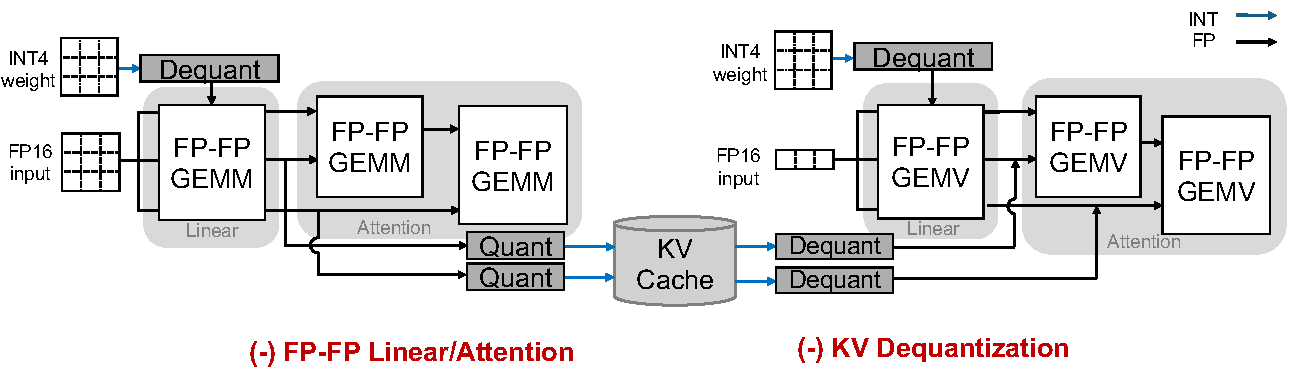
\includegraphics[width=0.95\linewidth]{figures/fig1_a.pdf}
        \caption{A conventional GPU dequantizes INT weight and KV operands before FP GEMM.}
        \label{fig:conventional-gpu}
    \end{subfigure}
    \vspace{0.5em}
    \begin{subfigure}[t]{\linewidth}
        \centering
        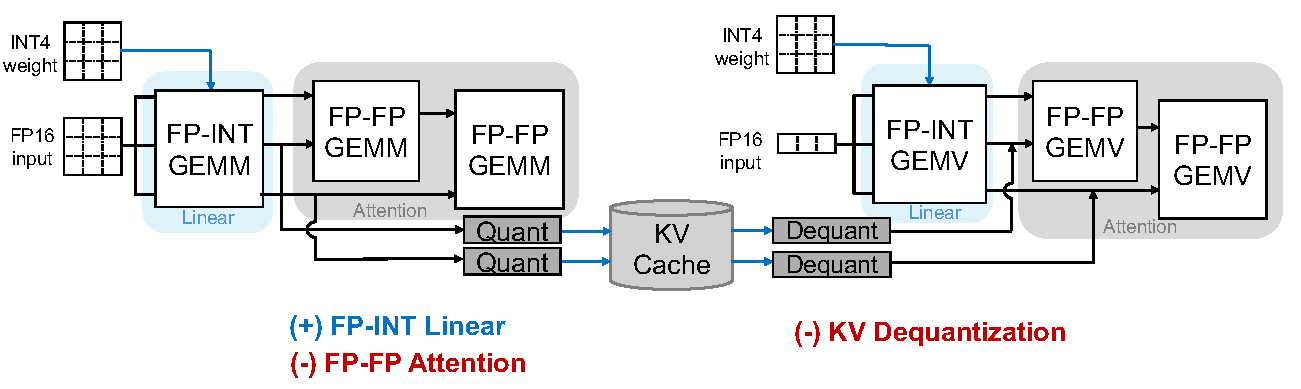
\includegraphics[width=0.95\linewidth]{figures/fig1_b.pdf}
        \caption{Prior \fpint{} accelerators support linear layers but leave attention on the FP path.}
        \label{fig:prior-fpint}
    \end{subfigure}
    \vspace{0.5em}
    \begin{subfigure}[t]{\linewidth}
        \centering
        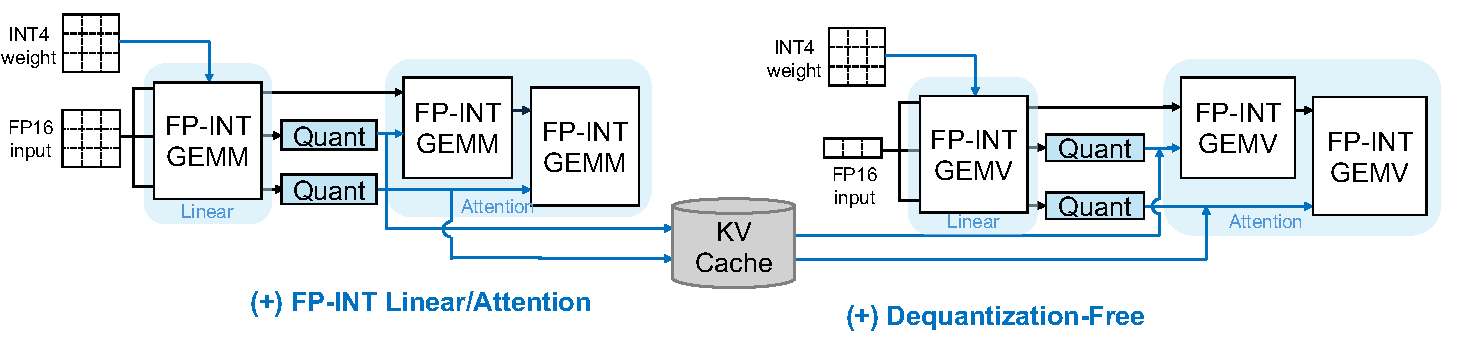
\includegraphics[width=0.99\linewidth]{figures/fig1_c.pdf}
        \caption{The proposed design executes both linear and attention GEMMs using native \fpint{} datapaths.}
        \label{fig:target-fpint}
    \end{subfigure}
    \caption{Comparison of \wkv{}-quantized inference datapaths.}
    \label{fig:fpint_inference}
\end{figure}

\subsection{Why Memory Savings Alone Are Insufficient}

Prefill is generally compute-bound~\cite{agrawal2024taming,patel2024splitwise}. Decode is often memory-bound, but batching, GQA, MQA, MLA, and quantization increase arithmetic intensity~\cite{orca,pagedattention}. The roofline analysis in Fig.~\ref{fig:bottleneck-analysis} motivates processing quantized operands directly, rather than only reducing traffic before FP execution~\cite{llm-analysis-chengli}.

\begin{figure}[t]
    \centering
    \begin{subfigure}[t]{\linewidth}
        \centering
        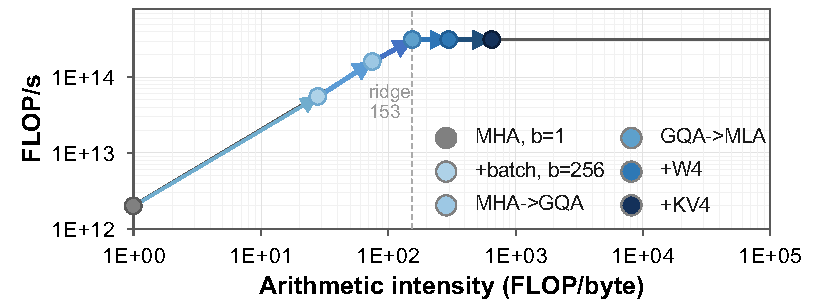
\includegraphics[width=0.92\linewidth]{figures/roofline_decode.pdf}
        \caption{Decode with a sequence length of 1024.}
        \label{fig:roofline_decode}
    \end{subfigure}
    \vspace{0.5em}
    \begin{subfigure}[t]{\linewidth}
        \centering
        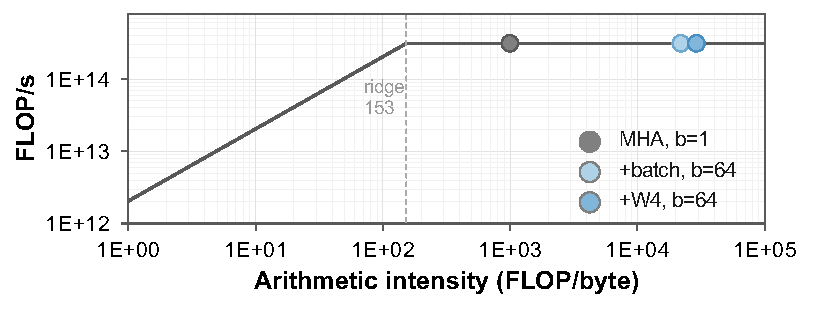
\includegraphics[width=0.92\linewidth]{figures/roofline_prefill.pdf}
        \caption{Prefill with a sequence length of 1024.}
        \label{fig:roofline_prefill}
    \end{subfigure}
    \caption{A100 FP16 roofline with a peak throughput of 312~TFLOP/s and a ridge point of 153~FLOP/byte\cite{a100}. Decode configurations progressively apply batch scaling, GQA, MLA, weight quantization, and KV-cache quantization, while prefill configurations apply batch scaling and weight quantization.}
    \label{fig:bottleneck-analysis}
\end{figure}

\subsection{Limitations of Software-based FP-INT Execution}

%Software \fpint{} GEMM kernels keep weights quantized in memory and fuse dequantization into the GEMM. 
%Existing GPU Tensor Cores, however, do not natively support GEMMs between FP activations and INT operands. 
%Each INT value must therefore be converted to FP before multiplication, and the dot product still executes on an FP$\times$FP Tensor Core. 
%Fusion can hide much of the conversion latency, so dequantization latency itself is not the fundamental limitation. 
%The fundamental limitation is that every MAC still incurs the cost of the FP$\times$FP datapath. 
%Software optimization therefore captures the memory benefit of quantization but cannot exploit the substantially higher compute density and energy efficiency of a dedicated \fpint{} unit~\cite{figna}.

Fused software FP-INT kernels retain quantized storage but convert operands to FP for every Tensor Core MAC. Fusion hides conversion latency, not its energy or the cost of FP arithmetic. Decode additionally dequantizes the accumulated KV cache for each generated token.

\begin{comment}
Although fusion can hide dequantization latency, our measurements show that
repeatedly converting the growing KV cache remains a first-order energy cost
during decode, accounting for an average of 77.4\% of decode energy when
linear layers use native \fpint{} execution but attention remains on the FP
path (Figure~\ref{fig:e2e-energy-dequant-breakdown}).
\end{comment}

\subsection{System-Level Limitations of Existing FP-INT Accelerators}
\label{sec:sys_gap}

FIGNA~\cite{figna} aligns FP mantissas to a shared exponent for integer MACs; FIGLUT~\cite{figlut} and LUT Tensor Core~\cite{lut_tensor_core} replace low-bit dot products with table lookups. These improve array-level efficiency but leave two system limitations.

\textbf{Limitation 1: Incomplete quantized-attention support.}
KV-cache schemes associate metadata with tokens or channels; group size separately determines how many elements share it (Table~\ref{tab:kv_quant_direction}). Both prefill and decode execute $QK^T$ and $PV$: prefill attention grows as $O(N^2)$ with sequence length, while decode repeatedly accesses the growing cache. FP fallback therefore limits both stages, especially long-sequence prefill (Fig.~\ref{fig:long_seq_atten_overhead}). Most prior \fpint{} designs accelerate only linear layers; AxCore~\cite{axcore} supports attention but lacks native channel-wise K and token-wise V quantization.

%AxCore considers quantized attention but does not natively support token-wise KV quantization~\cite{axcore}.

\begin{figure}[t]
    \centering
    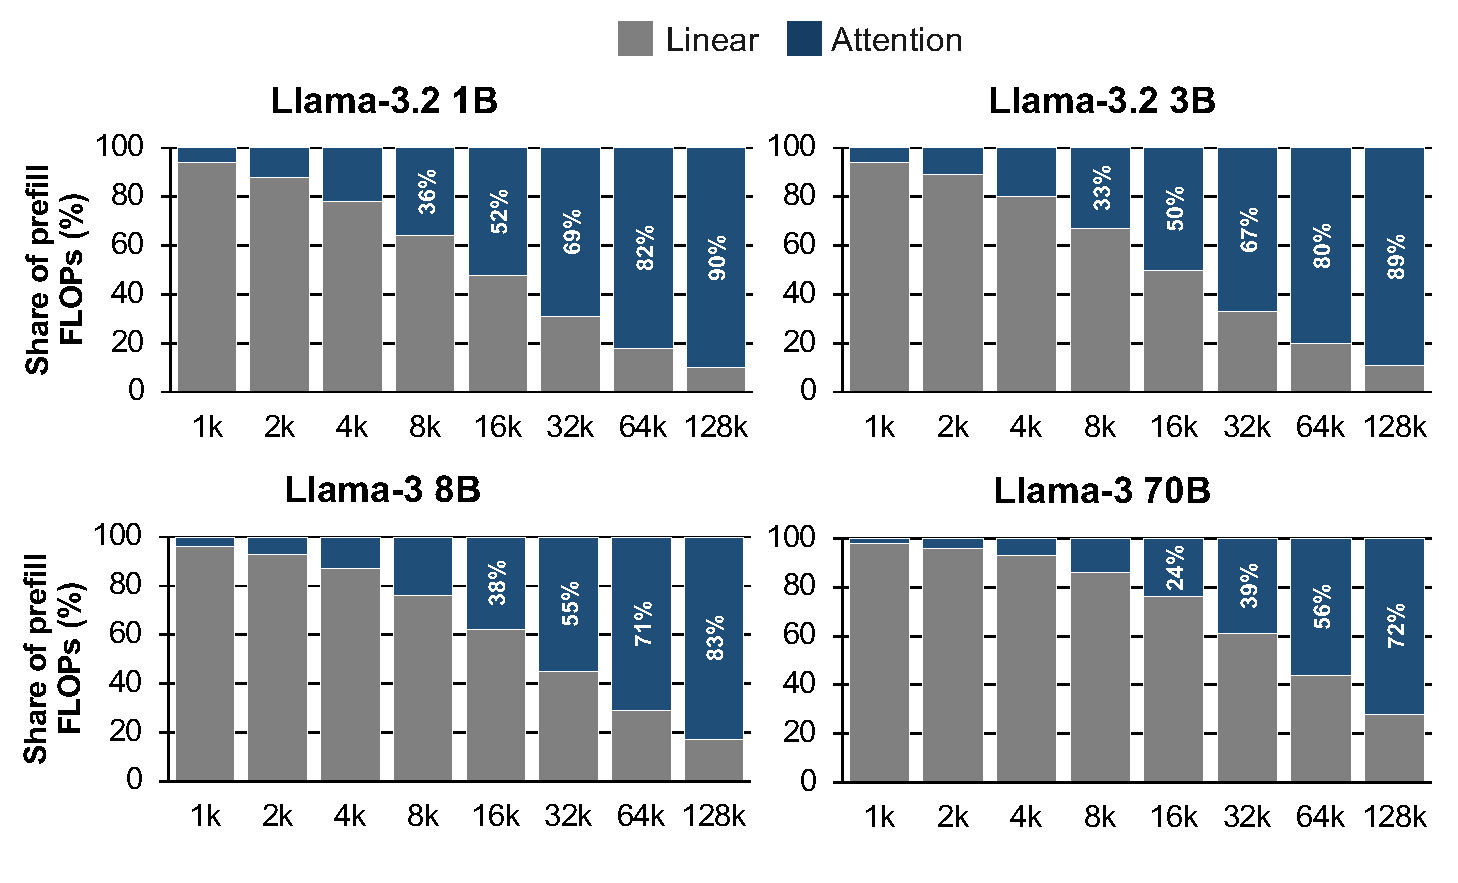
\includegraphics[width=0.92\linewidth]{figures/long_seq_attn_breakdown.pdf}
    \caption{Accelerating attention during prefill becomes critical in the long-sequence regime.}
    \label{fig:long_seq_atten_overhead}
\end{figure}

\begin{table}[t]
\centering
\caption{Quantization directions used by KV-cache quantization schemes.}
\label{tab:kv_quant_direction}
% \small
\setlength{\tabcolsep}{3pt}
\begin{tabularx}{\columnwidth}{@{}>{\raggedright\arraybackslash}Xcc@{}}
\toprule
Scheme & K Direction & V Direction \\
\midrule
KIVI~\cite{liu2024kivi} / KVQuant~\cite{hooper2024kvquant} / ZipCache~\cite{he2024zipcache} & channel-wise & token-wise \\
WKVQuant~\cite{yue2024wkvquant}  / QuaRot~\cite{ashkboos2024quarot} / SpinQuant~\cite{liu2024spinquant} & token-wise & token-wise \\
\bottomrule
\end{tabularx}
\end{table}

We define hardware quantization direction in the INT operand layout seen by the MXU: \qcol{} associates metadata with columns and \qrow{} with rows. The mapping from token/channel quantization depends on the operation and load orientation. Channel-wise K consumed transposed in $QK^T$ and token-wise V in $PV$ require \qrow{}. Their scales and zero points vary across reduction terms, so a conventional \qcol{} datapath cannot apply one correction after accumulation; per-term dequantization and FP reduction erode its efficiency (Fig.~\ref{fig:quant_row_dir_overhead}).

\begin{figure}[t]
    \centering
    \begin{subfigure}[t]{\linewidth}
        \centering
        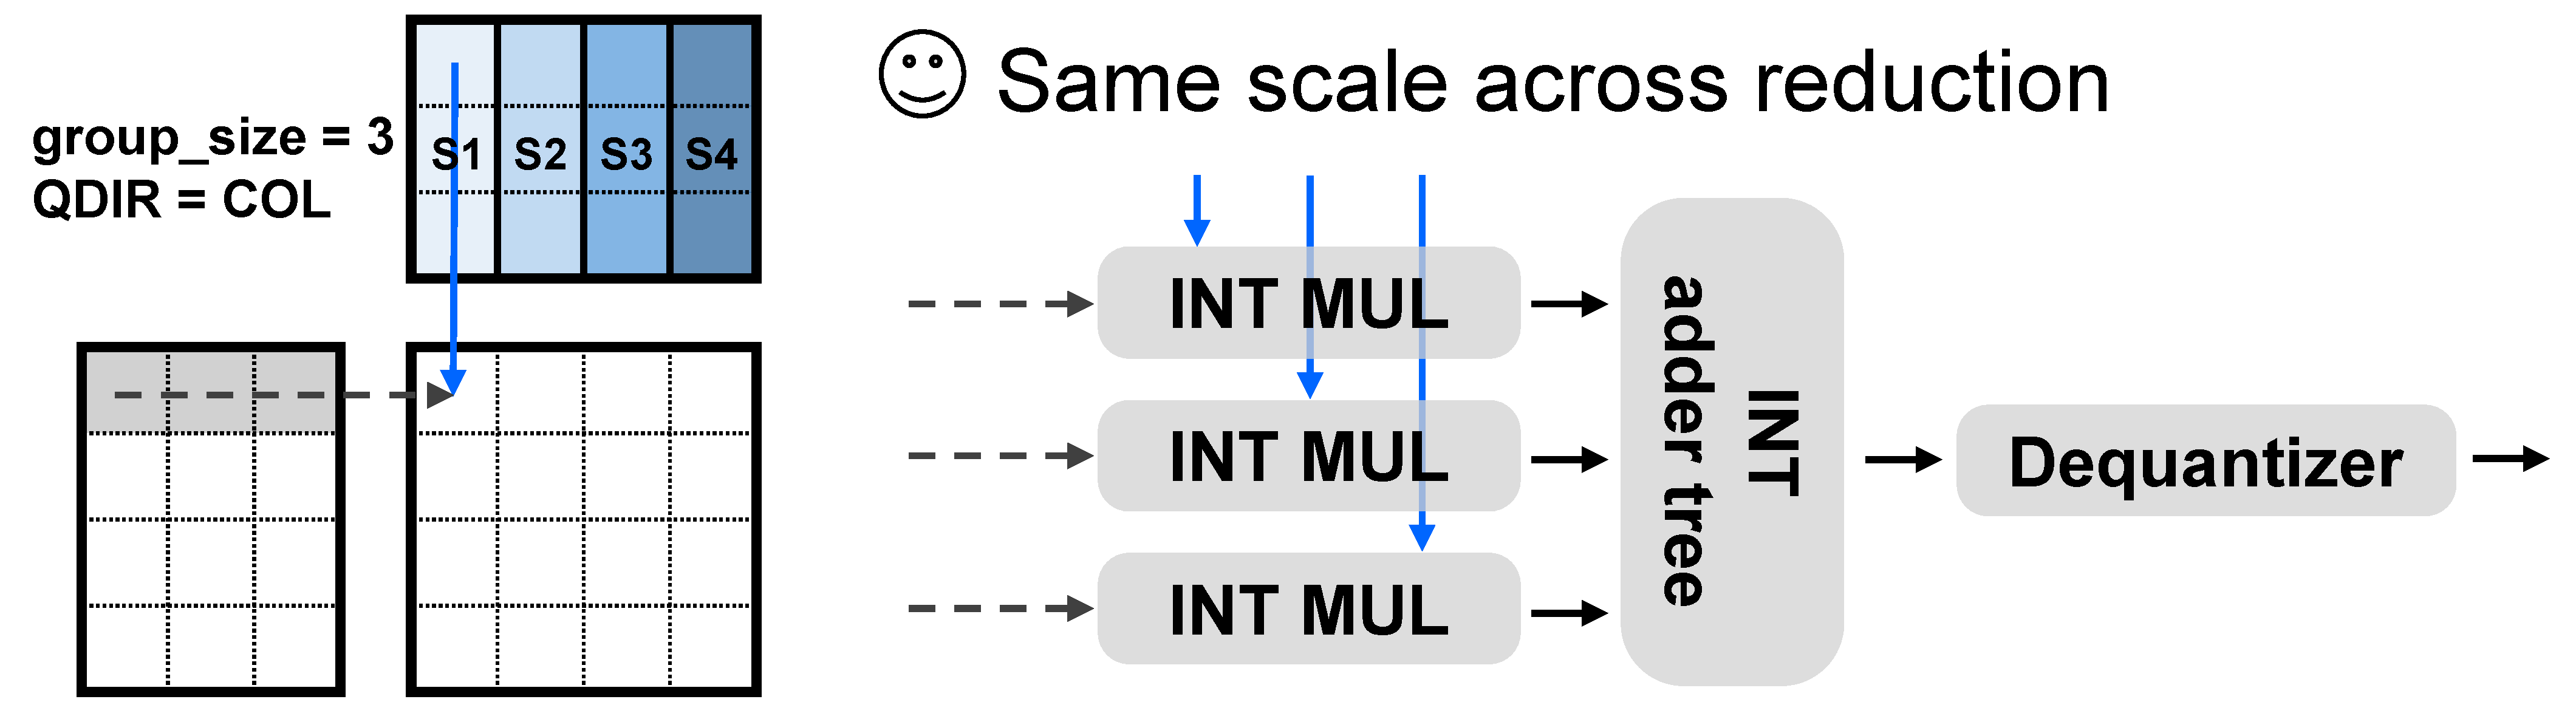
\includegraphics[width=0.87\linewidth]{figures/fig4_a.pdf}
        \caption{\qcol{} execution on a conventional FIGNA-style datapath.}
        \label{fig:conv_acc}
    \end{subfigure}
    \vspace{0.5em}
    \begin{subfigure}[t]{\linewidth}
        \centering
        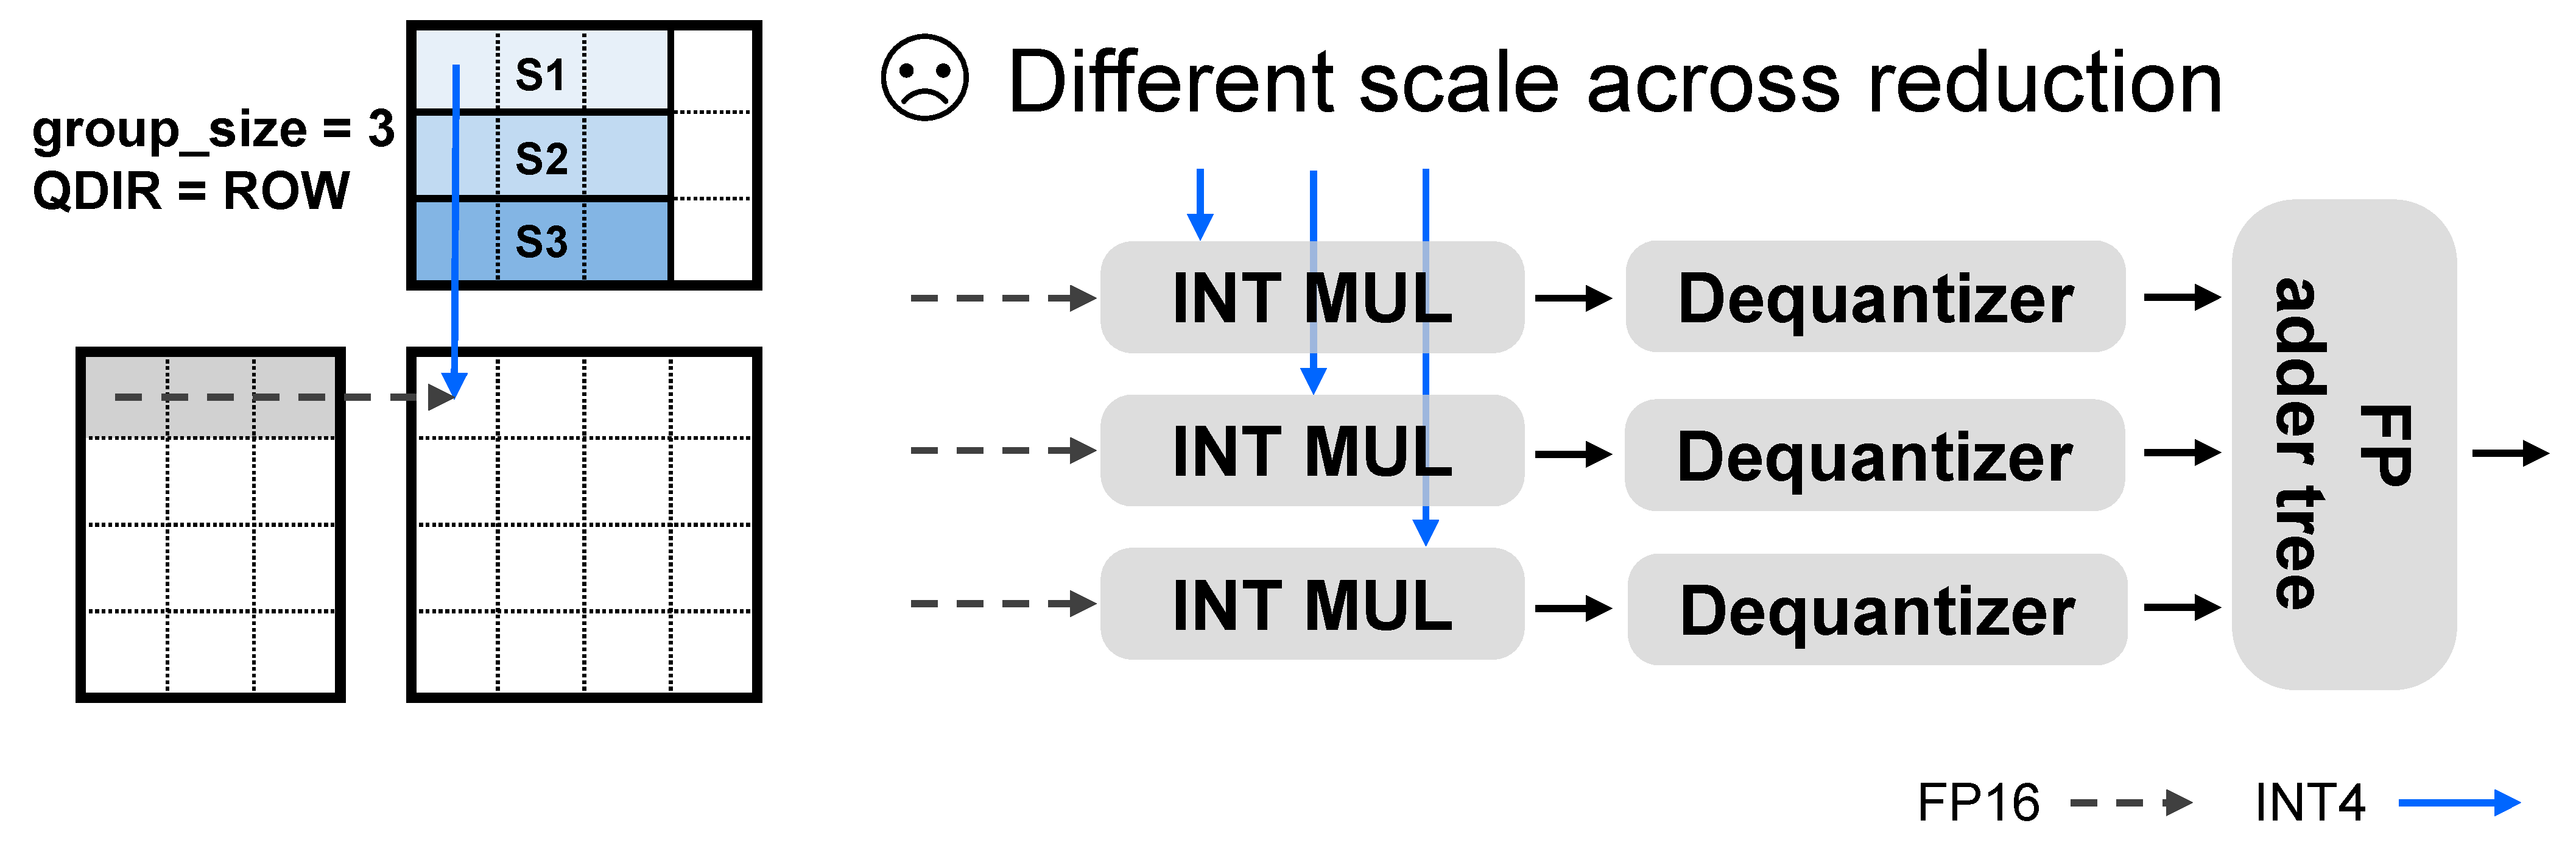
\includegraphics[width=0.87\linewidth]{figures/fig4_b.pdf}
        \caption{\qrow{} execution on a datapath designed only for \qcol{}.}
        \label{fig:row_quant}
    \end{subfigure}
    %\caption{\qrow{} introduces per-term dequantization and FP-reduction overhead on an accelerator designed only for \qcol{}.}
    \caption{\qrow{} introduces per-term dequantization and FP-reduction overhead.}
    \label{fig:quant_row_dir_overhead}
\end{figure}

\textbf{Limitation 2: Operand delivery erodes array-level gains.}
A denser MXU needs matching operand, partial-sum, and command bandwidth. Conventional GPU memory hierarchies provide flexible access through crossbars~\cite{jin2024uncovering,tine2021vortex}. Scaling their ports and banks with an \fpint{} array increases interconnect and peripheral area, diminishing its TOPS/mm$^2$ advantage (Fig.~\ref{fig:xbar_overhead}).


\begin{figure}[t]
    \centering
    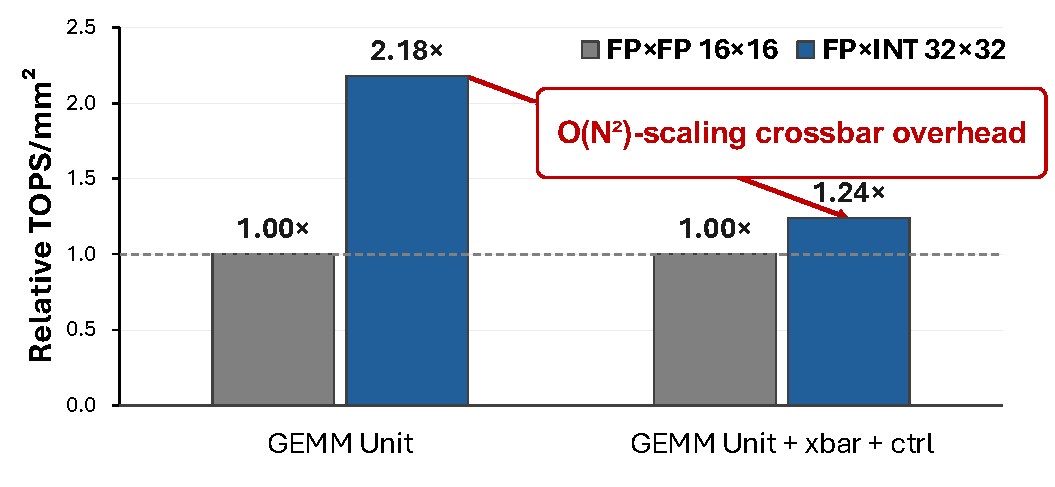
\includegraphics[width=0.82\linewidth]{figures/fig5.pdf}
    \caption{Relative TOPS/mm$^2$ of FP$\times$FP and \fpint{} GEMM units as crossbar and memory-system areas are included. Areas are obtained from Synopsys Design Compiler synthesis in a 28 nm CMOS technology.
    To move the design toward the ridge point of the GEMV roofline,
    the local-memory bank count increases from 16 to 64, the data-cache bank count from 2 to 8, and the number of HBM access ports from 2 to 8.}
    \label{fig:xbar_overhead}
\end{figure}


%Jae-Joon
\section{Overview of The Proposed \ours{} System}
\label{sec:overview}

\begin{figure*}[t]
    \centering
    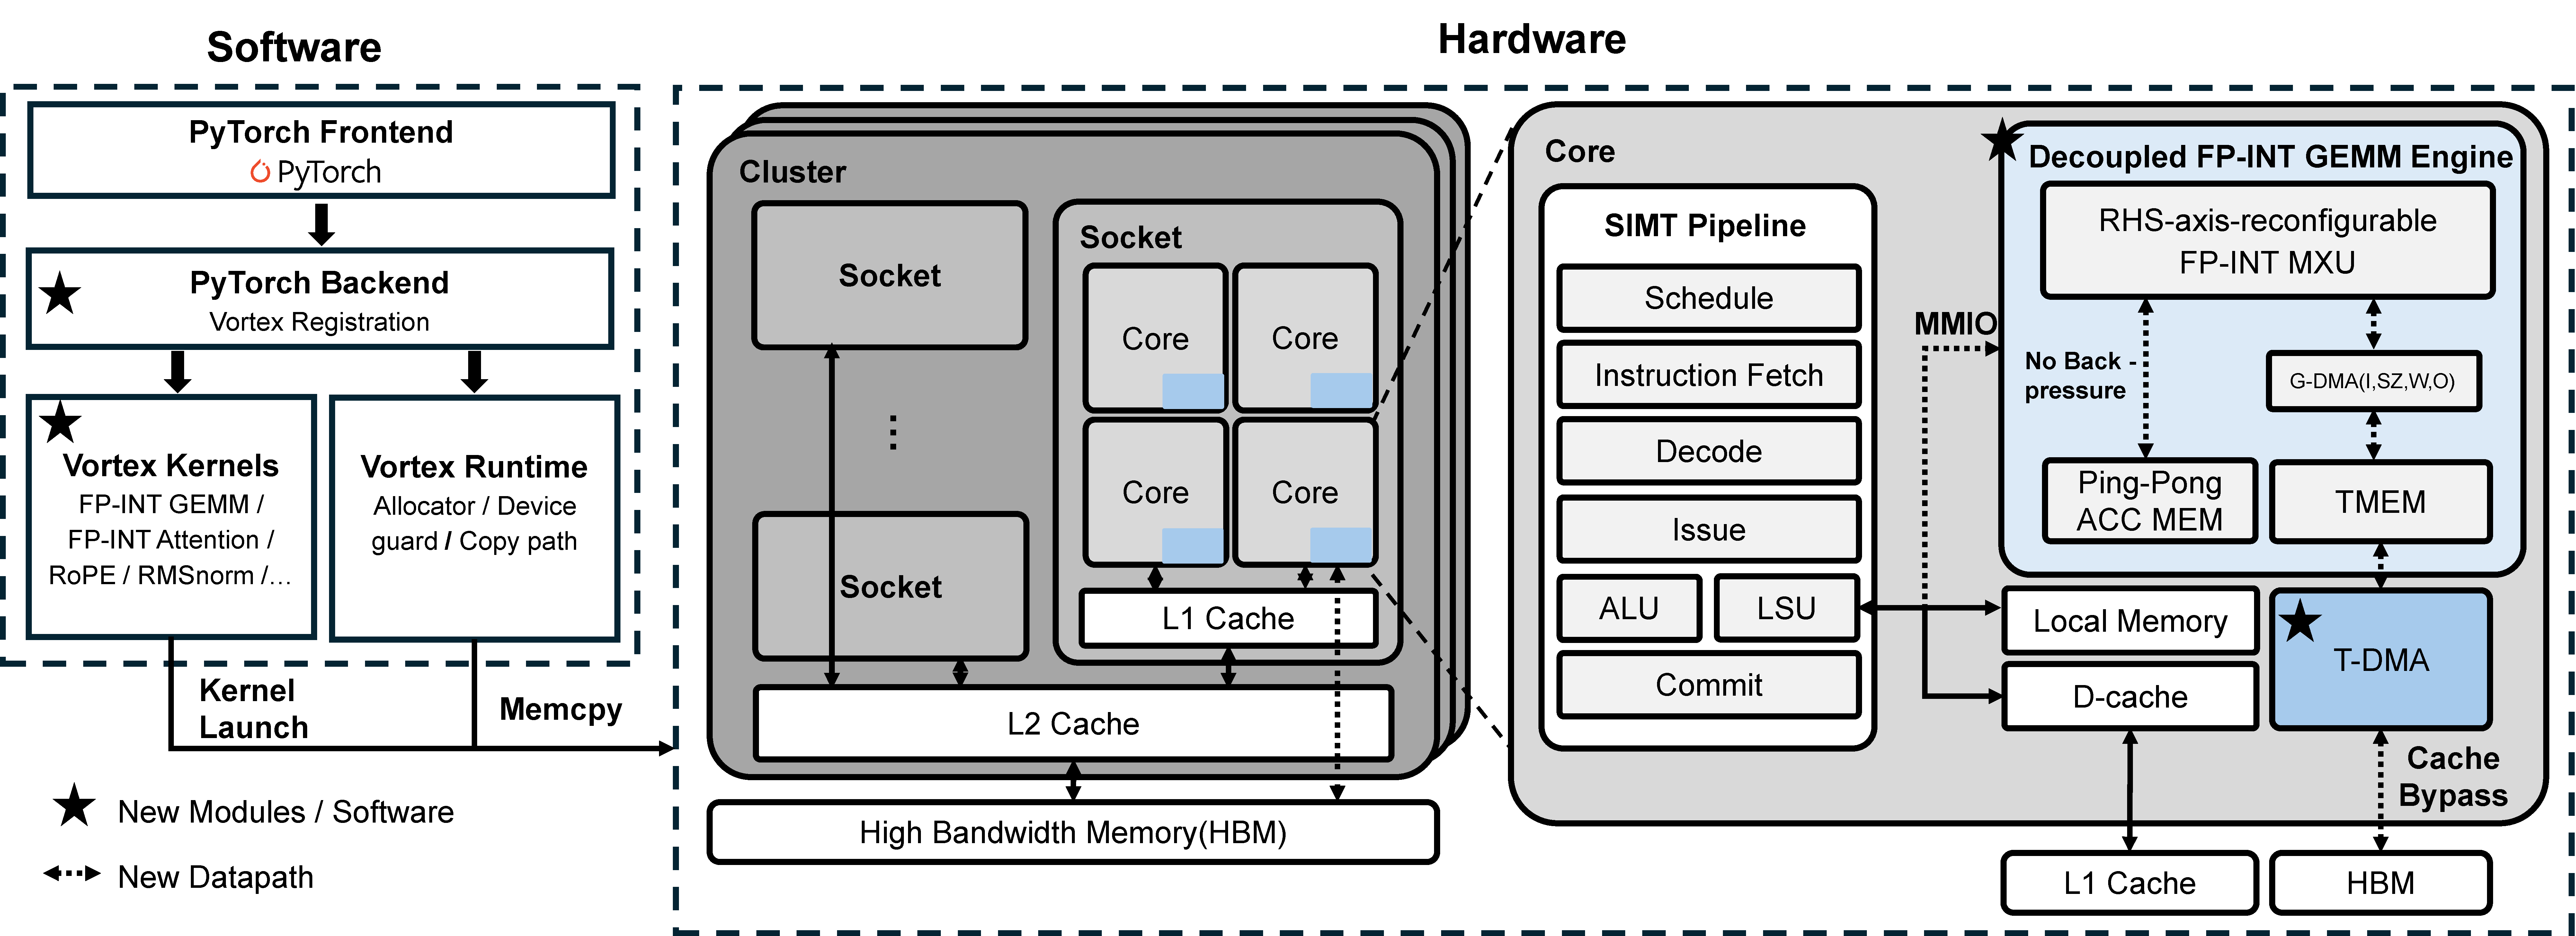
\includegraphics[width=0.90\linewidth]{figures/top_diagram.pdf}
    \caption{Overview of the \ours{} hardware/software system and its end-to-end execution flow.}
    \label{fig:overview}
\end{figure*}


\subsection{Overall Architecture}
% ---------------------------------------------------------------------
% \ours{} is an end-to-end hardware/software system for LLM inference with quantized weights and KV cache. It builds on 
% Vortex~\cite{tine2021vortex}, an open-source GPGPU, and integrates a native \fpint{} GEMM engine with a dedicated tensor-memory subsystem and the runtime and kernel support required to use it. 
% Figure~\ref{fig:overview} shows the high-level organization of \ours{}.
% LLM inference contains control flow and vector operations, including normalization, activation functions, softmax, elementwise operations, quantization, and layout manipulation, in addition to GEMMs. Although these vector operations account for a relatively small fraction of the total arithmetic work, offloading them to a host CPU would incur frequent synchronization and data-transfer overheads. The orignal Vortex SIMT pipeline therefore remains responsible for control flow, vector kernels, kernel launch, and synchronization, while a decoupled \fpint{} GEMM engine executes the linear and attention GEMMs through memory-mapped IO (MMIO)-issued descriptors.
% ---------------------------------------------------------------------
% +++++++++++++++++++++++++++++++++++++++++++++++++++++++++++++++++++++
Built on Vortex~\cite{tine2021vortex}, \ours{} couples a native \fpint{} GEMM engine to dedicated tensor memory (Fig.~\ref{fig:overview}). The SIMT pipeline retains control flow, kernel launch, synchronization, and vector operations including normalization, activation, softmax, quantization, and layout manipulation. It invokes the decoupled GEMM engine through memory-mapped IO (MMIO) descriptors.
% +++++++++++++++++++++++++++++++++++++++++++++++++++++++++++++++++++++

%To make the end-to-end FP-INT LLM inference system more effective, we introduce several design features as follows.

\subsection{Quantization-Direction-Aware Reconfigurable Dataflow}
% The \fpint{} GEMMs in a \wkv{}-quantized model differ in how quantization metadata is organized for the INT operand and whether that operand is presented to the MXU in standard or transposed form. 
% \ours{} captures these differences using two independent, per-GEMM configuration attributes: (1) quantization direction (\qcol{} or \qrow{}), (2) Loading choice for quantized operand (Standard or Transposed), as summarized in Table~\ref{tab:gemm-config}.

\begin{table}[t]
  \centering
  \caption{FINISH configurations for FP-INT GEMMs.}
  \label{tab:gemm-config}
  %\scriptsize
  \renewcommand{\arraystretch}{0.95}
  \begin{tabular*}{\columnwidth}
    {@{\extracolsep{\fill}}lccc@{}}
  \toprule
  GEMM & INT operand direction & QDir & Load \\
  \midrule
  Linear & channel        & Q-COL & Standard \\
  $QK^T$ & token/channel  & Q-COL/Q-ROW & Transposed \\
  $PV$   & token/channel  & Q-ROW/Q-COL & Standard \\
  \bottomrule
  \end{tabular*}
\end{table}

\begin{comment}
\ours{} captures these differences using two independent, per-GEMM configuration attributes: (1) quantization direction (\qcol{} or \qrow{}), (2) Loading choice for quantized operand (Standard or Transposed)(Table~\ref{tab:gemm-config}).
\begin{table}[t]
  \centering
  \caption{FINISH configurations for FP-INT GEMMs.}
  \label{tab:gemm-config}
  \scriptsize
  \setlength{\tabcolsep}{2.5pt}
  \begin{tabular}{@{}lccc@{}}
  \toprule
  GEMM & INT operand & QDir & Load \\
  \midrule
  Linear & W group-wise    & Q-COL & Std. \\
  $QK^T$ & K token-wise   & Q-COL & Trans. \\
  $QK^T$ & K channel-wise & Q-ROW & Trans. \\
  $PV$   & V token-wise   & Q-ROW & Std. \\
  $PV$   & V channel-wise & Q-COL & Std. \\
  \bottomrule
  \end{tabular}
\end{table}
\end{comment}
%The quantization direction selects either \qcol{} or \qrow{} metadata handling, while the load orientation selects standard or transposed loading of the INT operand. Linear projections, FFN layers, and $PV$ use the standard orientation, whereas $QK^T$ consumes K in transposed orientation. As summarized in Table~\ref{tab:kv_quant_direction}, token-wise and channel-wise quantization of the original K and V tensors map differently to \qcol{} and \qrow{} depending on the operation and load orientation. 
% By configuring these two attributes independently, the same physical \fpint{} GEMM engine in FINISH can support the required execution modes across linear and attention layers with minimal hardware overhead. Section~\ref{sec:fpint-gemm-engine} details the corresponding datapaths and execution mechanisms.
\ours{} exposes two independent per-GEMM attributes, the quantization direction (Q-COL or Q-ROW) and the operand load orientation (standard or transposed). Table~\ref{tab:gemm-config} lists their settings for the linear, $QK^T$, and $PV$ GEMMs. Configuring the two attributes independently lets one physical FP-INT array cover all three cases. Section~\ref{sec:fpint-gemm-engine} details the corresponding datapaths.

% ---------------------------------------------------------------------
% \subsection{Tensor Memory System and Data Path for Improved GEMM Engine Utilization}
% Naively scaling a conventional crossbar-based memory system with a denser \fpint{} MXU can diminish its array-level TOPS/mm$^2$ advantage.
% To efficiently feed the larger number of FP-INT MACs over conventional FP-FP MACs, FINISH employs dedicated memory (TMEM) and datapath for Tensor data, which separates regular tensor traffic from general-purpose SIMT load/store traffic.
% The dedicated tensor path allow \ours{} to increase \fpint{} compute density without proportionally scaling the register-file, cache, and local-memory interconnects. Detailed discussions are given in Section~\ref{sec:memory-system}.
% %To efficiently feed the larger number of FP-INT MACs over conventional FP-FP MACs, FINISH employs dedicated memory for Tensor data (TMEM). Tensor operands are transferred among HBM pseudo-channels, TMEM, and the GEMM engine through a cache-bypassing, high-bandwidth tensor path. This path separates regular tensor traffic from general-purpose SIMT load/store traffic. Dedicated accumulator memory keeps wide partial sums off the input and weight paths, preventing accumulation traffic from interfering with operand delivery. Together, the decoupled GEMM engine and the dedicated tensor path allow \ours{} to increase \fpint{} compute density without proportionally scaling the register-file, cache, and local-memory interconnects. Detailed discussions are given in Section~\ref{sec:memory-system}.

% \subsection{Hardware Constraint-Aware Data Mapping and Allocation}
% The dedicated TMEM and tensor datapath with simplified connectivity trades general address flexibility for lower hardware overhead. 
% Because GEMM tensors exhibit regular tiled access patterns, \ours{} satisfies these constraints through alignment-aware HBM allocation and compatible tensor layouts. 
% %This design scales the available tensor-memory bandwidth to $8\times$ that of the baseline with only an approximately 4\% increase in total area. 
% This design scales the available HBM-to-tensor-memory bandwidth to $8\times$ that of the baseline with only an  5.22\% increase in total area.
% Detailed discussions are given in Section~\ref{sec:runtime-section}.
% ---------------------------------------------------------------------
% +++++++++++++++++++++++++++++++++++++++++++++++++++++++++++++++++++++
\subsection{Dedicated Tensor Path with Constraint-Aware Software Support}
Dedicated tensor memory (TMEM) separates regular GEMM traffic from general-purpose SIMT accesses~\cite{dissecting_hopper,virgo}. Restricted connectivity lowers hardware cost (Section~\ref{sec:memory-system}); aligned allocation and tiled layouts satisfy its address constraints (Section~\ref{sec:runtime-section}). The tensor path provides $8\times$ the baseline HBM-to-TMEM bandwidth, while DMA and interconnect logic occupy 5.5\% of total area.
% +++++++++++++++++++++++++++++++++++++++++++++++++++++++++++++++++++++

\subsection{Hardware-Generated GEMM Command Stream}
A large \fpint{} MXU needs command bandwidth as well as operand bandwidth. 
On Vortex, generating tile-level commands on SIMT lanes became a GEMM-launch bottleneck. 
FINISH instead has the kernel write a compact MMIO descriptor containing the matrix and tile dimensions, operand addresses, quantization direction (QDir), and load direction, which a hardware FSM expands into DMA, MXU, accumulation, and completion micro-ops.
% In our initial design, a kernel built tile-level commands through bit manipulation and enqueued them with store instructions, but on Vortex this scalar command stream became the launch bottleneck. 
% FINISH instead has the kernel write the matrix dimensions, tile dimensions, tensor, accumulator, scale, and zero-point base addresses, quantization direction (qdir), and load direction to MMIO registers, and then initiate execution by writing 1 to the start bit in the MMIO registers.
% A micro-op FSM inside the GEMM engine expands the descriptor into DMA, load direction of the quantized input, MXU step, accumulator update, and completion signaling. 
% The SIMT pipeline therefore handles compact descriptor setup and synchronization, while hardware generates the repetitive GEMM command stream.

%Jae-Joon
\begin{comment}
\section{\ours{} Design Overview}

\begin{figure*}[t]
    \centering
    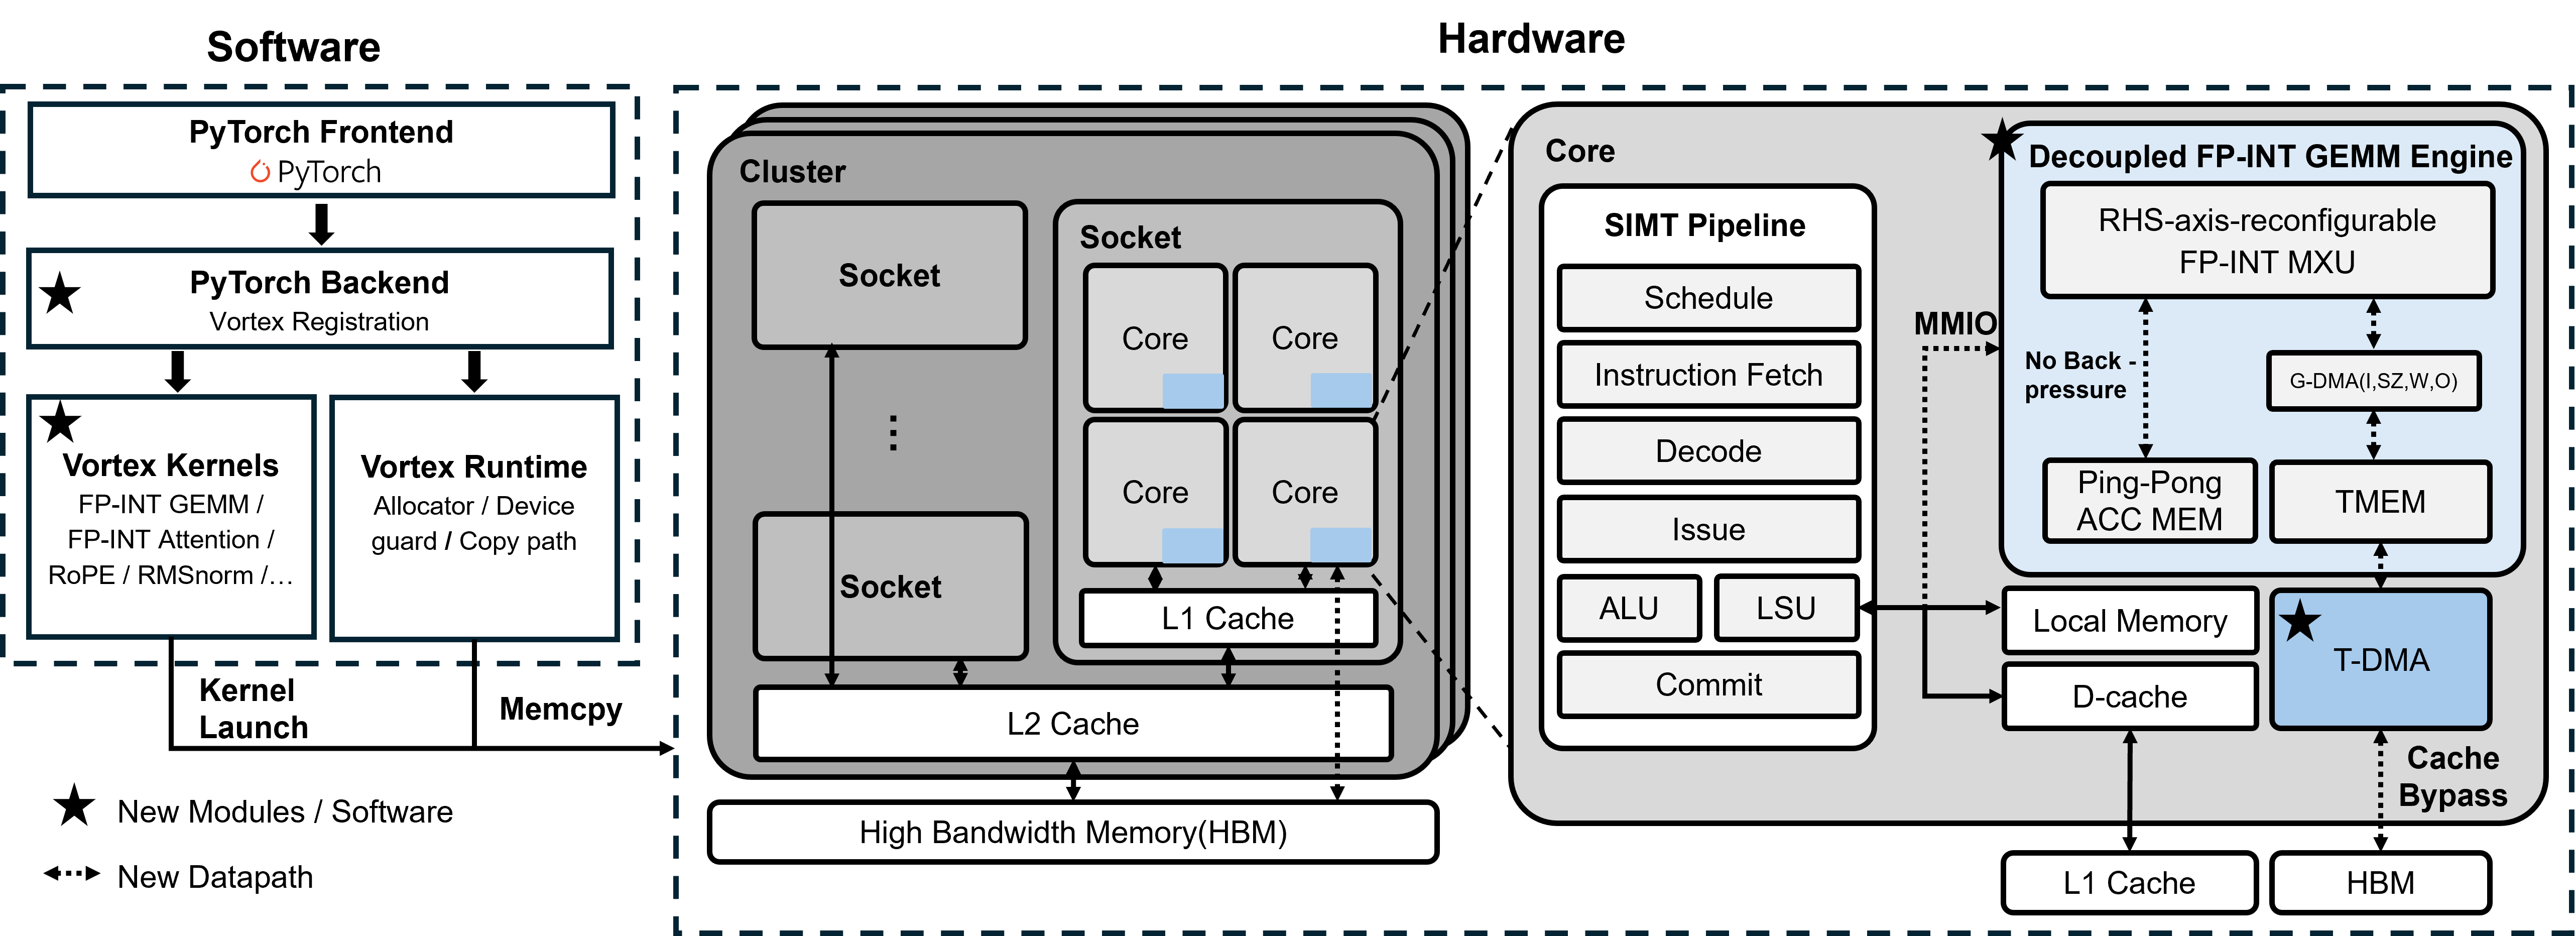
\includegraphics[width=0.95\linewidth]{figures/top_diagram.png}
    \caption{Overview of the proposed hardware/software system.}
    \label{fig:overview}
\end{figure*}

\ours{} is built on Vortex~\cite{tine2021vortex}, an open source GPGPU, and accelerates WKV quantized models by integrating an \fpint{} GEMM engine with an efficient memory subsystem and the runtime and kernel support required to use it.
Figure~\ref{fig:overview} shows the high-level organization of \ours{}.
The original Vortex SIMT pipeline remains responsible for control flow, vector operations, kernel launch, and synchronization, while a decoupled \fpint{} GEMM engine executes the linear and attention GEMMs through MMIO-issued descriptors.
%Tensor operands move between HBM pseudo channels, tensor memory, and the GEMM engine through a cache bypassed direct tensor path. 
Tensor operands are transferred among HBM pseudo-channels, tensor memory, and the GEMM engine through a cache-bypassing, high-bandwidth tensor data path equipped with DMA units that support aligned access across multiple channels.
The runtime and kernels manage layout, alignment, and synchronization so that this restricted path can be used efficiently.
To make this system effective end-to-end, we make several design decisions.

\textbf{Retaining the Vortex SIMT pipeline.}
An LLM contains a variety of vector operations in addition to GEMM. Even though these vector operations carry a small fraction of the total work, falling back to a CPU for them would incur a large overhead. We therefore keep the SIMT pipeline to preserve programmability and generality.

% \paragraph{The \fpint{} GEMM engine must support every combination of quantization direction and load direction for the right hand side operand.}
\textbf{Reconfigurable quantization and load directions for the right hand side.}
The \fpint{} GEMMs that appear repeatedly in a \wkv{} quantized model vary along two hardware axes for the RHS operand of the MXU. The RHS quantization direction is either \qcol{} or \qrow{}. The RHS load direction determines whether the operand is consumed in its standard or transposed orientation. In QK$^T$, the RHS must be consumed in transposed form, whereas in PV, the linear projections, and the FFN, the RHS is not transposed. Table~\ref{tab:kv_quant_direction} describes the token-wise and channel-wise quantization directions of the original K and V tensors. Their mapping to \qcol{} or \qrow{} depends on the operation and the RHS load direction. The \fpint{} GEMM engine must therefore support all four hardware execution patterns in a reconfigurable manner.

% \paragraph{We decouple the GEMM engine from SIMT and use dedicated tensor memory and accumulator memory.}
\textbf{Decoupled GEMM engine with a dedicated tensor path.}
Virgo previously demonstrated that a matrix unit can be physically disaggregated from the SIMT cores and placed at the GPU cluster level. This organization bypasses the capacity and bandwidth limitations of the SIMT register file and also supports separate accumulator memory~\cite{virgo}. We build on this established organization for a denser \fpint{} engine and focus on supplying the data bandwidth needed to keep it utilized. Virgo supplies matrix operands through cluster shared memory. For our \fpint{} engine, scaling the shared memory crossbar to the required bandwidth would be costly, and SIMT load and store traffic could interfere with tensor traffic. \ours{} therefore uses dedicated tensor memory and places accumulator memory inside the GEMM engine. The accumulator memory keeps wider partial sums off the input and weight path and enables a conflict free ping pong schedule on two single port SRAMs, so the GEMM pipeline can run without back pressure.

% \paragraph{The GEMM command stream is generated by a hardware micro-op FSM, not by a software queue.}
\textbf{Hardware-generated GEMM command stream.}
A large \fpint{} MXU needs command bandwidth as well as operand bandwidth. In our initial design, a kernel built tile-level commands through bit manipulation and enqueued them with store instructions, but on Vortex this scalar command stream became the launch bottleneck. 
%\ours{} instead has the kernel write the matrix shape, tile shapes, tensor/accumulator/scale/zero-point base addresses, quantization direction (\texttt{qdir}), and load direction into MMIO registers, then submit the request through a doorbell.
FINISH instead has the kernel write the matrix dimensions, tile dimensions, tensor, accumulator, scale, and zero-point base addresses, quantization direction (qdir), and load direction to MMIO registers, and then initiate execution by writing 1 to the start bit in the MMIO registers.
A micro-op FSM inside the GEMM engine expands the descriptor into DMA, RHS load, MXU step, accumulator update, and completion signaling. The SIMT pipeline therefore handles compact descriptor setup and synchronization, while hardware generates the repetitive GEMM command stream.

% \paragraph{Rather than scaling the memory subsystem with a complex crossbar, we scale it at low cost with a simple interconnect fabric and handle the resulting constraints in the software stack.}
\textbf{Low-Cost, Restricted Interconnect with Software-Handled Constraints.}
Naively scaling full-crossbar memory components can eliminate the TOPS/mm$^2$ gain of the \fpint{} array. At the HBM--TMEM boundary, \ours{} replaces a full crossbar with a fixed 1:1 or interleaved fabric. At the TMEM--MXU boundary, four fixed 64\,B GEMM ports select among the TMEM banks through restricted wide-word mux/demux paths. Tensor traffic is carried on a cache-bypassed DMA path. When a vector stage is fused before GEMM, it issues a fence after producing the GEMM inputs. When a vector stage follows GEMM, it polls a read-only MMIO register that reports completed result tiles. The tradeoff is a set of boundary-specific mapping and alignment constraints that the software stack must satisfy.
%Because GEMM traffic is regular, constraint-aware HBM allocation and tensor layout can satisfy these constraints while scaling memory bandwidth by $8\times$ with only about a 4\% increase in total area.
Because GEMM traffic exhibits regular access patterns, constraint-aware HBM allocation and tensor layouts can satisfy these requirements while scaling memory bandwidth to $8\times$ the baseline, with only an approximately 4\% increase in total area.
\end{comment}

\section[Quantization-Direction-Reconfigurable FP-INT GEMM Engine]{Quantization-Direction-Reconfigurable \texorpdfstring{\fpint{}}{FP-INT} GEMM Engine}
\label{sec:fpint-gemm-engine}

As discussed in Section~\ref{sec:sys_gap}, native \fpint{} attention requires supporting both \qcol{} and \qrow{} quantization directions. In \qrow{}, the quantization metadata varies along the GEMM reduction dimension, preventing a conventional \qcol{} datapath from applying scale and zero-point correction only after accumulation.

% ---------------------------------------------------------------------
% To support both directions efficiently, we propose an \fpint{} MXU that independently configures the quantization direction and the load orientation of the quantized operand. We denote the FP input operand as matrix $A$ and the quantized weight or KV operand as matrix $B^{\mathrm{int}}$. Let $G_K$ and $G_N$ denote the quantization group sizes along the reduction and output dimensions, respectively, with $g(k)=\lfloor k/G_K \rfloor$ and $h(n)=\lfloor n/G_N \rfloor$. We use $\mathcal{K}_g$ to denote the set of reduction indices in group $g$. 
% Depending on the quantization direction, one of the \qcol{} or \qrow{} scaling and zero-point-correction path is selected. In addition, $B^{\mathrm{int}}$ is loaded in the standard of transposed orientation accordingly.
% %The \texttt{qdir} field selects the \qcol{} or \qrow{} scaling and zero-point-correction path, while a separate field selects whether $B^{\mathrm{int}}$ is loaded in its standard or transposed orientation.
% We design both \qcol{} and \qrow{} to share the prealigner and integer multiply-accumulate datapath to minimize the overhead to support both modes.
% %Both modes share the prealigner and integer multiply-accumulate datapath.
% For implementation, we follow the numerical-accuracy-preserving prealignment scheme of FIGNA~\cite{figna}, representing each FP16 input using a 31-bit signed aligned mantissa before integer multiplication and reduction. The subsequent integer accumulation and conversion back to FP also adopt FIGNA style. The proposed extensions determine where scale multiplication is performed, how zero-point correction is ordered, and how the quantized operand is loaded into the MXU.
% ---------------------------------------------------------------------
% +++++++++++++++++++++++++++++++++++++++++++++++++++++++++++++++++++++
We therefore propose an \fpint{} MXU that independently selects the quantization direction (\qcol{} or \qrow{}) and the load orientation (standard or transposed) of the quantized operand. We denote the FP input as $A$ and the quantized weight or KV operand as $B^{\mathrm{int}}$; $G_K$ and $G_N$ are the quantization group sizes along the reduction and output dimensions, with $g(k)=\lfloor k/G_K \rfloor$, $h(n)=\lfloor n/G_N \rfloor$, and $\mathcal{K}_g$ the reduction indices in group $g$. Both modes share the prealigner and integer multiply-accumulate datapath to minimize the cost of supporting both. We follow the numerical-accuracy-preserving prealignment of FIGNA~\cite{figna}, representing each FP16 input as a 31-bit signed aligned mantissa before integer multiplication and reduction, and adopt its integer accumulation and FP conversion. Our extensions determine where the scale is applied, how zero-point correction is ordered, and how $B^{\mathrm{int}}$ is loaded.
% ---------------------------------------------------------------------

\begin{figure}[t]
    \centering
    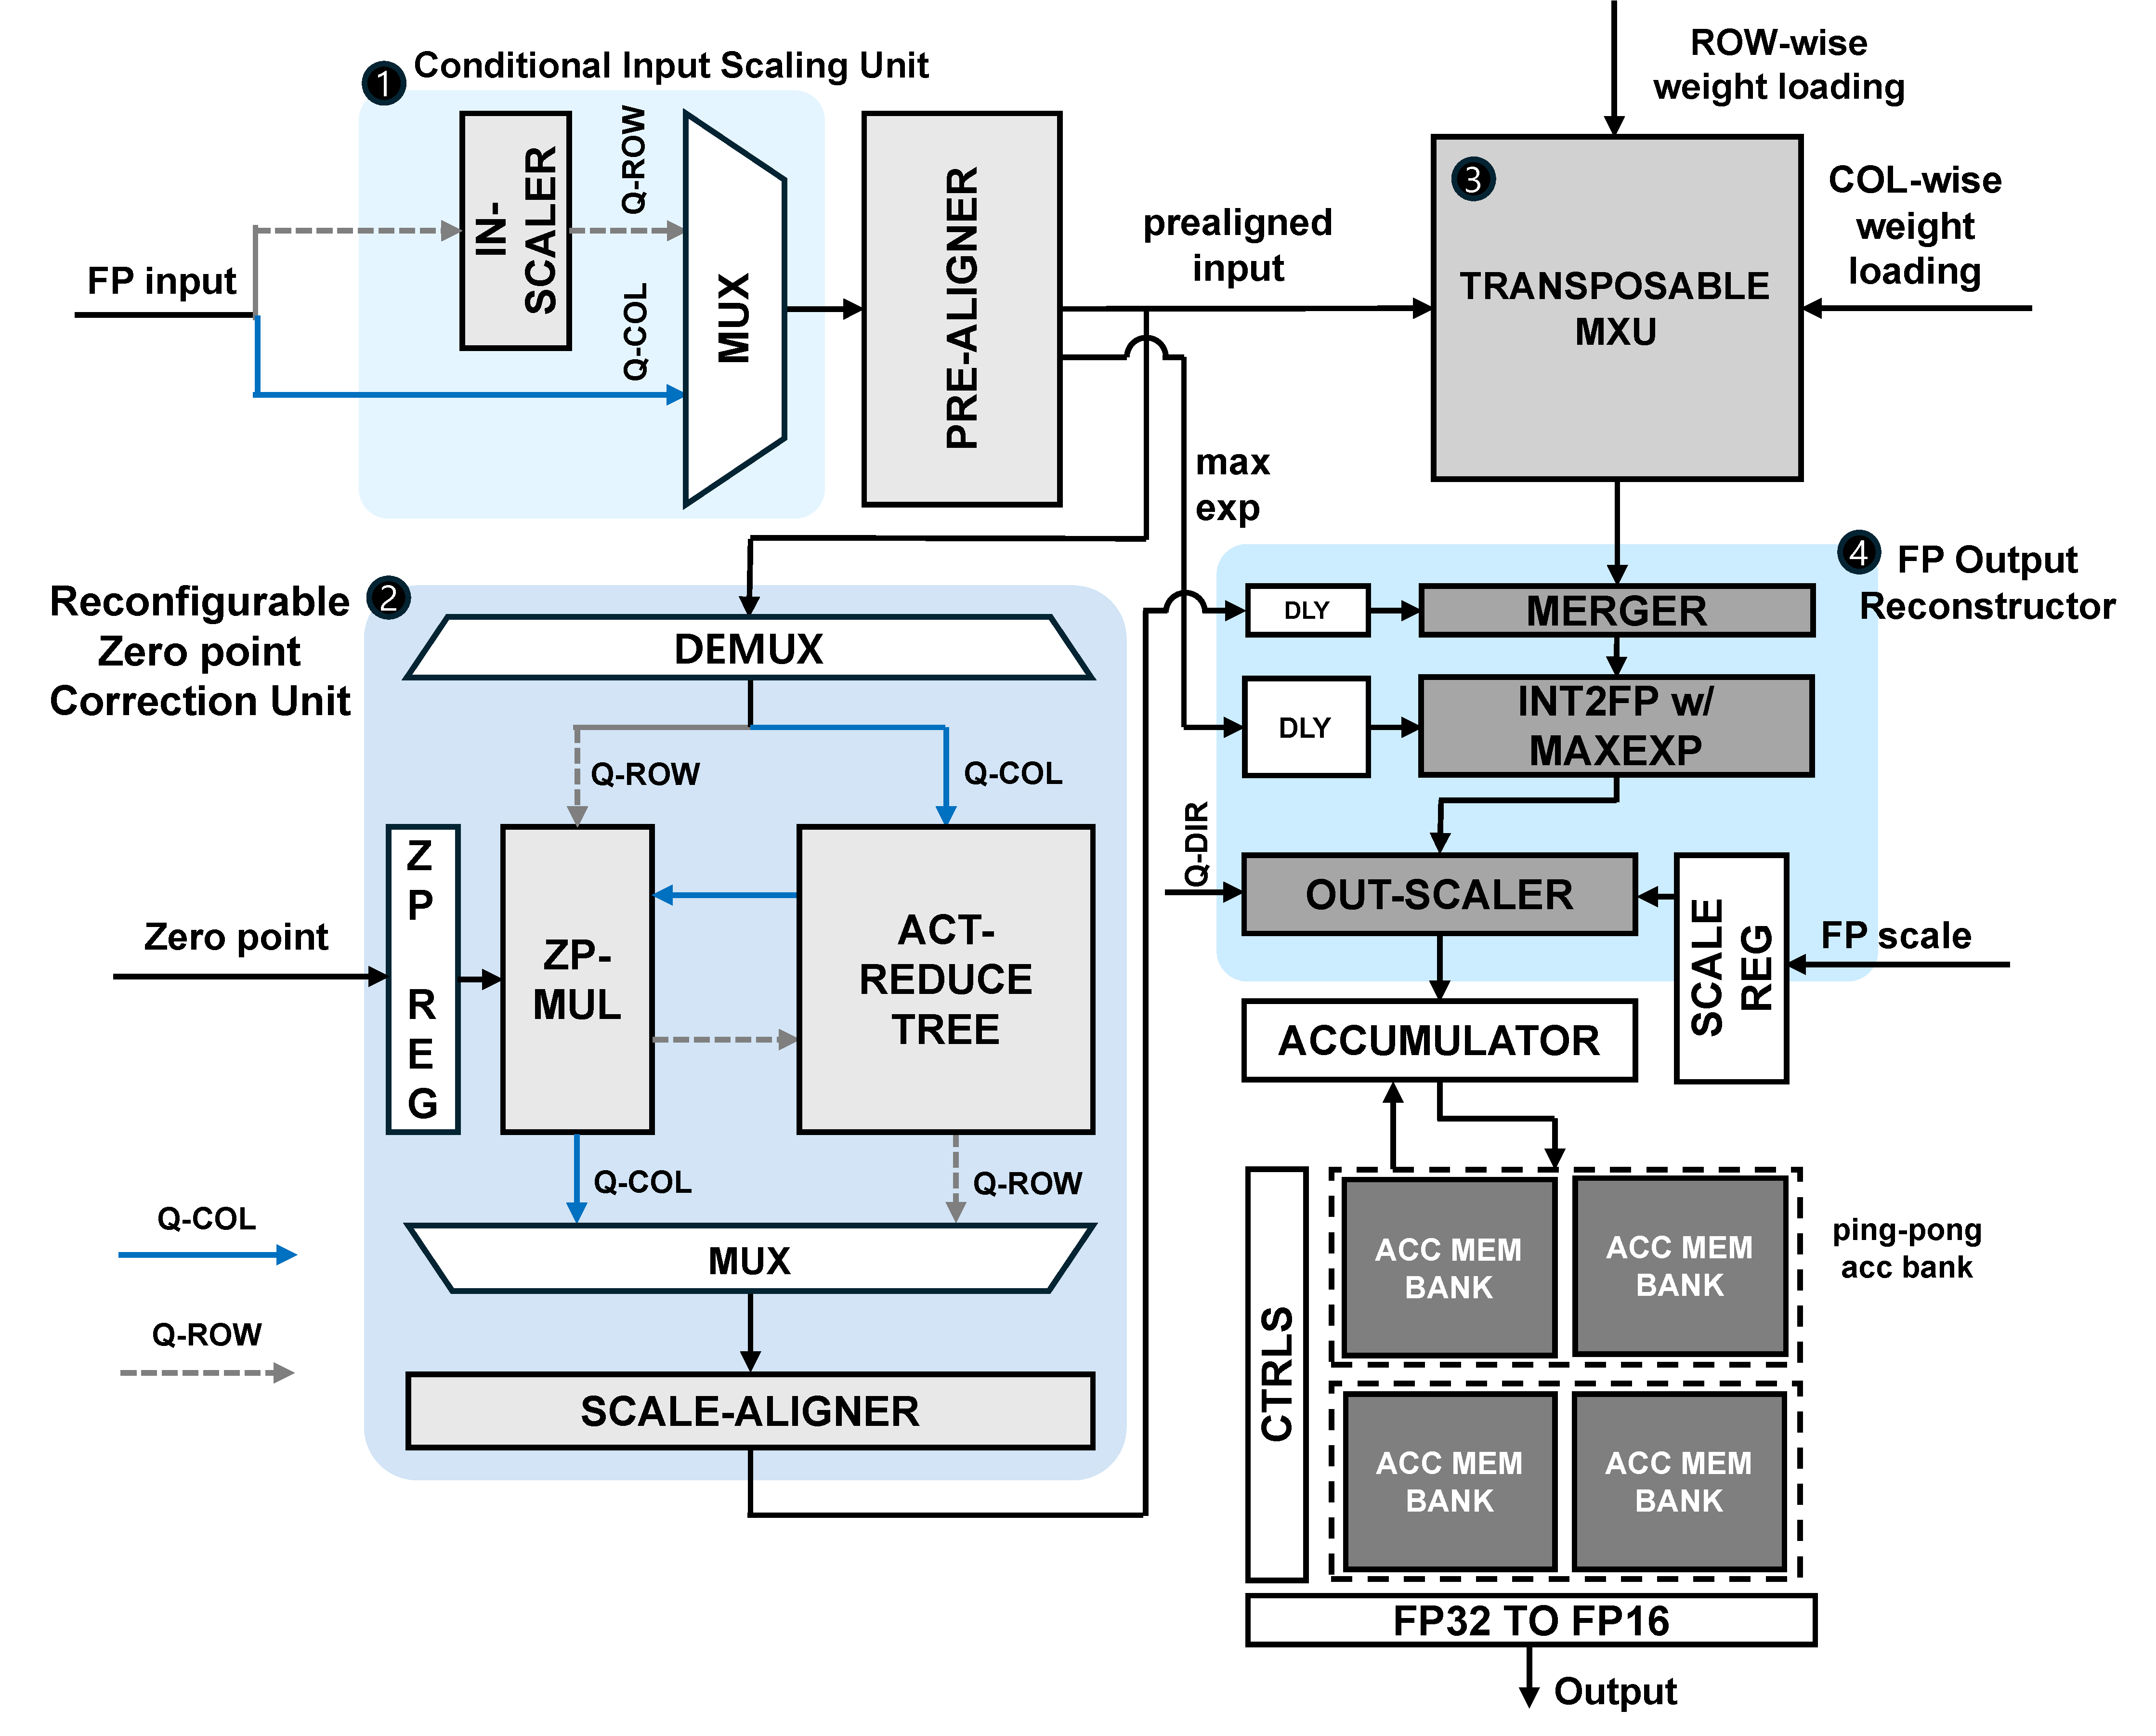
\includegraphics[width=\linewidth]{figures/gemm_engine.pdf}
    \caption{Quantization-direction-reconfigurable \fpint{} GEMM unit with a scale-folding datapath and configurable standard or transposed loading of the quantized operand.}
    \label{fig:fpint-gemm-unit}
\end{figure}

\subsection{\qcol{} Execution}
In \qcol{}, the scale and zero point are associated with the reduction group and output column. Within each group, $S^{\mathrm{COL}}_{g,n}$ and $Z^{\mathrm{COL}}_{g,n}$ are invariant with respect to the reduction index $k$, allowing output scaling to be deferred until after the integer dot product:
\begin{align}
    C^{\mathrm{COL}}_{m,n}
    &=
    \sum_g S^{\mathrm{COL}}_{g,n}
    \left(
        \sum_{k \in \mathcal{K}_g} A_{m,k} B^{\mathrm{int}}_{k,n}
        -
        Z^{\mathrm{COL}}_{g,n}
        \sum_{k \in \mathcal{K}_g} A_{m,k}
    \right).
    \label{eq:qcol-fpint}
\end{align}

Fig.~\ref{fig:fpint-gemm-unit} shows the corresponding datapath. The Conditional Input Scaling Unit ~(\blackcircletext{1}) bypasses scaling and forwards the FP input to the prealigner. After prealignment, the Reconfigurable Zero-Point Correction Unit~(\blackcircletext{2}) and the Transposable MXU~(\blackcircletext{3}) operate in parallel. The zero-point correction unit first reduces the aligned inputs and then multiplies the result by $-Z^{\mathrm{COL}}_{g,n}$, while the MXU computes the main product $\sum \hat{A}B^{\mathrm{int}}$. The FP Output Reconstructor~(\blackcircletext{4}) merges the main-product and correction paths, converts the accumulated integer result back to FP, and applies $S^{\mathrm{COL}}_{g,n}$. This organization is possible because the scale is invariant along the reduction within each group and can therefore be applied after accumulation.

\subsection{\qrow{} Scale Folding}

In \qrow{}, the scale and zero point are associated with the reduction index and output group. The direct computation is
\begin{align}
    C^{\mathrm{ROW}}_{m,n}
    &=
    \sum_k A_{m,k}
    \left(
        S^{\mathrm{ROW}}_{k,h(n)}
        \left(
            B^{\mathrm{int}}_{k,n}
            -
            Z^{\mathrm{ROW}}_{k,h(n)}
        \right)
    \right).
    \label{eq:qrow-direct}
\end{align}

Because $S^{\mathrm{ROW}}_{k,h(n)}$ changes with $k$, it cannot be factored out of the reduction, and the post-accumulation scaling used in \qcol{} is no longer valid. Likewise, the $k$-dependent zero point prevents a single correction after first reducing the inputs. A direct implementation would therefore require per-term FP dequantization followed by FP reduction, eliminating much of the efficiency of the \fpint{} datapath.

The Conditional Input Scaling Unit~(\blackcircletext{1}) avoids this FP reduction by folding the scale into the FP input before prealignment. Defining $\bar{A}^{(h)}_{m,k}=A_{m,k}S^{\mathrm{ROW}}_{k,h(n)}$, the computation becomes
\begin{align}
    C^{\mathrm{ROW}}_{m,n}
    &=
    \sum_k \bar{A}^{(h)}_{m,k}B^{\mathrm{int}}_{k,n}
    -
    \sum_k \bar{A}^{(h)}_{m,k}Z^{\mathrm{ROW}}_{k,h(n)}.
    \label{eq:qrow-fpint}
\end{align}
% ---------------------------------------------------------------------

% The scale is thus applied before the prealigner converts the FP input vector into the aligned integer representation used by the MXU. No scale operation remains in the reduction path, so both the main product and zero-point correction can be accumulated using integer arithmetic.

% Although $S^{\mathrm{ROW}}_{k,h(n)}$ depends on the output group, $h(n)$ is invariant within an MXU tile. Our 32$\times$32 MXU supports output-dimension quantization group sizes of 32, 64, and 128. If a GEMM dimension does not align with a group boundary, the kernel pads it to the next boundary so that a 32-column MXU tile never spans two output groups. All columns in a tile can therefore share the same scaled input vector. Component~\blackcircletext{1} applies one scale vector before prealignment, and the resulting input vector is reused across all 32 MXU columns. The 32$\times$32 MXU therefore requires 32 FP multipliers in the input-scaling unit rather than 1024 per-PE FP multipliers. This organization requires neither a separately scaled input for every output column nor replay of the input across columns.
% ---------------------------------------------------------------------
% +++++++++++++++++++++++++++++++++++++++++++++++++++++++++++++++++++++
The scale is applied before prealignment, so no scale operation remains in the reduction path and both the main product and zero-point correction accumulate in integer arithmetic. Although $S^{\mathrm{ROW}}_{k,h(n)}$ depends on the output group, $h(n)$ is invariant within an MXU tile: the 32$\times$32 MXU supports output-group sizes of 32, 64, and 128, and the kernel pads unaligned dimensions to the next boundary so a 32-column tile never spans two groups. All columns of a tile share one scaled input vector, letting component~\blackcircletext{1} apply the scale with 32 FP16 multipliers instead of one per PE (1024 total).
% +++++++++++++++++++++++++++++++++++++++++++++++++++++++++++++++++++++


\subsection{Reconfigurable Zero-Point Correction}
% ---------------------------------------------------------------------
% The Reconfigurable Zero-Point Correction Unit~\blackcircletext{2} implements zero-point correction in an order selected by \texttt{qdir}. We denote the prealigner output as $\hat{A}$ in \qcol{} and as $\hat{\bar{A}}$ in \qrow{}. For notational simplicity, the exponent and shift corrections are absorbed into these representations. In \qcol{}, the zero point varies only across columns within a group, so the activation sum is formed first and then multiplied by the column-specific zero point:
% \begin{align}
%     P^{\mathrm{COL}}_{m,n} &= \sum_{k \in \mathcal{T}} \hat{A}_{m,k} B^{int}_{k,n}, \\
%     R^{\mathrm{COL}}_{m} &= \sum_{k \in \mathcal{T}} \hat{A}_{m,k}, \\
%     D^{\mathrm{COL}}_{m,n} &= (-Z^{\mathrm{COL}}_{g,n}) R^{\mathrm{COL}}_{m}, \\
%     I^{\mathrm{COL}}_{m,n} &= P^{\mathrm{COL}}_{m,n} + D^{\mathrm{COL}}_{m,n} .
%     \label{eq:qcol-correction}
% \end{align}
% Thus, the correction unit uses reduce-then-multiply in \qcol{}.

% In \qrow{}, the zero point differs per reduction lane, so summing the activations first would lose track of which zero point should be multiplied. We therefore form the lane-specific zero-point product first using $\hat{\bar{A}}$ and reduce those products afterwards:
% \begin{align}
%     P^{\mathrm{ROW}}_{m,n} &= \sum_{k \in \mathcal{T}} \hat{\bar{A}}^{(h)}_{m,k} B^{int}_{k,n}, \\
%     D^{\mathrm{ROW}}_{m,h} &= \sum_{k \in \mathcal{T}} (-Z^{\mathrm{ROW}}_{k,h}) \hat{\bar{A}}^{(h)}_{m,k}, \\
%     I^{\mathrm{ROW}}_{m,n} &= P^{\mathrm{ROW}}_{m,n} + D^{\mathrm{ROW}}_{m,h} .
%     \label{eq:qrow-correction}
% \end{align}
% The same reduce tree and zero-point multiplier are used in both directions, but component~\blackcircletext{2} changes the routing from reduce-then-multiply in \qcol{} to multiply-then-reduce in \qrow{}. This change preserves the per-$k$ zero-point correction required by \qrow{} while the Transposable MXU~\blackcircletext{3} computes the main product using the same INT RHS datapath. The FP Output Reconstructor~\blackcircletext{4} then merges $P$ and $D$, converts the result back to FP, and bypasses its output scaler in \qrow{} because component~\blackcircletext{1} has already applied the scale.
% ---------------------------------------------------------------------
% +++++++++++++++++++++++++++++++++++++++++++++++++++++++++++++++++++++
The Reconfigurable Zero-Point Correction Unit~(\blackcircletext{2}) forms the zero-point term in an order selected by the quantization direction. Let $\hat{A}$ and $\hat{\bar{A}}$ denote the prealigner outputs in \qcol{} and \qrow{} (absorbing exponent and shift corrections), and let $\mathcal{T}$ be the reduction lanes in one MXU step. In \qcol{}, the zero point is constant across $\mathcal{T}$, so the unit reduces the inputs first and multiplies once by the column zero point; in \qrow{}, it differs per lane, so the unit forms the lane-wise products first and reduces them afterward:
\begin{align}
    D^{\mathrm{COL}}_{m,n}
    &=
    \left(-Z^{\mathrm{COL}}_{g,n}\right)
    \sum_{k \in \mathcal{T}} \hat{A}_{m,k},
    \\
    D^{\mathrm{ROW}}_{m,h}
    &=
    \sum_{k \in \mathcal{T}}
    \left(-Z^{\mathrm{ROW}}_{k,h}\right)
    \hat{\bar{A}}^{(h)}_{m,k}.
\end{align}
The Transposable MXU~(\blackcircletext{3}) computes the main product $P_{m,n}=\sum_{k \in \mathcal{T}} \hat{A}_{m,k}B^{\mathrm{int}}_{k,n}$ on the same INT datapath, and the FP Output Reconstructor~(\blackcircletext{4}) adds $P$ and $D$ before converting back to FP. The same reduction tree and zero-point multiplier serve both modes; component~\blackcircletext{2} only reroutes from reduce-then-multiply (\qcol{}) to multiply-then-reduce (\qrow{}). The output scaler is enabled in \qcol{} and bypassed in \qrow{}, where component~\blackcircletext{1} has already applied the scale.
% +++++++++++++++++++++++++++++++++++++++++++++++++++++++++++++++++++++

\subsection{Configurable Operand Loading and Accumulation}

Attention changes not only the quantization direction but also the logical orientation of the quantized operand. Linear GEMMs and PV consume $B^{\mathrm{int}}$ in its standard orientation, whereas QK$^T$ consumes the K operand in transposed form. To support both cases without a separate transpose kernel, the Transposable MXU~(\blackcircletext{3}) provides separate row-wise and column-wise load paths for the same physical array. 
%The load orientation is configured independently of \texttt{qdir}: \texttt{qdir} selects the scaling and zero-point-correction datapath, while the load-orientation field determines how $B^{\mathrm{int}}$ is delivered to the MXU. 
The upper-level architecture configures the quantization direction and operand loading direction for each linear, QK$^T$, or PV kernel while sharing one \fpint{} array across all operations.

%The \texttt{DLY} block in Figure~\ref{fig:fpint-gemm-unit} is an Flip-Flop (FF)-based delay element that equalizes the pipeline latency of the main-product and correction paths. It ensures that the \texttt{merger} and accumulator stage receive cycle-aligned partial results. The \texttt{ACC MEM BANK} stores partial sums using two single-port SRAM banks scheduled in a one-cycle-skewed ping-pong manner. While one bank is read in a cycle, the other is written, allowing the pair to behave as a logically dual-port accumulator memory without requiring a true dual-port SRAM.
%The \texttt{DLY} block in Figure~\ref{fig:fpint-gemm-unit} aligns the pipeline latencies of the main-product and correction paths for cycle-synchronous merging and accumulation. The \texttt{ACC MEM BANK} uses two single-port SRAM banks in a one-cycle-skewed ping-pong scheme, providing logical dual-port operation by reading one bank while writing the other.

By supporting \qcol{} and \qrow{} together with standard and transposed operand loading, the proposed MXU executes both QK$^T$ and PV as native \fpint{} GEMMs alongside the linear layers. This eliminates the FP fallback that would otherwise leave quantized attention as the long-context bottleneck.





\iffalse
\section[Native FP-INT Attention Support]{Native \texorpdfstring{\fpint{}}{FP-INT} Attention Support}

As discussed in Section~\ref{sec:sys_gap}, native \fpint{} attention requires more than an MXU that multiplies one FP operand by one INT operand. The key issue is whether the quantization metadata changes along the GEMM reduction direction. If one scale and zero point are shared across the values being reduced, the MXU can first compute the INT dot product and apply dequantization afterward. This is the common case in GEMMs in linear layers, where metadata is fixed by output channel or group. 
%In KV-cache quantization, however, QK$^T$ and PV map token and channel axes to different GEMM directions. 
In KV-cache quantization, however, the key and value caches can each be quantized along either the token or channel dimension, with the selected quantization axes varying across frameworks.
%A scheme that keeps metadata outside the reduction direction in one attention GEMM can place different scales along the reduction direction in the other. 
In that case, each product must be dequantized before accumulation, so a conventional \fpint{} MXU needs per-term FP multiplication and FP reduction or falls back to the FP attention path.

To address this, we propose a \fpint{} MXU that independently reconfigures the RHS quantization direction between \qcol{} and \qrow{} and separately configures the RHS load direction. The \texttt{qdir} field selects where the \fpint{} GEMM applies the scale and the zero point. In the following, $A$ is the FP input operand, $B^{int}$ is the INT RHS operand, $G_K$ and $G_N$ are the quantization group sizes along the reduction and output dimensions, $g(k)=\lfloor k/G_K \rfloor$, and $h(n)=\lfloor n/G_N \rfloor$.

The same prealigner is shared by \qcol{} and \qrow{}. We follow the numerical accuracy preserving prealignment scheme of FIGNA~\cite{figna} and represent each FP16 input using a 31 bit signed aligned mantissa before integer multiplication and reduction. The subsequent integer accumulation and conversion back to FP also follow FIGNA.

In \qcol{}, the scale and the zero point are bound to the reduction group and the output column. Within a group, $S^{\mathrm{COL}}_{g,n}$ and $Z^{\mathrm{COL}}_{g,n}$ are invariant in the reduction index $k$, so output scaling can be deferred to the end of the dot product:
\begin{align}
    C^{\mathrm{COL}}_{m,n}
    &=
    \sum_g S^{\mathrm{COL}}_{g,n}
    \left(
        \sum_{k \in \mathcal{K}_g} A_{m,k} B^{int}_{k,n}
        -
        Z^{\mathrm{COL}}_{g,n} \sum_{k \in \mathcal{K}_g} A_{m,k}
    \right) .
    \label{eq:qcol-fpint}
\end{align}
Fig.~\ref{fig:fpint-gemm-unit} shows how this \qcol{} computation is implemented. The Conditional Input Scaling Unit~\blackcircletext{1} selects the unscaled activation and forwards it to the prealigner. After prealignment, the Reconfigurable Zero-Point Correction Unit~\blackcircletext{2} and the Transposable MXU~\blackcircletext{3} operate in parallel. The former reduces the aligned activations and then multiplies the result by $-Z^{\mathrm{COL}}_{g,n}$, while the latter computes the main product $\sum \hat{A} B^{int}$. The FP Output Reconstructor~\blackcircletext{4} merges the correction and main-product paths, converts the result back to FP, and applies $S^{\mathrm{COL}}_{g,n}$. This dataflow is possible because the scale remains stationary along the output lane.

In \qrow{}, by contrast, the scale and the zero point are bound to the reduction index and the output group. The direct \qrow{} computation is
\begin{align}
    C^{\mathrm{ROW}}_{m,n}
    &=
    \sum_k A_{m,k}
    \left(
        S^{\mathrm{ROW}}_{k,h(n)} \cdot
        (B^{int}_{k,n} - Z^{\mathrm{ROW}}_{k,h(n)})
    \right) .
    \label{eq:qrow-direct}
\end{align}
Because $S^{\mathrm{ROW}}_{k,h(n)}$ changes with $k$, it cannot be factored out of the reduction, and \qcol{} scaling after accumulation is no longer valid. Likewise, the $k$-dependent zero point prevents a single correction after first reducing the activations. A direct datapath would therefore need to dequantize each term before accumulation, which is inefficient.

The \qrow{} datapath does not eliminate the scale multiplication required for each reduction term.
Instead, the Conditional Input Scaling Unit~\blackcircletext{1} moves this multiplication from RHS dequantization to the FP input before prealignment.
Define $\bar{A}^{(h)}_{m,k}=A_{m,k}S^{\mathrm{ROW}}_{k,h(n)}$. The \qrow{} computation then becomes
\begin{align}
    C^{\mathrm{ROW}}_{m,n}
    &=
    \sum_k \bar{A}^{(h)}_{m,k} B^{int}_{k,n}
    -
    \sum_k \bar{A}^{(h)}_{m,k} Z^{\mathrm{ROW}}_{k,h(n)},
    \label{eq:qrow-fpint}
\end{align}
The scale is now absorbed into $\bar{A}$ before the prealigner converts the FP vector into the aligned integer representation used by the MXU.
The downstream datapath therefore does not consume scale metadata that varies along the reduction dimension.
Equivalently, every reduction term after prealignment has an effective scale of one.
This does not mean that the scale metadata is rewritten to one. It means that the scale has already been applied to the FP input and no additional scale operation remains in the reduction path.
The main product and zero point correction can therefore use integer reduction.
The remaining zero point term is handled by the correction path selected by \texttt{qdir} as described below.
Although $S^{\mathrm{ROW}}_{k,h(n)}$ is indexed by the output group, $h(n)$ is invariant within an MXU tile.
Our 32$\times$32 MXU supports quantization group sizes of 32, 64, and 128 along the output dimension.
When a GEMM dimension does not align with a quantization group boundary, the kernel pads it to the next boundary, so a 32 column MXU tile never spans two output groups.
Consequently, all columns in an MXU tile use the same scale vector.
The input scaler in component~\blackcircletext{1} applies this scale vector before prealignment, and the resulting activation vector is reused by all 32 MXU columns.
For our 32$\times$32 MXU, component~\blackcircletext{1} contains 32 FP multipliers rather than 1024 per-PE multipliers.
This organization requires neither a separate scaled activation for each column nor activation replay across columns.

The Reconfigurable Zero-Point Correction Unit~\blackcircletext{2} implements zero-point correction in an order selected by \texttt{qdir}. We denote the prealigner output as $\hat{A}$ in \qcol{} and as $\hat{\bar{A}}$ in \qrow{}. For notational simplicity, the exponent and shift corrections are absorbed into these representations. In \qcol{}, the zero point varies only across columns within a group, so the activation sum is formed first and then multiplied by the column-specific zero point:
\begin{align}
    P^{\mathrm{COL}}_{m,n} &= \sum_{k \in \mathcal{T}} \hat{A}_{m,k} B^{int}_{k,n}, \\
    R^{\mathrm{COL}}_{m} &= \sum_{k \in \mathcal{T}} \hat{A}_{m,k}, \\
    D^{\mathrm{COL}}_{m,n} &= (-Z^{\mathrm{COL}}_{g,n}) R^{\mathrm{COL}}_{m}, \\
    I^{\mathrm{COL}}_{m,n} &= P^{\mathrm{COL}}_{m,n} + D^{\mathrm{COL}}_{m,n} .
    \label{eq:qcol-correction}
\end{align}
Thus, the correction unit uses reduce-then-multiply in \qcol{}.

In \qrow{}, the zero point differs per reduction lane, so summing the activations first would lose track of which zero point should be multiplied. We therefore form the lane-specific zero-point product first using $\hat{\bar{A}}$ and reduce those products afterwards:
\begin{align}
    P^{\mathrm{ROW}}_{m,n} &= \sum_{k \in \mathcal{T}} \hat{\bar{A}}^{(h)}_{m,k} B^{int}_{k,n}, \\
    D^{\mathrm{ROW}}_{m,h} &= \sum_{k \in \mathcal{T}} (-Z^{\mathrm{ROW}}_{k,h}) \hat{\bar{A}}^{(h)}_{m,k}, \\
    I^{\mathrm{ROW}}_{m,n} &= P^{\mathrm{ROW}}_{m,n} + D^{\mathrm{ROW}}_{m,h} .
    \label{eq:qrow-correction}
\end{align}
The same reduce tree and zero-point multiplier are used in both directions, but component~\blackcircletext{2} changes the routing from reduce-then-multiply in \qcol{} to multiply-then-reduce in \qrow{}. This change preserves the per-$k$ zero-point correction required by \qrow{} while the Transposable MXU~\blackcircletext{3} computes the main product using the same INT RHS datapath. The FP Output Reconstructor~\blackcircletext{4} then merges $P$ and $D$, converts the result back to FP, and bypasses its output scaler in \qrow{} because component~\blackcircletext{1} has already applied the scale.

Attention changes not only the quantization direction but also the logical orientation of the RHS. PV and linear GEMMs consume the RHS tile in the standard orientation, whereas QK$^T$ must feed the K tile to the MXU in transposed form. To support this, the Transposable MXU~\blackcircletext{3} duplicates the RHS load network so that the same array supports both row-wise and column-wise loading. The transpose is thus absorbed into a load-time configuration rather than handled by a separate memory-transform kernel. As shown in Fig.~\ref{fig:fpint-gemm-unit}, \texttt{qdir} configures the scaling and zero-point-correction datapath, while the load direction independently determines how the RHS matrix is delivered to the weight input of the MXU. The upper-level architecture only needs to set \texttt{qdir} and load direction for each linear, QK$^T$, or PV kernel, while the physical \fpint{} MXU array is shared across all paths.

%The \texttt{DLY} block in Figure~\ref{fig:fpint-gemm-unit} is an FF-based delay element that matches the pipeline latency between the main product path and the correction path, both of which vary with \texttt{qdir} and load direction. 
The \texttt{DLY} block in Fig.~\ref{fig:fpint-gemm-unit} is an FF-based delay element that matches the pipeline latency between the main product path and the correction path. 
With \texttt{DLY}, the \texttt{merger} and the accumulator stage receive cycle-aligned partial results. The \texttt{ACC MEM BANK} is dedicated storage for partial-sum accumulation. Instead of a true dual-port SRAM, it uses two single-port SRAM banks scheduled in a 1-cycle skewed ping-pong fashion: while one bank is read in a given cycle, the other is written, constraining the dataflow so that the two single-port banks behave as a logically dual-port accumulator bank.

\begin{figure}[t]
    \centering
    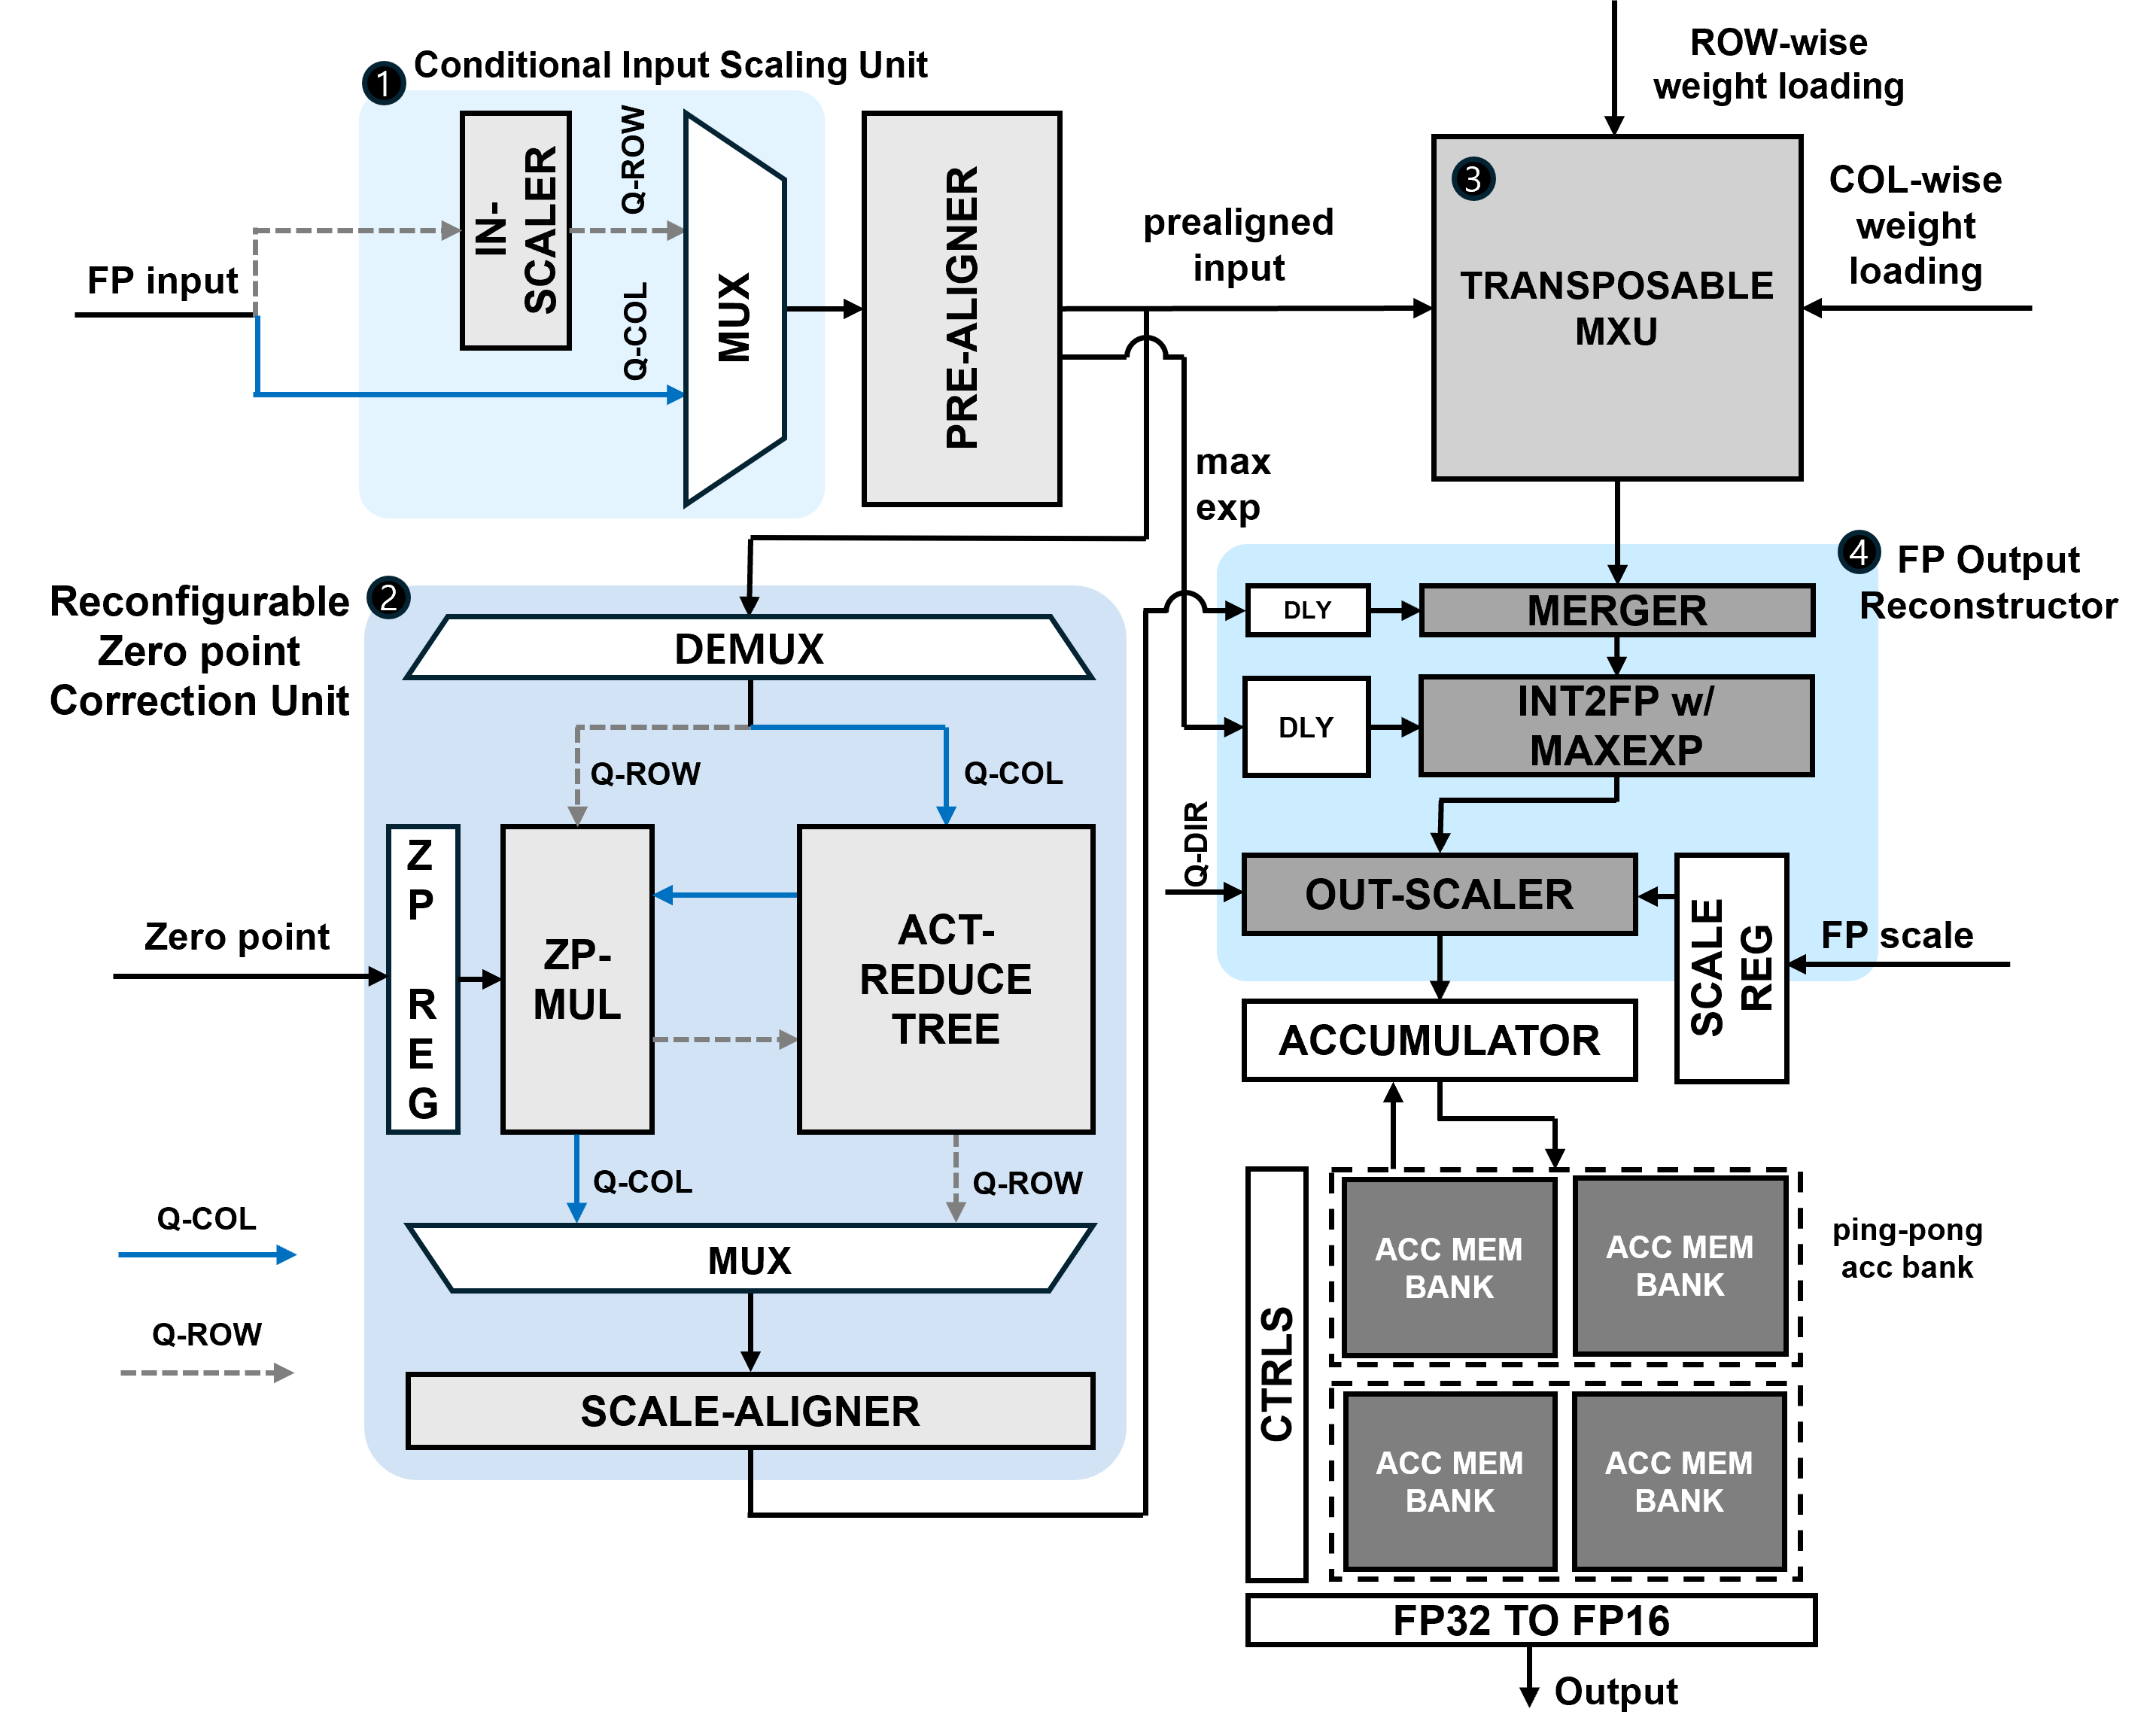
\includegraphics[width=0.92\linewidth]{figures/gemm_engine.png}
    \caption{RHS quantization direction reconfigurable \fpint{} GEMM unit with scale folding datapath and dual RHS load paths.}
    \label{fig:fpint-gemm-unit}
\end{figure}

The key effect is eliminating FP fallback in quantized attention. A linear-only \fpint{} design leaves attention as the long-context bottleneck, while the proposed MXU executes both QK$^T$ and PV as native \fpint{} GEMMs alongside the linear layers.
\fi

\section[Tensor Memory System for Sustained FP-INT Utilization]{Tensor Memory System for Sustained \texorpdfstring{\fpint{}}{FP-INT} Utilization}
\label{sec:memory-system}

An \fpint{} MXU can provide more MACs than an FP$\times$FP Tensor Core within the same area and energy budget, but this higher compute density is useful only if operands and partial sums can be supplied at a matching rate. Scaling the conventional register-file, local-memory, and cache paths would require additional ports, banks, arbitration, and wiring, eroding the density advantage of the \fpint{} array. \ours{} therefore isolates regular high-bandwidth tensor transfers from the general-purpose SIMT memory path rather than attaching a larger MXU to the existing memory hierarchy.

\subsection{Partitioned On-Chip Tensor Storage}

% General-purpose local memory must support conventional load/store operations, inter-thread communication, and irregular accesses from scalar and vector kernels. GEMM operands, in contrast, follow fixed tile shapes and predictable access orders, making banked bandwidth more important than arbitrary access flexibility. \ours{} therefore partitions on-chip SRAM into general-purpose local memory, MXU-dedicated tensor memory (\mbox{TMEM}), and dedicated accumulator memory (\mbox{ACC MEM}). Local memory preserves the SIMT programming model, while TMEM and ACC MEM scale their bank counts and data widths under more restricted access patterns.
% Storing wider partial sums in a dedicated ACC MEM, separate from input and weight traffic, removes read-modify-write interference and prevents ready-signal back-pressure from stalling the deeply pipelined GEMM datapath.
Local memory must serve conventional load/store, inter-thread communication, and irregular scalar/vector accesses, whereas GEMM operands follow fixed tile shapes and predictable orders, making banked bandwidth matter more than access flexibility. \ours{} therefore partitions on-chip SRAM into general-purpose local memory, MXU-dedicated tensor memory (\mbox{TMEM}), and accumulator memory (\mbox{ACC MEM}): local memory preserves the SIMT programming model, while TMEM and ACC MEM scale bank counts and data widths under restricted access patterns. Keeping wider partial sums in ACC MEM, separate from input and weight traffic, removes read-modify-write interference and prevents back-pressure from stalling the deeply pipelined GEMM datapath.

\begin{figure}[t]
    \centering
    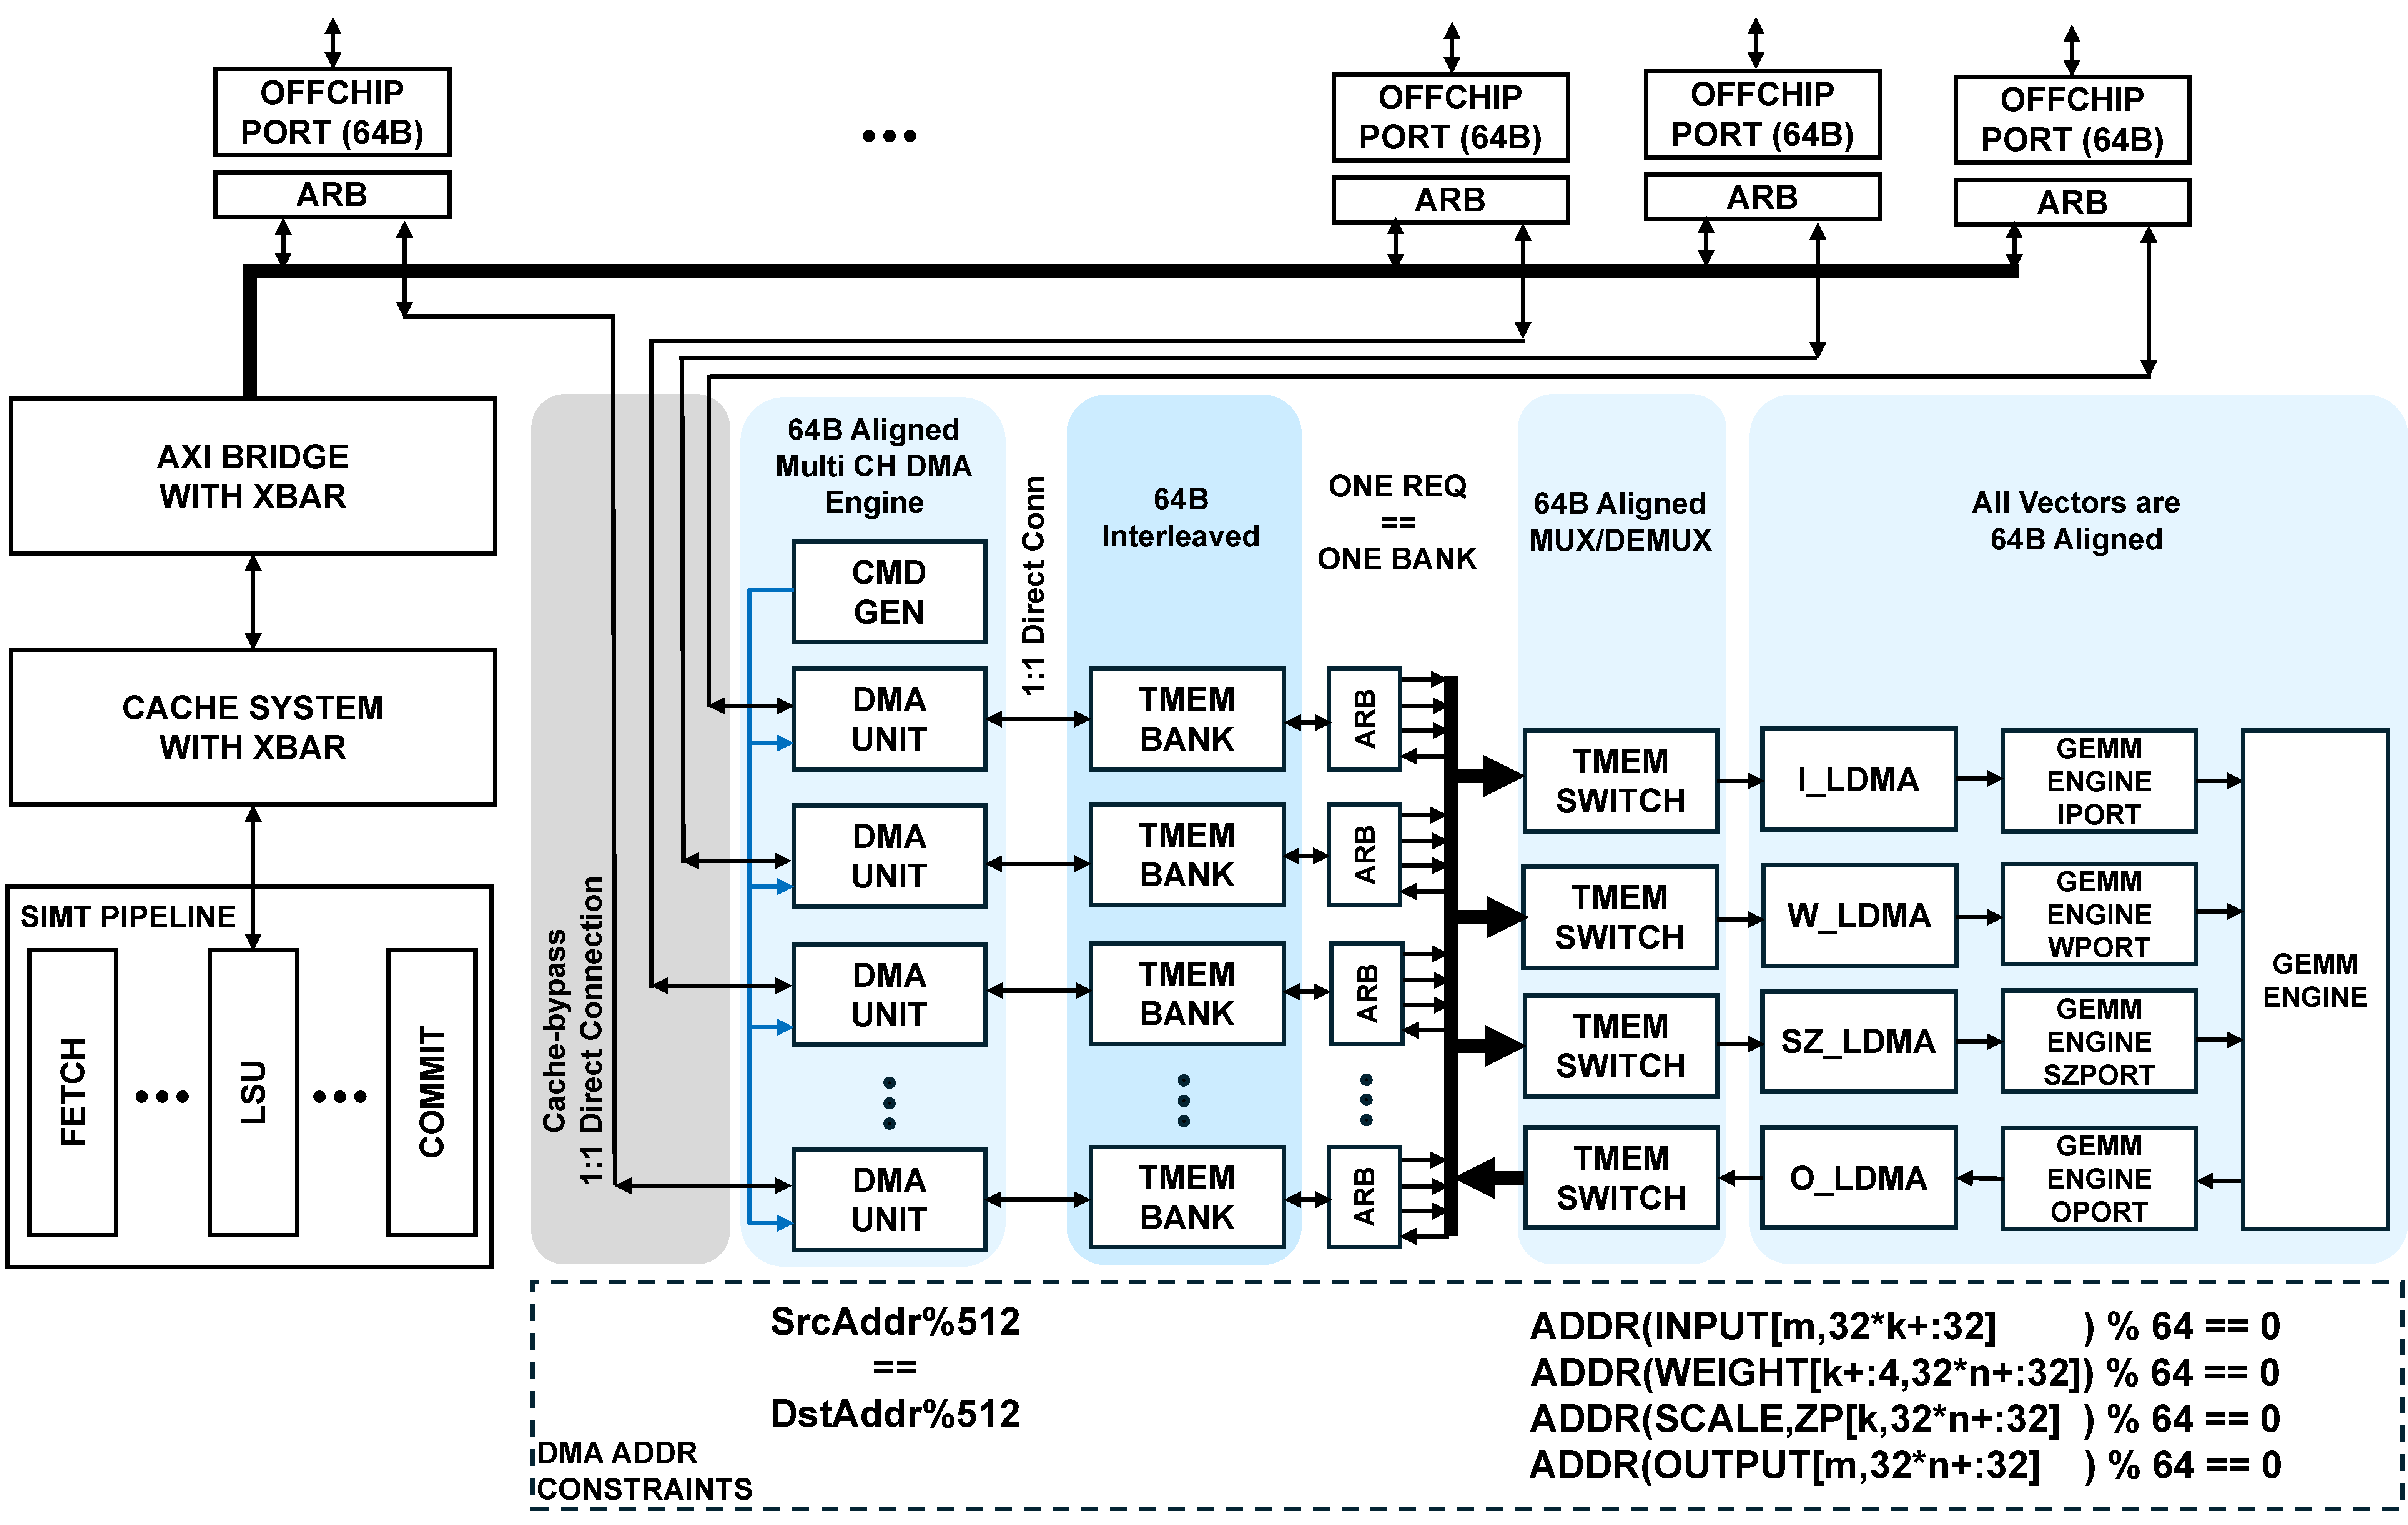
\includegraphics[width=\linewidth]{figures/mem_system.pdf}
    \caption{Tensor memory system with partitioned on-chip storage, interleaved connectivity, and cache-bypassed data movement.}
    \label{fig:memory-system}
\end{figure}

\subsection{Interleaved and Aligned Tensor Data Path}

A full crossbar between HBM pseudo-channels and TMEM banks would provide unrestricted connectivity, but its multiplexing, arbitration, and routing costs grow rapidly with the number and width of its ports.
%\ours{} instead uses either one-to-one or interleaved mappings for both the HBM--TMEM and TMEM--MXU paths. 
\ours{} instead uses a one-to-one or interleaved mapping at the HBM--TMEM boundary and restricted wide-word mux/demux paths at the TMEM--MXU boundary.
Fig.~\ref{fig:memory-system} illustrates a configuration with a 64\,B HBM/TMEM transfer width, eight HBM pseudo-channels, eight TMEM banks, and FP16 inputs. Here, $R_{\mathrm{MXU}}$ denotes the MXU row dimension, or equivalently the number of reduction lanes consumed per input slice.

% ---------------------------------------------------------------------
% HBM--TMEM and TMEM--MXU boundaries impose different software-visible constraints. At the HBM--TMEM boundary, the HBM pseudo-channel and TMEM bank selected by the two addresses must be physically connected, and both DMA addresses must be aligned to the $DW$-byte transfer granularity. Consider two memory endpoints with $N_L$ and $N_S$ ports, where $N_L \geq N_S$. For a byte address $A_E$ at memory endpoint $E$, low-order interleaving selects
% \begin{equation}
%     b_E\left(A_E\right)
%     =
%     \left\lfloor
%         \frac{A_E}{DW}
%     \right\rfloor
%     \bmod N_E .
%     \label{eq:interleaved_endpoint_index}
% \end{equation}
% The fixed interconnect maps port $j$ of the larger endpoint to port $j \bmod N_S$ of the smaller endpoint. Consequently, a transfer between addresses $A_L$ and $A_S$ is possible only if
% \begin{equation}
%     b_S\left(A_S\right)
%     =
%     b_L\left(A_L\right)
%     \bmod N_S .
%     \label{eq:general_interleaved_constraint}
% \end{equation}
% Independently, the aligned-only DMA requires
% \begin{equation}
%     A_L \bmod DW
%     =
%     A_S \bmod DW
%     =
%     0 .
%     \label{eq:aligned_dma_constraint}
% \end{equation}
% Equal endpoint counts give a 1:1 mapping; unequal counts give the deterministic interleaved mapping in Eq.~\ref{eq:general_interleaved_constraint}. For example, a 4-to-8 connection maps endpoint $i$ on the eight-port side to endpoint $i \bmod 4$ on the four-port side. %We use neither address hashing nor XOR-based bank selection.

% At the HBM--TMEM boundary, $N_L$ and $N_S$ are the larger and smaller of the pseudo-channel count $N_{\mathrm{pc}}$ and TMEM-bank count $N_{\mathrm{tmem}}$, respectively. Eqs.~\ref{eq:general_interleaved_constraint} and~\ref{eq:aligned_dma_constraint} therefore determine whether data at an HBM address can be placed at a given TMEM address.

% At the TMEM--MXU boundary, each fixed GEMM port can select any TMEM bank, so there is no bank-to-port reachability constraint. The restriction instead comes from omitting cross-bank realignment: every vector must begin at a 64\,B boundary so that it occupies exactly one TMEM bank word. Let $\mathcal{G}=\{I,W,SZ,O\}$ and let $V_g$ denote the vector width of port $g$. In \ours{},
% \begin{equation}
%     V_I=V_W=V_{SZ}=V_O=64\,\mathrm{B}.
%     \label{eq:gemm_vector_width}
% \end{equation}
% The first element of every transferred tensor vector must therefore satisfy
% \begin{equation}
%     \operatorname{Addr}_{\mathrm{TMEM}}
%     \left(T_g[v]\right)
%     \equiv 0
%     \pmod{V_g},
%     \qquad g\in\mathcal{G}.
%     \label{eq:tmem_gemm_vector_constraint}
% \end{equation}
% For example, the input port consumes $I[m,R_{\mathrm{MXU}}k:R_{\mathrm{MXU}}(k+1)-1]$. With FP16 input and $R_{\mathrm{MXU}}=32$, $V_I=\operatorname{sizeof}(I)R_{\mathrm{MXU}}=64\,\mathrm{B}$, so the first element $I[m,R_{\mathrm{MXU}}k]$ must satisfy Eq.~\ref{eq:tmem_gemm_vector_constraint}. The output port reverses the transfer direction but obeys the same alignment condition. 
% Although these address constraints would be restrictive for arbitrary copies, regular GEMM tiles can satisfy them through aligned allocation and layout transformation, as described in Section~\ref{sec:runtime-section}.
% ---------------------------------------------------------------------
% +++++++++++++++++++++++++++++++++++++++++++++++++++++++++++++++++++++
The two boundaries impose different software-visible constraints. At the HBM--TMEM boundary, the selected HBM pseudo-channel and TMEM bank must be physically connected and both DMA addresses must be aligned to the $DW$-byte transfer granularity. For two endpoints with $N_L \geq N_S$ ports under low-order interleaving, a byte address $A_E$ selects port $b_E(A_E)=\lfloor A_E/DW \rfloor \bmod N_E$, and the interconnect maps port $j$ of the larger endpoint to port $j \bmod N_S$ of the smaller one. A transfer between $A_L$ and $A_S$ is therefore possible only if
\begin{equation}
    b_S\left(A_S\right)
    =
    b_L\left(A_L\right)
    \bmod N_S ,
    \label{eq:general_interleaved_constraint}
\end{equation}
while the aligned-only DMA independently requires
\begin{equation}
    A_L \bmod DW
    =
    A_S \bmod DW
    =
    0 .
    \label{eq:aligned_dma_constraint}
\end{equation}
Here $N_L$ and $N_S$ are the larger and smaller of the pseudo-channel count $N_{\mathrm{pc}}$ and TMEM-bank count $N_{\mathrm{tmem}}$, so \eqref{eq:general_interleaved_constraint} and \eqref{eq:aligned_dma_constraint} determine whether an HBM address can be placed at a given TMEM address. A 4-to-8 connection, for example, maps eight-port endpoint $i$ to four-port endpoint $i \bmod 4$.

At the TMEM--MXU boundary, each GEMM port can select any TMEM bank, so the only restriction is that omitting cross-bank realignment forces every vector to begin at a 64\,B boundary and occupy exactly one bank word. With $\mathcal{G}=\{I,W,SZ,O\}$ and every port width $V_g=64\,\mathrm{B}$, the first element of each transferred vector must satisfy
\begin{equation}
    \operatorname{Addr}_{\mathrm{TMEM}}
    \left(T_g[v]\right)
    \equiv 0
    \pmod{V_g},
    \qquad g\in\mathcal{G}.
    \label{eq:tmem_gemm_vector_constraint}
\end{equation}
For instance, the input port consumes $I[m,R_{\mathrm{MXU}}k:R_{\mathrm{MXU}}(k+1)-1]$, which for FP16 input and $R_{\mathrm{MXU}}=32$ gives $V_I=64\,\mathrm{B}$; the output port obeys the same condition in reverse. Regular GEMM tiles satisfy these constraints through aligned allocation and layout transformation (Section~\ref{sec:runtime-section}).
% +++++++++++++++++++++++++++++++++++++++++++++++++++++++++++++++++++++

\subsection{Specialized Tensor DMA Engines} 

\ours{} uses two specialized DMA subsystems for tensor movement, one across the HBM--TMEM boundary which we refer to as the Tile DMA (T-DMA), and one across the TMEM--GEMM-engine boundary which we refer to as the GEMM Engine DMA (G-DMA).

% ---------------------------------------------------------------------
% \textbf{Tile DMA (T-DMA).} The T-DMA moves tensor tiles directly between HBM pseudo-channels and TMEM banks through the fixed one-to-one or interleaved interconnect while bypassing the cache hierarchy. It intentionally supports only requests aligned to the $DW$-byte aligned requests. Supporting arbitrary byte offsets on this wide datapath would require either a $DW$-byte-wide barrel shifter for single-cycle realignment or a multi-cycle realignment path with additional staging buffers. The latter would increase transfer latency and require more in-flight requests to sustain bandwidth. Restricting the interface to aligned requests avoids the datapath, buffering, and control required solely for realignment. Section~\ref{sec:runtime-section} describes how tile-major layouts and alignment-aware allocation satisfy this restriction. Cache bypass prevents tensor traffic from contending with cache banks, local memory, and SIMT load/store traffic. Because the path is non-coherent with the cache hierarchy, the runtime ensures visibility through producer fences, result-tile completion polling, and cache management at kernel boundaries. 

% \textbf{GEMM Engine DMA (G-DMA).} The G-DMA consists of four independent engines associated with the fixed 64\,B input (\texttt{I}), weight (\texttt{W}), scale/zero-point (\texttt{SZ}), and output (\texttt{O}) ports. The \texttt{I}, \texttt{W}, and \texttt{SZ} engines read input, weight, and scale/zero-point data from TMEM, respectively, whereas the \texttt{O} engine writes GEMM results back to TMEM. Each engine can select any TMEM bank and transfers one aligned 64\,B port word at a time. For 4-bit weights and a 32$\times$32 MXU, each \texttt{W}-port transfer supplies 128 weights, corresponding to four 32-element weight rows. Unlike the approximately ten-cycle local-memory path in the baseline GPU, TMEM is tightly coupled to the G-DMA and provides a short and deterministic response latency. The G-DMA therefore requires fewer outstanding requests and shallower request queues to sustain the fixed bandwidth of each port. The four engines operate independently, allowing input, weight, and scale/zero-point delivery to overlap with result writeback when their TMEM accesses do not conflict. 

% Overall, the aligned-only T-DMA removes wide realignment hardware from the HBM--TMEM path, while the low-latency TMEM interface keeps the G-DMA request machinery shallow. Together with fixed interconnects and cache bypass, these specialized DMA engines sustain operand delivery without proportionally scaling the general-purpose memory fabric.
% ---------------------------------------------------------------------
% +++++++++++++++++++++++++++++++++++++++++++++++++++++++++++++++++++++
\textbf{Tile DMA (T-DMA).} The T-DMA moves tensor tiles directly between HBM pseudo-channels and TMEM banks through the interleaved interconnect while bypassing the cache. It supports only $DW$-byte-aligned requests: arbitrary byte offsets would require a wide barrel shifter or a multi-cycle realignment path with extra staging buffers, increasing latency and outstanding-request pressure. Tile-major layouts satisfy this restriction (Section~\ref{sec:runtime-section}). Cache bypass keeps tensor traffic off the cache, local-memory, and SIMT load/store paths; because this path is non-coherent, the runtime ensures visibility through producer fences, result-tile completion polling, and cache management at kernel boundaries.

\textbf{GEMM Engine DMA (G-DMA).} Four independent engines drive the fixed 64\,B input (\texttt{I}), weight (\texttt{W}), scale/zero-point (\texttt{SZ}), and output (\texttt{O}) ports; \texttt{I}/\texttt{W}/\texttt{SZ} read operands from TMEM and \texttt{O} writes results back. Each engine selects any TMEM bank and moves one aligned 64\,B word per transfer, so with 4-bit weights and a 32$\times$32 MXU each \texttt{W} transfer supplies 128 weights (four 32-element rows). Because TMEM is tightly coupled and provides a 1-cycle access latency, compared with the roughly 20-cycle access latency of the baseline local-memory path, the G-DMA sustains its port bandwidth with few outstanding requests and shallow queues, and the four engines overlap operand delivery with result writeback when their accesses do not conflict.
% +++++++++++++++++++++++++++++++++++++++++++++++++++++++++++++++++++++

%\subsection{Cache-Bypassed Descriptor-Driven Tensor Movement}

%Tensor transfers between HBM and TMEM bypass the cache hierarchy. Routing this traffic through the cache would place it on paths shared with cache banks, local memory, and SIMT load/store requests, reintroducing the arbitration and port pressure that the dedicated tensor path is intended to avoid. \ours{} instead transfers tensor tiles directly between HBM pseudo-channels and TMEM banks, reducing cache pollution and contention with vector kernels.

%Because this path lies outside the coherent cache protocol, software must explicitly establish visibility between SIMT kernels and the tensor DMA path. Section~\ref{sec:runtime-section} describes the producer fence, result-tile completion polling, and cache management required at kernel boundaries.

%After the SIMT pipeline issues a GEMM descriptor, a hardware controller expands it into the repetitive commands required for aligned HBM--TMEM transfers, TMEM--MXU streaming, accumulation, and result movement. Four independent \texttt{I}/\texttt{W}/\texttt{SZ}/\texttt{O} DMA engines transfer input, weight, scale/zero-point, and output tensors between TMEM and the GEMM engine in parallel. The SIMT pipeline therefore performs descriptor setup and synchronization rather than issuing commands for individual tensor slices.

%Together, partitioned tensor storage, fixed interleaved connectivity, cache-bypassed DMA, and descriptor-driven command generation sustain the utilization of the enlarged \fpint{} array without proportionally scaling the general-purpose memory fabric. The resulting alignment and bank-mapping constraints are exposed to software and handled by the layout and runtime support described next.


\iffalse
\section[Memory System for Sustained FP-INT Utilization]{Memory System for Sustained \texorpdfstring{\fpint{}}{FP-INT} Utilization}
\label{sec:memory-system}

An \fpint{} MXU can provide more MACs than an FP$\times$FP Tensor Core at smaller area and lower energy, but higher MAC density also raises operand-bandwidth demand. Supplying all operands through the register file, shared memory, and cache would make crossbar, arbitration, and routing costs grow with port and bank counts. The memory system of \ours{} therefore separates regular tensor traffic from the general-purpose memory path instead of simply attaching a larger array to the core.

\textbf{Partitioned On-Chip Tensor Storage.}
Local memory must remain flexible for conventional load/store, inter-thread communication, and scalar/vector kernels. GEMM operands, however, follow fixed tile shapes and access orders, so banked bandwidth matters more than arbitrary access. \ours{} partitions on-chip SRAM into general-purpose local memory, MXU-dedicated tensor memory, and accumulator memory. Tensor and accumulator memories scale bank count and data width under restricted access patterns, while local memory preserves the SIMT programming model. 
%Separating wider partial sums from input/weight traffic also removes read-modify-write interference and lets the deeply pipelined GEMM datapath avoid ready-signal back-pressure.
Storing wider partial sums in a dedicated ACC MEM, separate from input and weight traffic, removes read-modify-write interference and prevents ready-signal back-pressure from stalling the deeply pipelined GEMM datapath.

\textbf{Interleaved-Connected Tensor Data Path.}
Connecting HBM pseudo-channels to tensor memory banks through a full crossbar is flexible, but its area and routing overhead grow super-linearly with bandwidth. Fig.~\ref{fig:memory-system} shows the memory subsystem for 64\,B HBM/TMEM data width, 8 pseudo-channels, 8 TMEM banks, and FP16 input precision. Here, $R_{\mathrm{MXU}}$ is the MXU row dimension, or the number of reduction lanes consumed per input slice. \ours{} connects HBM--TMEM and TMEM--MXU using 1:1 or interleaved mappings instead of an all-to-all fabric. For example, a 4-to-8 interleaved mapping connects destination port $i$ to source port $i \bmod 4$. 
%This lowers hardware cost while introducing a bank-mapping constraint. 
Combined with DMA engines that support only aligned accesses, the interleaved connectivity enables bandwidth scaling while keeping hardware cost low, but imposes a bank-mapping constraint.
When HBM pseudo-channels and TMEM banks both have data width $DW$ and counts $\mathrm{N}_{pc}$ and $\mathrm{N}_{tmem}$, addresses must satisfy following modulo based constraint.

%\paragraph{Interleaved Bank-Mapping Constraint}
Consider two endpoints with $N_L$ and $N_S$ interleaved banks,
where $N_L \geq N_S$, and let $DW$ denote the bank data width.
Assuming that both addresses are aligned to $DW$, we define
the bank-width-aligned address indices as
%
\begin{equation}
x_L = \frac{\mathrm{Addr}_L}{DW},
\qquad
x_S = \frac{\mathrm{Addr}_S}{DW}.
\end{equation}
%
The corresponding bank indices are
%
\begin{equation}
b_L = x_L \bmod N_L,
\qquad
b_S = x_S \bmod N_S.
\end{equation}
%
The interleaved interconnect maps bank $j$ of the larger endpoint
to bank $j \bmod N_S$ of the smaller endpoint. Therefore, the
two addresses can communicate only if
%
\begin{equation}
b_S = b_L \bmod N_S.
\end{equation}
%
Substituting the bank-index equations gives
%
\begin{equation}
x_S \bmod N_S
=
\left(
x_L \bmod N_L
\right)
\bmod N_S.
\label{eq:general_interleaved_constraint}
\end{equation}
In FINISH, both bank counts are powers of two.
Defining
%
\begin{equation}
N_{\min}
=
\min
\left(
N_{\mathrm{tmem}},
N_{\mathrm{pc}}
\right),
\end{equation}
%
the smaller bank count always divides the larger bank count.
Thus, if the $N_{\mathrm{tmem}} \geq N_{\mathrm{pc}}$,
%
\begin{equation}
\left(
x_{\mathrm{tmem}} \bmod N_{\mathrm{tmem}}
\right)
\bmod N_{\mathrm{pc}}
=
x_{\mathrm{tmem}} \bmod N_{\mathrm{pc}},
\end{equation}
%
and the bank-mapping constraint simplifies to
%
\begin{equation}
x_{\mathrm{tmem}} \bmod N_{\mathrm{pc}}
=
x_{\mathrm{pc}} \bmod N_{\mathrm{pc}}.
\label{eq:simplified_interleaved_constraint}
\end{equation}
%
Since both addresses are aligned to $DW$, this can also be
expressed directly in byte addresses as
%
\begin{equation}
\mathrm{Addr}_{\mathrm{TMEM}}
\equiv
\mathrm{Addr}_{\mathrm{HBM}}
\pmod{DW \cdot N_{\min}}.
\label{eq:interleaved_address_constraint}
\end{equation}
\begin{equation}
(\mathrm{Addr}_{\mathrm{TMEM}} \bmod DW)
=
(\mathrm{Addr}_{\mathrm{HBM}} \bmod DW)
==
0.
\label{eq:interleaved_address_constraint}
\end{equation}


%We use the greatest common divisor in Eq.~\ref{eq:hbm_tmem_addr_constr} to express the general compatibility condition between the HBM channel and TMEM bank mappings. Our design space restricts the HBM channel count, the TMEM bank count, and the data width to powers of two. It also requires the smaller bank count to divide the larger one. Therefore, $\operatorname{gcd}(\mathrm{NUM}_{pc}, \mathrm{NUM}_{tmem})$ is equal to $\min(\mathrm{NUM}_{pc}, \mathrm{NUM}_{tmem})$ for every supported configuration. Both HBM and TMEM use low order address interleaving, where the selected channel or bank is determined by $\lfloor \mathrm{Addr}/DW \rfloor \bmod \mathrm{NUM}$. Their allocation bases are aligned to the modulus in Eq.~\ref{eq:hbm_tmem_addr_constr}, and both addresses use the same byte offset convention. We do not use address hashing or XOR based bank selection. Under these constraints, the congruence condition guarantees a valid fixed connection between the selected HBM channel and TMEM bank. Equal channel and bank counts produce a 1:1 mapping. Unequal counts use the interleaved mapping described above.
Between TMEM and the GEMM engine, a second constraint arises at the granularity of each tensor slice. The GEMM engine reads $I[m, R_{\mathrm{MXU}} k : R_{\mathrm{MXU}}(k+1)-1]$, and the first element $I[m, R_{\mathrm{MXU}} k]$ must align to the least-significant input lane. Restricting the TMEM address of this element simplifies the TMEM-to-GEMM interconnect. Thus the base address of every consumed slice must satisfy
\begin{multline}
    \operatorname{Addr}_{\mathrm{TMEM}}
    \left(I\left[m, R_{\mathrm{MXU}} k\right]\right)
    \equiv 0 \\
    \pmod{
        \left(
            \operatorname{sizeof}(I) \cdot R_{\mathrm{MXU}}
        \right)
    } .
    %\pmod{
    %    \operatorname{gcd}
    %    \left(
    %        \operatorname{sizeof}(I) \cdot R_{\mathrm{MXU}},
    %        DW
    %    \right)
    %} .
    \label{eq:tmem_gemm_addr_constr}
\end{multline}
This constraint is awkward for arbitrary copies but easy to satisfy for regular GEMM tiles through layout transformation and aligned allocation.

% \begin{figure}[t]
%     \centering
%     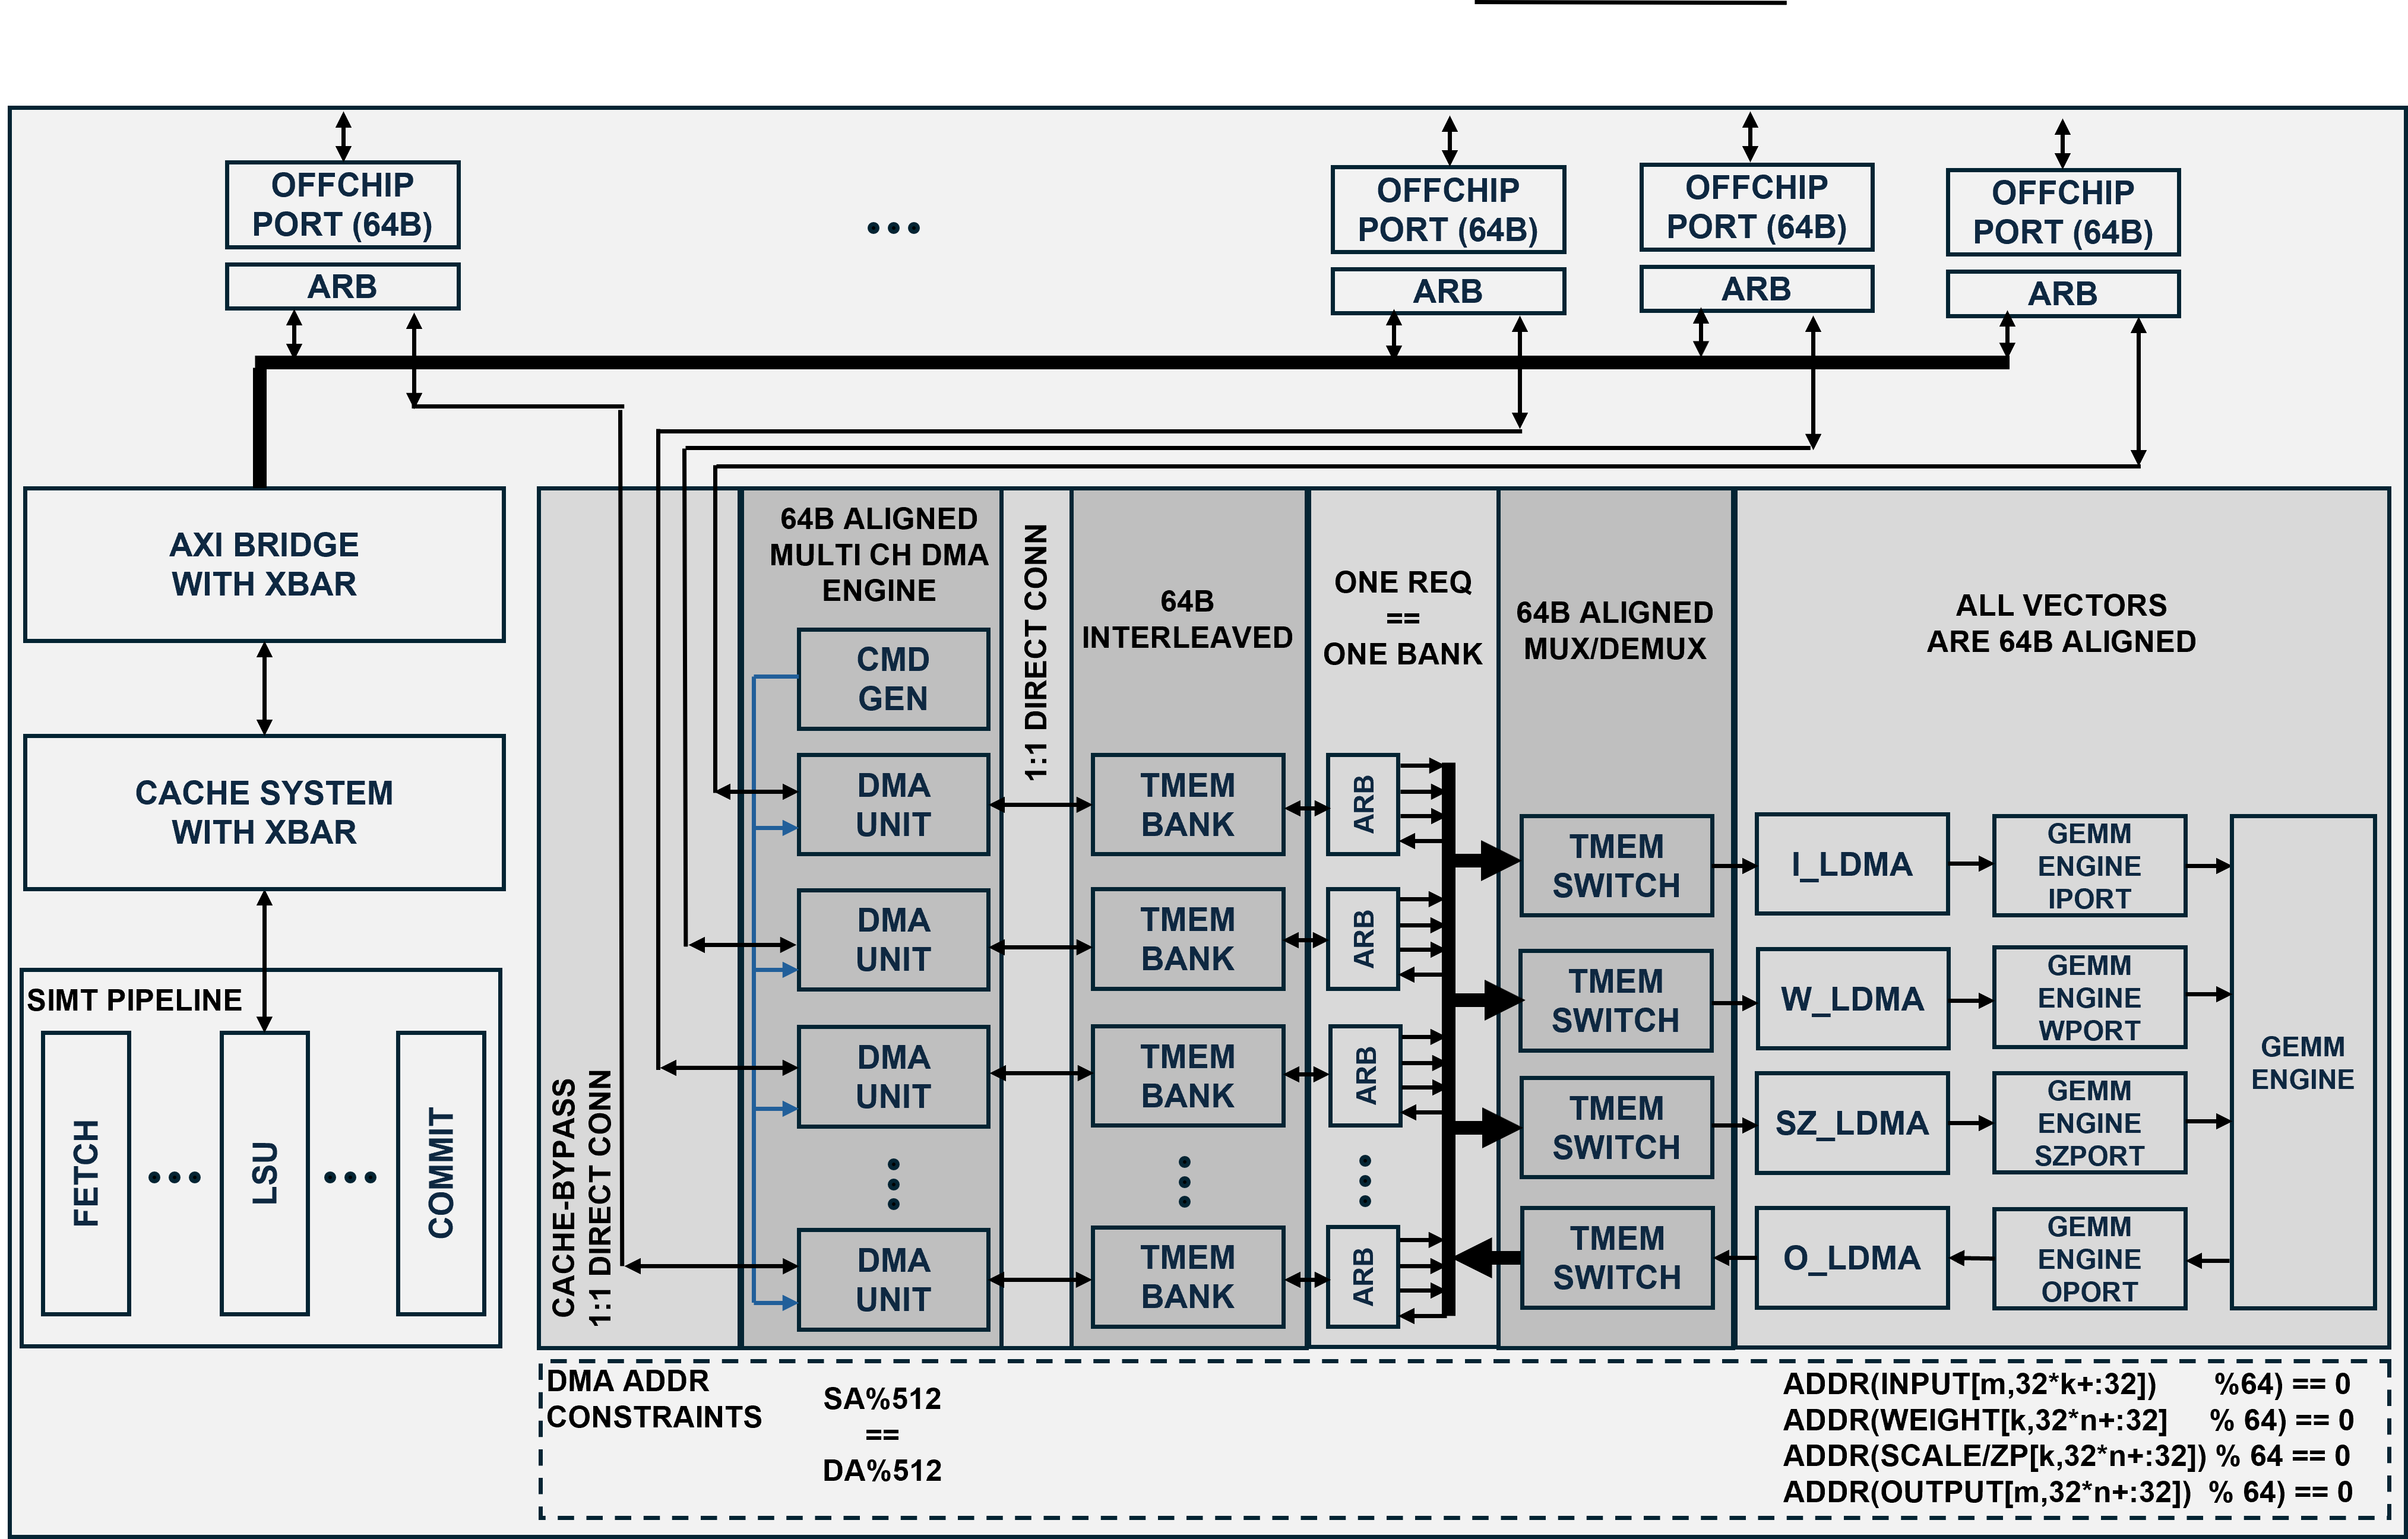
\includegraphics[width=0.92\linewidth]{figures/mem_sub_system.png}
%     \caption{Memory system for sustaining large \fpint{} arrays with direct tensor data movement.}
%     \label{fig:memory-system}
% \end{figure}
%\begin{figure*}[t]
%    \centering
%    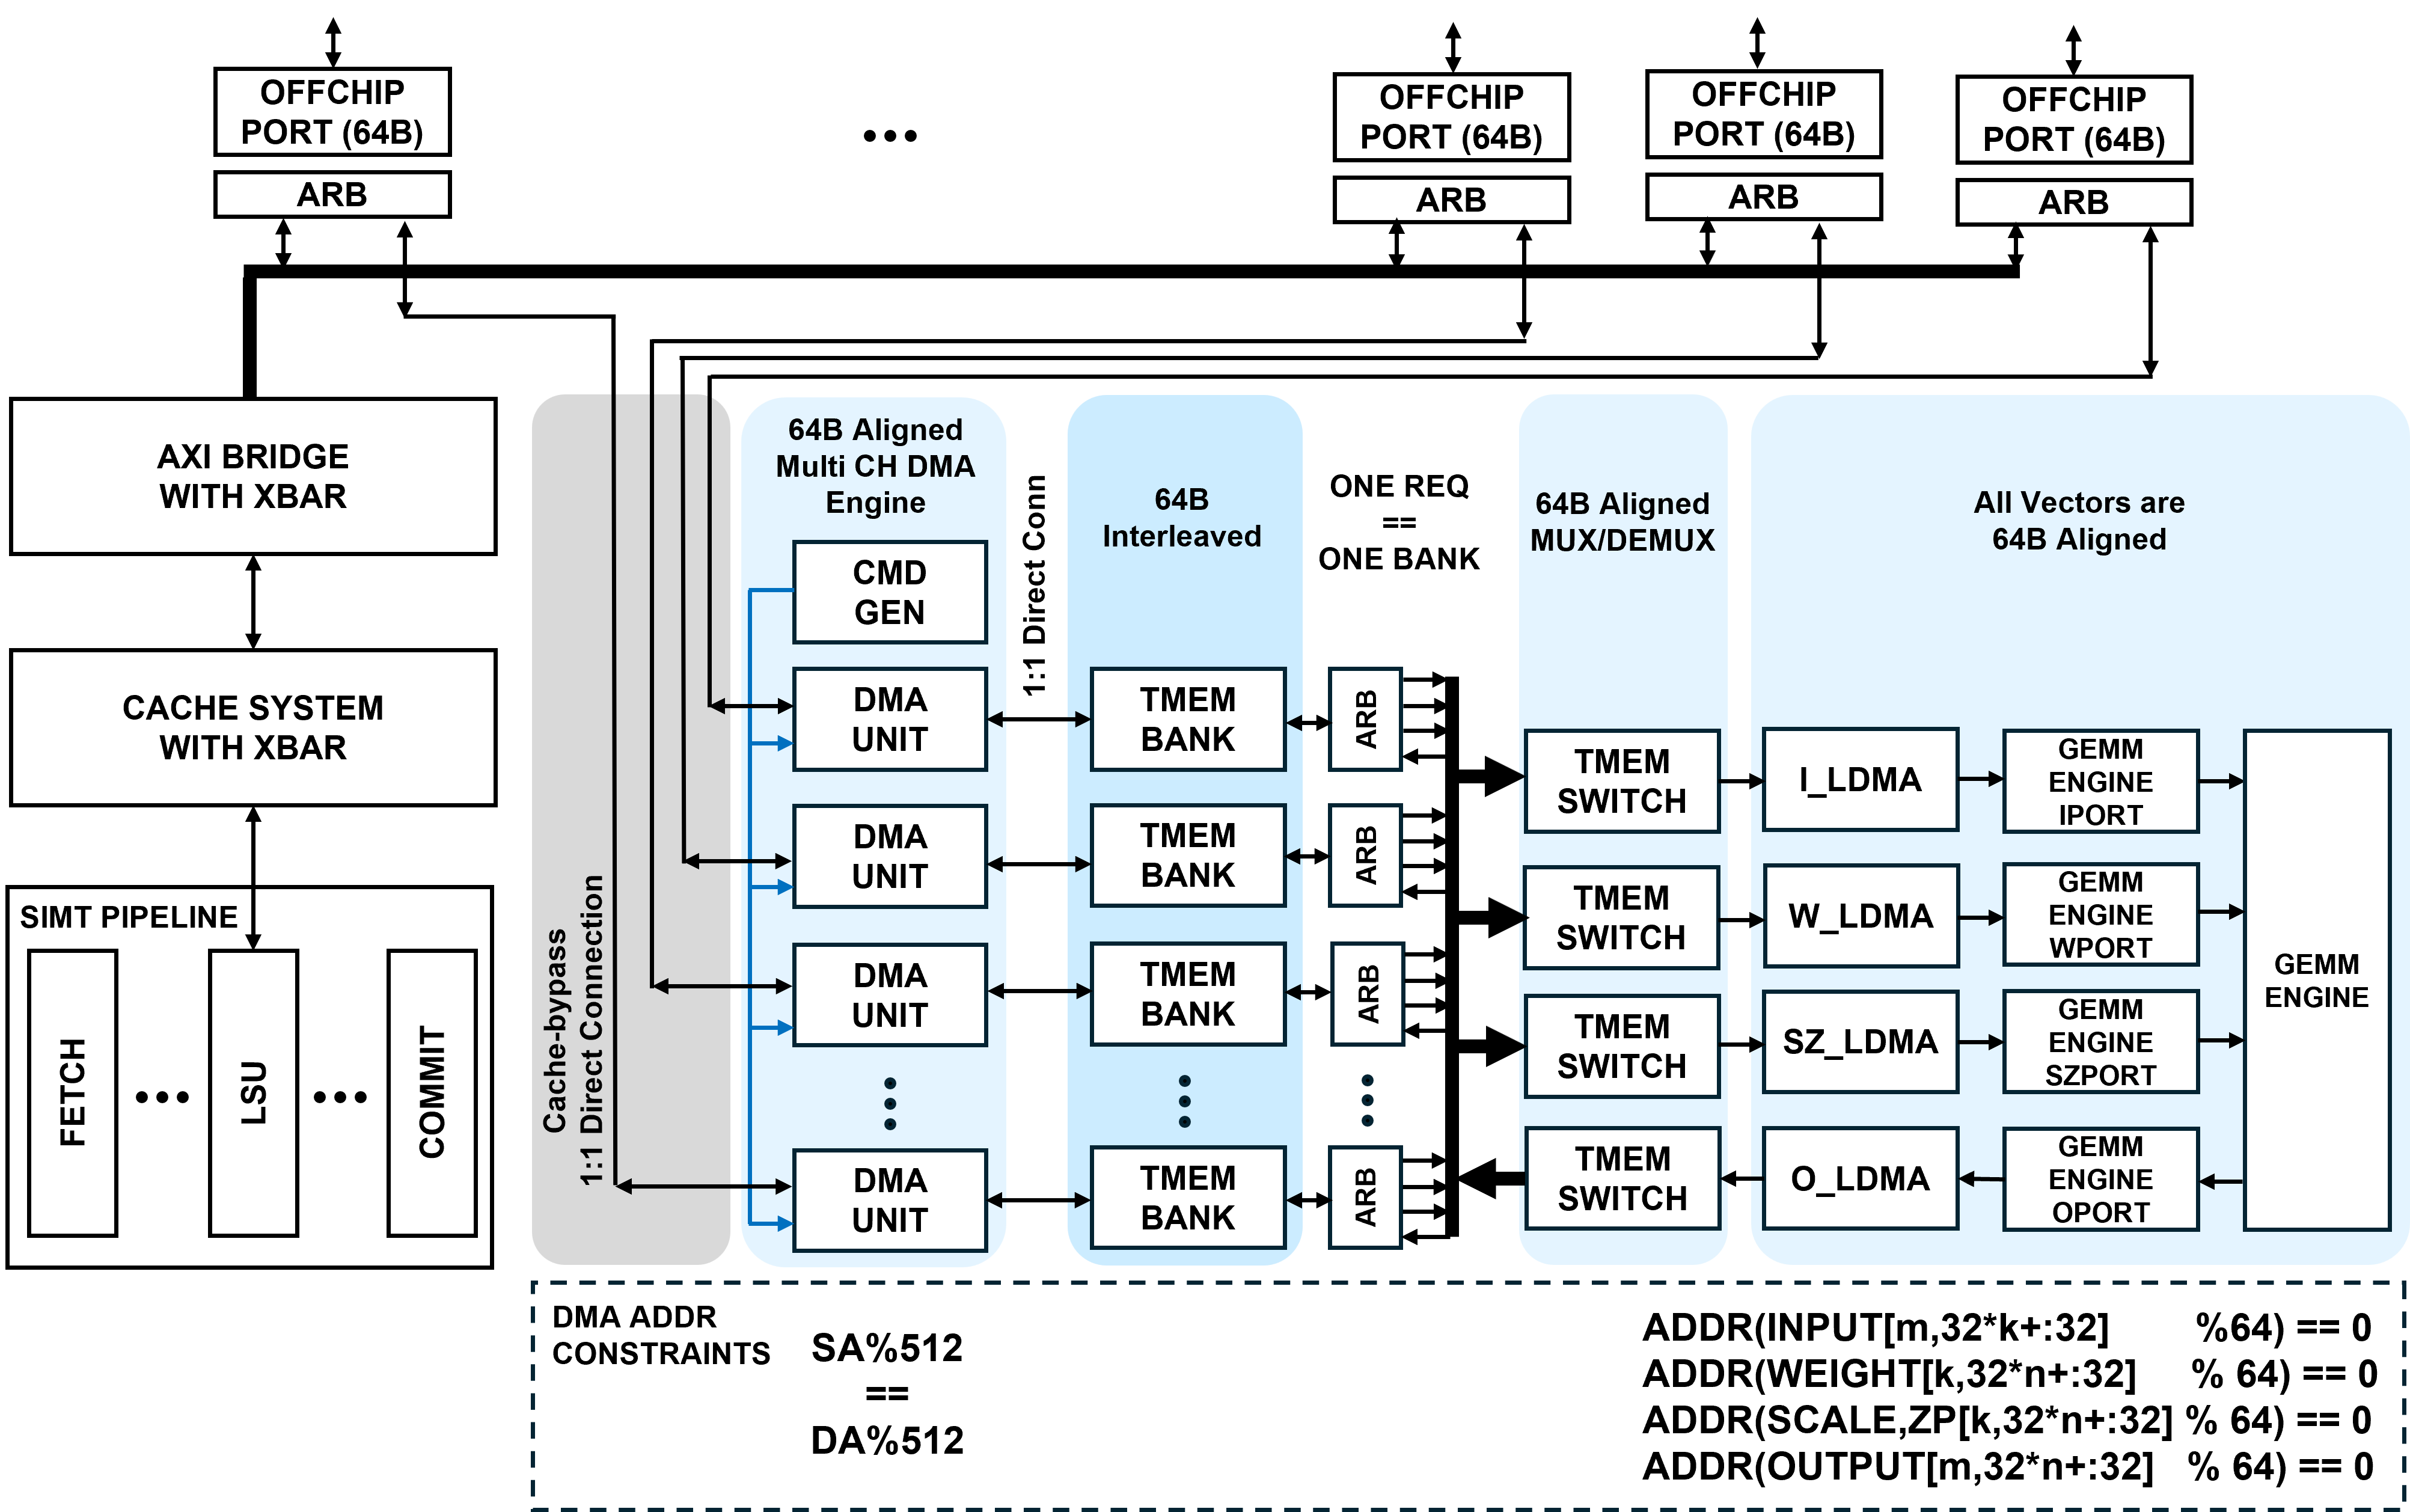
\includegraphics[width=0.96\textwidth]{figures/figs_fig9.png}
%    \caption{Memory system for sustaining large \fpint{} arrays with direct tensor data movement.}
%    \label{fig:memory-system}
%\end{figure*}

\begin{figure}[t]
    \centering
    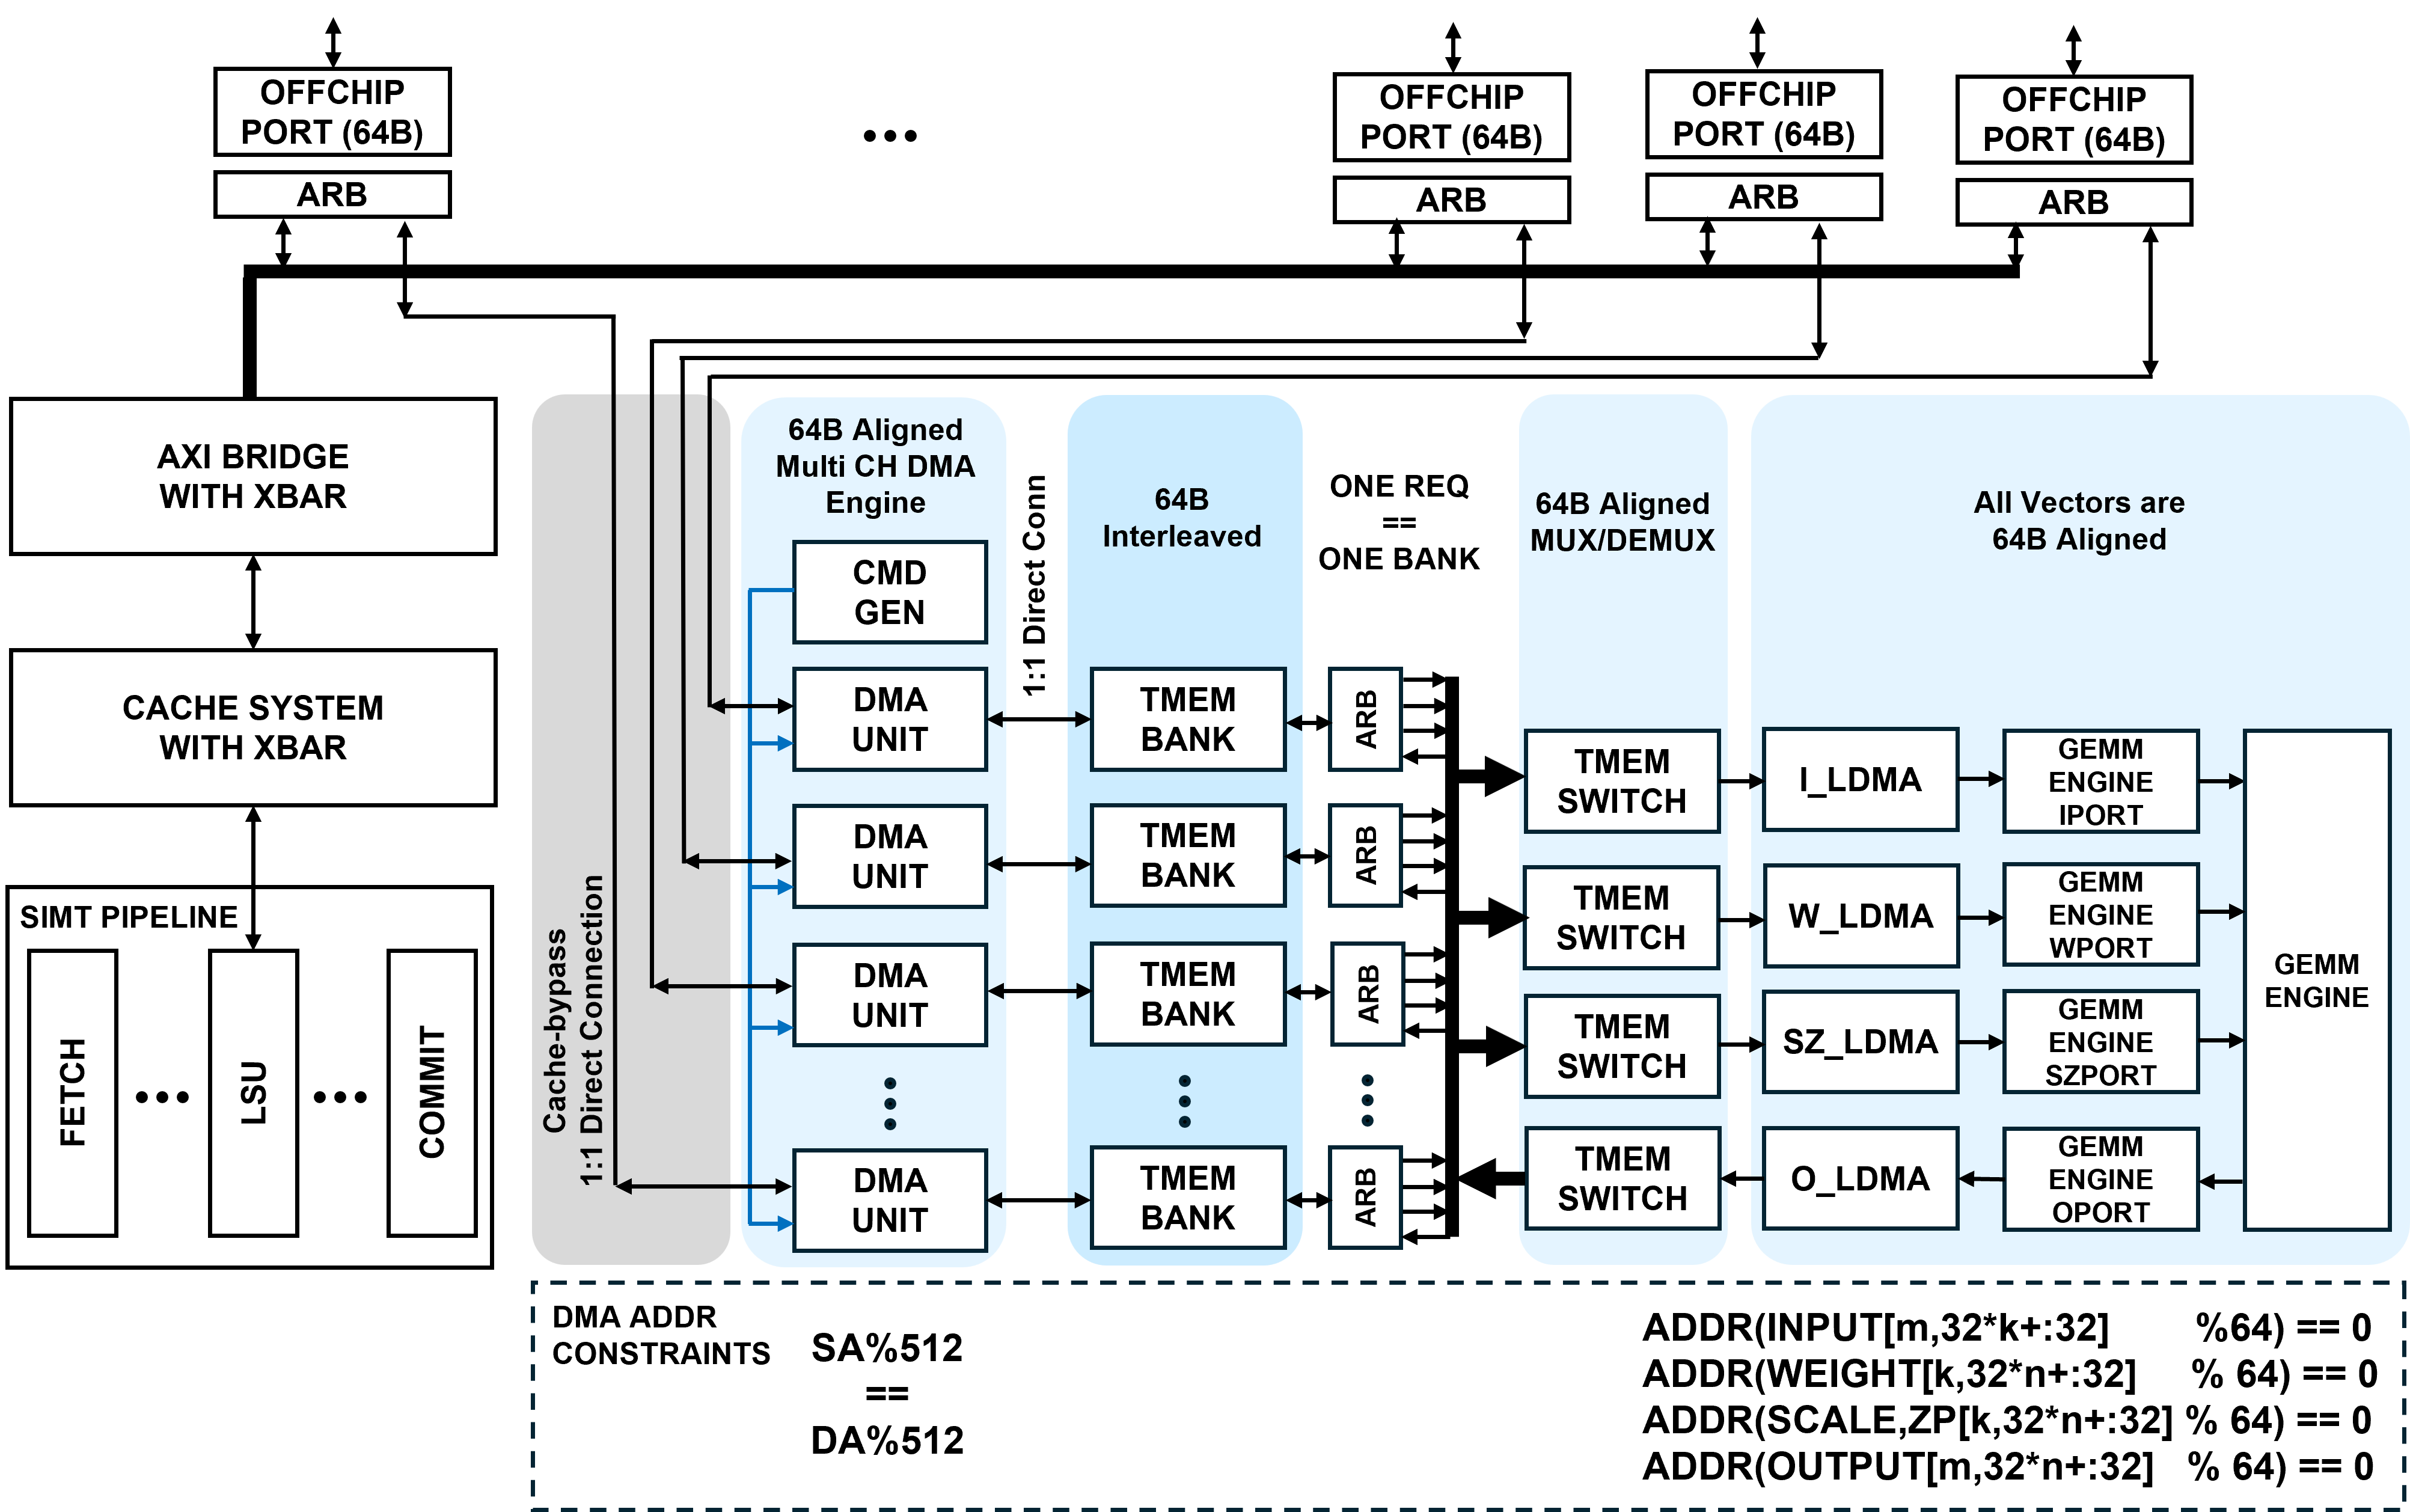
\includegraphics[width=0.92\linewidth]{figures/figs_fig9.png}
    \caption{Memory system for sustaining large \fpint{} arrays with direct tensor data movement.}
    \label{fig:memory-system}
\end{figure}

%\textbf{Cache-Bypassed Tensor DMA.}
\textbf{Tensor DMA and MXU DMA.}
Tensor traffic between HBM and TMEM banks also bypasses the cache hierarchy. Routing it through the cache would put it on paths shared with cache banks, local memory, and SIMT load/store, making crossbar and multi-bank arbitration costs the bottleneck again. \ours{} instead moves tensor data directly from HBM pseudo-channels to tensor memory banks, reducing cache pollution and port conflicts. Because this path is outside the coherent cache protocol, Section~\ref{sec:runtime-section} handles visibility through a producer fence, result tile completion polling, and mandatory cache management at kernel boundaries.
Separately, between the TMEM banks and the GEMM engine, four independent I/W/SZ/O DMA engines transfer input, weight, scale/zero-point, and output tensors in parallel.
Overall, descriptor-driven GEMM execution, partitioned tensor storage, interleaved-connected DMA, and cache bypass prevent \fpint{} array efficiency from being lost to operand supply.
\fi

\section{Constraint-Aware Layout and Runtime Support}
\label{sec:runtime-section}

% The low-cost tensor path in Section~\ref{sec:memory-system} exposes two address constraints to software. A T-DMA transfer must satisfy both the HBM--TMEM endpoint-mapping constraint in Eq.~\ref{eq:general_interleaved_constraint} and the $DW$-byte alignment constraint in Eq.~\ref{eq:aligned_dma_constraint}. Independently, every G-DMA port word must satisfy the 64\,B TMEM alignment constraint in Eq.~\ref{eq:tmem_gemm_vector_constraint}. \ours{} absorbs both in software through alignment-aware allocation, tile-major layouts, and fused layout transformation, keeping tensors in a form the simplified path can consume without a complex interconnect.
The tensor path in Section~\ref{sec:memory-system} trades interconnect cost for three software-visible address constraints: \eqref{eq:general_interleaved_constraint} and \eqref{eq:aligned_dma_constraint} on every T-DMA transfer, and \eqref{eq:tmem_gemm_vector_constraint} on every G-DMA port word. FINISH absorbs all three through alignment-aware allocation, tile-major layouts, and fused layout transformation.

\subsection{Power-of-Two Mapping and Aligned Allocation}
\ours{} restricts the HBM pseudo-channel count $N_{\mathrm{pc}}$ and the TMEM bank count $N_{\mathrm{tmem}}$ to powers of two so that the smaller count divides the larger one, simplifying the mapping constraint. Define the HBM--TMEM mapping period as
\begin{equation}
    N_{\min}^{HT}
    =
    \min
    \left(
        N_{\mathrm{pc}},
        N_{\mathrm{tmem}}
    \right),
    \qquad
    P_{HT}
    =
    DW \cdot N_{\min}^{HT}.
    \label{eq:hbm_tmem_mapping_period}
\end{equation}
For the $DW$-aligned addresses required by \eqref{eq:aligned_dma_constraint}, the general endpoint-mapping constraint reduces to
\begin{equation}
    A_{\mathrm{HBM}}
    \equiv
    A_{\mathrm{TMEM}}
    \pmod{P_{HT}}.
    \label{eq:interleaved_address_constraint}
\end{equation}
\ours{} extends the Vortex runtime so an allocation can constrain both size and base-address alignment, jointly selecting the HBM and TMEM bases of each tile to satisfy \eqref{eq:interleaved_address_constraint}. Adding the same tile-local offset to both bases preserves the congruence, so all corresponding $DW$-byte words stay connected. 
%With tile sizes that are multiples of $P_{HT}$ and every G-DMA port word placed at a multiple of 64\,B, successive T-DMA tiles preserve the mapping and each I/W/SZ/O word begins at a legal TMEM address.
To show how the tiled layout preserves this congruence, we distinguish two tile levels: an outer L1 tile transferred by the T-DMA and an MXU-sized L2 tile within it.
Since $V_g=DW$ divides $P_{HT}=DW\cdot N_{\min}^{HT}$, $P_{HT}$-aligned L1 bases and $P_{HT}$-multiple L1 footprints preserve the HBM-TMEM mapping, while $V_g$-multiple L2 footprints align all G-DMA words.
In Fig.~\ref{fig:tile-major-b}, a $128\times128$ INT4 L1 weight tile occupies 8\,KiB, and each contiguous $32\times32$ L2 tile occupies 512\,B; both are naturally aligned for $P_{HT}=512\,\mathrm{B}$ and $V_W=64\,\mathrm{B}$.

\subsection{Conflict-Free Tile-Major Layout}

\begin{figure}[t]
   \centering
   \begin{subfigure}[t]{0.45\linewidth}
       \centering
       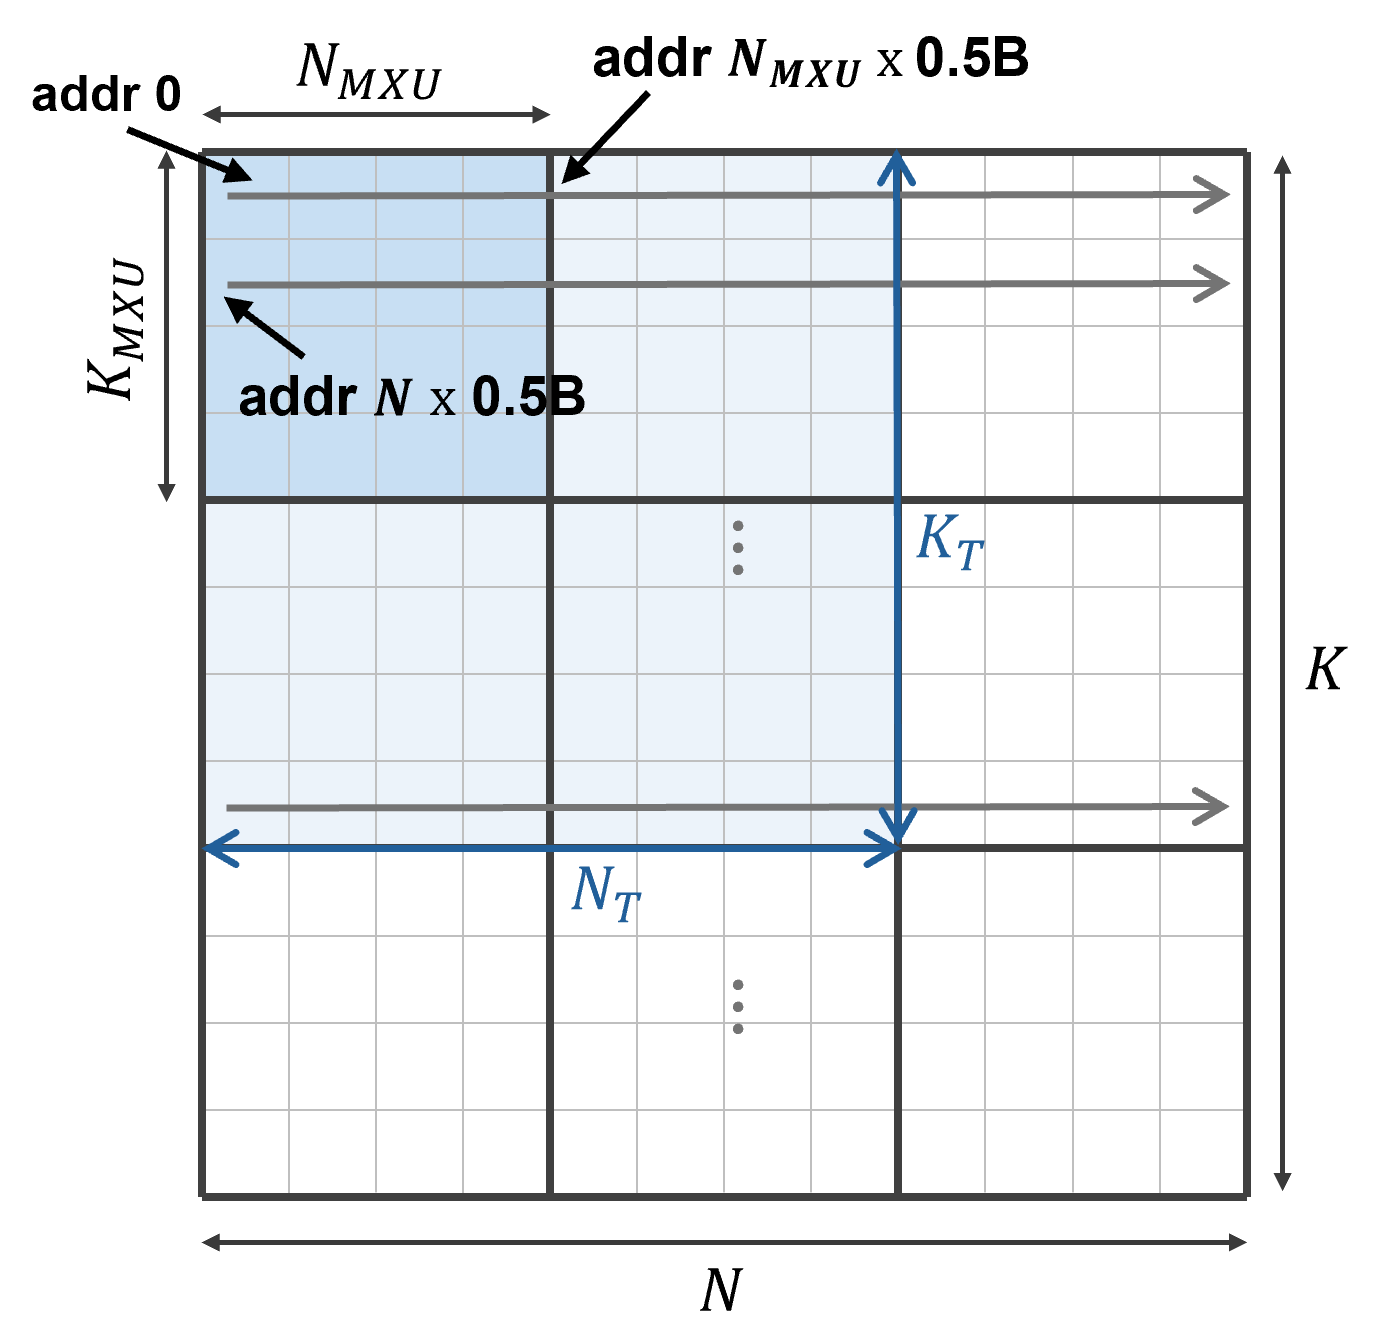
\includegraphics[width=\linewidth]{figures/tile-major-a.png}
       \caption{Row-major tensor layout.}
       \label{fig:tile-major-a}
   \end{subfigure}
   \hfill
   \begin{subfigure}[t]{0.48\linewidth}
       \centering
       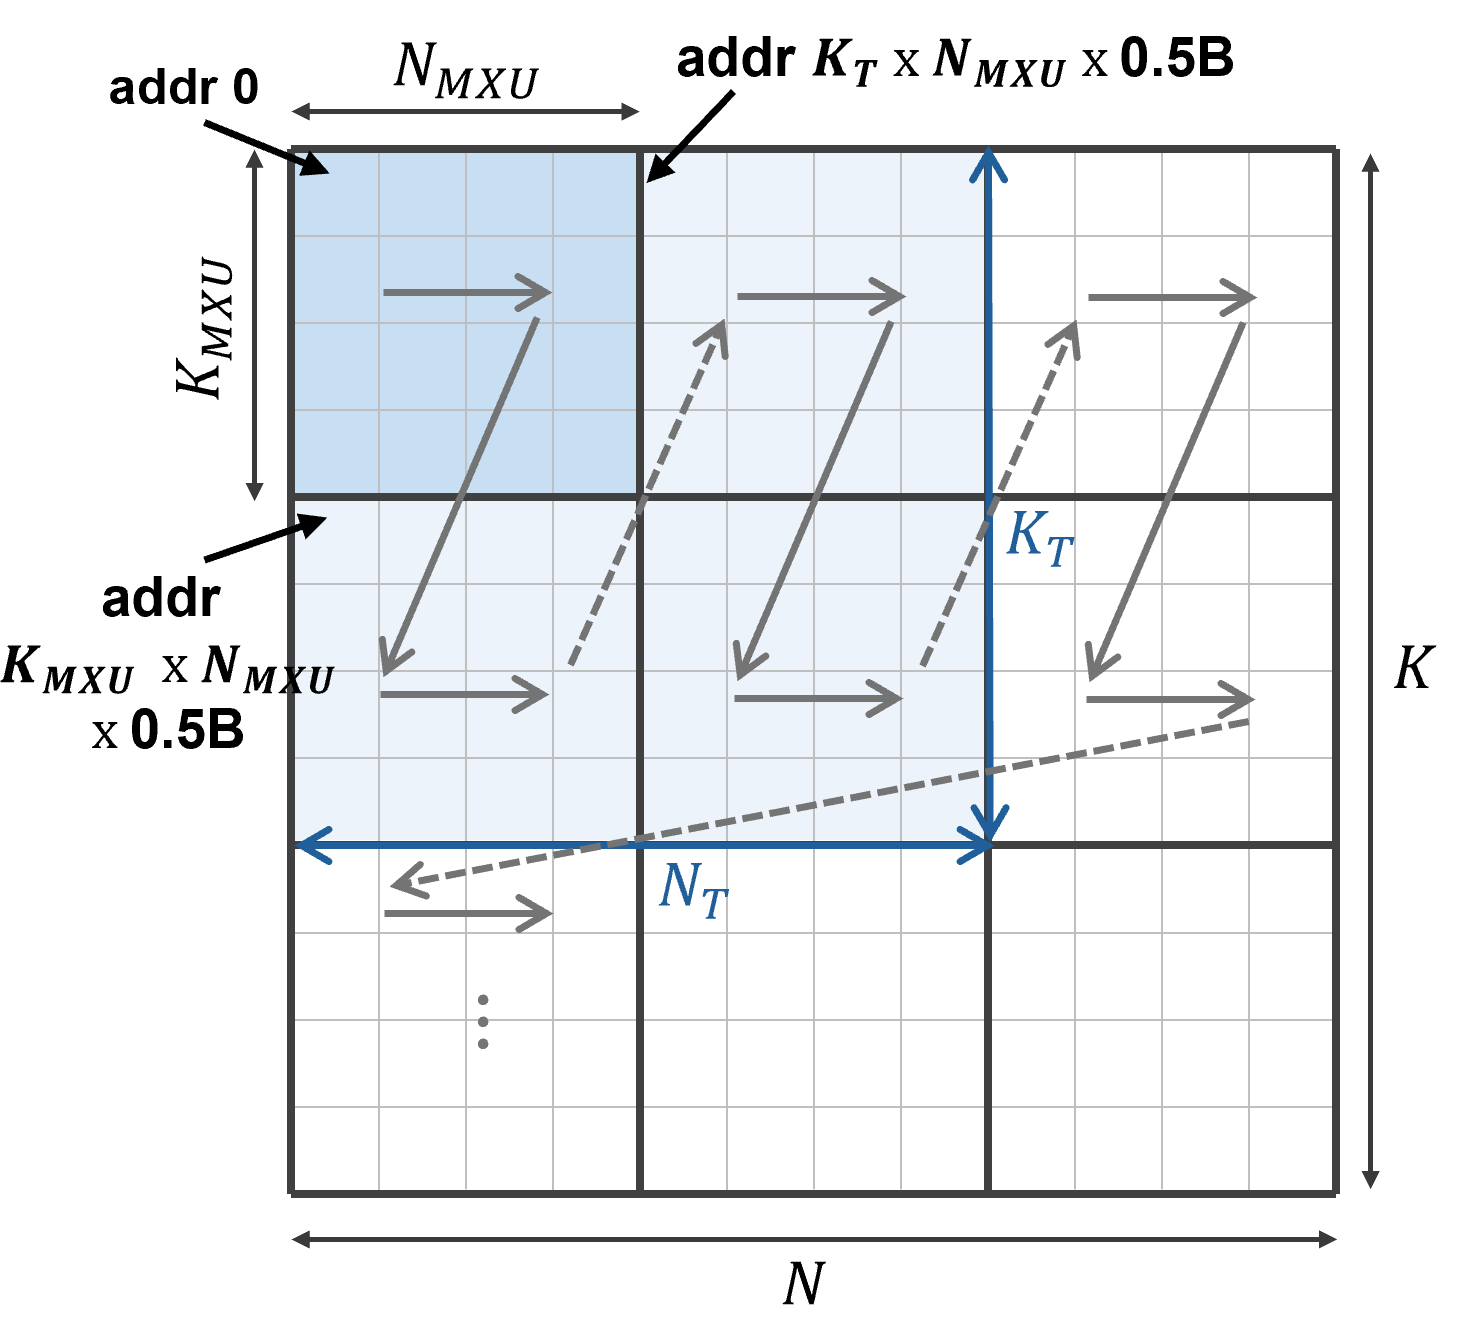
\includegraphics[width=\linewidth]{figures/tile-major-b.png}
       \caption{Tile-major tensor layout.}
       \label{fig:tile-major-b}
   \end{subfigure}
   \caption{Layout comparison for a representative weight tile. A row-major tile spans noncontiguous row segments, whereas tile-major storage makes the entire tile contiguous.}
   \label{fig:tile-major-layout}
\end{figure}

% ---------------------------------------------------------------------
% A padded row-major layout can satisfy both the address-congruence and alignment constraints discussed above. However, the row-major layout experiences inefficiency in the bank-access sequence during a high-bandwidth tile transfer.
% As shown in Fig.~\ref{fig:tile-major-a}, an $M_T \times K_T$ row-major tile consists of $M_T$ noncontiguous row segments. Within a segment, consecutive $DW$-byte words advance through consecutive banks. At a segment boundary, however, the address advances by the full padded row stride rather than by a tile-local contiguous offset. The next bank is therefore determined by the tensor shape and row stride, and multiple row segments issued in parallel may map to the same bank. Shape- and stride-dependent padding or bank-aware scheduling can avoid particular conflicts, but does not provide one general conflict-free mapping across supported tensor shapes.

% In contrast, in the tile-major layout in Figure~\ref{fig:tile-major-b}, all words of a tile form a contiguous sequence. Under the low-order interleaving used by \ours{}, consecutive aligned words rotate across consecutive banks. A T-DMA tile transfer can therefore use one word from each bank per interleaving round without conflicts, up to the aggregate bank bandwidth. This predictable bank sequence, rather than alignment alone, is the primary reason that \ours{} uses tile-major storage.

% \ours{} uses outer tile dimensions $M_T$, $K_T$, and $N_T$ for data transferred by the T-DMA and inner tile dimensions $M_{\mathrm{MXU}}$, $K_{\mathrm{MXU}}$, and $N_{\mathrm{MXU}}$ for data consumed through the G-DMA. Besides guaranteeing the address properties above, contiguous storage lets the runtime describe a tile as one aligned transfer rather than as separate requests for its row segments, satisfying the requirement for aligned-only T-DMA interface.
% ---------------------------------------------------------------------
% +++++++++++++++++++++++++++++++++++++++++++++++++++++++++++++++++++++
A padded row-major layout can satisfy the address-congruence and alignment constraints above, but it remains inefficient in its bank-access sequence during a high-bandwidth transfer. 
As shown in Fig.~\ref{fig:tile-major-a}, a $K_T \times N_T$ row-major tile spans $K_T$ noncontiguous row segments: words advance through consecutive banks within a segment, but at each segment boundary the address jumps by the full padded row stride, so the next bank depends on tensor shape and stride and parallel segments may collide on the same bank.
% Shape-dependent padding or bank-aware scheduling avoids particular conflicts but not all of them across supported shapes.
Shape-dependent padding or bank-aware scheduling can avoid particular conflicts, but does not guarantee conflict-free transfers across all supported shapes.
Moreover, the noncontiguous row segments break long DMA bursts at row boundaries, increasing the number of burst transactions per tile.

In the tile-major layout of Fig.~\ref{fig:tile-major-b}, all words of a tile are contiguous, so under low-order interleaving they rotate across consecutive banks and a T-DMA transfer uses one word per bank each round without conflict, up to the aggregate bank bandwidth. This predictable bank sequence, rather than alignment alone, is why \ours{} adopts tile-major storage, and it also lets the runtime describe each tile as one aligned transfer instead of per-row-segment requests.
% +++++++++++++++++++++++++++++++++++++++++++++++++++++++++++++++++++++

\subsection{Fused Layout Transformation}
\begin{figure}[t]
    \centering
    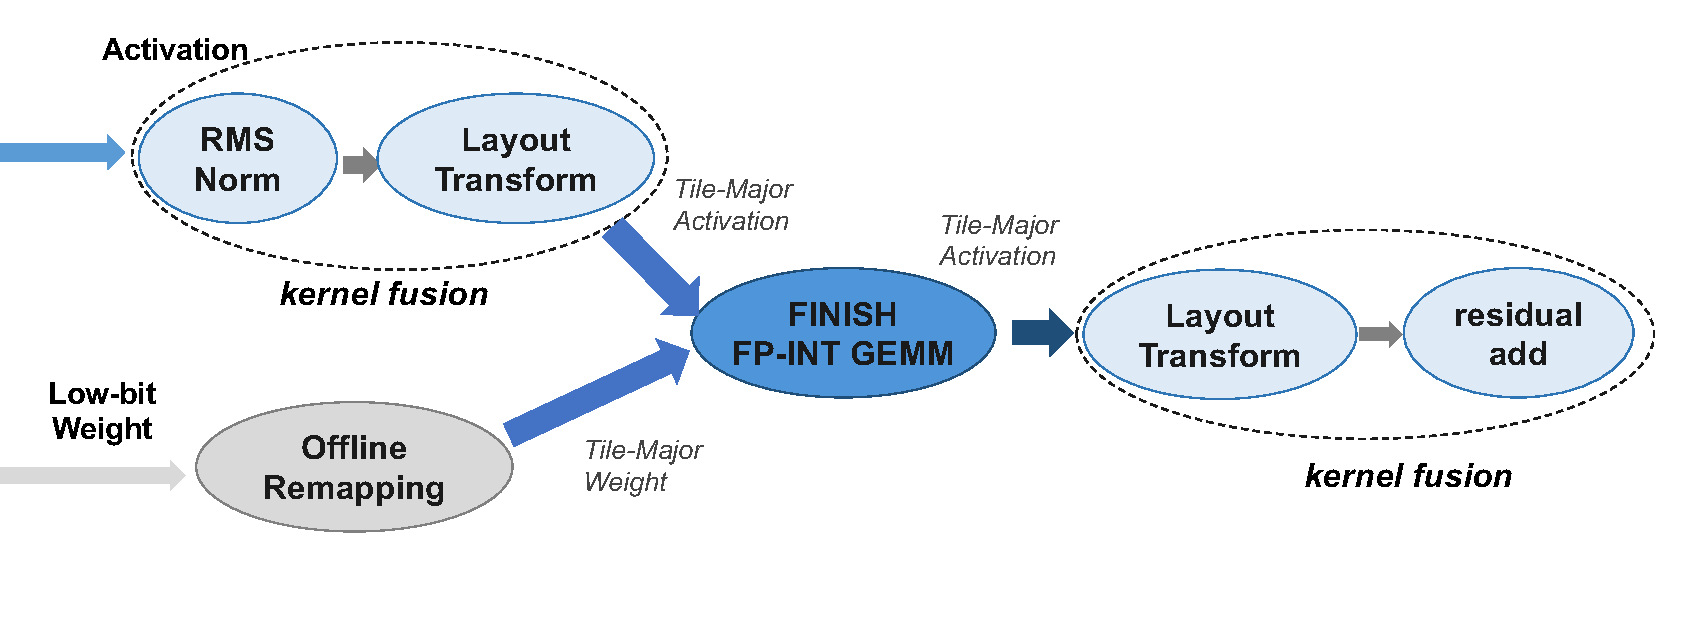
\includegraphics[width=0.92\linewidth]{figures/fig9_layout_fusion.pdf}
    \caption{Fused layout transformation for the cache-bypassed tensor path, showing representative sites for offline and fused transformations.}
    \label{fig:fuse_layout_transform}
\end{figure}

Converting every tensor with a separate layout-transformation kernel would add a memory pass that offsets the benefit of the tensor path\cite{ladder,tvm,shi2023welder,zhu2022roller,tillet2019triton}. \ours{} therefore remaps static weights to tile-major form offline and, for dynamically produced tensors, fuses the transformation into the vector kernels adjacent to a GEMM, such as RMSNorm, RoPE, softmax, and residual addition (Fig.~\ref{fig:fuse_layout_transform}). A preceding kernel writes its output directly in aligned tile-major form and a following kernel consumes the tile-major GEMM output as part of its normal computation, so tensors reach the T-DMA and G-DMA without a standalone conversion pass at the GEMM boundary.

\begin{comment}
\section{Layout transformation and runtime optimization}
\label{sec:runtime-section}

\begin{figure}[t]
    \centering
    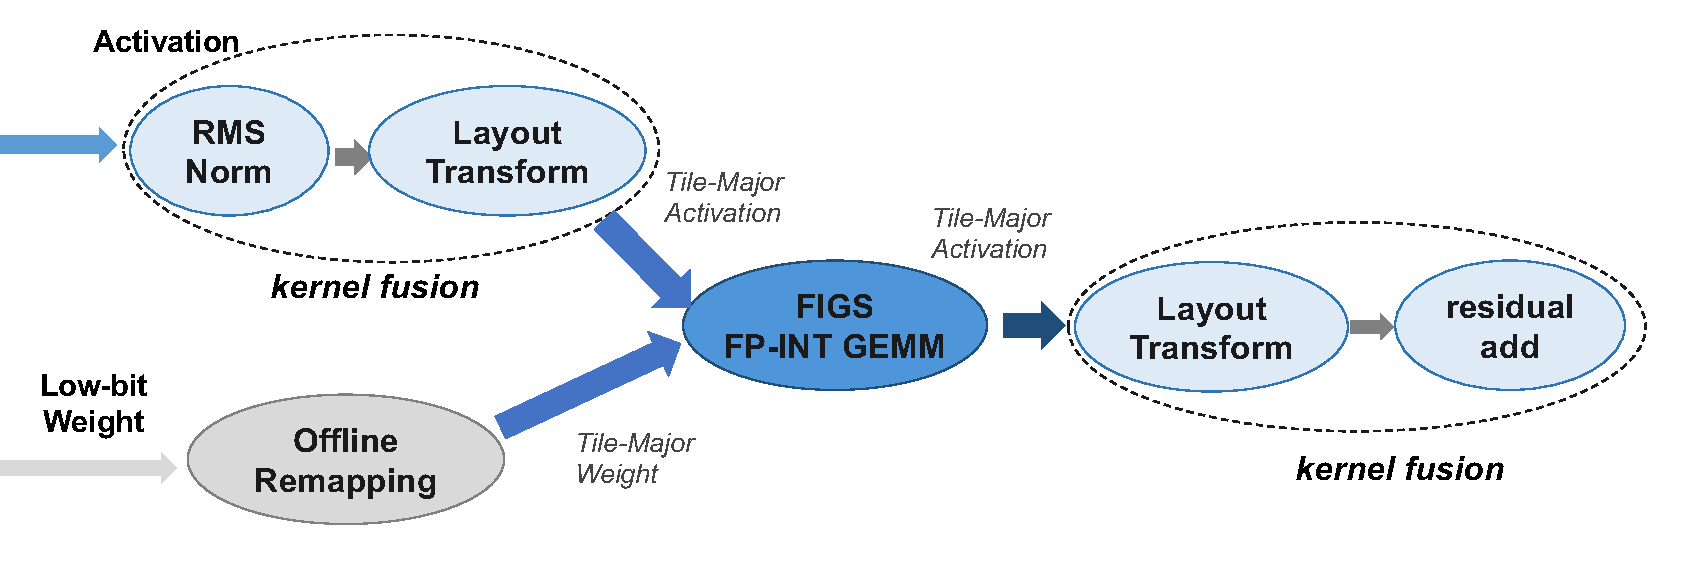
\includegraphics[width=0.92\linewidth]{figures/layout_fusion.pdf}
    \caption{Fused layout transformation for feeding cache-bypassed tensor DMA. The figure is simplified and shows representative fusion sites only.}
    \label{fig:fuse_layout_transform}
\end{figure}

The memory system of Section~\ref{sec:memory-system} simplifies hardware at the cost of three software-visible constraints: address alignment, bank mapping, and non-coherent DMA. \ours{} satisfies them by exploiting GEMM's regular tile-access pattern with tile-major layout, fused layout transformation, and alignment-aware allocation. Instead of relying on a complex interconnect, the software keeps both tensor layout and placement in a hardware-friendly form.
 
\textbf{Tile-major Layout and Aligned Allocation.}
\ours{} meets the constraints of Section~\ref{sec:memory-system} by changing the tensor layout to a tile-major form, choosing tile sizes appropriately, and jointly controlling the base address at which the tile is allocated in memory.

\begin{figure}[t]
   \centering

   \begin{subfigure}[t]{0.45\linewidth}
       \centering
       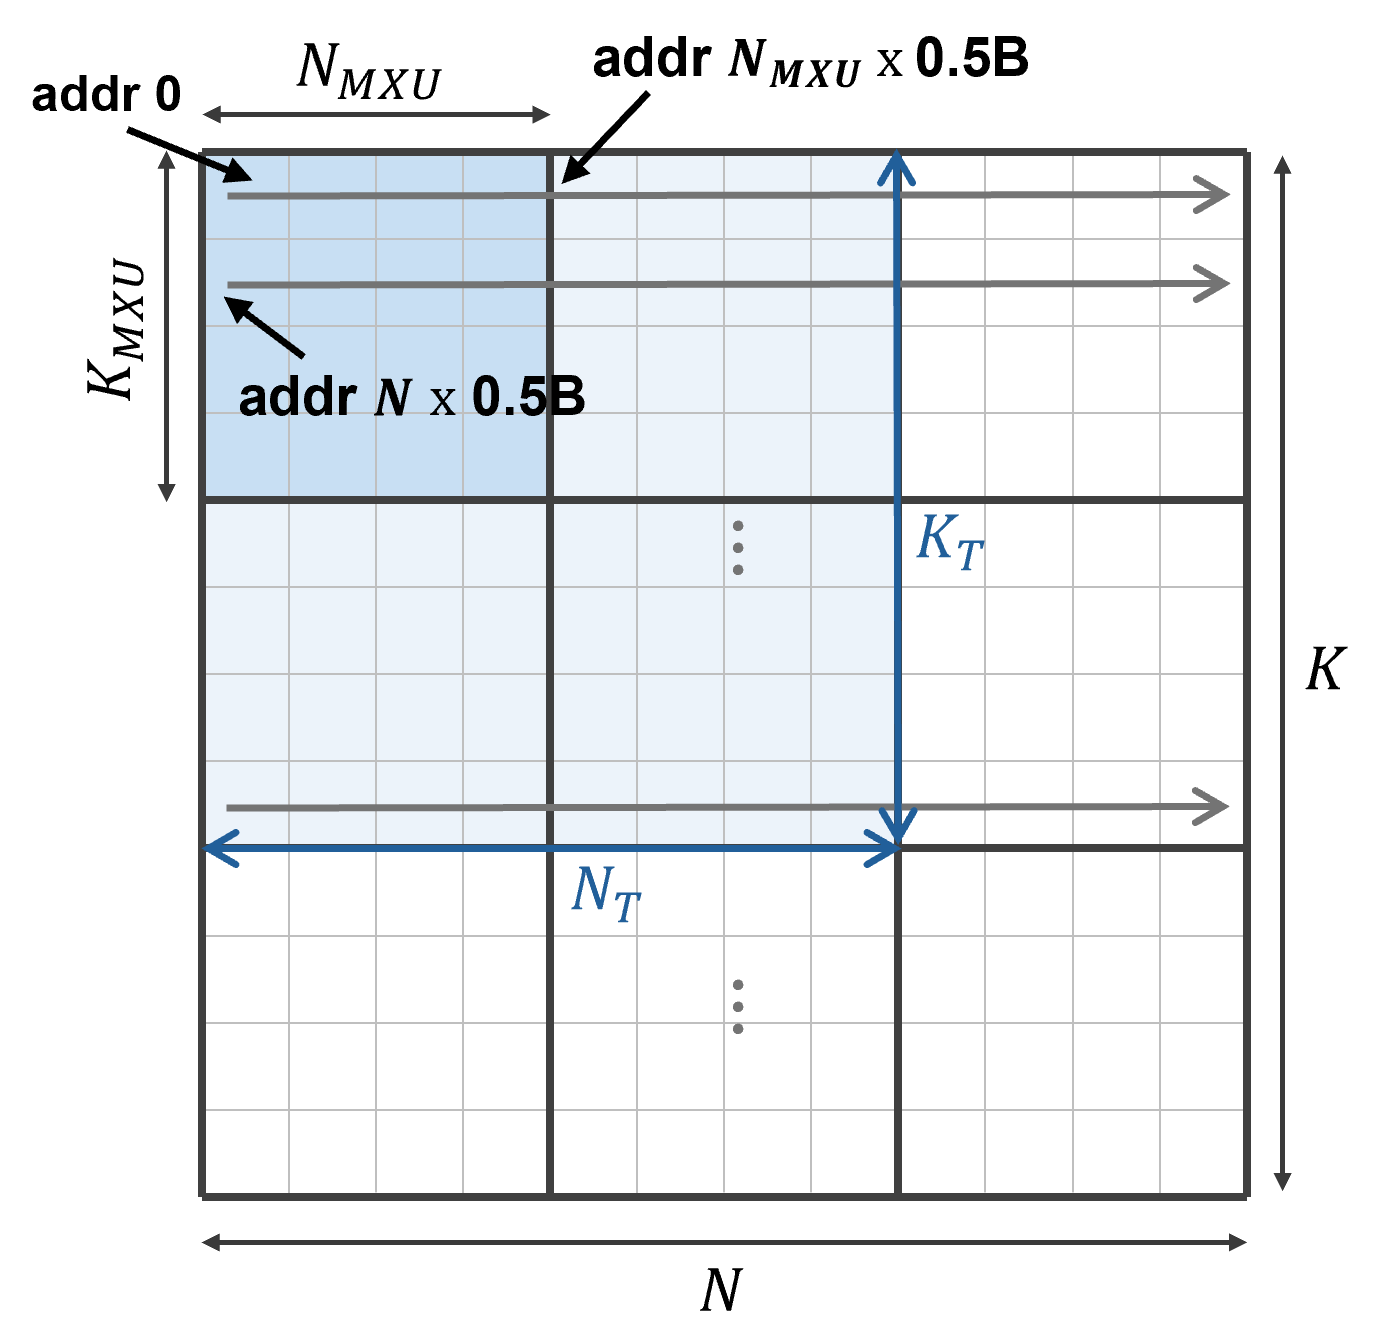
\includegraphics[width=\linewidth]{figures/tile-major-a.png}
       \caption{Row-major weight layout.}
       \label{fig:tile-major-a}
   \end{subfigure}
   \hfill
   \begin{subfigure}[t]{0.48\linewidth}
       \centering
       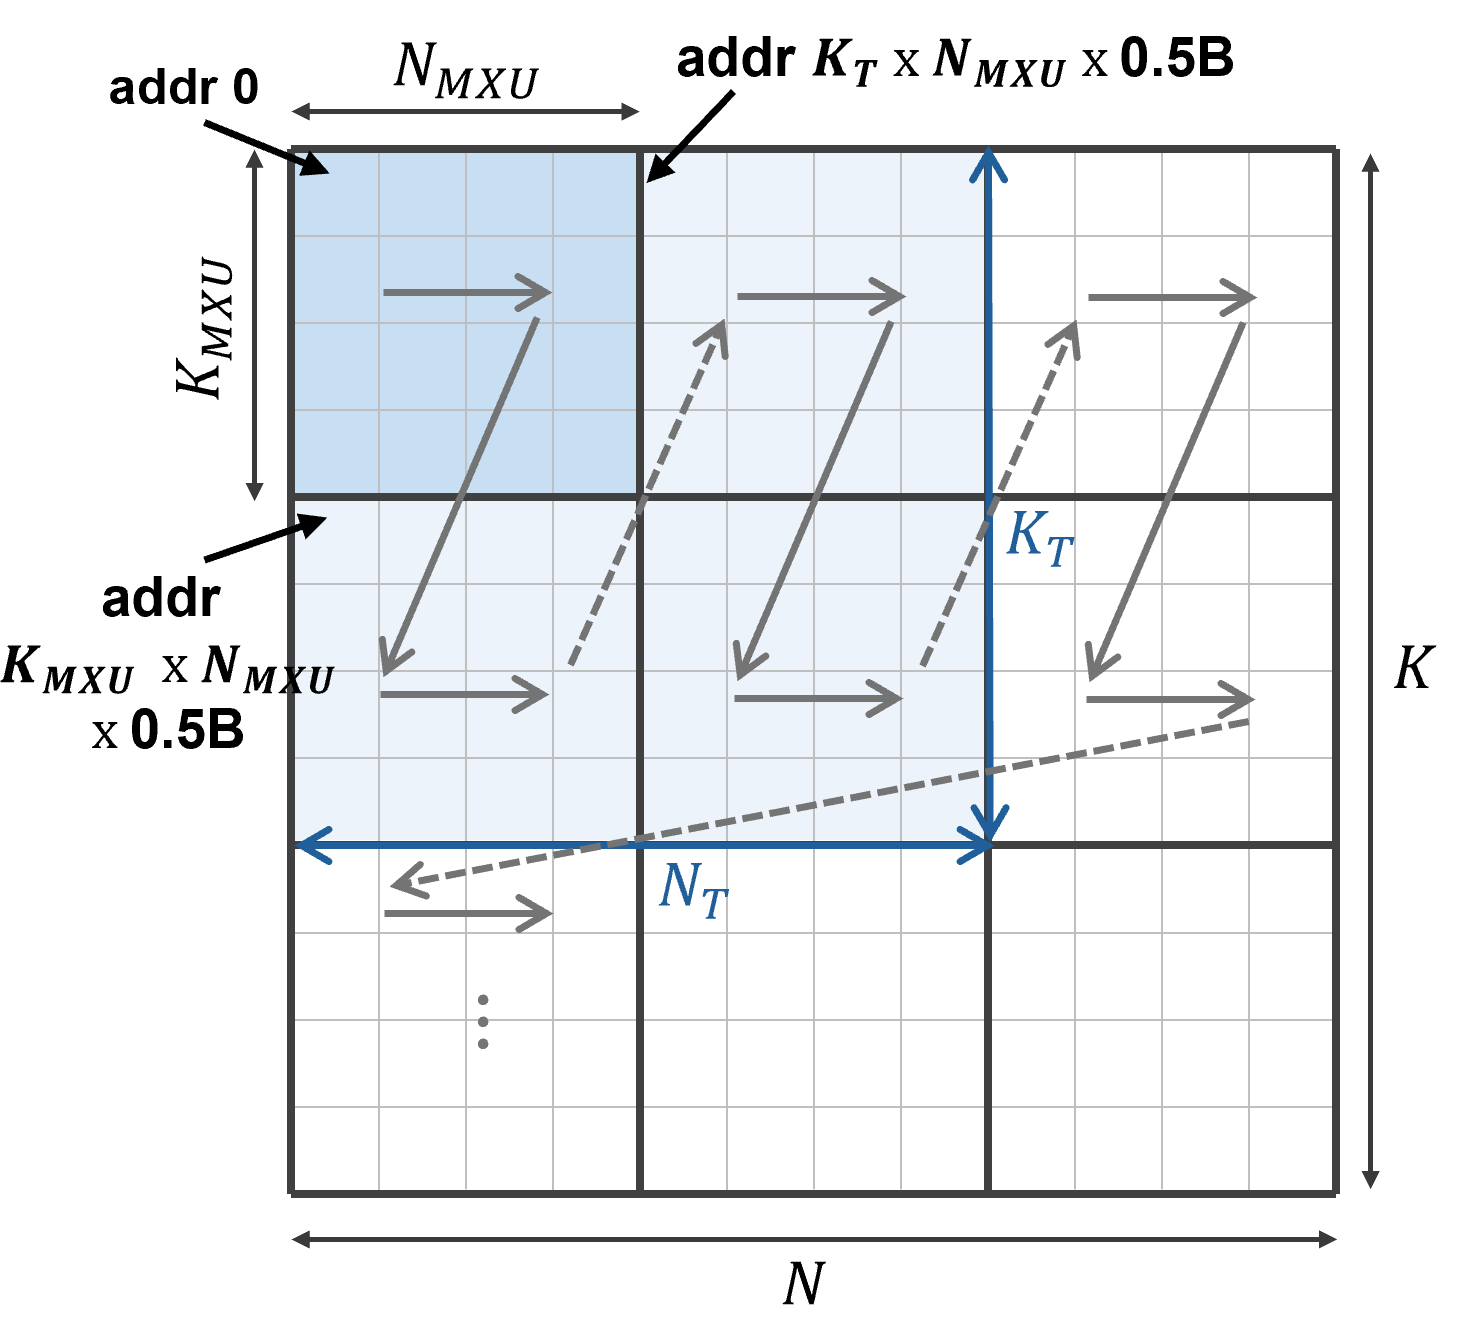
\includegraphics[width=\linewidth]{figures/tile-major-b.png}
       \caption{Tile-major weight layout.}
       \label{fig:tile-major-b}
   \end{subfigure}

   \caption{In the row-major layout, a tile spans multiple noncontiguous row segments, whereas the tile-major input and weight layouts store each tile in a contiguous memory region.}
   \label{fig:tile-major-layout}
\end{figure}

% \begin{figure}[t]
%    \centering
%    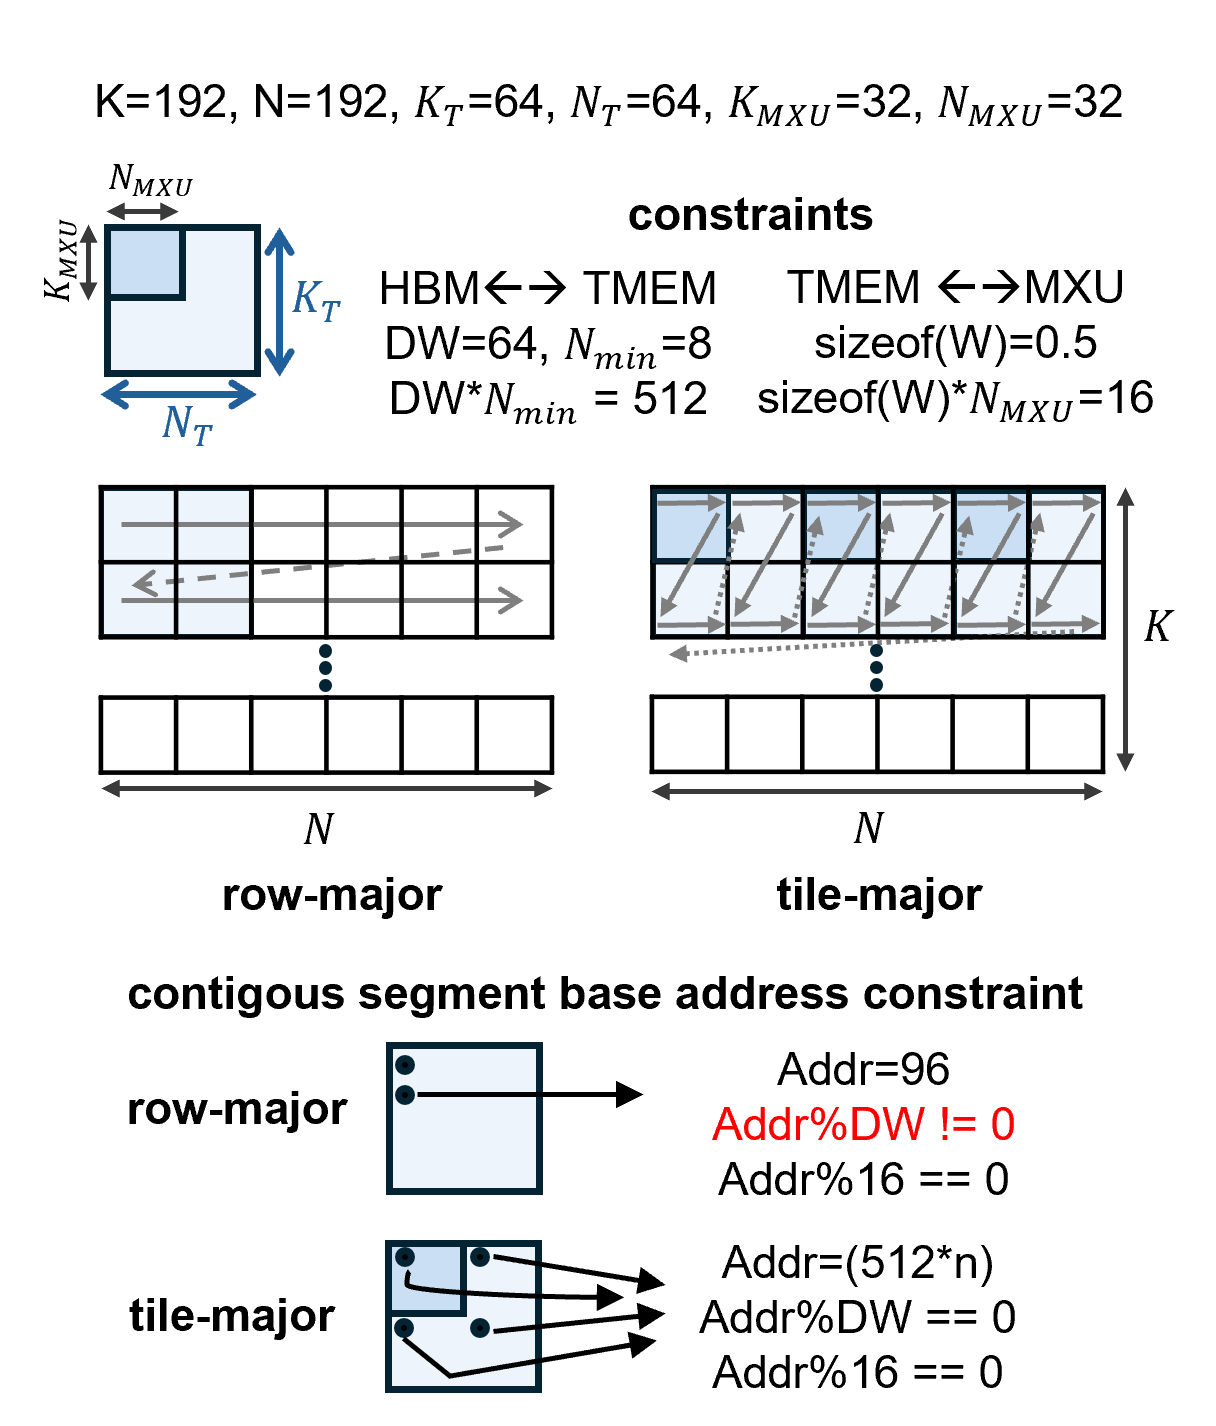
\includegraphics[width=0.9\linewidth]{figures/layout.png}
%    \caption{In the row-major layout, a tile spans multiple noncontiguous row segments, whereas the tile-major input and weight layouts store each tile in a contiguous memory region.}
%    \label{fig:tile-major-layout}
% \end{figure}

\ours{} launches a SIMT kernel that transforms GEMM input and output tensors into a format organized by tiles. The layout uses tile dimensions $M_T$, $K_T$, and $N_T$ for data transferred from HBM to tensor memory. It uses a second tile shape, defined by $K_{\mathrm{MXU}}$ and $N_{\mathrm{MXU}}$, for operand tiles consumed by the GEMM engine from tensor memory. Each tile size is a multiple of the %alignment granularity
moduli specified in Section~\ref{sec:memory-system}, and elements within a tile are contiguous, so the address constraints are met by construction.

Figure~\ref{fig:tile-major-layout} illustrates how the tile-major layout enables an efficient high-bandwidth DMA implementation. In the row-major layout shown in Fig.~\ref{fig:tile-major-a}, an $M_T \times K_T$ tile is distributed across $M_T$ noncontiguous row segments. Because the base address of each segment is determined by the full row stride, these segments are not necessarily aligned to the wide DMA datapath. The DMA must therefore support misaligned accesses. Although realignment is relatively inexpensive for a narrow datapath, its hardware cost grows substantially as the DMA width increases: a single-cycle implementation requires a wide barrel shifter, whereas a multi-cycle implementation increases transfer latency. Hiding this additional latency requires more outstanding-request buffer entries, further increasing the area and complexity of the DMA engine.
Moreover, because the row segments are noncontiguous in a row-major layout, an interleaved memory address mapping may map multiple segments to the same bank, increasing the likelihood of bank conflicts.
In contrast, the tile-major layout in Fig.~\ref{fig:tile-major-b} stores all $M_T \times K_T$ elements of a tile contiguously and aligns each tile to the DMA transfer width. The tile can therefore be transferred using an aligned-only DMA without a wide realignment datapath or additional buffering for multi-cycle misaligned accesses.
In contrast, the tile-major layout stores addresses within each tile contiguously, guaranteeing conflict-free bank accesses unless the requested bandwidth exceeds the aggregate bank bandwidth.
As shown in Fig.~\ref{fig:tile-major-c}, FINISH applies the same organization to the weight tensor. Moreover, because TMEM is a tightly coupled memory with a short request-to-response latency, unlike GPU local memory whose access latency is approximately ten cycles, the TMEM--MXU DMA requires fewer outstanding requests to sustain bandwidth. Together, aligned tile-major accesses and low-latency TMEM enable a simpler and more efficient high-bandwidth DMA implementation.

%Figure~\ref{fig:tile-major-layout} illustrates how this organization reduces DMA command overhead. In the row-major layout shown in Fig.~\ref{fig:tile-major-a}, an $M_T \times K_T$ tile is divided across $M_T$ noncontiguous row segments. For illustration, assume that the tile begins at address 0, each element occupies 2 bytes, and each row contains $K$ elements. The DMA transfers the first $K_T$ elements by issuing a $K_T \times 2$ bytes request at address 0. It then transfers the second row segment by issuing another $K_T \times 2$-byte request at address $K \times 2$. Repeating this process for all rows requires a total of $M_T$ DMA commands. In contrast, the tile-major layout in Fig.~\ref{fig:tile-major-b} stores all $M_T \times K_T$ elements of the tile contiguously. The DMA can therefore fetch the entire tile from address 0 using a single command that transfers $M_T \times K_T \times 2$ bytes. As shown in Fig.~\ref{fig:tile-major-c}, \ours{} applies the same organization to the weight tensor.

\ours{} extends the Vortex runtime so memory allocation can constrain both requested size and base-address alignment. The runtime applies this constraint jointly to HBM and tensor-memory allocations so Eq.~\ref{eq:interleaved_address_constraint} holds. Kernels pass aligned tensor objects and tile descriptors to the DMA rather than arbitrary pointers, allowing the DMA to issue aligned bursts without a wide barrel shifter or general crossbar.

%Tile-major layout and alignment also improve DMA efficiency. A DMA request is most efficient when it moves a large contiguous segment; repeated small row-major or column-major requests create bubbles on long-latency paths. With tile-major layout, the requested tile is contiguous and can be described by a single command. Multiple DMA units then auto-generate addresses from stride and bound information and fetch the tensor region in parallel, while the simple channel-to-bank mapping keeps controller logic small.

%\textbf{Cache Visibility in Fused Kernels.}
%We describe cache visibility for kernels that fuse vector stages with GEMM. When a vector stage precedes GEMM, it finishes producing the GEMM inputs and then issues a Vortex fence. This fence drains pending stores and flushes cached data to HBM before GEMM begins reading its inputs. When a vector stage follows GEMM, it does not need another fence. The GEMM node uses its result writeback DMA to move each completed accumulator tile directly to HBM through the cache bypass path. The node updates a read only MMIO completion register only after the corresponding HBM write completes. Downstream SIMT code polls this register for its target tile and starts computation after observing completion. Because the result writeback DMA does not allocate cache lines, the following SIMT load obtains the completed tile from HBM. Vortex also invalidates the cache at the beginning of every kernel launch and forces a fence at the end of every kernel. The final fence flushes cached writes before control returns to the runtime. These mechanisms allow GEMM to overlap with fused vector stages without requiring a hardware coherence protocol.
 
\textbf{Fused Layout Transformation.}
Running layout transformation as a separate kernel would add a memory pass that can offset the gains of the tensor path. As shown in Figure~\ref{fig:fuse_layout_transform}, \ours{} fuses the transform into surrounding kernels such as Q/K/V projection, quantization, GEMM preparation, and output movement. Tensors are written to HBM in a layout suited to DMA, and the requirements of the interleaved tensor path are satisfied.
\end{comment}

\section{Evaluation}
\label{sec:evaluation}

\subsection{Methodology}

\textbf{Hardware candidates.}
We compare four controlled hardware design points that progressively incorporate native \fpint{} attention and the proposed tensor-memory system.

\begin{itemize}
\item \textit{C1: \Cone{}.} C1 enables an FP16$\times$FP16 tensor core unit (TCU). All GEMMs execute on the FP TCU after the SIMT cores dequantize INT operands.

\item \textit{C2: \Ctwo{}.} C2 adds a decoupled FP16$\times$INT4 MXU to C1. The Q/K/V/O projections and FFN layers execute on the \fpint{} MXU, whereas $QK^T$ and $PV$ remain on the FP TCU. C2 represents prior \fpint{} accelerators that support linear layers but fall back to an FP datapath for quantized attention\cite{figna, figlut, lut_tensor_core}.

\item \textit{C3: \Cthr{}.} C3 removes the FP TCU and executes both linear and attention GEMMs on the \fpint{} MXU. It otherwise retains the baseline Vortex memory hierarchy: the GEMM engine shares the existing local-memory and cache paths, and the runtime and tensor layout remain unoptimized. C3 focuses on the benefit of the proposed quantization-direction-reconfigurable \fpint{} engine without using the proposed memory-system and software support.
    %native \fpint{} attention without the proposed memory-system and software support.

\item \textit{C4: \ours{}.} C4 is the complete FINISH design. It combines the proposed \fpint{} execution for linear and attention GEMMs with the proposed tensor memory, direct tensor paths, specialized DMA engines, and constraint-aware layout/runtime support.
\end{itemize}

\begin{figure}[t]
    \centering
    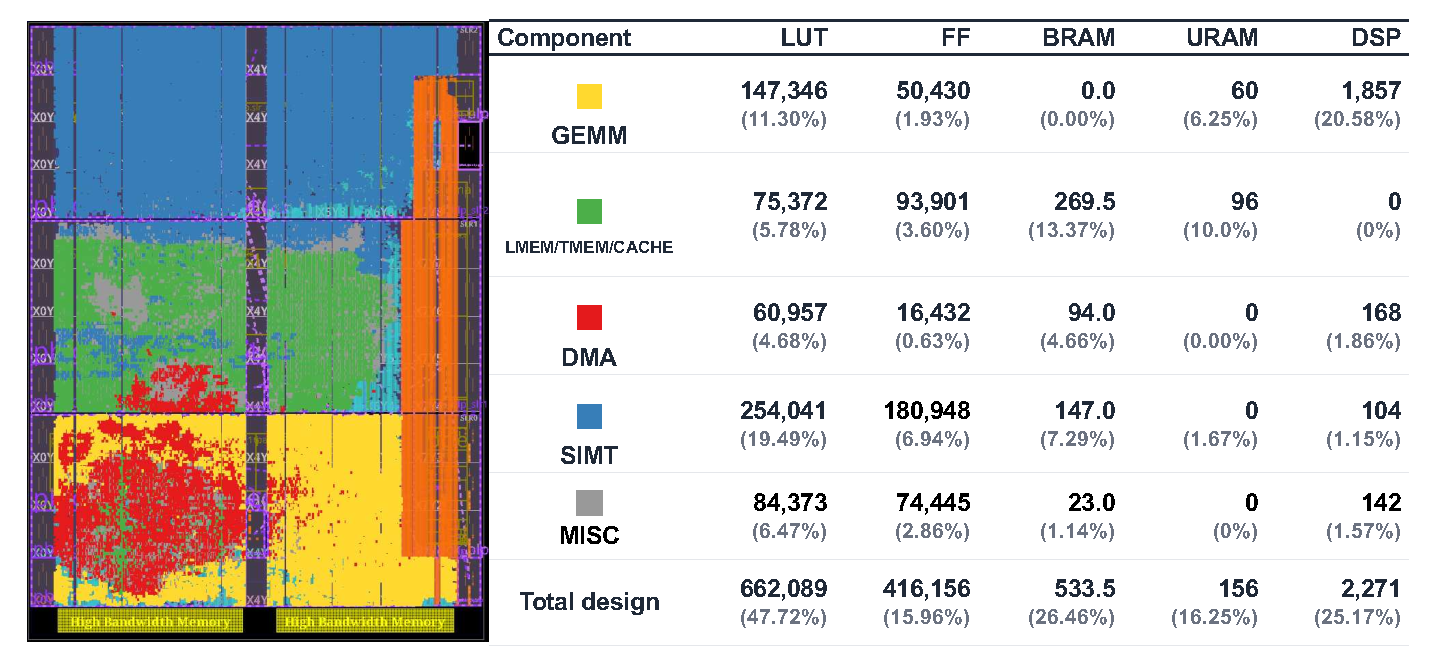
\includegraphics[width=\linewidth]{figures/floorplan.pdf}
    \caption{Floorplan and resource breakdown of \Cfou{} on the Alveo U55C.}
    \label{fig:floorplan}
\end{figure}

All candidates use the same SIMT core, cache hierarchy, and aggregate on-chip memory capacity; Table~\ref{tab:candidates} summarizes the remaining configuration details.

\begin{comment}
Table~\ref{tab:candidates} summarizes the candidate configurations. 
All candidates use one Vortex core with four warps and 32 threads per warp. 
The FP TCU has an $8\times4\times4\times2$ organization, and the \fpint{} GEMM engine uses a $32\times32$ MXU. 
All candidates include a 32~KiB L1 instruction cache and 32~KiB L1 data cache. 
C1--C3 provide 1~MiB of local memory. C4 partitions the same 1~MiB aggregate on-chip storage capacity into 512~KiB of local memory, 256~KiB of TMEM, and 256~KiB of accumulator memory.
\end{comment}

\begin{table}[t]
\centering
\caption{Hardware candidates used in the evaluation.}
\label{tab:candidates}
\scriptsize
\setlength{\tabcolsep}{1pt}
\begin{tabular*}{\columnwidth}{@{\extracolsep{\fill}}*{11}{c}@{}}
\toprule
ID
& \shortstack{Cores}
& \shortstack{Warps}
& \shortstack{Threads}
& \shortstack{FP TCU}
& \shortstack{\fpint{}\\MXU}
& \shortstack{D-cache}
& \shortstack{LMEM}
& \shortstack{TMEM}
& \shortstack{ACC\\MEM}
& \shortstack{Area\\(mm$^2$)} \\
\midrule
C1 & 1 & 4 & 32 & $8\times4\times8$ & -- & 32K & 2M & -- & -- & 10.13 \\
C2 & 1 & 4 & 32 & $8\times4\times8$ & $32\times32$ & 32K & 1.5M & -- & 512K & 12.07 \\
C3 & 1 & 4 & 32 & -- & $32\times32$ & 32K & 1.5M & -- & 512K & 11.52 \\
C4 & 1 & 4 & 32 & -- & $32\times32$ & 32K & 1M & 512K & 512K & 11.21 \\
\bottomrule
\end{tabular*}
\end{table}

\begin{figure*}[t]
    \centering

    \begin{subfigure}[t]{0.49\textwidth}
        \centering
        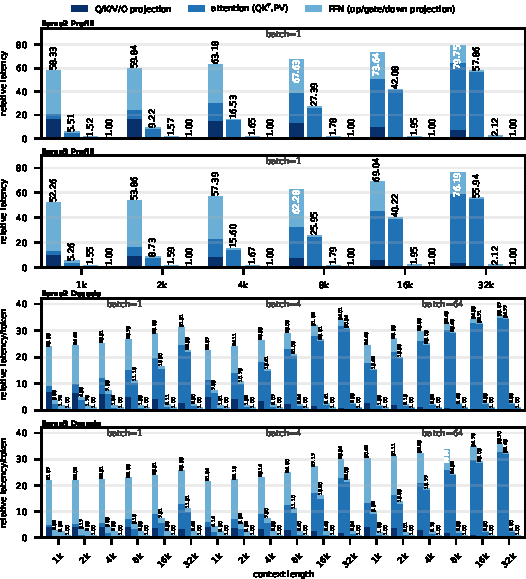
\includegraphics[width=\linewidth]
        {figures/llama2_3/figure_output.C3_C4_v3/llama_gemm_only_no_area_norm/llama_gemm_only_latency_no_area_norm.pdf}
        \caption{GEMM-only latency.}
        \label{fig:gemm-latency}
    \end{subfigure}
    \hfill
    \begin{subfigure}[t]{0.49\textwidth}
        \centering
        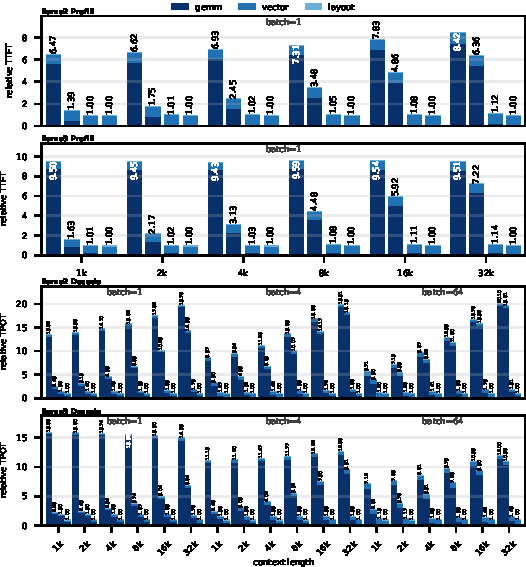
\includegraphics[width=\linewidth]
        {figures/llama2_3/figure_output.C3_C4_v3/llama_e2e_no_area_norm_stacked/llama_e2e_latency_no_area_norm_stacked.pdf}
        \caption{End-to-end system-level TTFT/TPOT.}
        \label{fig:e2e-latency-gemm-layout-vector}
    \end{subfigure}

    \caption{Latency comparison across C1--C4: (a) GEMM-only latency and
    (b) system-level time to first token (TTFT)/time per output token (TPOT). For each workload, the four bars from left
    to right represent C1--C4, with values normalized to C4.}
    \label{fig:llama-relative-latency}
\end{figure*}

Beyond the differences in on-chip SRAM composition summarized in Table~\ref{tab:candidates}, C3 and C4 differ in how the same GEMM ports connect to on-chip SRAM.
Both C3 and C4 use 64\,B I/W/SZ/O GEMM ports. In C3, these ports access 8\,B local memory (LMEM) banks through 64-to-8\,B gather/scatter logic; together with the LMEM crossbar and arbitration, this path incurs roughly 20 cycles of access latency. In C4, each 64\,B GEMM port instead connects to the TMEM banks through a 64\,B-wide mux/demux that supports aligned transfers, providing one-cycle access. For transfers between HBM and on-chip SRAM, C3’s DMA traverses the baseline Vortex cache hierarchy at 64\,B/cycle, whereas C4 bypasses the cache and uses an interleaved HBM–TMEM connection that provides 512\,B/cycle.

\textbf{Latency/Power/Area Measurement Methodology.}
All latency results come from placed-and-routed designs on a Xilinx Alveo U55C FPGA at 100\,MHz. Fig.~\ref{fig:floorplan} shows the floorplan of the complete design. Each candidate runs the same \wkv{}-quantized model and differs only in how GEMMs and tensor movement map to hardware.

We sample FPGA-board power with \texttt{xrt-smi} during kernel execution and subtract idle power from the mean of the samples to obtain dynamic power. Per-kernel dynamic energy is computed from dynamic power and measured latency; end-to-end latency and energy are obtained by summing the corresponding per-kernel values. Energy per token is the end-to-end dynamic energy divided by the number of processed tokens.
To model fused dequantization, we assign it no standalone latency, which is optimistic for the baseline: state-of-the-art fused kernels such as Marlin\cite{marlin} and BitDecoding\cite{bitdecoding} hide most, but not all, of this latency. Its energy component likewise includes only the conversion arithmetic executed on the SIMT lanes. We obtain it by measuring a materializing dequantization kernel on the same tensors and subtracting the HBM-access, address-generation, and control energy, so that no intermediate tensor traffic is charged to the baseline.

% For area estimation, we synthesize the FP TCU and \fpint{} GEMM engine using Synopsys Design Compiler at 100\,MHz in a 28\,nm technology since it is not straightforward to compare the area using FPGA implementation. The candidate-specific area includes the FP TCU, the \fpint{} GEMM engine, the DMA engines, and interconnect control logic, including arbitration. We exclude the common SIMT datapath and the on-chip SRAM area because the SIMT organization and aggregate on-chip SRAM capacity are identical across all candidates.
\begin{comment}
Because FPGA resource counts do not translate directly into area, we synthesize the FP TCU and \fpint{} GEMM engine with Synopsys Design Compiler at 100\,MHz in 28\,nm.
The candidate-specific area covers the FP TCU, the \fpint{} GEMM engine, the DMA engines, and interconnect control logic including arbitration. 
It excludes the common SIMT datapath and on-chip SRAM, whose organization and aggregate capacity are identical across candidates.
\end{comment}
Because FPGA resource counts do not directly translate into silicon area, we synthesize each candidate's complete top-level logic with Synopsys Design Compiler at 100\,MHz in a 28\,nm CMOS technology, including the compiled SRAM macro area.
The total area includes the SIMT datapath, FP TCU, \fpint{} GEMM engine, DMA engines, SRAM macros, and interconnect and arbitration logic (Table~\ref{tab:candidates}).
All candidates maintain the same aggregate on-chip SRAM capacity. For each SRAM bank, we select the closest matching compiled macro based on the required capacity, width, and port configuration, so that the reported area reflects the actual SRAM organization rather than a capacity-based estimate. C2 is the largest because it includes both the FP TCU and FP-INT MXU and separately provisions LMEM and ACC MEM, resulting in less area-efficient SRAM macro configurations. C3 is smaller than C2 because it eliminates the FP TCU. Although C4 further partitions LMEM into ACC MEM and TMEM, the resulting banks map to compiled macros with similar area efficiency, incurring negligible SRAM area overhead. C4 is therefore smaller than C3 because its aligned tensor path simplifies the DMA engines and surrounding interconnect logic, while delivering higher bandwidth than C3.
%All SRAMs are mapped to high-density macros from the same memory library.

%All candidates hold the aggregate on-chip SRAM capacity constant, but the synthesized area reflects each candidate's actual macro, bank, and port configuration rather than scaling with capacity alone (Table~\ref{tab:candidates}). C2 is largest because it includes both the FP TCU and FP-INT MXU, while C3 omits the former. C4 uses finer SRAM partitioning than C3 but remains smaller, as its aligned tensor path requires less DMA logic.
\begin{comment}
For candidate $i$, we multiply its measured FPGA latency $L_i$ by its synthesized total area $A_i$ and normalize the product to C4 for each workload. We refer to the resulting ratio, $(A_iL_i)/(A_{\mathrm{C4}}L_{\mathrm{C4}})$, as area-normalized latency throughout the evaluation.
\end{comment}
%For candidate $i$, we multiply its measured FPGA latency $L_i$ by its synthesized total area $A_i$ and normalize the product to C4 for each workload. We refer to the resulting ratio, $(A_iL_i)/(A_{\mathrm{C4}}L_{\mathrm{C4}})$, as the area--latency metric throughout the evaluation.

\begin{comment}
% sram macro 까지 포함하는 경우
Because FPGA resource counts do not translate directly into area, we synthesize the FP TCU and \fpint{} GEMM engine with Synopsys Design Compiler at 100\,MHz in 28\,nm.
The candidate-specific area covers the FP TCU, the \fpint{} GEMM engine, the DMA engines, sram macros, and interconnect control logic including arbitration. 
It excludes the common SIMT datapath, whose organization is identical across candidates.
\end{comment}

\begin{comment}
% 전체 top으로 하는 경우.
Because FPGA resource counts do not directly translate to silicon area, we synthesize each candidate’s logic with Synopsys Design Compiler at 100 MHz in a 28 nm technology and add the areas of its instantiated SRAM macros. 
All SRAMs are mapped to high-speed macros from the same memory library.
The total area includes the SIMT datapath, FP TCU, FP-INT GEMM engine, DMA engines, SRAM macros, and interconnect and arbitration logic.
\end{comment}

\textbf{Workloads.}
We evaluate prefill, decode, and end-to-end inference for Llama2-7B\cite{llama2} and Llama3-8B\cite{llama3}. We evaluate decode at batch sizes 1, 4, and 64 with context lengths from 1K to 32K. Each run generates 128 output tokens, and the reported latency and energy are averaged per generated token. Both models are quantized with INT4 weights, an INT4  KV cache, and FP16 input using SpinQuant W4A16KV4 quantization\cite{liu2024spinquant}. Under this scheme, $QK^T$ maps to Q-COL and $PV$ maps to Q-ROW, so both execution modes of the proposed MXU are exercised (Table~\ref{tab:kv_quant_direction}). The implementation includes all vector kernels required by SpinQuant, including the Hadamard transforms. GEMMs execute on the FP TCU and/or \fpint{} GEMM engine available in each candidate. In C4, vector kernels adjacent to GEMMs fuse the required layout transformation rather than invoking a standalone kernel.

%\textbf{Software implementation.}
% ---------------------------------------------------------------------
% The host and kernel code use the Vortex runtime, and all device kernels are implemented natively in C++ for Vortex. Vector operations follow an Single-Program Multiple-Data (SPMD) execution model. 
% GEMMs invoke either the Vortex FP TCU kernels or the \fpint{} GEMM engine through MMIO-programmed descriptors. 
% %A native kernel programs the matrix dimensions, INT-operand orientation, quantization direction, and related metadata, launches the GEMM operation, and polls an MMIO status register for completion. Execution order, descriptor construction, and layout handling are expressed directly in the kernels and runtime.

% All candidates use the same sequential attention schedule. The $QK^T$ GEMM writes the attention-score tensor to HBM, after which a standalone Vortex SIMD kernel computes online softmax and writes its result back to HBM for the following $PV$ GEMM. Here, online softmax refers to the algorithm used within the standalone SIMD kernel; we do not fuse $QK^T$, softmax, and $PV$ into a single tiled attention kernel. The reported latency and energy include these vector kernels and intermediate HBM transfers. This common schedule isolates differences in GEMM execution and operand delivery while evaluating each candidate within an end-to-end LLM inference flow rather than as a bare GEMM microbenchmark.
% ---------------------------------------------------------------------
% +++++++++++++++++++++++++++++++++++++++++++++++++++++++++++++++++++++
\textbf{Software implementation.} The host and device code use the Vortex runtime, with all kernels implemented natively in C++. Vector operations follow a single-program multiple-data (SPMD) model, and GEMMs invoke either the Vortex FP TCU kernels or the \fpint{} GEMM engine through MMIO-programmed descriptors.

%All candidates share the same sequential attention schedule: the $QK^T$ GEMM writes the score tensor to HBM, a standalone Vortex SIMD kernel computes online softmax and writes it back, and the following $PV$ GEMM consumes it. We do not fuse $QK^T$, softmax, and $PV$ into a single tiled kernel, and the reported latency and energy include these vector kernels and their intermediate HBM transfers. This common schedule isolates differences in GEMM execution and operand delivery while keeping each candidate within a full inference flow rather than a bare GEMM microbenchmark.
% +++++++++++++++++++++++++++++++++++++++++++++++++++++++++++++++++++++

\subsection{GEMM-Only Latency}

We first isolate the GEMM portion of inference to see how each architectural change affects the compute path and the memory system feeding it. The GEMM-only results sum the Q/K/V/O projections, the $QK^T$ and $PV$ attention GEMMs, and the FFN projections, excluding vector kernels and their fused layout work. %Within each workload, the minimum candidate value is normalized to one.

%The candidate sequence provides three controlled comparisons. C1--C2 tests whether native \fpint{} execution limited to linear layers is sufficient. C2--C3 measures the additional benefit of moving $QK^T$ and $PV$ to the native \fpint{} datapath. C3--C4 compares the same \fpint{} arithmetic coverage and MXU size under the conventional Vortex operand-delivery path and the complete FINISH tensor-memory and software stack. The C3--C4 comparison therefore measures the joint contribution of TMEM, the direct tensor paths, specialized DMA engines, and the compatible tensor layout.

% \begin{figure}[t]
%     \centering
%     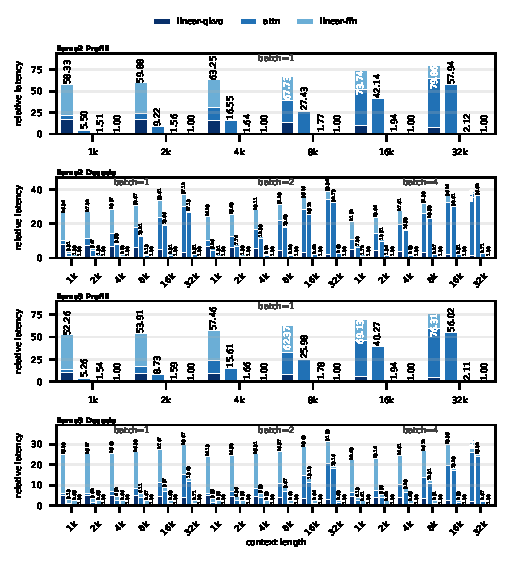
\includegraphics[width=\columnwidth]{figures/llama2_3/figures_script/llama_gemm_only_no_area_norm/llama_gemm_only_latency_no_area_norm.pdf}
%     \caption{Relative GEMM-only latency without area normalization. Within each workload, the four bars from left to right represent C1--C4. Values are normalized to C4. 
%     %Colors group the Q/K/V/O projections, the $QK^T$ and $PV$ attention GEMMs, and the FFN projections.
%     }
%     \label{fig:gemm-latency-no-area-norm}
% \end{figure}
\begin{comment}
\begin{figure*}[t]
    \centering
    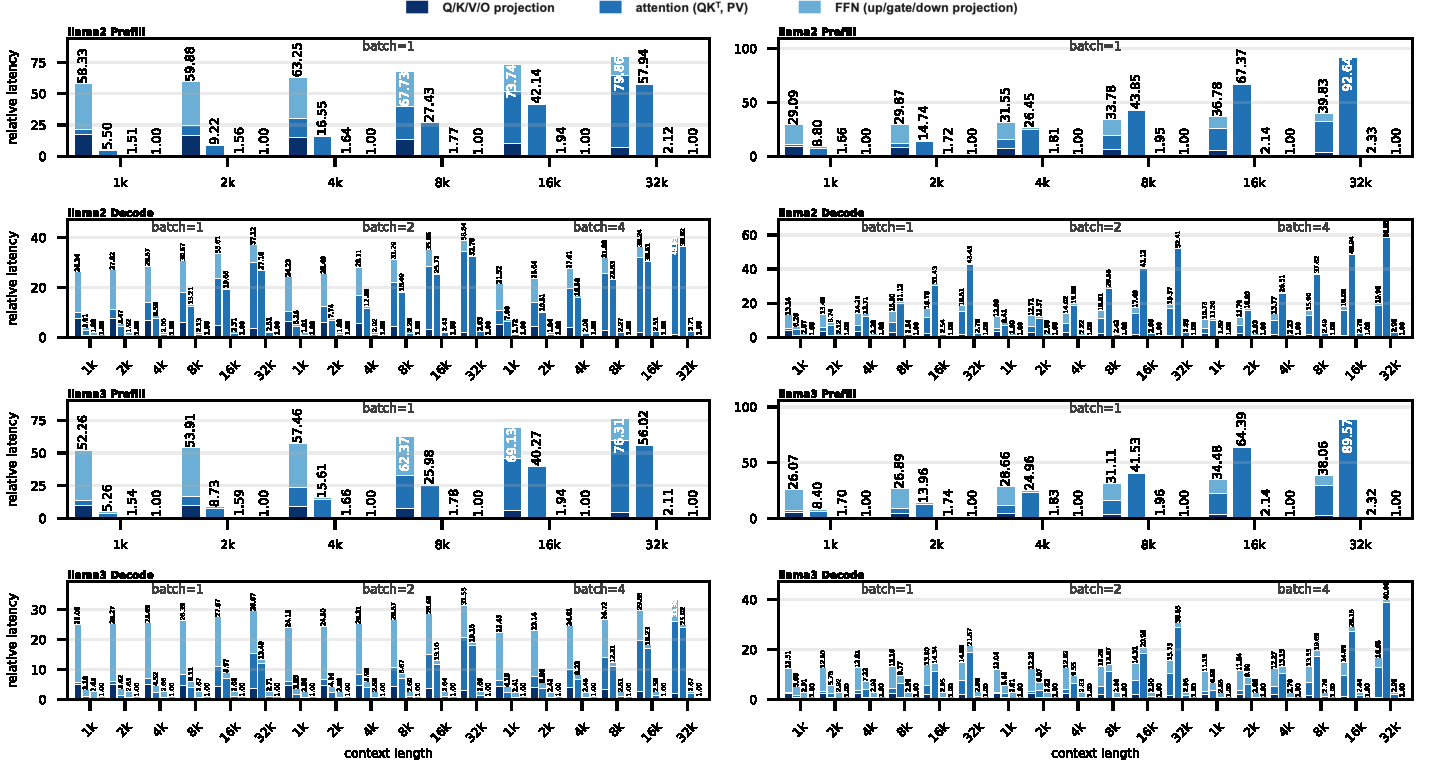
\includegraphics[width=\textwidth]{figures/gemm_only_integrated.pdf}
    \caption{GEMM-only latency without (left) and with (right) area normalization. For each workload, the four bars from left to right represent C1--C4, with values normalized to C4.}
    \label{fig:gemm-latency}
\end{figure*}
\end{comment}



% \begin{figure}[t]
%     \centering
%     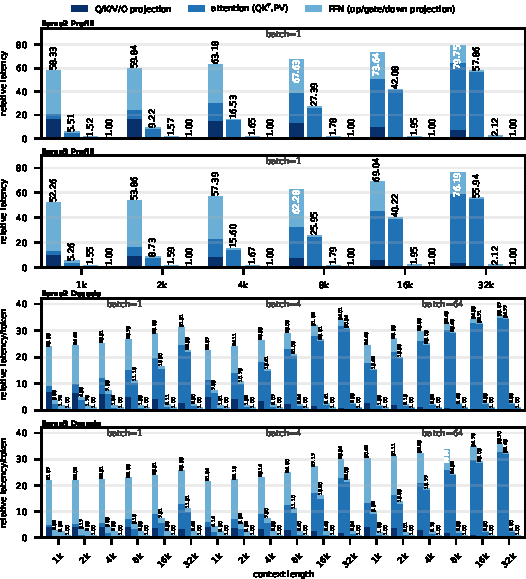
\includegraphics[width=\columnwidth]{figures/llama2_3/figure_output.C3_C4_v3/llama_gemm_only_no_area_norm/llama_gemm_only_latency_no_area_norm.pdf}
%     \caption{Relative GEMM-only latency. For each workload, the four bars from left to right represent C1--C4, with values normalized to C4.}
%     \label{fig:gemm-latency}
% \end{figure}

\begin{comment}
\textbf{Raw latency.}
Figure~\ref{fig:gemm-latency} (left) reports measured FPGA latency without area normalization. Relative to C1, C4 reduces geometric-mean GEMM latency by $63.97\times$ in prefill and $28.20\times$ in decode. C2 reduces latency over C1 by $3.35\times$ and $2.74\times$, respectively, by moving the linear projections to the larger \fpint{} MXU, but it continues to execute $QK^T$ and $PV$ on the FP TCU. Moving these attention GEMMs to the native \fpint{} datapath in C3 reduces latency over C2 by a further $10.91\times$ in prefill and $4.37\times$ in decode. C4 then reduces latency over C3 by another $1.75\times$ and $2.35\times$, respectively, while using the same MXU and the same native \fpint{} coverage.
\end{comment}

%These comparisons expose two successive system bottlenecks. C2 is limited by the FP attention fallback, which becomes increasingly important as the attended sequence grows. C3 removes this fallback but continues to feed the larger MXU through a general-purpose, misalignment-tolerant memory path. C4 addresses the latter bottleneck through the combined use of aligned tile-major transfers, TMEM bank parallelism, and the higher-bandwidth HBM--TMEM tensor path.

% \begin{figure}[t]
%     \centering
%     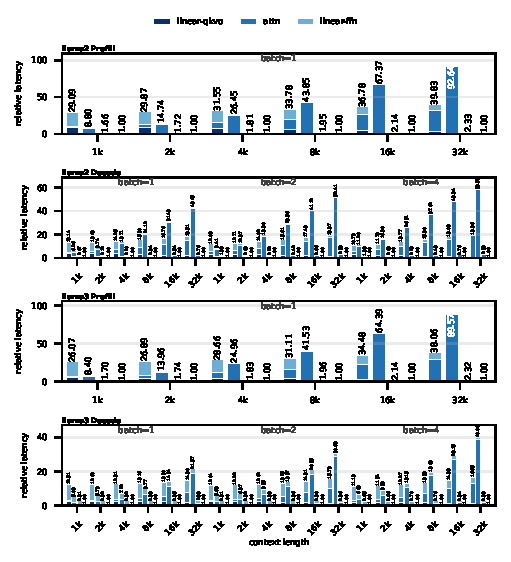
\includegraphics[width=\columnwidth]{figures/llama2_3/figures_script/llama_gemm_only/llama_gemm_only_latency.pdf}
%     \caption{Area-normalized relative GEMM-only latency. Within each workload,
%     the four bars from left to right represent C1--C4. Values are normalized to C4.}
%     \label{fig:gemm-latency-area-norm}
% \end{figure}

%\textbf{Relative latency.}
% \textbf{Area--latency metric.}
\begin{comment}
Figure~\ref{fig:gemm-latency} (right) applies the area--latency metric defined above. C4 reduces the geometric-mean metric over C1 by $31.91\times$ in prefill and $14.06\times$ in decode. Area normalization most strongly affects C2 because it contains both the FP TCU and the \fpint{} MXU. Although C2 improves raw latency in every workload, its geometric-mean area--latency product improves over C1 by only $1.04\times$ in prefill and is $1.17\times$ higher than C1 in decode. C2 has a higher metric than C1 in half of the prefill workloads and in 22 of the 36 decode workloads.

C3 reduces the metric over C2 by $15.85\times$ in prefill and $6.35\times$ in decode by removing the FP attention fallback and the need to provision both compute units. C4 further reduces the metric over C3 by $1.93\times$ and $2.59\times$, respectively. Thus, the performance benefit obtained from the proposed tensor path exceeds the added DMA and interconnect logic cost.
\end{comment}
Fig.~\ref{fig:gemm-latency} shows that C4 reduces the geometric-mean GEMM latency over C1 by $63.90\times$ in prefill and $27.36\times$ in decode. 
%Despite provisioning both compute units, C2 reduces GEMM latency over C1 by $3.35\times$ and $2.22\times$, respectively, by moving the linear projections to the \fpint{} MXU.
Even with both compute units provisioned and the linear projections moved to the \fpint{} MXU, C2 achieves only $3.35\times$ and $2.22\times$ GEMM speedups over C1, respectively.
Accordingly, C2 performs well relative to C1 at short sequence lengths, but this advantage rapidly narrows as the sequence length increases.
At long sequence lengths, the FP attention GEMMs dominate latency, and C2 still executes $QK^T$ and $PV$ on the same slower FP TCU as C1, limiting the benefit of accelerating only the linear projections.
Moving the attention GEMMs to the native \fpint{} datapath in C3 further improves the metric over C2 by $10.86\times$ and $5.52\times$. C4 then improves the metric over C3 by another $1.76\times$ and $2.23\times$, showing that the benefit of the proposed tensor path exceeds its added DMA and interconnect cost.
\begin{comment}
Figure~\ref{fig:gemm-latency} shows that C4 reduces the geometric-mean area-normalized GEMM latency over C1 by $55.20\times$ in prefill and $22.00\times$ in decode. Despite provisioning both compute units, C2 improves area-normalized latency over C1 by $2.81\times$ and $2.33\times$, respectively, by moving the linear projections to the \fpint{} MXU. Moving the attention GEMMs to the native \fpint{} datapath in C3 further improves area-normalized latency over C2 by $11.37\times$ and $4.37\times$. C4 then improves it over C3 by another $1.73\times$ and $2.16\times$, showing that the benefit of the proposed tensor path exceeds its added DMA and interconnect cost.
\end{comment}

\subsection{End-to-End Latency and Data Layout Overhead}

We next analyze the complete inference path: all GEMMs, vector kernels, and fused layout transformations. The breakdown separates these costs into \emph{gemm}, \emph{vector}, and \emph{layout}. The layout portion denotes the incremental work used to produce or consume tile-major tensors inside adjacent fused vector kernels, whereas the vector portion contains the remaining non-GEMM computation.

% \begin{figure}[t]
%     \centering
%     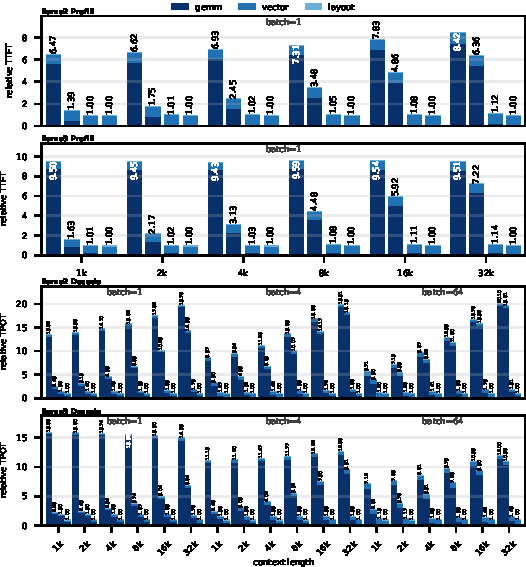
\includegraphics[width=\columnwidth]{figures/llama2_3/figure_output.C3_C4_v3/llama_e2e_no_area_norm_stacked/llama_e2e_latency_no_area_norm_stacked.pdf}
%     \caption{Relative end-to-end latency. For each workload, the four bars from left to right represent C1--C4, with values normalized to C4}
%     \label{fig:e2e-latency-gemm-layout-vector}
% \end{figure}

\begin{comment}
Figure~\ref{fig:e2e-latency-gemm-layout-vector} shows that C4 reduces the geometric-mean area--latency metric over C1 by $2.05\times$ in prefill and $5.20\times$ in decode, with maximum improvements of $2.35\times$ and $7.87\times$, respectively. The same progression observed in the GEMM-only results remains visible: C2 pays for two compute units while retaining the FP attention path, C3 removes this fallback, and C4 provides the lowest metric by combining native \fpint{} execution with the optimized operand-delivery path.
\end{comment}
Fig.~\ref{fig:e2e-latency-gemm-layout-vector} shows that C4 reduces the geometric-mean end-to-end latency over C1 by $8.29\times$ in prefill and $12.43\times$ in decode, with maximum improvements of $9.59\times$ and $20.10\times$, respectively. The same progression observed in the GEMM-only results remains visible: C2 pays for two compute units while retaining the FP attention path, C3 removes this fallback, and C4 provides the lowest metric by combining native \fpint{} execution with the optimized operand-delivery path.
\begin{comment}
Figure~\ref{fig:e2e-latency-gemm-layout-vector} shows that C4 reduces the geometric-mean area-normalized end-to-end latency over C1 by $7.22\times$ in prefill and $11.61\times$ in decode, with maximum improvements of $8.35\times$ and $17.02\times$, respectively. The same progression observed in the GEMM-only results remains visible: C2 pays for two compute units while retaining the FP attention path, C3 removes this fallback, and C4 provides the lowest area-normalized latency by combining native \fpint{} execution with the optimized operand-delivery path.
\end{comment}

% The end-to-end improvements are smaller than the GEMM-only improvements because all candidates execute the same vector kernels and materialize the same intermediate attention tensors in HBM. In particular, the C4-over-C3 improvement is $1.02\times$ in prefill and $1.55\times$ in decode. The prefill gain is modest because vector kernels constitute a larger fraction of the remaining latency after the GEMMs are accelerated. Decode retains more of the GEMM-path improvement because its non-GEMM vector work occupies a smaller fraction of end-to-end execution. The explicit layout segment remains limited across the evaluated workloads, showing that C4 retains its end-to-end benefit after accounting for fused tile-major conversion.
\begin{comment}
The end-to-end improvements are smaller than the GEMM-only ones because all candidates run the same vector kernels and materialize the same intermediate attention tensors in HBM: the C4-over-C3 gain is $1.02\times$ in prefill and $1.55\times$ in decode. Prefill gains less because, once the GEMMs are accelerated, vector kernels dominate the remaining latency, whereas decode retains more of the GEMM-path improvement. The explicit layout segment stays small across workloads, so C4 keeps its end-to-end benefit even after accounting for fused tile-major conversion.
\end{comment}
The end-to-end improvements are smaller than the GEMM-only ones because all candidates run the same vector kernels and materialize the same intermediate attention tensors in HBM: the C4-over-C3 gain is $1.06\times$ in prefill and $1.54\times$ in decode. %The gain in prefill is smaller than decode case because, once the GEMMs are accelerated, vector kernels dominate the remaining latency, whereas decode retains more of the GEMM-path improvement. 
The latency due to layout overhead remains small across workloads, so C4 keeps its end-to-end benefit even after accounting for fused tile-major conversion.

\subsection{Dynamic Power and Energy}

\textbf{Dynamic power.}
\begin{comment}
Table~\ref{tab:kernel-dynamic-power} summarizes the dynamic FPGA-board power used in the energy calculation. Non-quantization vector kernels draw 0.89--2.11~W across their measured means. The three GEMM paths span 1.76--2.31~W: the optimized \fpint{} GEMM draws 2.00~W, compared with 2.31~W for the naive \fpint{} path and 1.76~W for the FP TCU. These power differences are substantially smaller than the corresponding latency differences, making execution time the dominant source of energy variation among the candidates.
\end{comment}
Table~\ref{tab:kernel-dynamic-power} summarizes the dynamic FPGA-board power used in the energy calculation.
%Non-quantization vector kernels draw 0.89--2.11~W across their measured means. The three GEMM paths span 1.69--1.96~W: the optimized \fpint{} GEMM draws 1.71~W, compared with 1.96~W for the naive \fpint{} path and 1.69~W for the FP TCU.
These power differences are substantially smaller than the corresponding latency differences, making execution time the dominant source of energy variation among the candidates.

\begin{table}[t]
    \centering
    \caption{Dynamic FPGA board power (W).}
    \label{tab:kernel-dynamic-power}
    %\scriptsize
    \setlength{\tabcolsep}{1.3pt}
    \begin{tabular*}{\columnwidth}
        {@{\extracolsep{\fill}}lrlr@{}}
        \toprule
        Kernel & Power & Kernel & Power \\
        \midrule
        Vector kernels & $0.89$--$2.11$
            & FP$\times$FP GEMM & $1.69 \pm 0.52$ \\
        Quant. & $1.21 \pm 0.71$
            & FP--INT GEMM (naive) & $1.96 \pm 0.78$ \\
        Dequant. & $1.25 \pm 0.10$
            & FP--INT GEMM (optimized) & $1.71 \pm 0.61$ \\
        \bottomrule
    \end{tabular*}
\end{table}

\textbf{End-to-end energy.}
% We next evaluate whether the latency improvements translate into lower dynamic energy. End-to-end energy includes GEMM execution, dequantization, fused layout work, vector kernels, and the intermediate HBM transfers exercised by the common attention schedule.
End-to-end energy sums GEMM execution, dequantization, fused layout work, vector kernels, and the intermediate HBM transfers of the common attention schedule.
\begin{figure}[t]
    \centering
    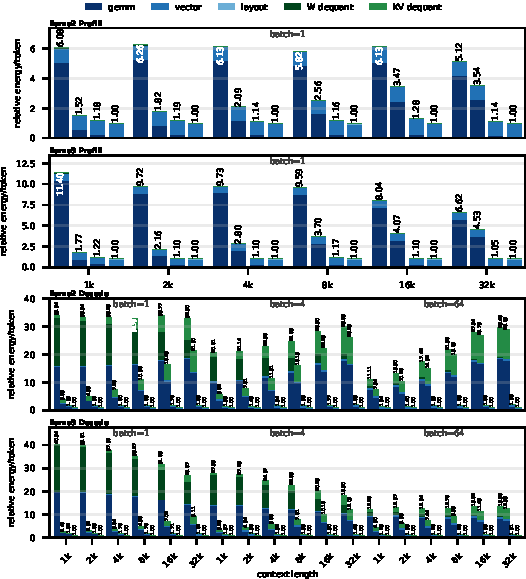
\includegraphics[width=\columnwidth]{figures/llama2_3/figure_output.C3_C4_v3/llama_energy_no_area_norm_gemm_layout_vector_stacked/llama_energy_per_token_power_dynamic_avg_W_no_area_norm_gemm_layout_vector_stacked.pdf}
    \caption{End-to-end energy per token. For each workload, the four bars from left to right represent C1--C4, with values normalized to C4.}
    %\caption{End-to-end energy per token computed from raw measured FPGA latency and idle-subtracted dynamic board power. Within each workload, the  four bars from left to right represent C1--C4, and the minimum candidate energy is normalized to one. The stacks separate GEMM, fused layout  transformation, common vector execution, and dequantization. No area normalization is applied.}
    \label{fig:e2e-energy-dequant-breakdown}
\end{figure}
\begin{comment}
Figure~\ref{fig:e2e-energy-dequant-breakdown} shows that C4 reduces geometric-mean end-to-end energy over C1 by $3.85\times$ in prefill (up to $6.32\times$). In decode the geometric-mean and maximum reductions grow to $97.44\times$ and $201.91\times$, because C1 and C2 dequantize the entire KV cache at every step whereas prefill consumes freshly generated K and V directly and dequantizes no existing cache.
\end{comment}
\begin{comment}
Figure~\ref{fig:e2e-energy-dequant-breakdown} shows that C4 reduces geometric-mean end-to-end energy over C1 by $6.65\times$ in prefill (up to $11.17\times$). In decode the geometric-mean and maximum reductions grow to $47.77\times$ and $66.74\times$, because C1 and C2 dequantize the entire KV cache at every step whereas prefill consumes freshly generated K and V directly and dequantizes no existing cache.
\end{comment}
Fig.~\ref{fig:e2e-energy-dequant-breakdown} shows that C4 reduces geometric-mean energy per token over C1 by $7.31\times$ in prefill. In decode the geometric-mean energy reduction grows to $23.33\times$, because C1 and C2 dequantize the entire KV cache at every step whereas prefill consumes freshly generated K and V directly and dequantizes no existing cache. This widening gap highlights the importance of end-to-end native \fpint{} execution, which avoids repeatedly dequantizing the growing KV cache during decode.
%The dequantization segment for C1 in prefill consists only of static 4-bit weight conversion; C2--C4 consume the quantized weights directly for their linear layers.

%Decode has a different cost structure. Each step produces only one new token, but $QK^T$ and $PV$ consume the K and V entries accumulated over the preceding context. C1 and C2 execute these attention GEMMs on the FP TCU and therefore dequantize all consumed KV-cache entries at every step. Across the decode workloads, dequantization accounts for an average of 88.7\% and 77.4\% of the total energy of C1 and C2, respectively. C1 includes both weight and KV-cache dequantization, whereas C2's dequantization component consists only of the KV-cache conversion.

%C2 therefore isolates the attention-side conversion cost: its linear projections already execute on the native \fpint{} MXU, but $QK^T$ and $PV$ remain on the FP TCU. Consequently, C2 consumes $13.35\times$ more decode energy than C3 on geometric mean and up to $53.95\times$ more. C3 and C4 eliminate this repeated conversion by consuming the quantized K and V operands directly in the native \fpint{} attention path. These results show that linear-only \fpint{} acceleration cannot realize the decode-energy benefit of WKV quantization when attention continues to use an FP datapath.


\subsection{Numerical and Neural Network Accuracy}

% \begin{table*}[t]
% \centering
% \caption{Zero-shot accuracy (\%) on eight downstream tasks and WikiText-2
% perplexity (PPL) for Llama2-7B SpinQuant W4A16KV4\cite{wikitext}.}
% \label{tab:accuracy}

% \scriptsize
% \setlength{\tabcolsep}{1.5pt}
% \begin{tabularx}{\textwidth}{@{}>{\raggedright\arraybackslash}p{0.18\textwidth}YYYYYYYYY|Y@{}}
% \toprule
% & ARC-c & ARC-e & BoolQ & HellaSwag & OBQA & PIQA & SocialQA & WinoG & Avg. $\uparrow$ & PPL $\downarrow$ \\
% \midrule
% GPU reference
% & 44.20 & 73.15 & 76.85 & 75.35 & 42.60 & 78.56 & 45.24 & 68.82 & 63.10 & 5.59 \\
% \fpint{}: linear only
% & 44.37 & 72.98 & 76.24 & 75.34 & 43.20 & 78.40 & 45.29 & 69.22 & 63.13 & 5.59 \\
% \fpint{}: attention only
% & 44.03 & 73.32 & 76.82 & 75.23 & 43.20 & 78.56 & 44.73 & 68.19 & 63.01 & 5.59 \\
% \rowcolor{gray!12}
% \fpint{}: linear and attention
% & 44.03 & 73.02 & 77.13 & 75.22 & 44.20 & 78.78 & 45.24 & 69.53 & 63.39 & 5.59 \\
% \bottomrule
% \end{tabularx}
% \end{table*}
\begin{figure}[t]
    \centering
    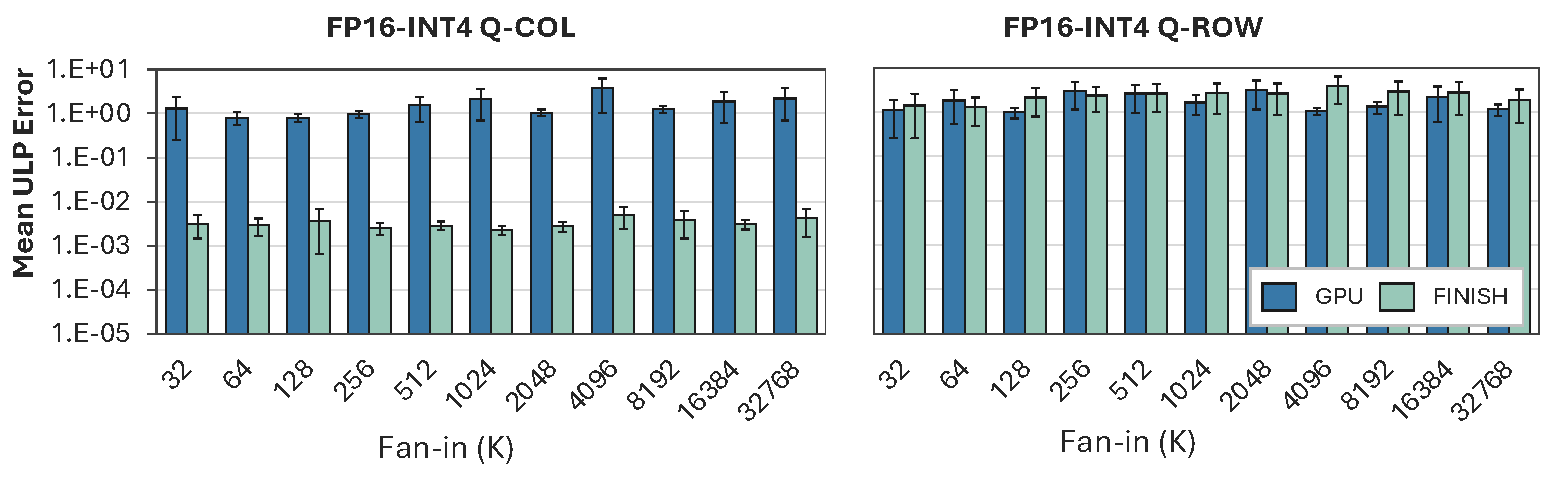
\includegraphics[width=\columnwidth]{figures/fig_num_error.pdf}
    % 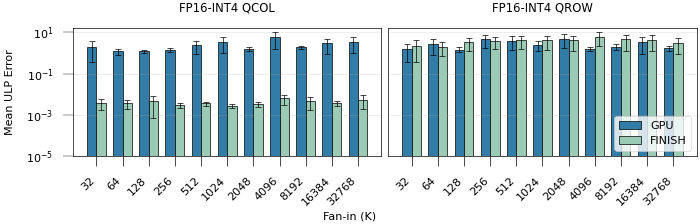
\includegraphics[width=\columnwidth]{figures/numerical_acc/fp16_int4_real2scomp_fanin.png}
    \caption{Mean ULP error of Q-COL and Q-ROW \fpint{} GEMM outputs
against an FP64 reference run on CPU.}
    \label{fig:numerical_accuracy}
\end{figure}

\begin{table}[t]
\centering
\caption{Zero-shot accuracy (\%) and WikiText-2 perplexity for
Llama2-7B and Llama3-8B SpinQuant W4A16KV4~\cite{wikitext}.}
\label{tab:accuracy}

\setlength{\tabcolsep}{1.7pt}
\renewcommand{\arraystretch}{1.05}

\begin{tabular}{@{}lccccccc|c@{}}
\toprule
& \rotatebox{60}{ARC-c}
& \rotatebox{60}{ARC-e}
& \rotatebox{60}{BoolQ}
& \rotatebox{60}{Hella.}
& \rotatebox{60}{OBQA}
& \rotatebox{60}{WinoG}
& \rotatebox{60}{Avg.$\uparrow$}
& \rotatebox{60}{PPL$\downarrow$} \\
\midrule

\multicolumn{9}{@{}l}{\textit{Llama2-7B}} \\
GPU ref.
& 44.20 & 73.15 & 76.85 & 75.35
& 42.60 & 68.82 & 63.50 & 5.59 \\

\fpint{}: linear
& 44.37 & 72.98 & 76.24 & 75.34
& 43.20 & 69.22 & 63.56 & 5.59 \\

\fpint{}: attention
& 44.03 & 73.32 & 76.82 & 75.23
& 43.20 & 68.19 & 63.47 & 5.59 \\

\rowcolor{gray!12}
\ours{}
& 44.03 & 73.02 & 77.13 & 75.22
& 44.20 & 69.53 & 63.86 & 5.59 \\

\midrule
\multicolumn{9}{@{}l}{\textit{Llama3-8B}} \\
GPU ref.
& 51.11 & 76.98 & 79.27 & 78.11
& 41.80 & 73.16 & 66.74 & 6.47 \\

\fpint{}: linear
& 51.88 & 76.39 & 79.30 & 77.89
& 42.80 & 72.77 & 66.84 & 6.47 \\

\fpint{}: attention
& 51.28 & 76.94 & 78.99 & 78.13
& 43.80 & 73.09 & 67.04 & 6.47 \\

\rowcolor{gray!12}
\ours{}
& 51.62 & 76.94 & 79.36 & 77.98
& 42.20 & 72.53 & 66.77 & 6.47 \\

\bottomrule
\end{tabular}
\end{table}

We evaluate numerical fidelity at the dot-product level and model quality at the neural network level. Q-COL follows the same scale-application order as conventional GPU FP16 execution while retaining the established FIGNA-style computation, and is therefore expected to preserve, or potentially improve upon, its numerical accuracy. In contrast, Q-ROW folds the scale into the FP operand before prealignment, thereby changing the order of finite-precision operations. We therefore examine whether this scale reordering introduces additional arithmetic error or degrades model-level accuracy.
Fig.~\ref{fig:numerical_accuracy} reports the mean ULP error relative to an FP64 reference computed on the CPU for fan-in values $K$ ranging from 32 to 32,768. In Q-ROW, \ours{} achieves mean ULP error comparable to that of the GPU FP16 path, while in Q-COL, its error remains approximately three orders of magnitude lower. These results show that the proposed scale reordering for Q-ROW does not introduce additional dot-product-level numerical error relative to the GPU FP16 baseline.
Table~\ref{tab:accuracy} compares Llama2-7B and Llama3-8B SpinQuant W4A16KV4 under the GPU reference and under native \fpint{} execution for the linear layers, attention GEMMs, or both. 

Regarding the quality at the neural network level, for both Llama2-7B and Llama3-8B, the GPU FP16 baseline and our FINISH system achieve similar average accuracies across the six zero-shot tasks, and yield almost the same WikiText-2 perplexity, consistent with the small numerical differences observed in the dot-product-level ULP analysis.


%We evaluate numerical accuracy at the dot-product level and the neural network accuracy.
%Fig.~\ref{fig:numerical_accuracy} reports the mean ULP error against an FP64 reference run on GPU for the fan-in $K$ values from 32 to 32768.
%\ours{} matches the GPU FP16 path in Q-ROW and stays about three orders of magnitude below it in Q-COL, so native \fpint{} execution is never less accurate than FP16 in either direction.
%Table~\ref{tab:accuracy} compares Llama2-7B and Llama3-8B SpinQuant W4A16KV4 under the GPU reference and under native \fpint{} execution for the linear layers, attention GEMMs, or both. 
%Across the six zero-shot tasks the GPU reference and full native-\fpint{} execution reach 63.50\% and 63.86\% average accuracy at the same 5.59 WikiText-2 perplexity, and the two intermediate mappings stay in the same narrow range, consistent with the ULP measurements.

\subsection{Hardware Efficiency and Area Overhead}
\label{sec:eval-hw-efficiency}

% \begin{figure}[t]
%     \centering
%     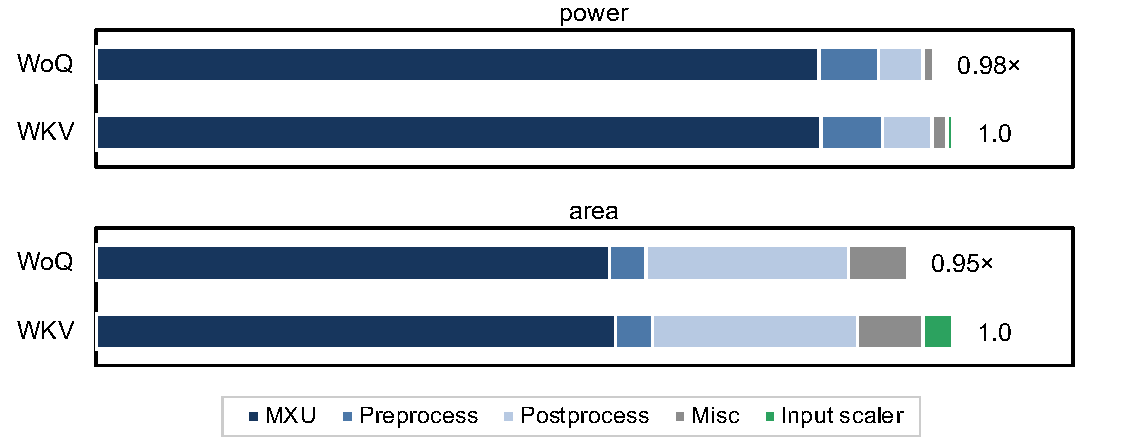
\includegraphics[width=\linewidth]{figures/area_break.pdf}
%     \caption{Power and area breakdown of the weight-only (WoQ) and WKV
%     \fpint{} GEMM engines.}
%     \label{fig:arr-level-break}
% \end{figure}

% \begin{figure}[!t]
%     \centering
%     \begin{subfigure}[t]{\linewidth}
%         \centering
%         % 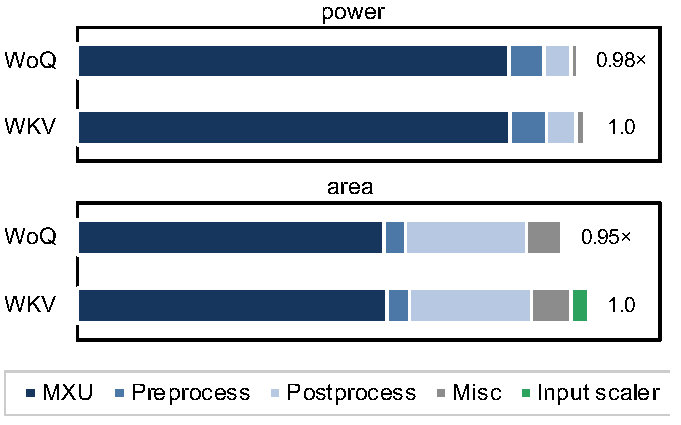
\includegraphics[width=\linewidth]{figures/breakdown_a.pdf}
%         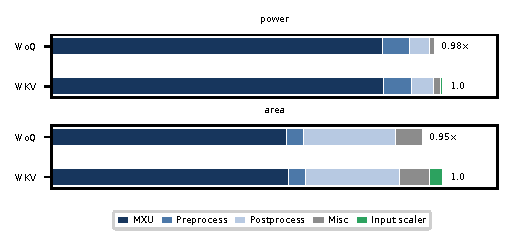
\includegraphics[width=\columnwidth]{figures/gemm_engine_breakdown/fig10_wkv_vs_woq_relative_breakdown.pdf}
%         \caption{WoQ vs.\ WKV GEMM.}
%         \label{fig:arr-level-break}
%     \end{subfigure}
%     \par\medskip
%     \begin{subfigure}[t]{\linewidth}
%         \centering
%         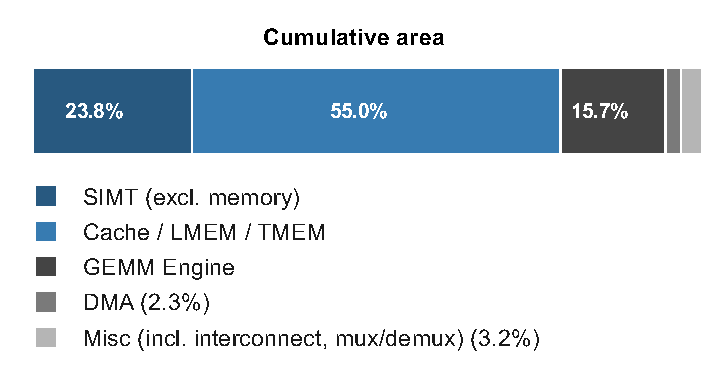
\includegraphics[width=\linewidth]{figures/breakdown_b.pdf}
%         \caption{Full-system breakdown.}
%         \label{fig:area-breakdown}
%     \end{subfigure}
%     \caption{GEMM-engine area and power breakdowns and full-system area breakdown.}
%     \label{fig:area-power-break}
% \end{figure}

\begin{table}[t]
\centering
\caption{Array-level relative efficiency at 28\,nm and 100\,MHz for a
32$\times$32 array, normalized to the FP TCU.}
\label{tab:array-level}
%\small
\setlength{\tabcolsep}{3pt}
\begin{tabularx}{\columnwidth}{@{}>{\raggedright\arraybackslash}Xccc@{}}
\toprule
Unit & Precision & TOPS/mm$^2$ & TOPS/W \\
\midrule
FP TCU & FP$\times$FP & 1.0 & 1.0 \\
WoQ \fpint{} GEMM Engine & \fpint{} & 3.30 & 2.60 \\
WKV \fpint{} GEMM Engine & \fpint{} & 3.13 & 2.54 \\
\bottomrule
\end{tabularx}
\end{table}

% \begin{figure}[t]
%     \centering
%     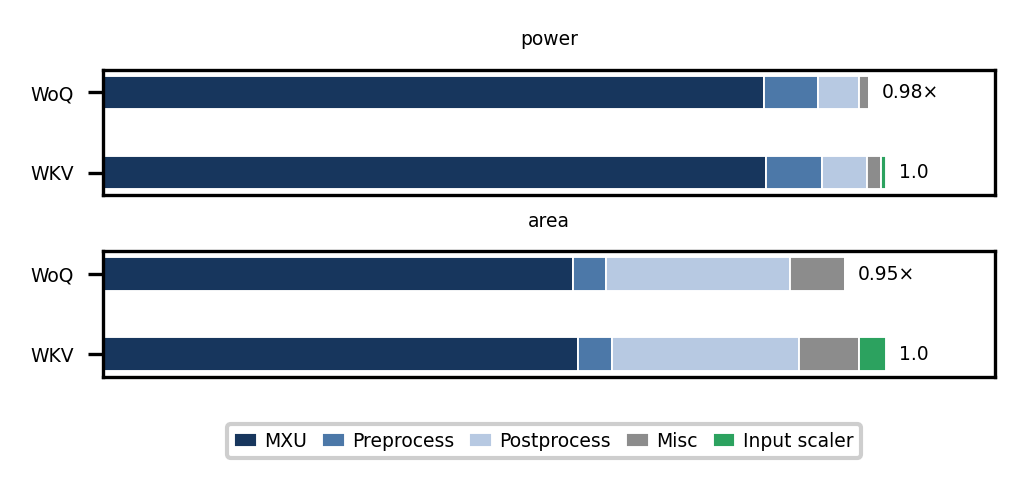
\includegraphics[width=\columnwidth]{figures/gemm_engine_breakdown/fig10_wkv_vs_woq_relative_breakdown.png}
%     \caption{WoQ vs.\ WKV GEMM.}
%     \label{fig:arr-level-break}
% \end{figure}

% \begin{figure}[!t]
%     \centering
%     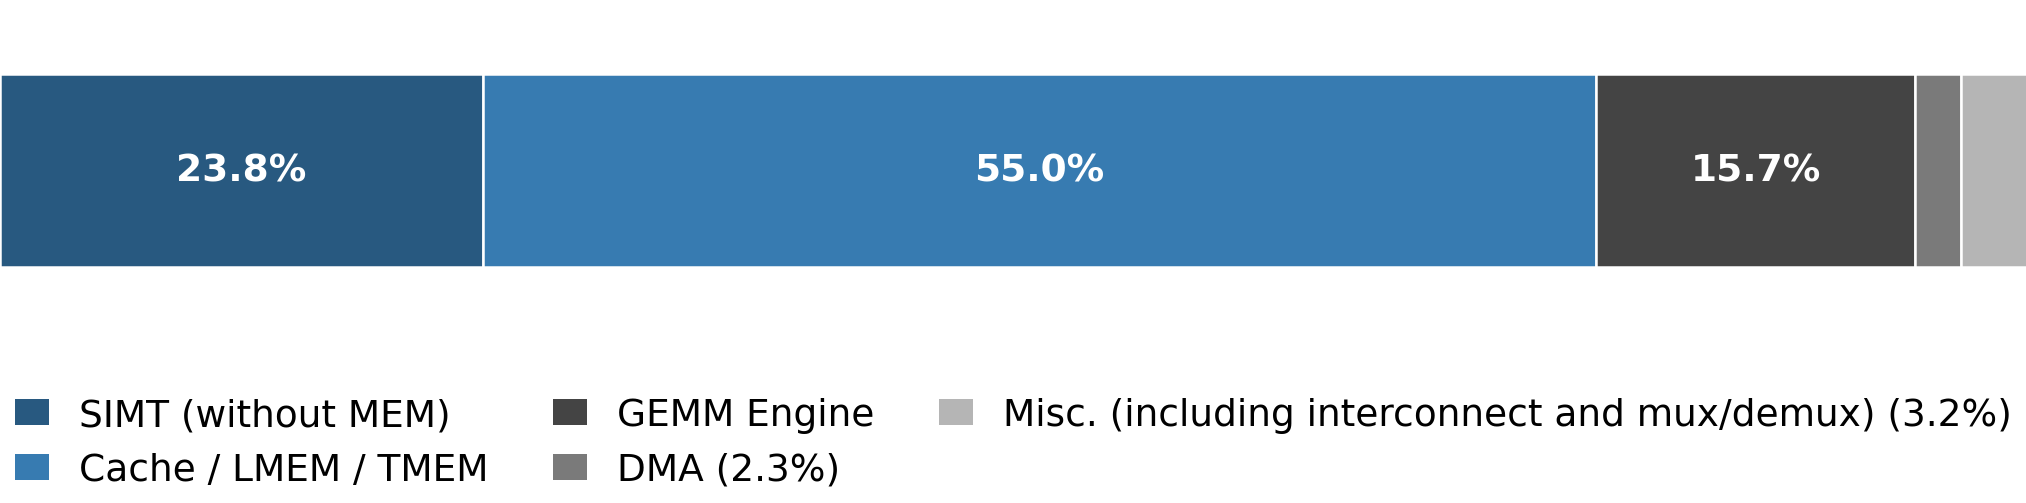
\includegraphics[width=\columnwidth]{figures/top_breakdown/candidate_area_breakdown_hd_c4.png}
%     \caption{Full-system breakdown.}
%     \label{fig:area-breakdown}
% \end{figure}
\begin{figure}[t]
    \centering
    \begin{subfigure}[t]{0.48\columnwidth}
        \centering
        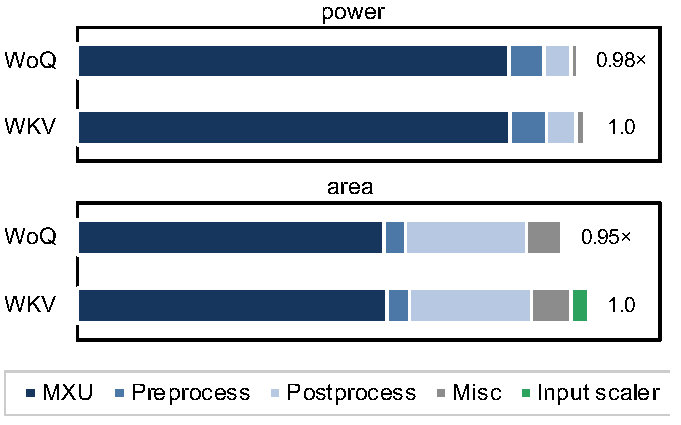
\includegraphics[width=\linewidth]{figures/breakdown_a.pdf}
        \caption{WoQ vs.\ WKV GEMM.}
        \label{fig:arr-level-break}
    \end{subfigure}
    \hfill
    \begin{subfigure}[t]{0.48\columnwidth}
        \centering
        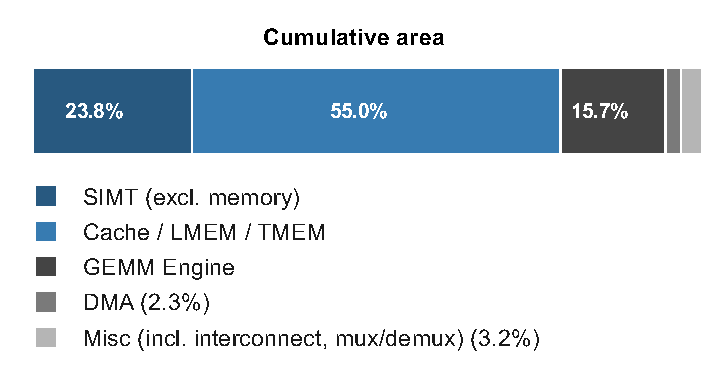
\includegraphics[width=\linewidth]{figures/breakdown_b.pdf}
        \caption{Full-system breakdown.}
        \label{fig:area-breakdown}
    \end{subfigure}
    \caption{Breakdown of the GEMM engine area/power and full system area.}
    \label{fig:breakdown}
\end{figure}

\textbf{Array-level efficiency and attention-support overhead.}
Table~\ref{tab:array-level} shows that the WKV \fpint{} GEMM engine improves TOPS/mm$^2$ by $3.13\times$ and TOPS/W by $2.54\times$ over the FP TCU at the array level.
Compared with the weight-only GEMM engine, adding native support for the KV-attention mappings reduces these efficiencies by only 5.2\% and 2.2\%, respectively, because the area overhead is relatively small.
As shown in Fig.~\ref{fig:arr-level-break}, the additional \qrow{} input scaler accounts for 3.41\% of the WKV GEMM-engine area and 0.60\% of its power.
The overhead remains small because the design shares 32 FP multipliers across the MXU columns instead of placing one multiplier in each of the 1024 processing elements.

\textbf{System-level area overhead.}
Fig.~\ref{fig:area-breakdown} reports the complete system-level area breakdown.
The on-chip memories and the SIMT pipeline excluding memories account for 55.0\% and 23.8\% of the total area, respectively, while the GEMM engine occupies 15.7\%. In contrast, the DMA logic occupies 2.3\%, and the miscellaneous logic including the interconnect and mux/demux occupies 3.2\%. Their combined 5.5\% area contribution shows that the proposed tensor path scales operand bandwidth with relatively small area overhead.

% \begin{figure}[t]
%     \centering
%     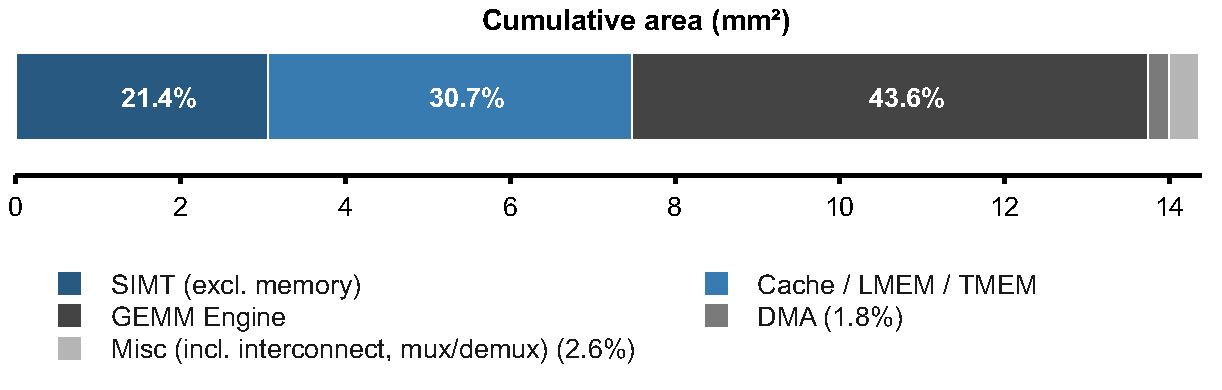
\includegraphics[width=\linewidth]{figures/vortex_break.pdf}
%     \caption{Full-system area breakdown of \ours{}, including the DMA and
%     interconnect overhead of the tensor path.}
%     \label{fig:area-breakdown}
% \end{figure}



\begin{comment}
\section{Evaluation}

\subsection{Methodology}
\textbf{Hardware Evaluation Setup.}
We compare four hardware candidates.

\begin{itemize}
    \item \textit{C1: \Cone{}.}
    Implemented by enabling an FP$\times$FP TCU on Vortex.
    C1 executes all GEMM operations on the FP TCU after
    dequantizing the INT-quantized operands on the SIMT core.

    \item \textit{C2: \Ctwo{}.}
    We add a decoupled \fpint{} MXU on top of C1.
    The QKV generation and the FFN linear projections are
    executed on the \fpint{} MXU, while the $QK^T$ and PV
    operations of attention are executed on the FP TCU.
    C2 represents prior work such as FIGNA/FIGLUT/LUT-TC
    that accelerates only linear operations with \fpint{}.

    \item \textit{C3: \Cthr{}.}
    Both linear layers and the $QK^T$ and PV attention operations execute
    on the \fpint{} MXU, but the memory subsystem, runtime, and tensor
    layout remain unoptimized. C3 minimizes changes to the Vortex memory
    system by allowing the GEMM engine to share the existing local-memory
    and cache paths.

    \item \textit{C4: \ours{}.}
    Final design with \fpint{} execution for both linear and
    attention kernels, together with the memory subsystem,
    runtime, and layout optimizations.
\end{itemize}

\begin{figure}[t]
    \centering
    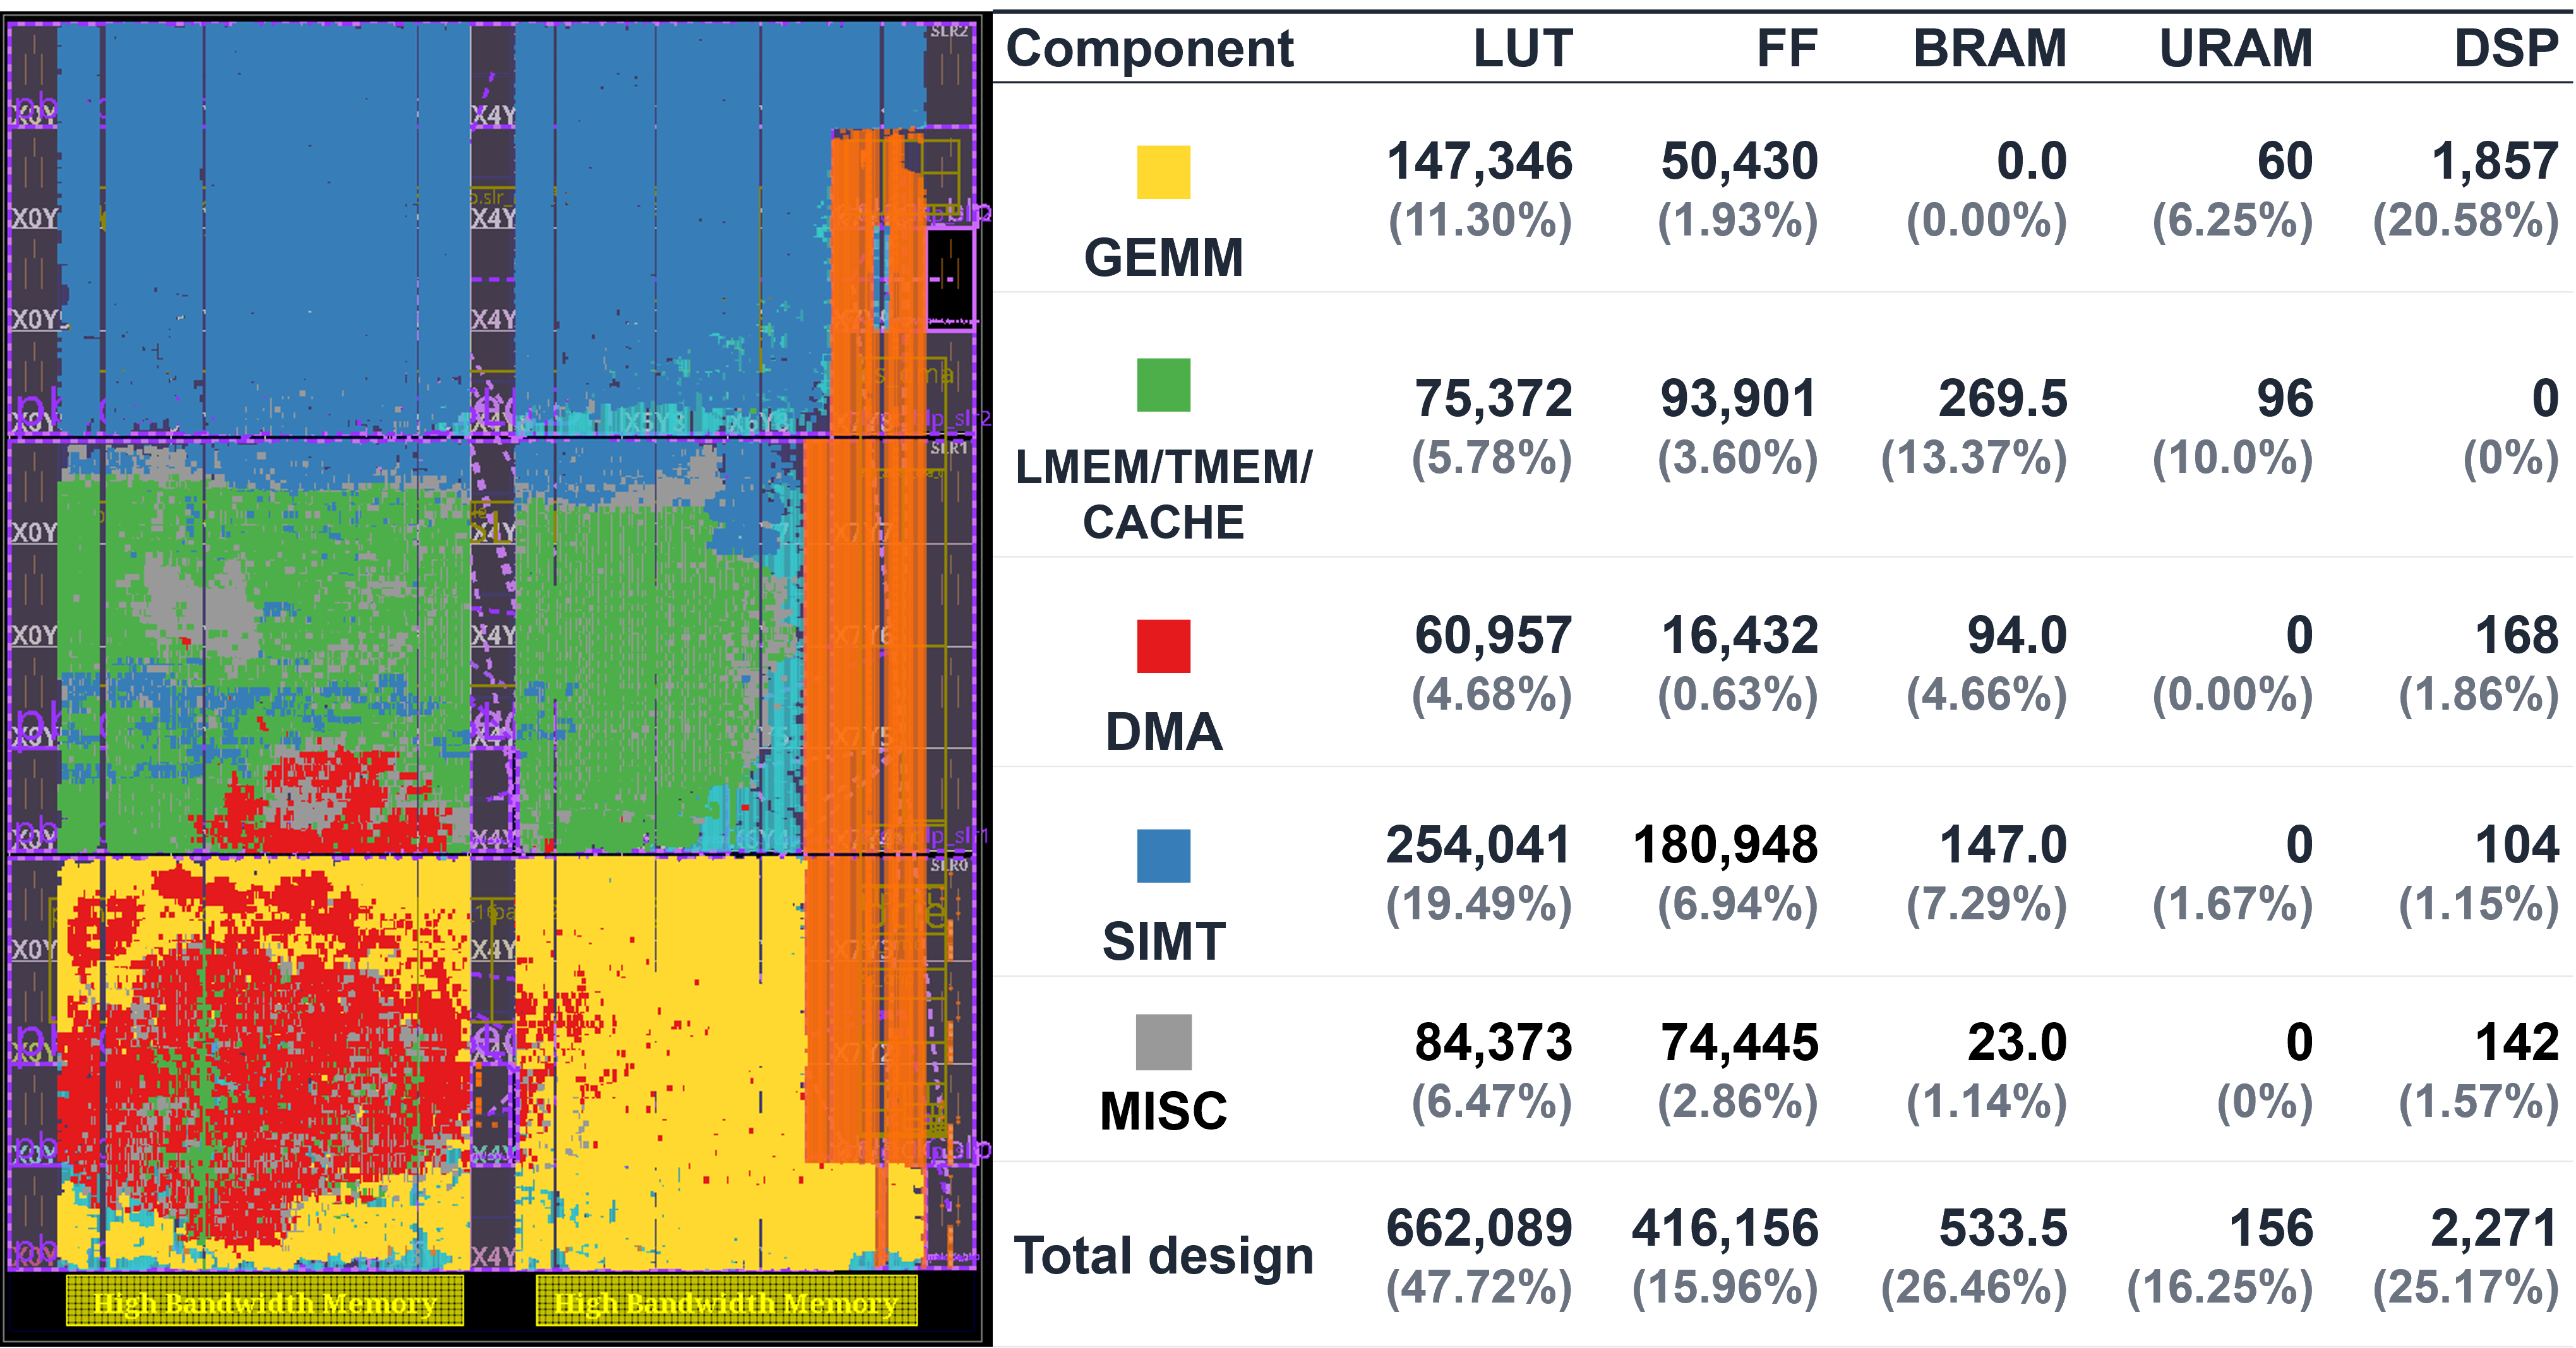
\includegraphics[width=\linewidth]{figures/floorplan.png}
    \caption{Floorplan and resource breakdown of \Cfou{} on the Alveo U55C.}
    \label{fig:floorplan}
\end{figure}

Table~\ref{tab:candidates} lists the candidate parameters. All candidates use one core with 4 warps per core and 32 threads per warp. The FP TCU is 8x4x4x2, and the \fpint{} GEMM engine is a 32x32 array. Each candidate has a 32~KiB L1 instruction cache, and a 32~KiB L1 data cache for a total cache capacity of 32~KiB. When tensor memory is present, the combined local-memory and tensor-memory capacity equals the local-memory capacity of the other candidates.

All latency results come from placed-and-routed designs deployed on a Xilinx Alveo U55C FPGA at 100MHz.
Figure~\ref{fig:floorplan} shows the floorplan and resource breakdown of the final design. 
Each candidate runs the same \wkv{} quantized model and differs only in hardware mapping. 
For area normalization, candidate designs are synthesized using Synopsys Design Compiler targeting 100 MHz in a 28 nm technology node.
%We scale each GEMM kernel's latency using the relative area of the FP TCU and/or \fpint{} GEMM engine instantiated in %its candidate.
%Only these GEMM-engine areas enter the scaling factor because all other key architectural parameters, including the numbers of cores, warps, and threads, are identical across candidates.
%We use the raw FPGA latency for vector kernels because all non-GEMM kernels execute on the common SIMT pipeline.

We sample total FPGA board power with \texttt{xrt-smi} during kernel execution and take the arithmetic mean of the collected samples.
We subtract the idle board power from this mean to obtain the kernel's dynamic power.
When a kernel runs too briefly to collect enough power samples, we wrap its body in a loop and execute multiple iterations during measurement.
We compute each kernel's energy from its dynamic power and measured latency, and obtain end-to-end latency and energy by summing the corresponding per-kernel values.
The reported energy per token is the total end-to-end energy divided by the number of processed tokens.

\begin{table}[t]
\centering
\caption{Hardware candidates for evaluation.}
\label{tab:candidates}

\scriptsize
\setlength{\tabcolsep}{1pt}

\begin{tabular*}{\columnwidth}{@{\extracolsep{\fill}}*{10}{c}@{}}
  \toprule                                                                                                                                          
  ID
  & \shortstack{Cores}
  & \shortstack{Warps}
  & \shortstack{Threads}
  & \shortstack{FP TCU}
  & \shortstack{\fpint{}\\MXU}
  & \shortstack{Cache}
  & \shortstack{LMEM}
  & \shortstack{TMEM}
  & \shortstack{ACC\\MEM} \\
  \midrule
  C1 & 1 & 4 & 32 & 8x4x4x2 & --    & 32K & 1M & -- & -- \\
  C2 & 1 & 4 & 32 & 8x4x4x2 & 32x32 & 32K & 1M & -- & -- \\
  C3 & 1 & 4 & 32 & --      & 32x32 & 32K & 1M & -- & -- \\
  C4 & 1 & 4 & 32 & --      & 32x32 & 32K & 512K & 256K & 256K \\
  \bottomrule
  \end{tabular*}
\end{table}

\textbf{Workloads.}
The evaluation covers prefill, decode, and end-to-end inference. 
The workloads are Llama2-7B and Llama3-8B, quantized with SpinQuant to 4-bit weights and KV.
We include all vector kernels used by SpinQuant, including the Hadamard transform.
GEMM operations execute on the FP TCU and/or \fpint{} GEMM engine available in each candidate.
In C4, vector kernels adjacent to GEMM operations fuse the layout
transformation to avoid a separate transformation pass.
% The quantization options follow the default parameters of SpinQuant.

\textbf{Software Implementation.}
The kernel launch code uses the Vortex runtime, and kernels are implemented natively in C++ for Vortex. 
Vector operations follow an SPMD style, while GEMM operations use either the Vortex FP TCU kernels or the \fpint{} MXU through MMIO-programmed GEMM descriptors. 
A kernel writes the matrix size, RHS transpose flag, quantization direction, and related metadata, invokes the GEMM node, and polls an MMIO status register until completion. 
Execution order, descriptor setup, and layout handling are expressed directly in the native kernels and runtime code.
We use the same sequential kernel execution model for all candidates.
The $QK^T$ GEMM completes and writes the attention score tensor to HBM before a separate Vortex SIMD kernel reads it and computes online softmax.
The softmax output is then written back to HBM and consumed by the following PV GEMM kernel.
Online softmax therefore refers to the algorithm used inside the standalone SIMD kernel.
We do not fuse $QK^T$, softmax, and PV into a single tiled attention kernel.
The reported latency and energy include these kernels and their intermediate HBM transfers.
This common execution model ensures that all candidates use the same attention schedule while differing in the GEMM datapath and memory system.
This implementation evaluates \ours{} inside an LLM inference flow rather than as a bare GEMM microbenchmark, so the memory system, runtime layout, and native \fpint{} attention support operate together.

\subsection{End-to-End Performance Improvement}

% \begin{figure}[!t]
%     \centering

%     \begin{subfigure}[t]{\linewidth}
%         \centering
%         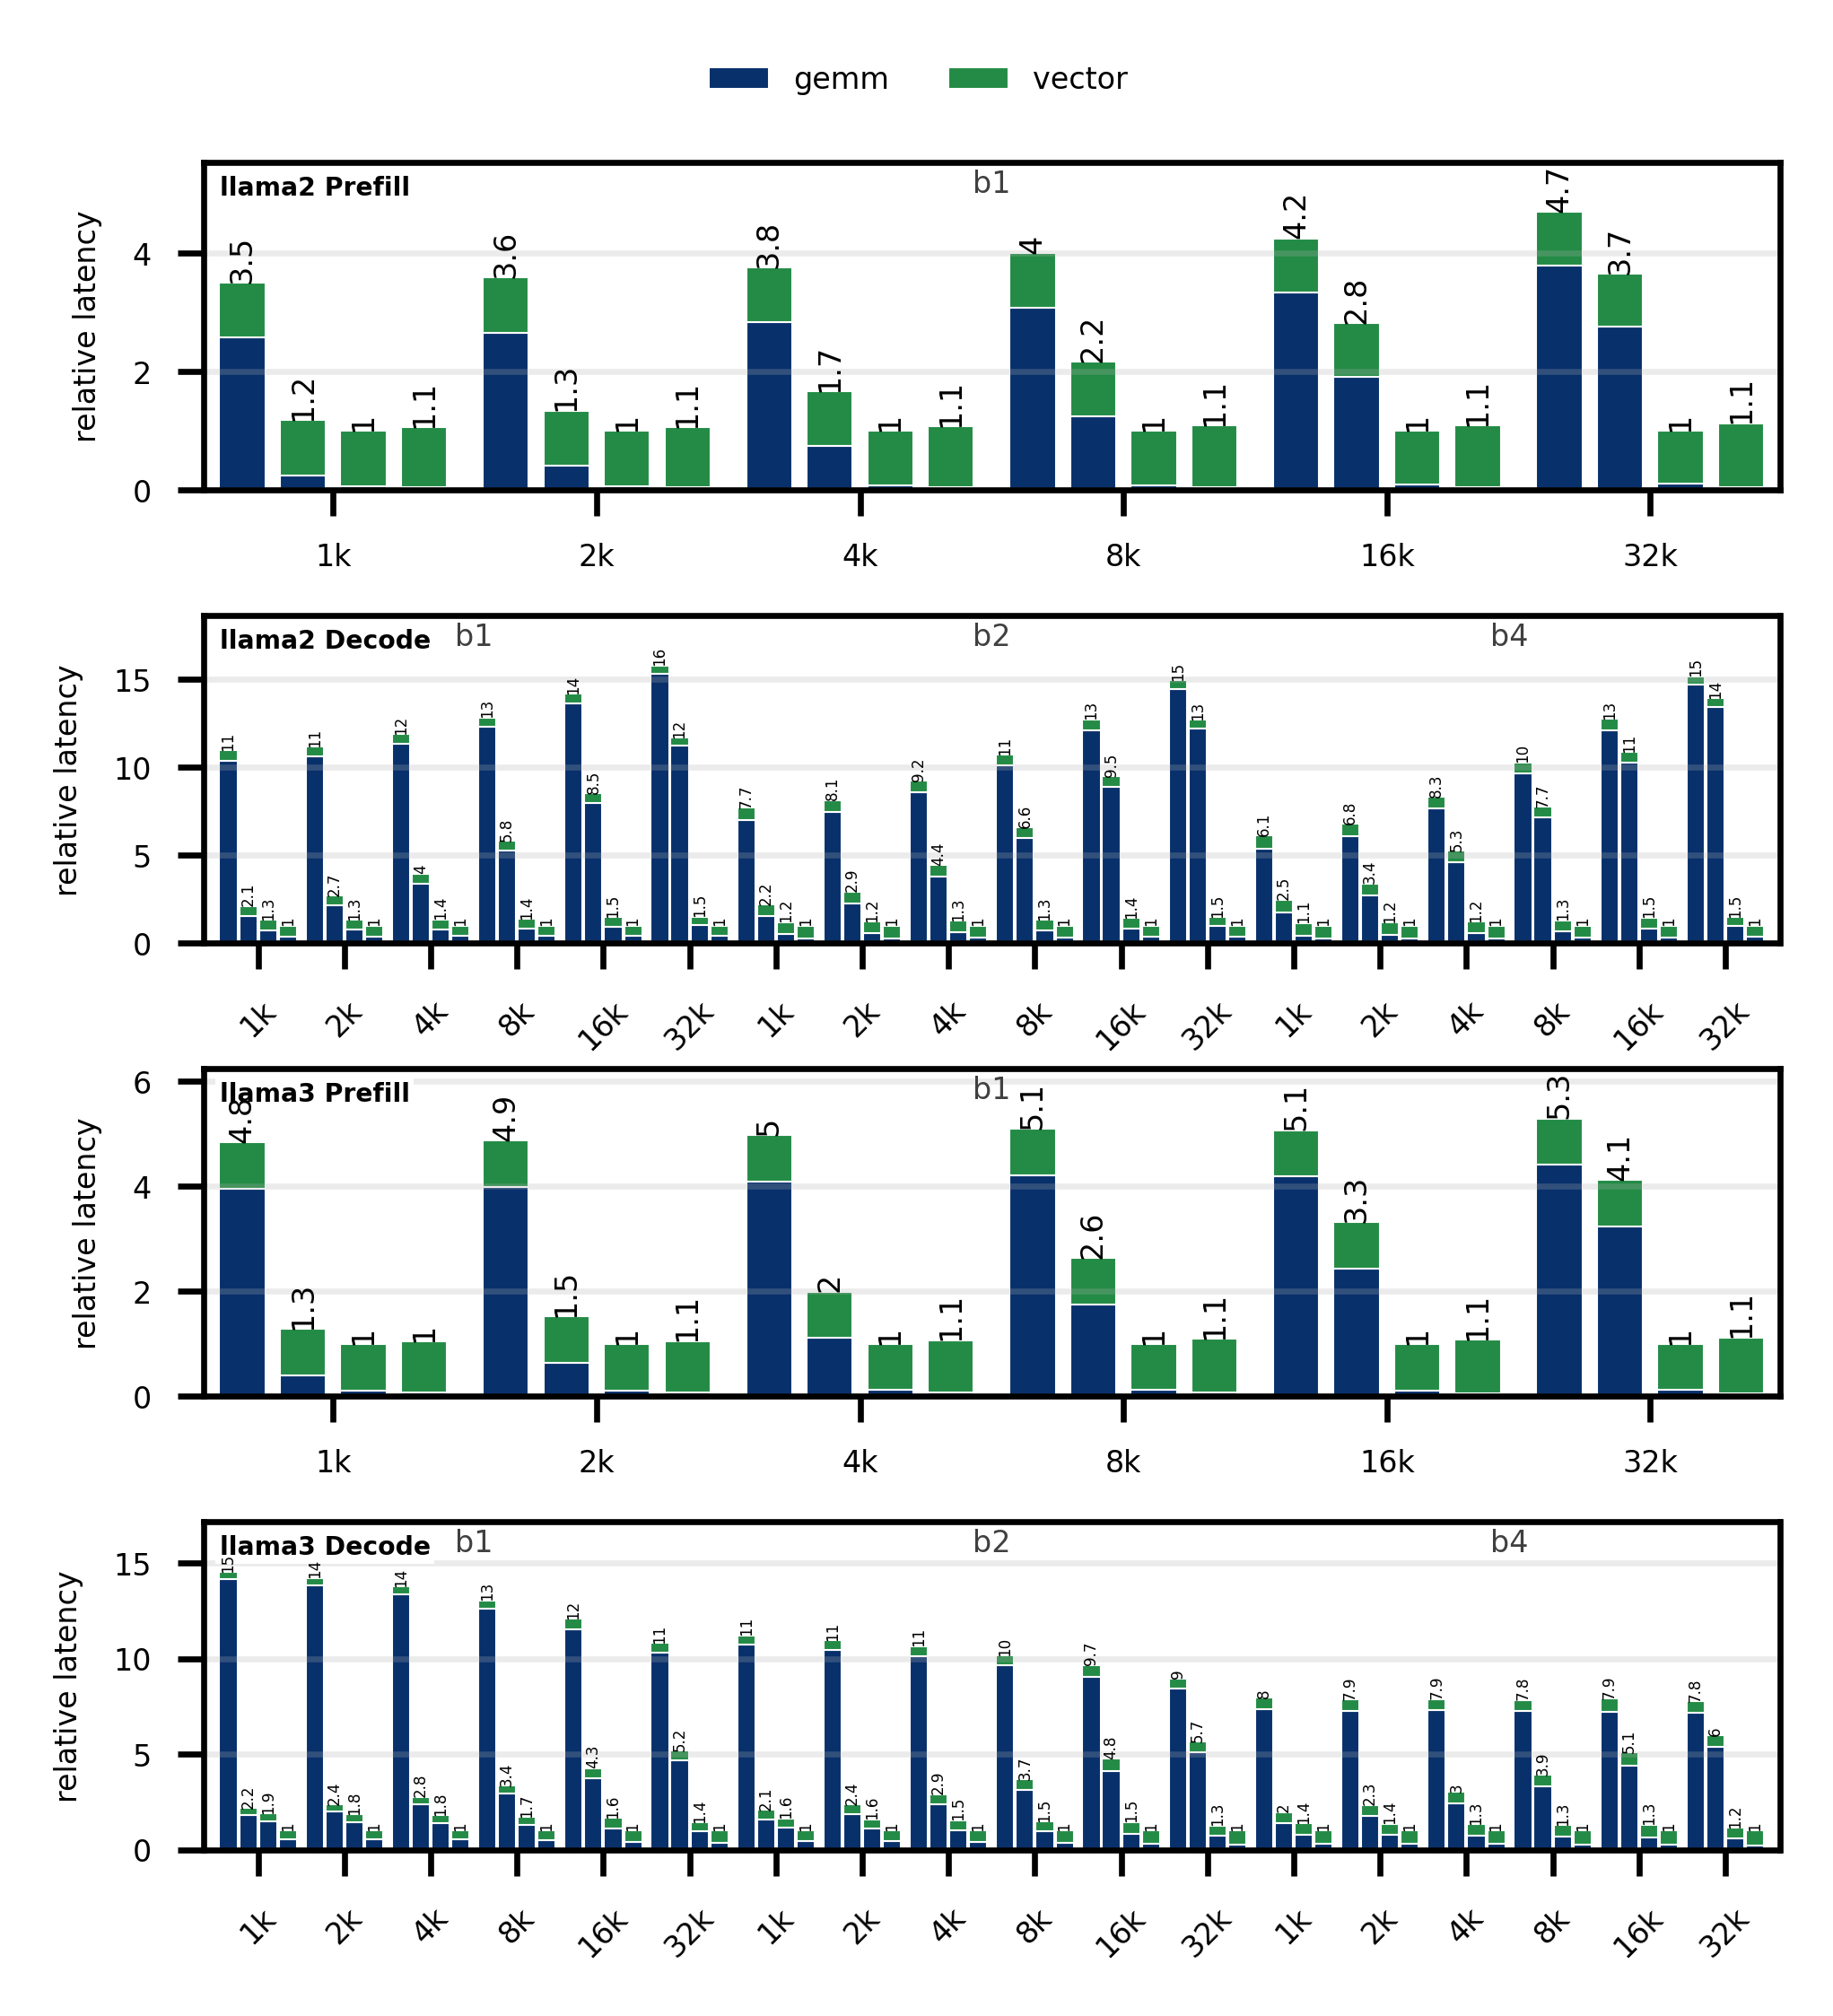
\includegraphics[width=0.92\linewidth]{figures/llama2_3/figures_script/llama_e2e_no_area_norm_stacked/llama_e2e_latency_no_area_norm_stacked.png}
%         \caption{Without area normalization.}
%         \label{fig:e2e-latency-no-area-norm}
%     \end{subfigure}

%     \vspace{0.3em}

%     \begin{subfigure}[t]{\linewidth}
%         \centering
%         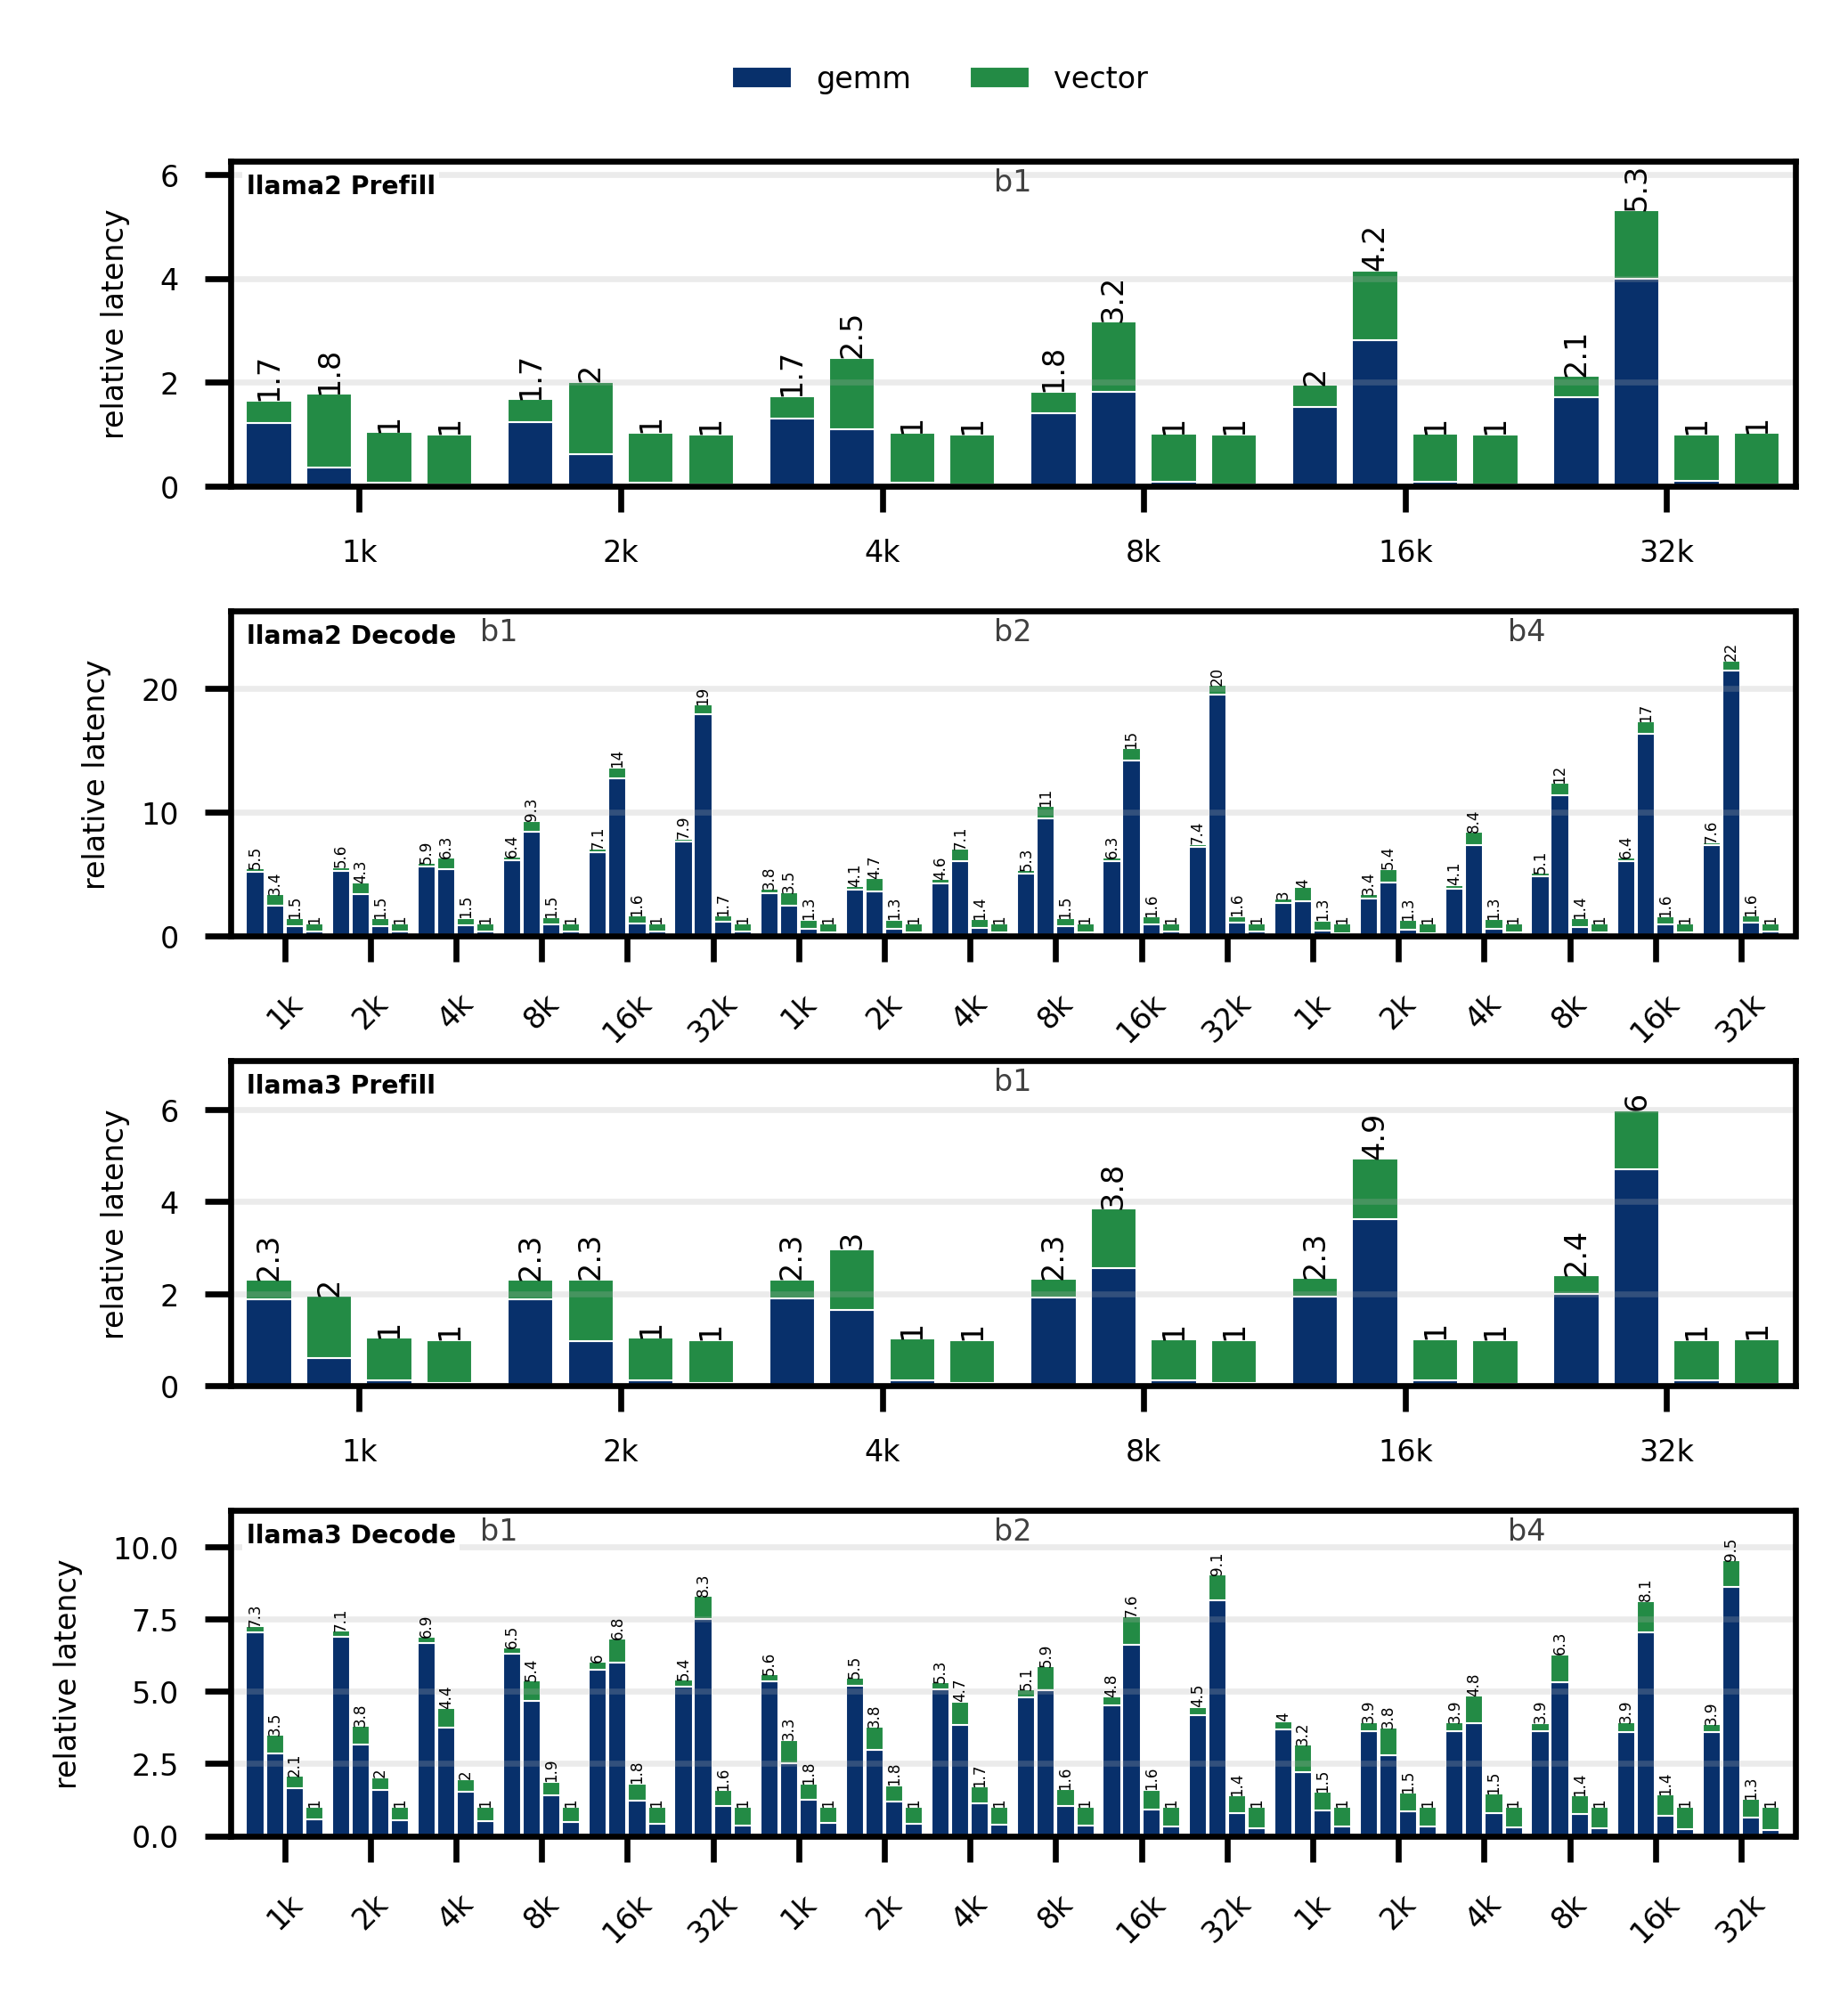
\includegraphics[width=0.92\linewidth]{figures/llama2_3/figures_script/llama_e2e_stacked/llama_e2e_latency_stacked.png}
%         \caption{With area normalization.}
%         \label{fig:e2e-latency-area-norm}
%     \end{subfigure}

%     \caption{End-to-end relative latency of Llama2-7B and Llama3-8B W4A16KV4 inference (a) without and (b) with area normalization. Within each workload, the four bars from left to right represent C1--C4 and are normalized to C4. The vector portion includes all non-GEMM kernels, including fused layout transformations.}
%     \label{fig:e2e-latency-stacked}
% \end{figure}
\begin{figure*}[!t]
    \centering

    \begin{subfigure}[t]{0.49\textwidth}
        \centering
        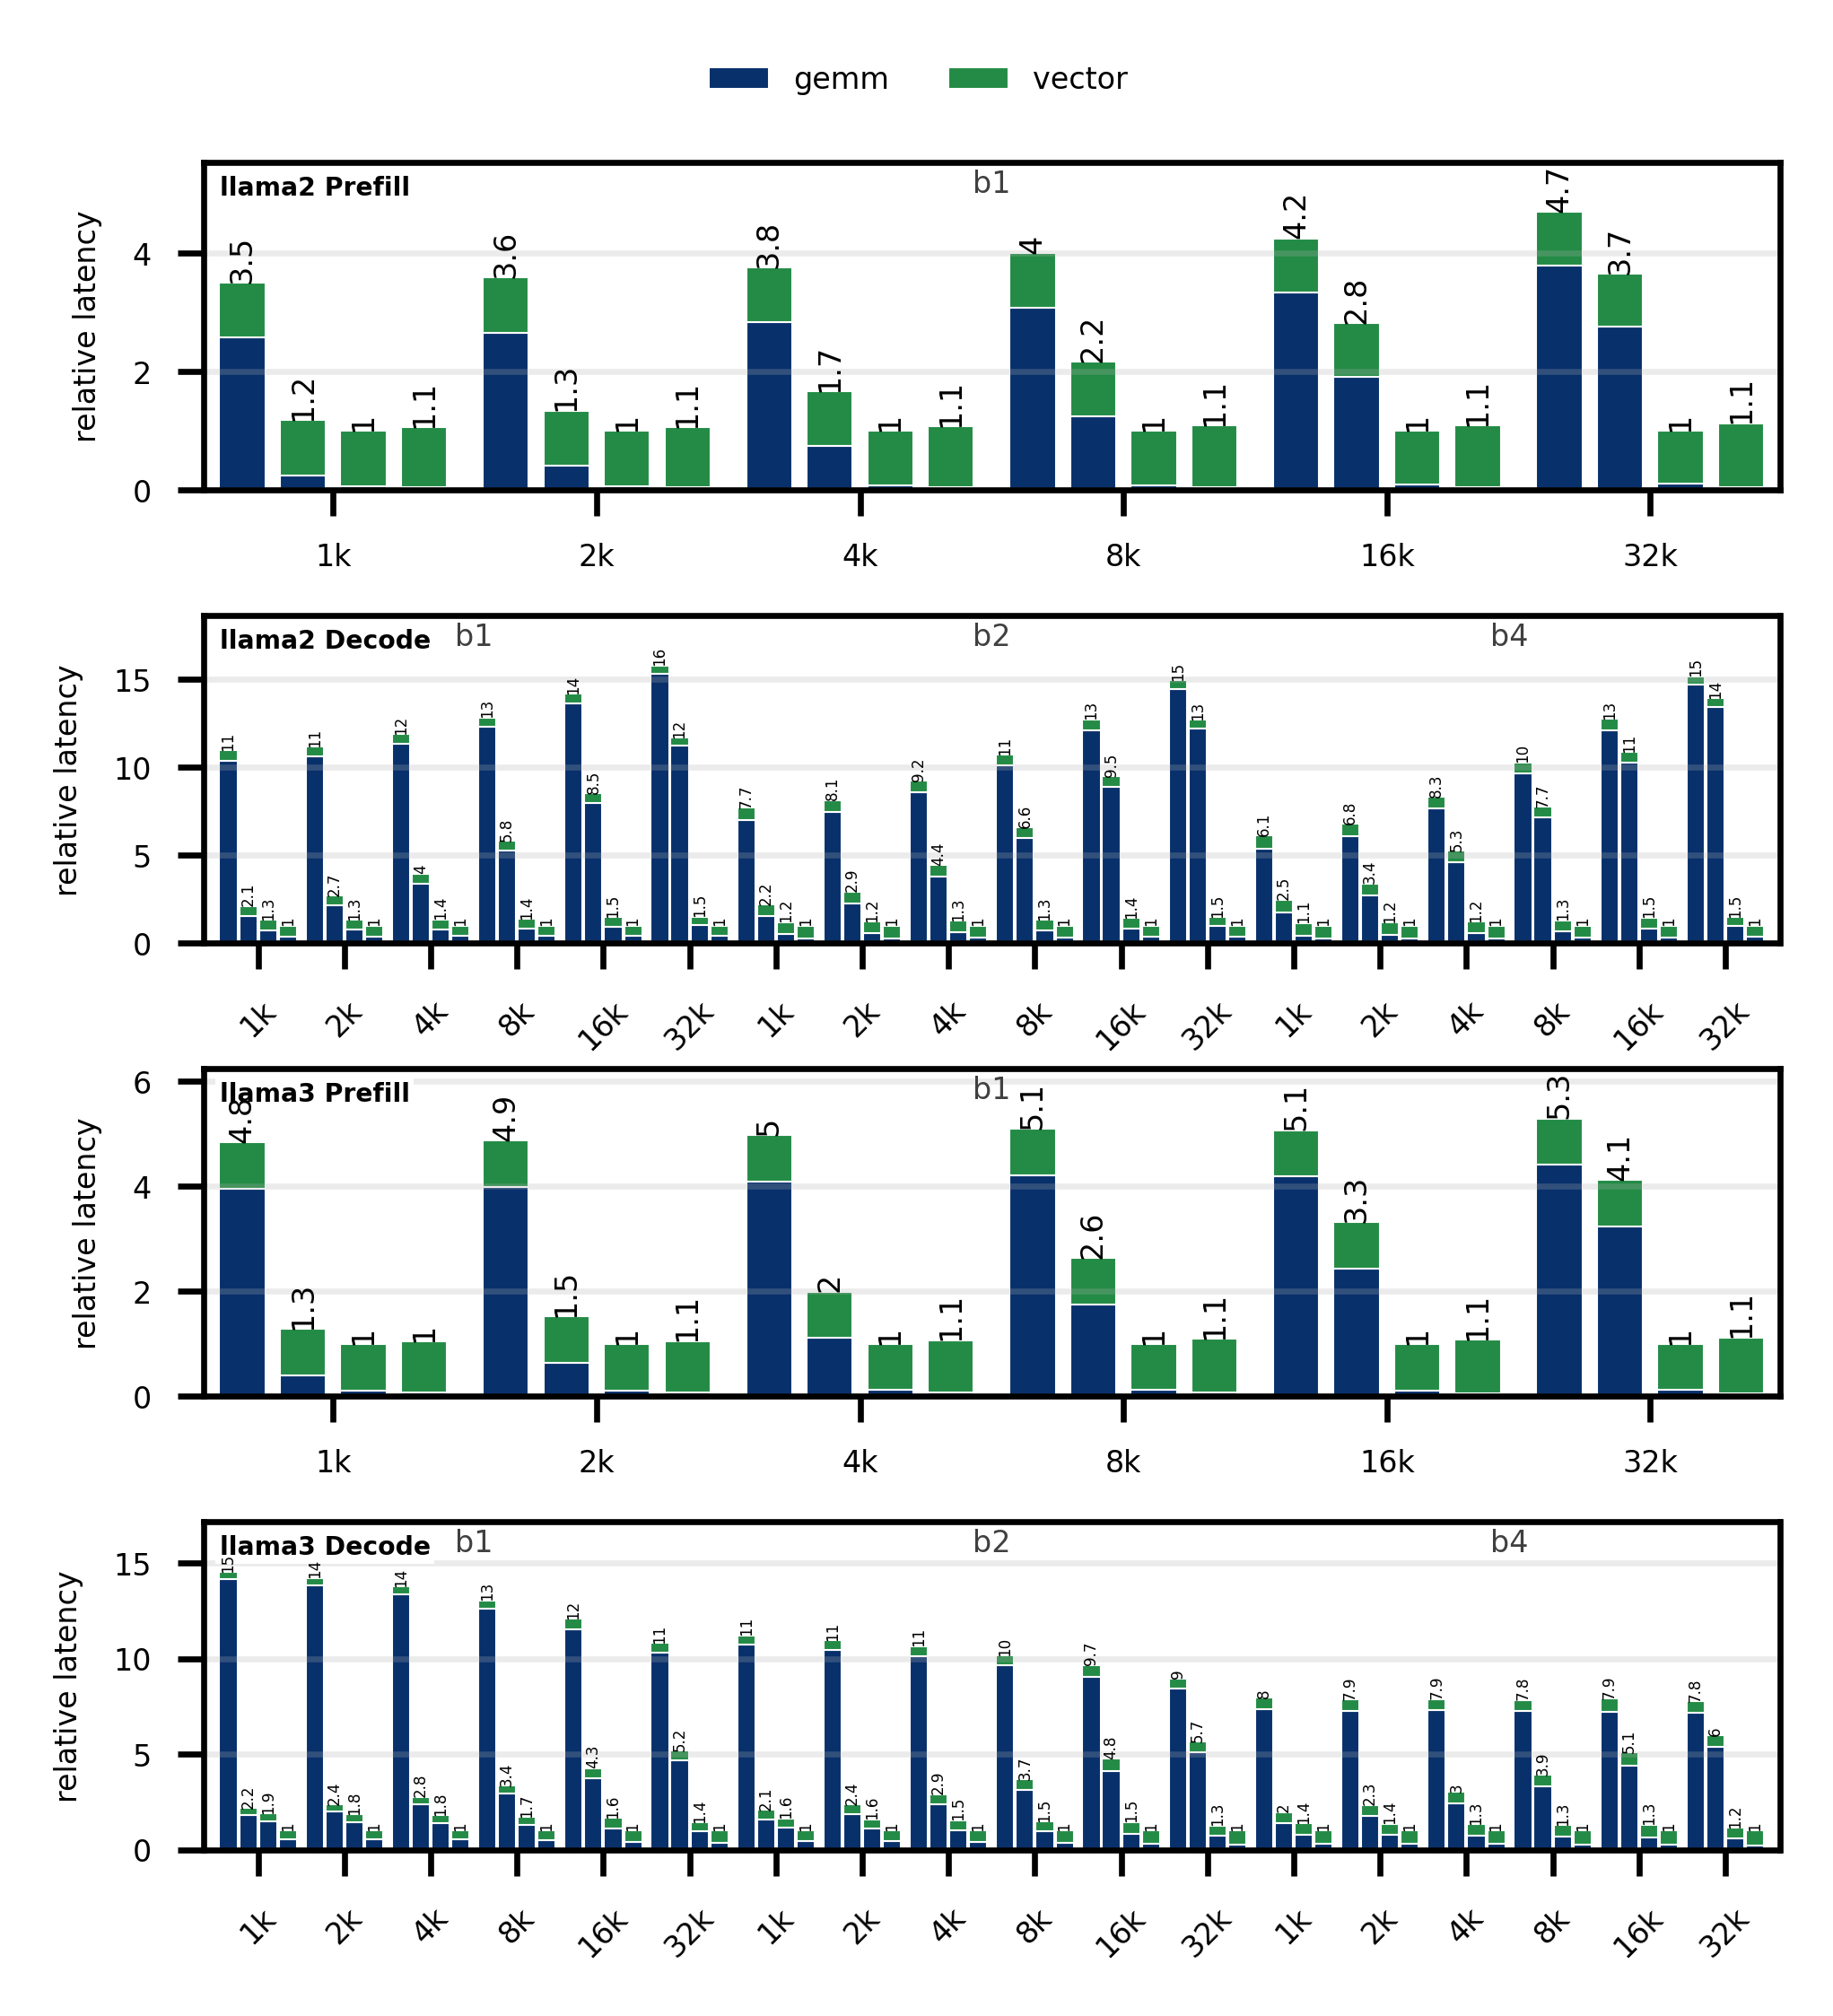
\includegraphics[width=0.92\linewidth]{figures/llama2_3/figures_script/llama_e2e_no_area_norm_stacked/llama_e2e_latency_no_area_norm_stacked.png}
        \caption{Without area normalization.}
        \label{fig:e2e-latency-no-area-norm}
    \end{subfigure}
    \hfill
    \begin{subfigure}[t]{0.49\textwidth}
        \centering
        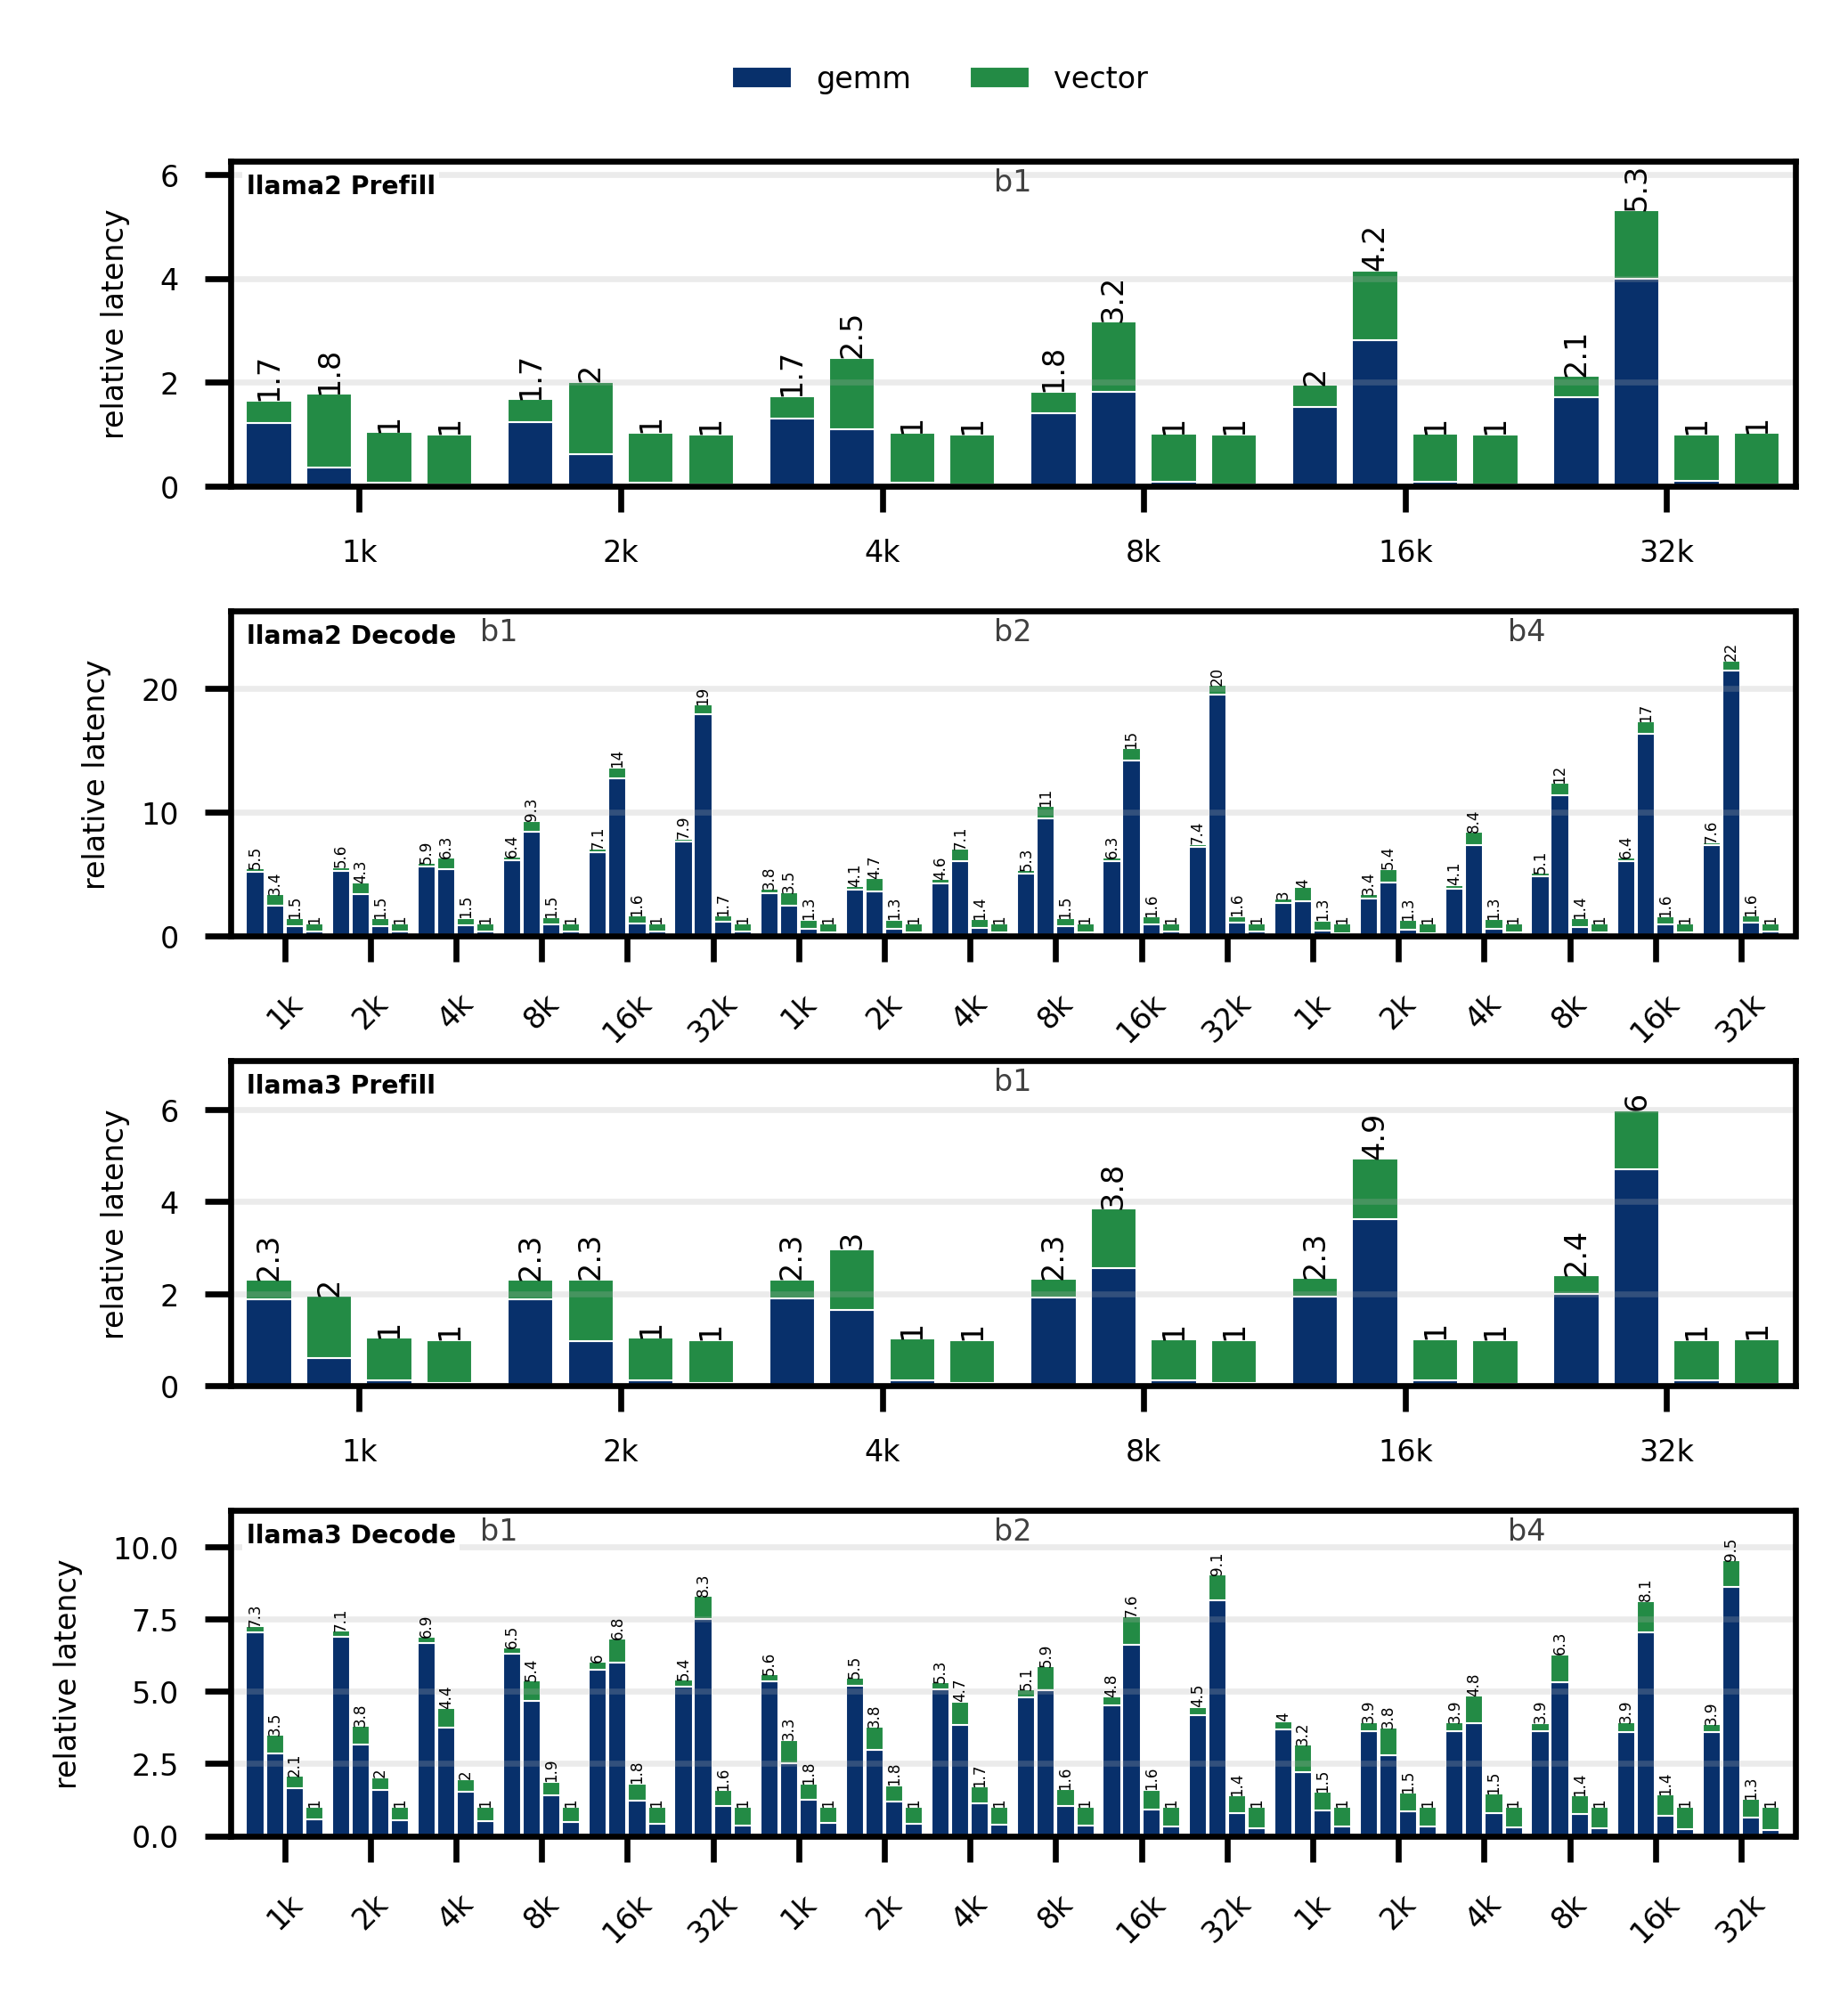
\includegraphics[width=0.92\linewidth]{figures/llama2_3/figures_script/llama_e2e_stacked/llama_e2e_latency_stacked.png}
        \caption{With area normalization.}
        \label{fig:e2e-latency-area-norm}
    \end{subfigure}

    \caption{End-to-end relative latency of Llama2-7B and Llama3-8B
    W4A16KV4 inference (a) without and (b) with area normalization.
    Within each workload, the four bars from left to right represent
    C1--C4 and are normalized to C4. The vector portion includes all
    non-GEMM kernels, including fused layout transformations.}
    \label{fig:e2e-latency-stacked}
\end{figure*}

Figure~\ref{fig:e2e-latency-stacked} compares the end-to-end latency of C1--C4 without and with area normalization when running Llama2-7B and Llama3-8B inference with 4-bit weight and KV-cache quantization.
We evaluate prefill at batch size 1 and decode at batch sizes 1, 2, and 4, with sequence lengths ranging from 1k to 32k.
In the area-normalized results in Figure~\ref{fig:e2e-latency-area-norm}, \Cfou{} reduces latency over the FP TCU baseline by $3.24\times$ on geomean in prefill
and $4.73\times$ on geomean in decode, with maximum improvements of $4.31\times$ and $7.96\times$, respectively.

Comparing C1 and C2 shows why a linear-only \fpint{} accelerator is insufficient. 
C2 accelerates the linear projections, but it still executes $QK^T$ and PV on the FP TCU while carrying the area cost of both the FP TCU and the \fpint{} MXU.
Consequently, C2's geomean latency is $1.30\times$ that of C1 in prefill and $1.94\times$ that of C1 in decode.
C2 is slower than C1 in 8 of the 12 prefill cases and in all 36 decode cases.
These results demonstrate that accelerating only the linear layers does not preserve the array-level efficiency advantage at the system level when attention remains on the FP datapath.

C3 routes both the linear layers and the $QK^T$ and PV GEMMs through the \fpint{} path, eliminating the FP attention fallback.
This change reduces geomean latency over C2 by $2.31\times$ in prefill and $2.20\times$ in decode, demonstrating the importance of supporting attention on the same \fpint{} datapath as the linear layers.

C4 further reduces geomean latency over C3 by $1.83\times$ in prefill and $4.18\times$ in decode.
The larger decode improvement shows that native \fpint{} attention is not sufficient by itself: the MXU must be paired with a memory subsystem and runtime that sustain tensor bandwidth.
The direct tensor path, tensor memory, DMA, and layout-aware runtime reduce the cost of supplying operands and moving KV-cache data, allowing the larger MXU to translate its array-level advantage into end-to-end performance.

% \begin{figure}[t]
%     \centering
%     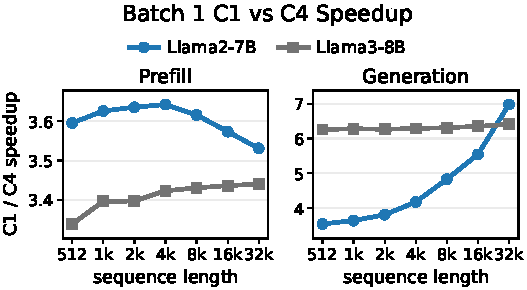
\includegraphics[width=\linewidth]{figures/llama2_3_compare/c1_vs_c4_speedup_batch1.pdf}
%     \caption{C4 speedup over C1 at batch size 1 across sequence length for Llama2-7B and Llama3-8B.}
%     \label{fig:llama3_gqa_speedup}
% \end{figure}

% To compare this trend across model architectures, Figure~\ref{fig:llama3_gqa_speedup} compares the C4-over-C1 speedup for Llama2-7B and Llama3-8B while sweeping context length.
% In prefill, the two models follow a similar trend because the prompt is processed as a full sequence and the dominant work is shared by the common hidden width, 
% query-head count, and head dimension.
% Although Llama3-8B uses GQA, reducing the number of KV heads does not change the fact that long-context prefill is dominated by full-sequence attention and softmax, 
% so its trend remains close to Llama2-7B.

% Generation exposes a different balance.
% The projection and FFN stack operates on one token per layer, so much of the C1 baseline is skinny GEMM/GEMV-shaped work that underutilizes the conventional FP tensor path.
% C4 benefits from keeping this fixed per-token work on the native \fpint{} GEMM engine and optimized tensor-memory path, and this effect is more visible 
% in Llama3-8B because its FFN is wider.
% GQA also changes the attention geometry during generation.
% Multiple query heads share one K/V head, allowing $QK^\top$ and $PV$ to concatenate those query heads along the GEMM $M$ dimension instead of issuing 
% separate GEMV-shaped operations.
% This gives C4 better utilization on Llama3-8B generation attention.
% At the same time, the smaller number of KV heads also reduces the C1 baseline attention, KV-cache quantization, layout, and movement work.
% As a result, Llama3-8B shows a high but relatively flat generation benefit, while Llama2-7B gains more with context length because its C1 
% attention path grows more directly with the KV-cache length.

The vector portion includes softmax, quantization, normalization, elementwise operations, and layout transformations fused into adjacent kernels.
Thus, the C4 results include the cost of layout handling without introducing a standalone transformation pass.
As the optimized \fpint{} path substantially reduces both linear and attention GEMM latency, these vector kernels account for a larger portion of the remaining end-to-end latency, particularly during prefill.
This result shows that the performance bottleneck shifts toward vector processing after GEMM acceleration.

\subsection{GEMM Latency Breakdown}

Figure~\ref{fig:gemm-breakdown} decomposes area-normalized GEMM latency into the Q/K/V/O projections, the $QK^T$ and PV attention GEMMs, and the FFN projections.
This breakdown isolates which architectural step produces the end-to-end speedup in Figure~\ref{fig:e2e-latency-stacked}.
Compared with C1, C4 reduces total GEMM latency by $36.60\times$ on geomean in prefill and $13.42\times$ on geomean in decode.

Comparing C1 and C2 exposes the limitation of accelerating only the linear layers.
In prefill, C2 reduces the Q/K/V/O and FFN projection latency over C1 by $1.40\times$ and $1.54\times$, respectively.
However, C2 leaves $QK^T$ and PV on the FP TCU while carrying the area cost of both the FP TCU and the \fpint{} MXU.
Under area normalization, its attention GEMM latency is therefore $3.51\times$ that of C1 in both prefill and decode.
The area cost also offsets the linear-layer gains for the skinny GEMMs in decode.
Consequently, C2's total GEMM latency is $1.40\times$ that of C1 in prefill and $1.99\times$ that of C1 in decode.

C3 routes the attention GEMMs through the \fpint{} path and removes the FP attention fallback.
This change reduces attention GEMM latency over C2 by $11.24\times$ in prefill and $4.92\times$ in decode, yielding total GEMM improvements of $3.24\times$ and $2.28\times$, respectively.
The benefit becomes critical at long contexts: at a sequence length of 32k, attention accounts for an average of 91.7\% of C2's GEMM latency in prefill and 81.5\% in decode across the evaluated models and batches.

C3 and C4 execute both linear and attention GEMMs on the same \fpint{} arithmetic path, so their difference isolates the system that feeds the MXU.
C4 reduces total GEMM latency over C3 by $15.83\times$ in prefill and $11.75\times$ in decode.
The improvement spans the linear and attention groups, showing that the direct tensor path, tensor memory, DMA, and layout/runtime support sustain the larger array across GEMM types.
Although these GEMM-only improvements are much larger than the corresponding end-to-end gains, the optimized GEMM path shifts the remaining execution time toward vector kernels, as shown in Figure~\ref{fig:e2e-latency-stacked}.

\begin{figure}[t]
    \centering
    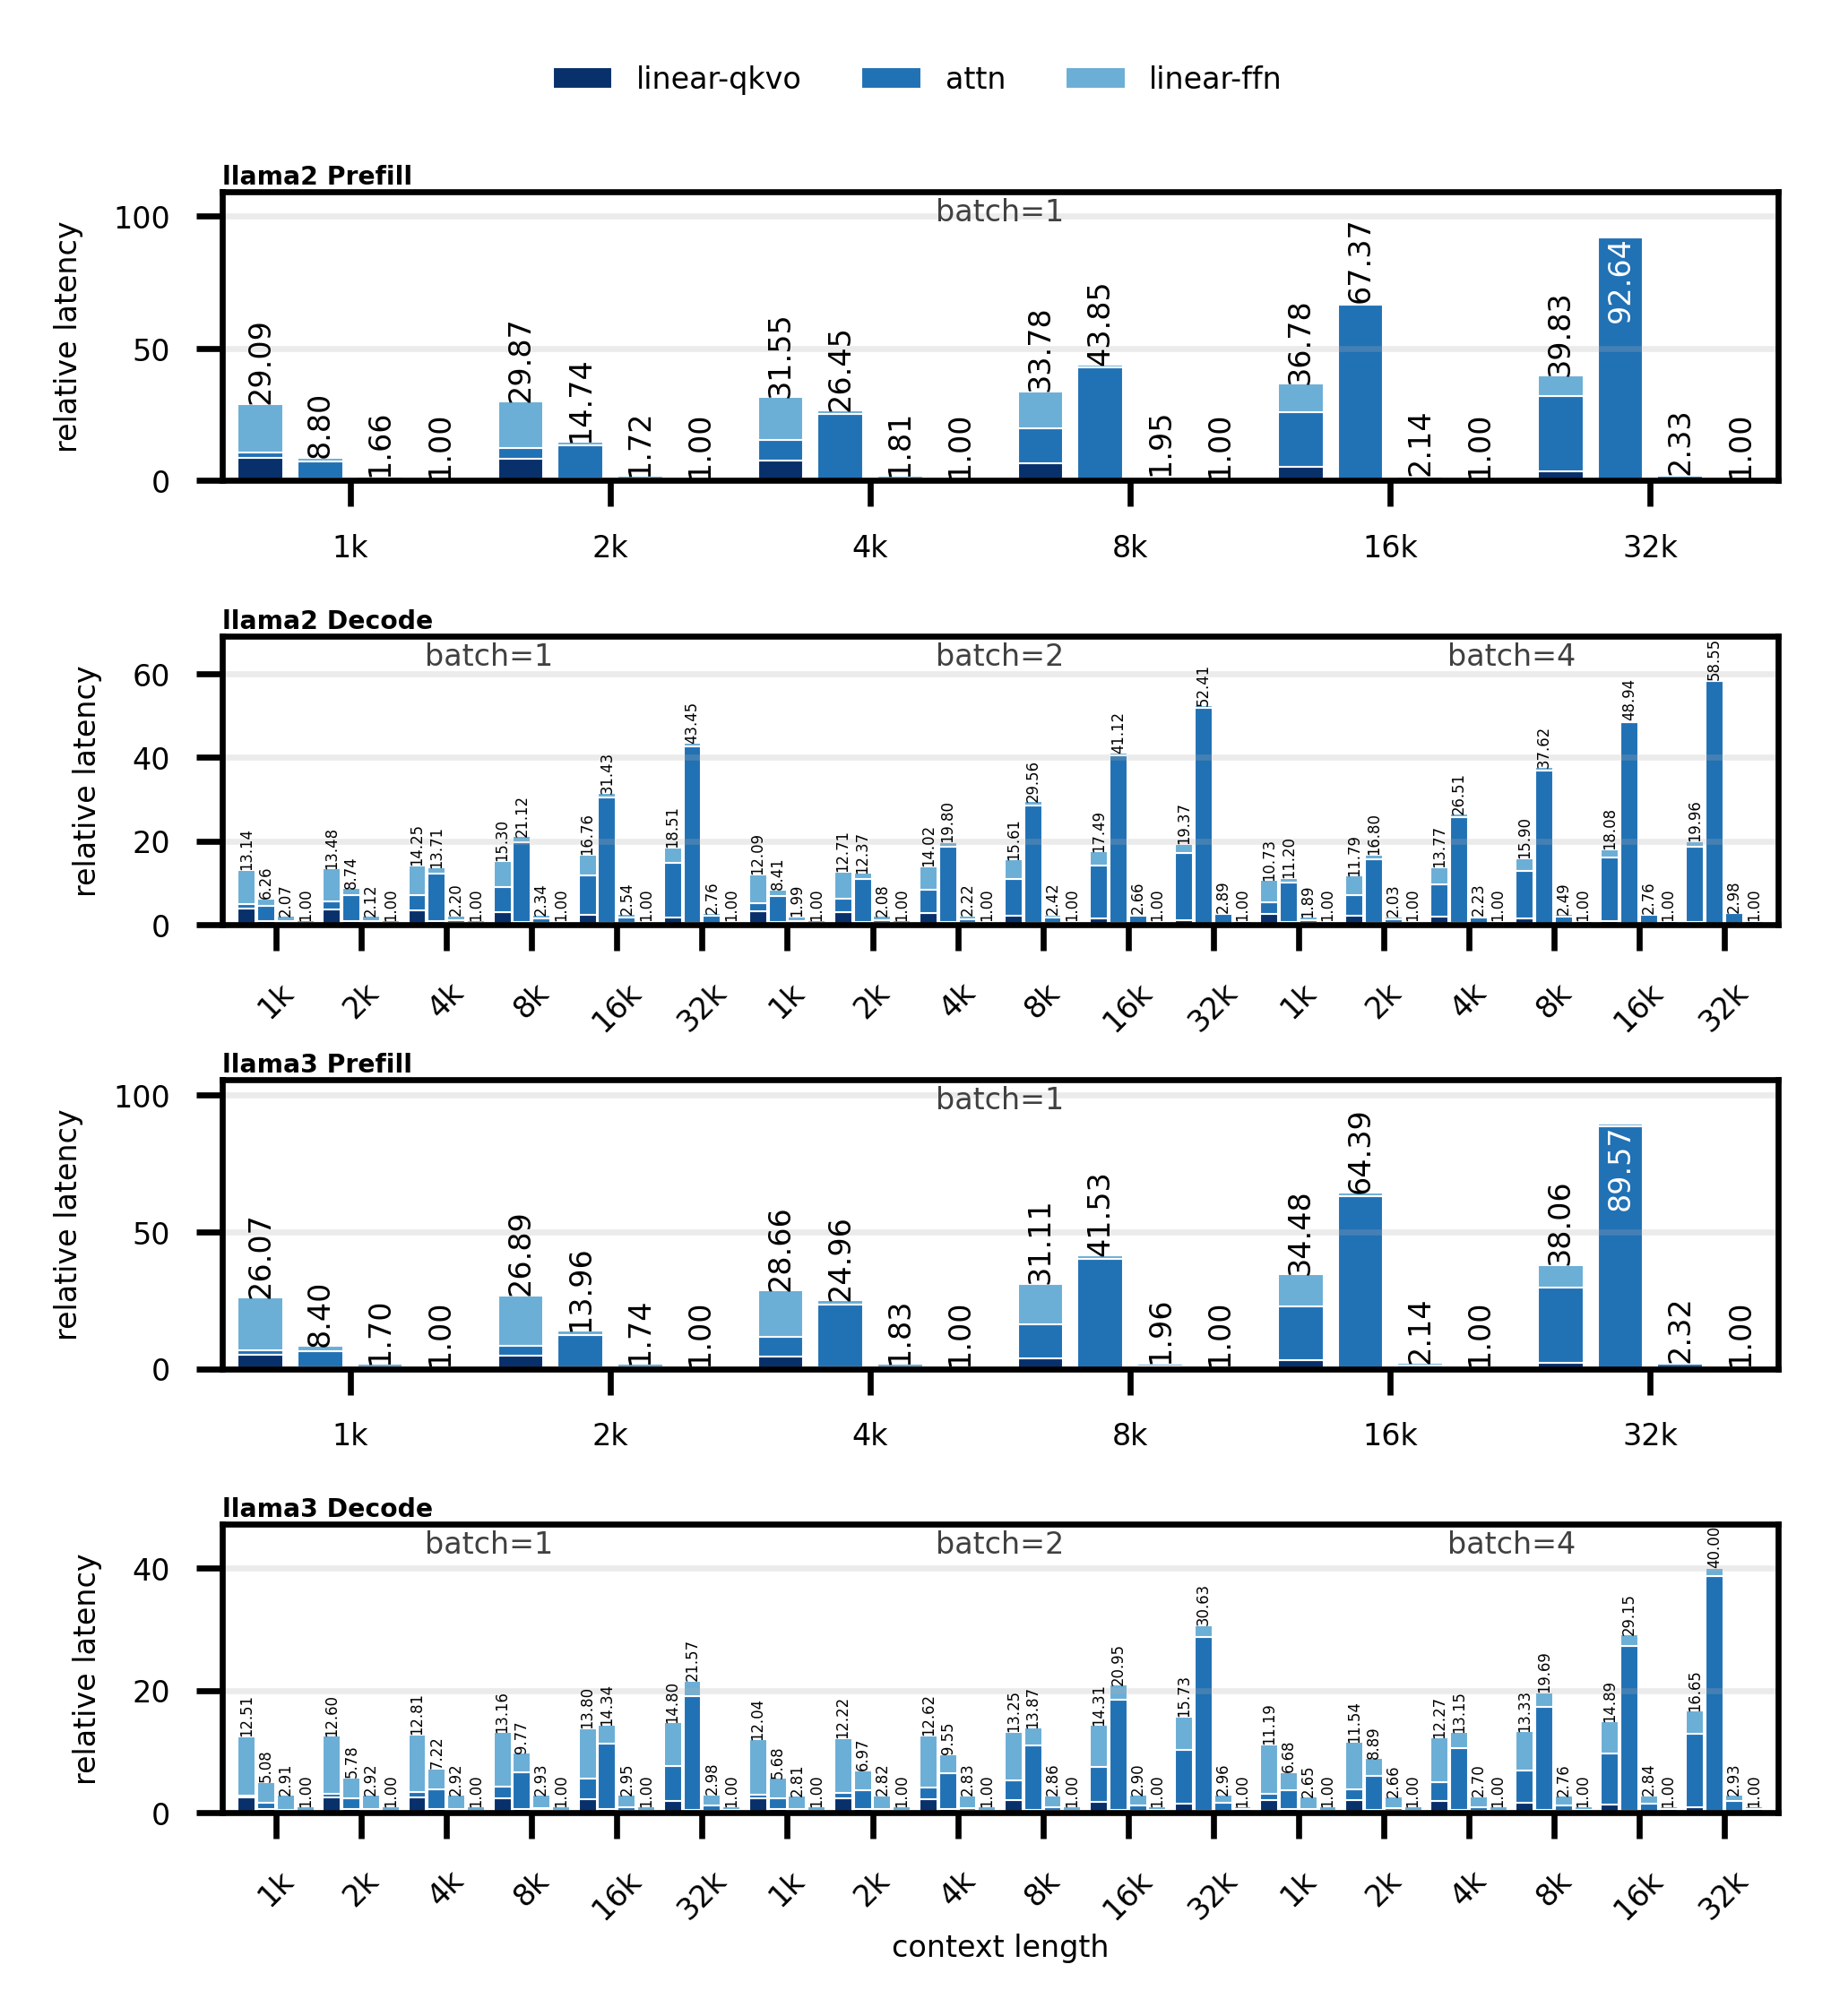
\includegraphics[width=\columnwidth]{figures/llama2_3/figures_script/llama_gemm_only/llama_gemm_only_latency.png}
    \caption{Area-normalized GEMM latency breakdown for linear projections and attention. Within each workload, the four stacked bars from left to right represent C1--C4 and are normalized to C4. Colors group the Q/K/V/O projections, attention GEMMs, and FFN projections.}
    \label{fig:gemm-breakdown}
\end{figure}

\subsection{End-to-End Energy Efficiency}

\begin{figure}[t]
    \centering
    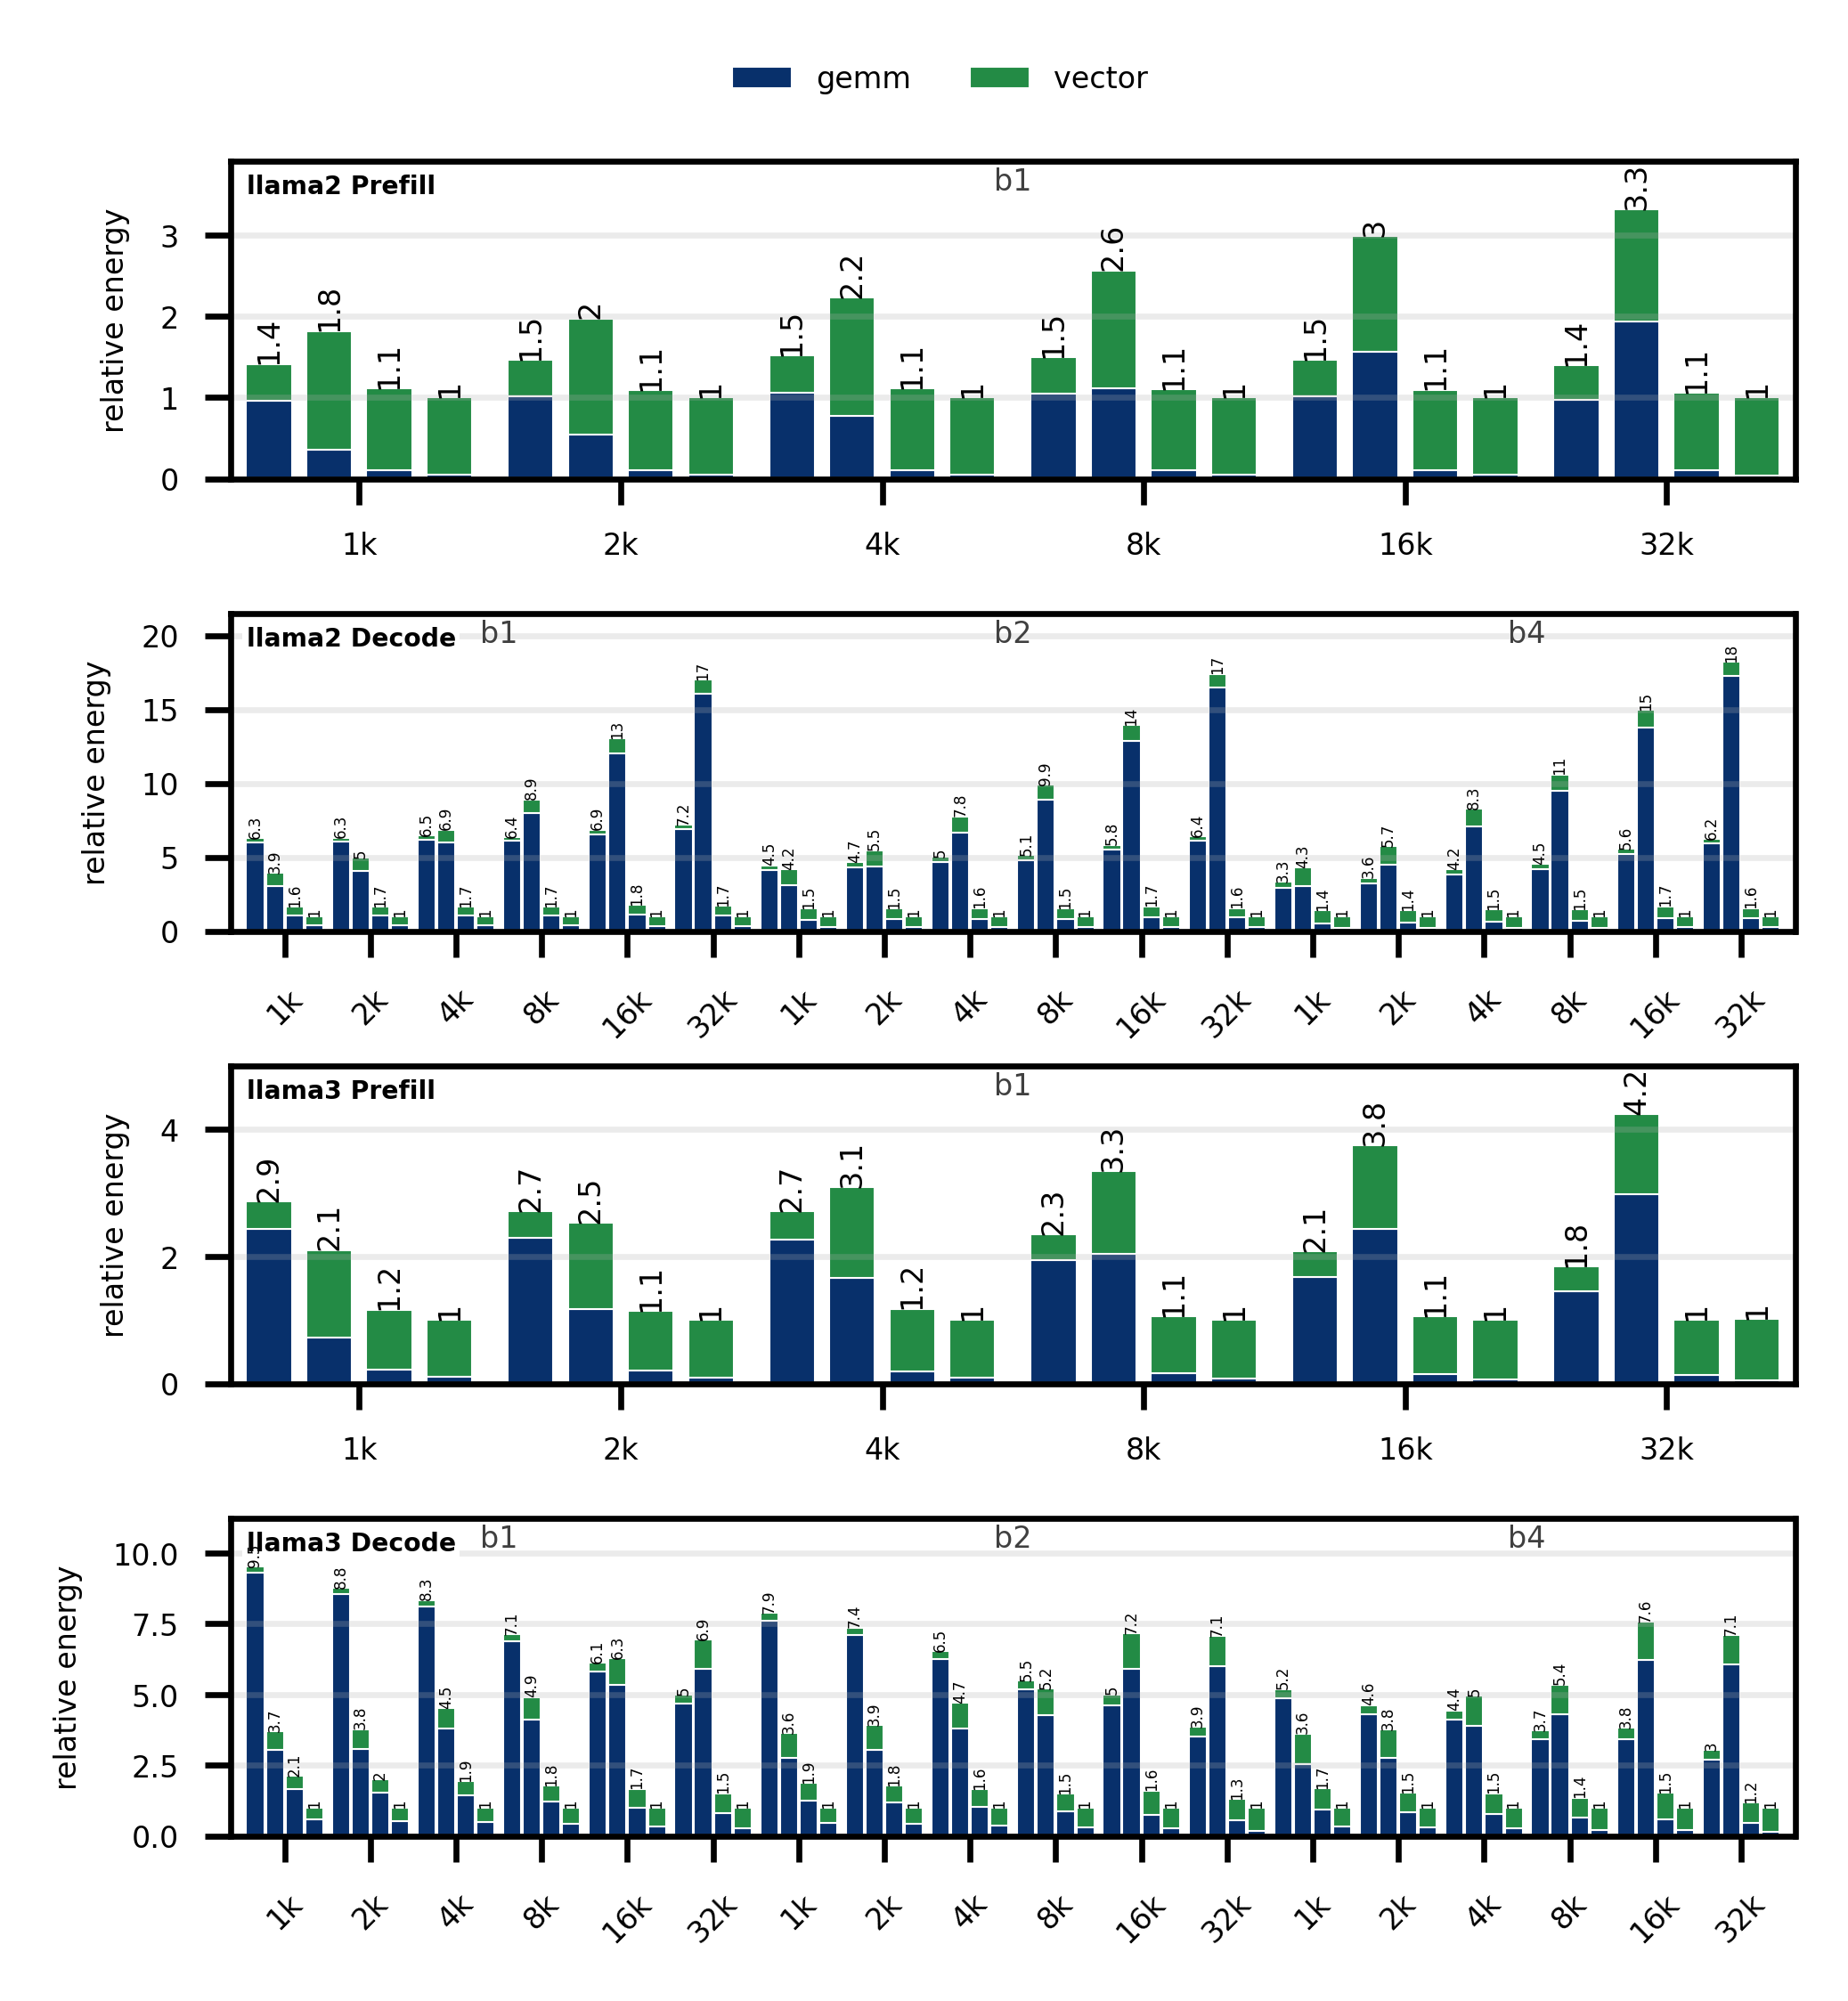
\includegraphics[width=\columnwidth]{figures/llama2_3/figures_script/llama_energy_stacked/llama_energy_per_token_power_dynamic_avg_W_stacked.png}
    \caption{End-to-end energy per token with idle power subtracted. Within each workload, the four bars from left to right represent C1--C4 and are normalized to C4. The vector portion includes all non-GEMM kernels, including fused layout transformations.}
    \label{fig:energy_per_token}
\end{figure}

Figure~\ref{fig:energy_per_token} reports end-to-end energy per token after subtracting idle board power. 
\Cfou{} reduces energy per token over C1 by $4.75\times$ on geomean in prefill and $7.93\times$ on geomean in decode.
The energy results broadly follow the latency trend.

C2 provides only a mixed energy benefit, reducing geomean energy over C1 by $1.07\times$ in prefill, whereas its decode energy is $1.19\times$ that of C1.
C3 reduces energy over C2 by $3.13\times$ in prefill and $3.46\times$ in decode, and C4 further reduces it over C3 by $1.42\times$ and $2.72\times$, respectively.
Thus, the same progression from native \fpint{} attention to the optimized memory and runtime system improves both latency and energy.

At the component level, C4 reduces GEMM energy over C1 by $37.24\times$ in prefill and $20.79\times$ in decode.
After this reduction, vector kernels account for an average of 88.4\% of C4's remaining energy in prefill and 61.4\% in decode.
The energy bottleneck therefore shifts toward vector processing, particularly during prefill.

\subsection{Accuracy}

\begin{table*}[t]
\centering
\caption{Zero-shot accuracy (\%) on eight downstream tasks and WikiText-2 perplexity (PPL) for Llama2-7B W4A16KV4 variants.}
\label{tab:accuracy}

\scriptsize
\setlength{\tabcolsep}{1.5pt}
\begin{tabularx}{\textwidth}{@{}>{\raggedright\arraybackslash}p{0.18\textwidth}YYYYYYYYY|Y@{}}
\toprule
& ARC-c & ARC-e & BoolQ & HellaSwag & OBQA & PIQA & SocialQA & WinoG & Avg. $\uparrow$ & PPL $\downarrow$ \\
\midrule
W4A16KV4 & 44.20 & 73.15 & 76.85 & 75.35 & 42.60 & 78.56 & 45.24 & 68.82 & 63.10 & 5.59 \\
W4A16KV4 (linear) & 44.37 & 72.98 & 76.24 & 75.34 & 43.20 & 78.40 & 45.29 & 69.22 & 63.13 & 5.59 \\
W4A16KV4 (attn) & 44.03 & 73.32 & 76.82 & 75.23 & 43.20 & 78.56 & 44.73 & 68.19 & 63.01 & 5.59 \\
\rowcolor{gray!12}
W4A16KV4 (linear and attn)
& 44.03 & 73.02 & 77.13 & 75.22 & 44.20 & 78.78 & 45.24 & 69.53 & 63.39 & 5.59\\
\bottomrule
\end{tabularx}
\end{table*}

This experiment evaluates whether executing an already quantized model on the native \fpint{} datapath changes its accuracy relative to GPU execution.
Table~\ref{tab:accuracy} compares Llama2-7B with SpinQuant W4A16KV4 using the GPU reference and native \fpint{} execution for linear layers, attention, or both.
Across the eight zero-shot tasks, the GPU reference and the proposed hardware achieve average accuracies of 63.10 and 63.39, respectively, a difference of only 0.29 percentage points; both also achieve the same WikiText-2 perplexity of 5.59.
The intermediate configurations remain within the same narrow range, showing that executing both linear layers and attention on the proposed hardware introduces no measurable accuracy degradation at the reported precision.

\subsection{Hardware Efficiency and Area Overhead}

\paragraph{Array-level efficiency and attention-support overhead}
Table~\ref{tab:array-level} shows that the WKV \fpint{} GEMM engine improves TOPS/mm$^2$ by $2.21\times$ and TOPS/W by $2.97\times$ over the FP TCU.
Compared with the weight-only GEMM engine, supporting native KV-attention GEMMs reduces these efficiencies by only 4.4\% and 2.6\%, respectively.
As shown in Figure~\ref{fig:arr-level-break}, the additional \qrow{} input scaler accounts for only 2.84\% of the WKV GEMM engine area and 0.74\% of its power.
This low overhead results from sharing 16 FP multipliers across the GEMM engine columns instead of placing 1024 multipliers across the PEs.

\begin{table}[t]
\centering
\caption{Array-level efficiency at 28\,nm and 100\,MHz for a 32$\times$32 array, normalized to the FP TCU.}
\label{tab:array-level}
\small
\setlength{\tabcolsep}{3pt}
\begin{tabularx}{\columnwidth}{@{}>{\raggedright\arraybackslash}Xccc@{}}
\toprule
Unit & Precision & TOPS/mm$^2$ & TOPS/W \\
\midrule
FP TCU & FP$\times$FP & 1.0 & 1.0 \\
WoQ \fpint{} GEMM Engine & \fpint{} & 2.32 & 3.04 \\
WKV \fpint{} GEMM Engine & \fpint{} & 2.21 & 2.97 \\
\bottomrule
\end{tabularx}
\end{table}

\begin{figure}[t]
    \centering
    \includegraphics[width=\linewidth]{figures/gemm_engine_breakdown/fig9_wkv_vs_woq_breakdown.png}
    \caption{Power and area breakdown of the weight-only (WoQ) and WKV \fpint{} GEMM engine.}
    \label{fig:arr-level-break}
\end{figure}

\paragraph{System-level area overhead}
Figure~\ref{fig:area-breakdown} shows that the GEMM engine and on-chip memories account for 40.4\% and 44.7\% of the total area, respectively, while the SIMT pipeline, including the DMA node, accounts for 11.4\%.
In contrast, the remaining DMA logic occupies 1.6\%, and miscellaneous logic including the interconnect and mux/demux occupies 1.9\%.
Their combined 3.5\% area overhead shows that the direct-connected tensor path preserves the array-level density advantage at the full-system level.

\begin{figure}[t]
    \centering
    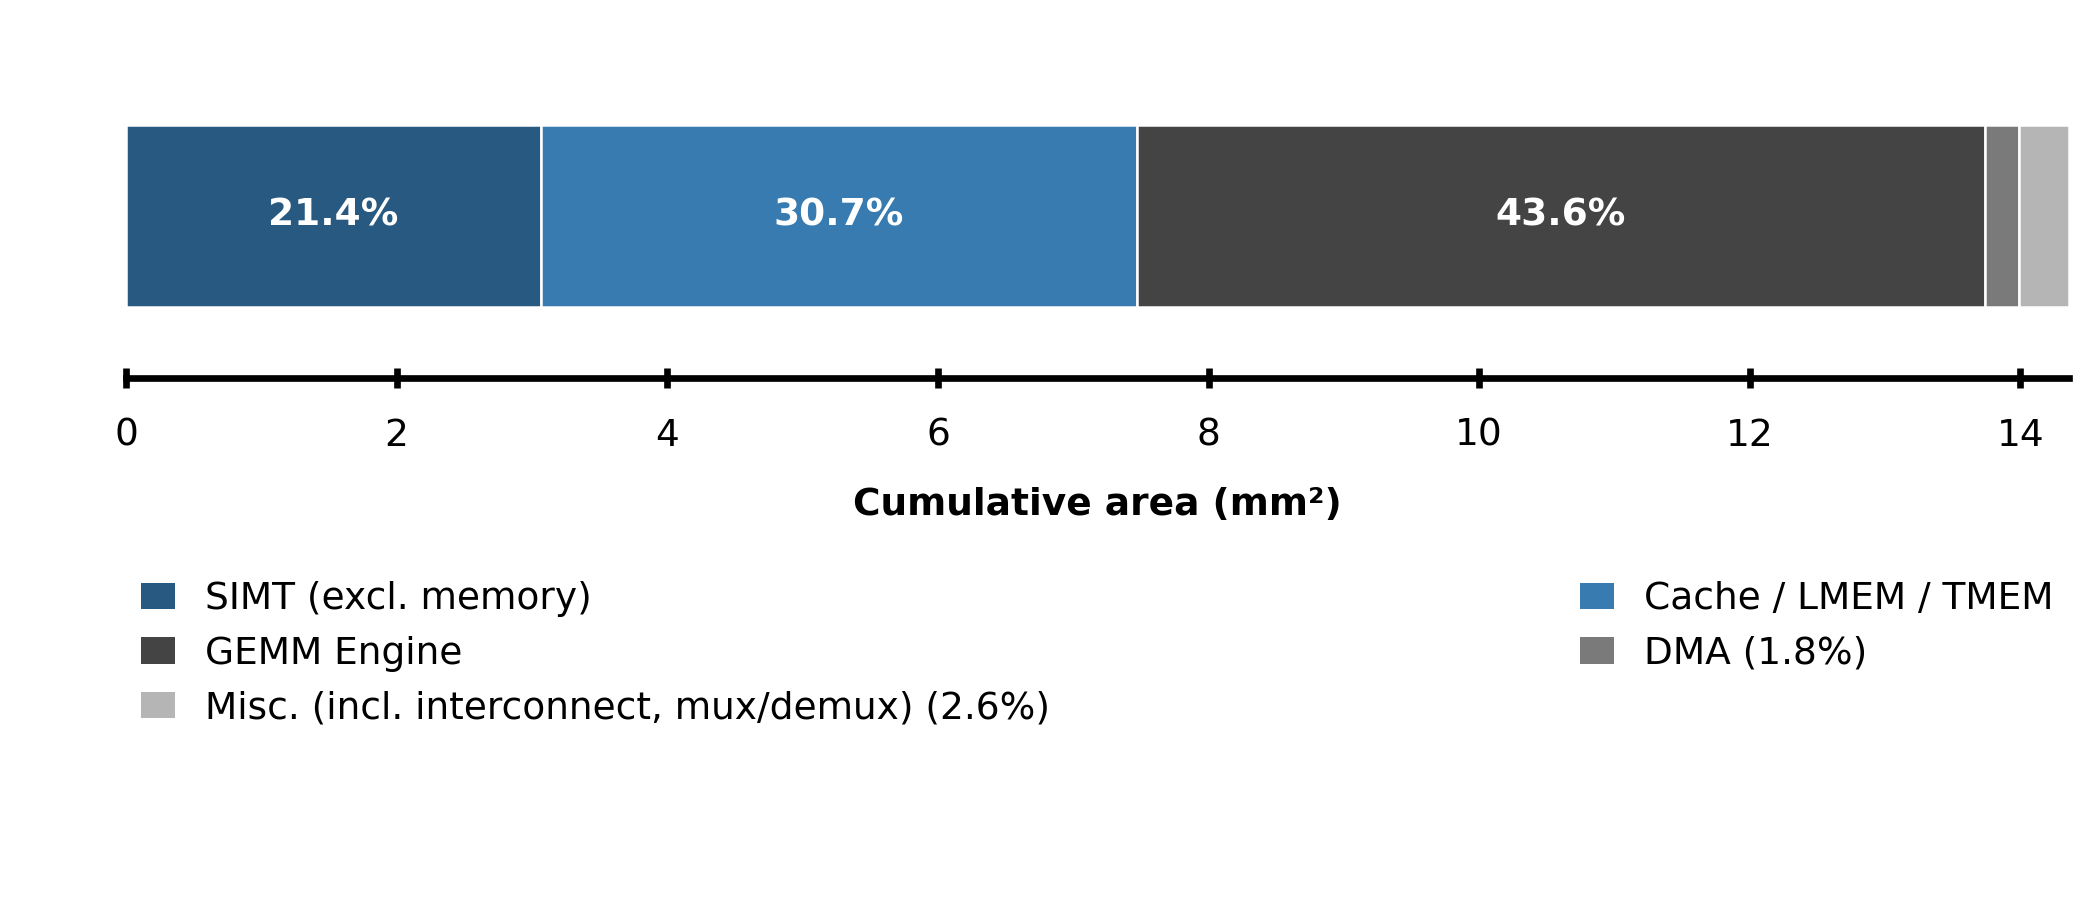
\includegraphics[width=\linewidth]{figures/top_breakdown/vortex_axi_breakdown.png}
    \caption{Full-system area breakdown of \ours{}, showing that the direct-connected tensor path keeps DMA and interconnect overhead low.}
    \label{fig:area-breakdown}
\end{figure}
\end{comment}

\FloatBarrier
\section{Conclusion}

% WKV quantization turns both linear layers and KV-attention GEMMs into \fpint{} operations, yet most prior \fpint{} accelerators accelerate only linear layers and fall back to an FP$\times$FP datapath for quantized attention. We presented \ours{}, an end-to-end system that extends native \fpint{} execution across both, combining a GEMM engine with reconfigurable quantization direction and operand-loading orientation with a dedicated tensor-memory subsystem and datapath. On an FPGA prototype evaluated through four incremental design points, \ours{} improves array-level TOPS/mm$^2$ by $2.21\times$ and TOPS/W by $2.97\times$ over the FP TCU, and across Llama2-7B and Llama3-8B W4A16KV4 inference reduces area-normalized end-to-end latency by $3.24\times$ in prefill and $4.73\times$ in decode on geomean, with energy per token lower by $3.85\times$ and $97.44\times$. Realizing the system-level benefit of WKV quantization therefore requires co-designing native \fpint{} attention support with an operand-delivery system that keeps the denser array utilized.
WKV quantization makes both linear and attention GEMMs \fpint{} operations, but prior accelerators typically retain FP attention. \ours{} supports both through reconfigurable quantization direction and operand loading, with dedicated tensor memory sustaining the denser array. It achieves $3.13\times$ the FP TCU's TOPS/mm$^2$ and $2.54\times$ its TOPS/W. On the FPGA prototype, geometric-mean end-to-end speedups over the linear-only \fpint{} baseline are $3.24\times$ in prefill and $5.93\times$ in decode, with energy per token reduced by $2.67\times$ and $8.72\times$. These results show how native quantized-attention support and operand delivery together translate array efficiency into system-level gains.


%%%%%%% -- PAPER CONTENT ENDS -- %%%%%%%%


%%%%%%%%% -- BIB STYLE AND FILE -- %%%%%%%%
\bibliographystyle{ACM-Reference-Format}
\bibliography{refs}
%%%%%%%%%%%%%%%%%%%%%%%%%%%%%%%%%%%%

% \begin{figure}[t]
%     \centering
%     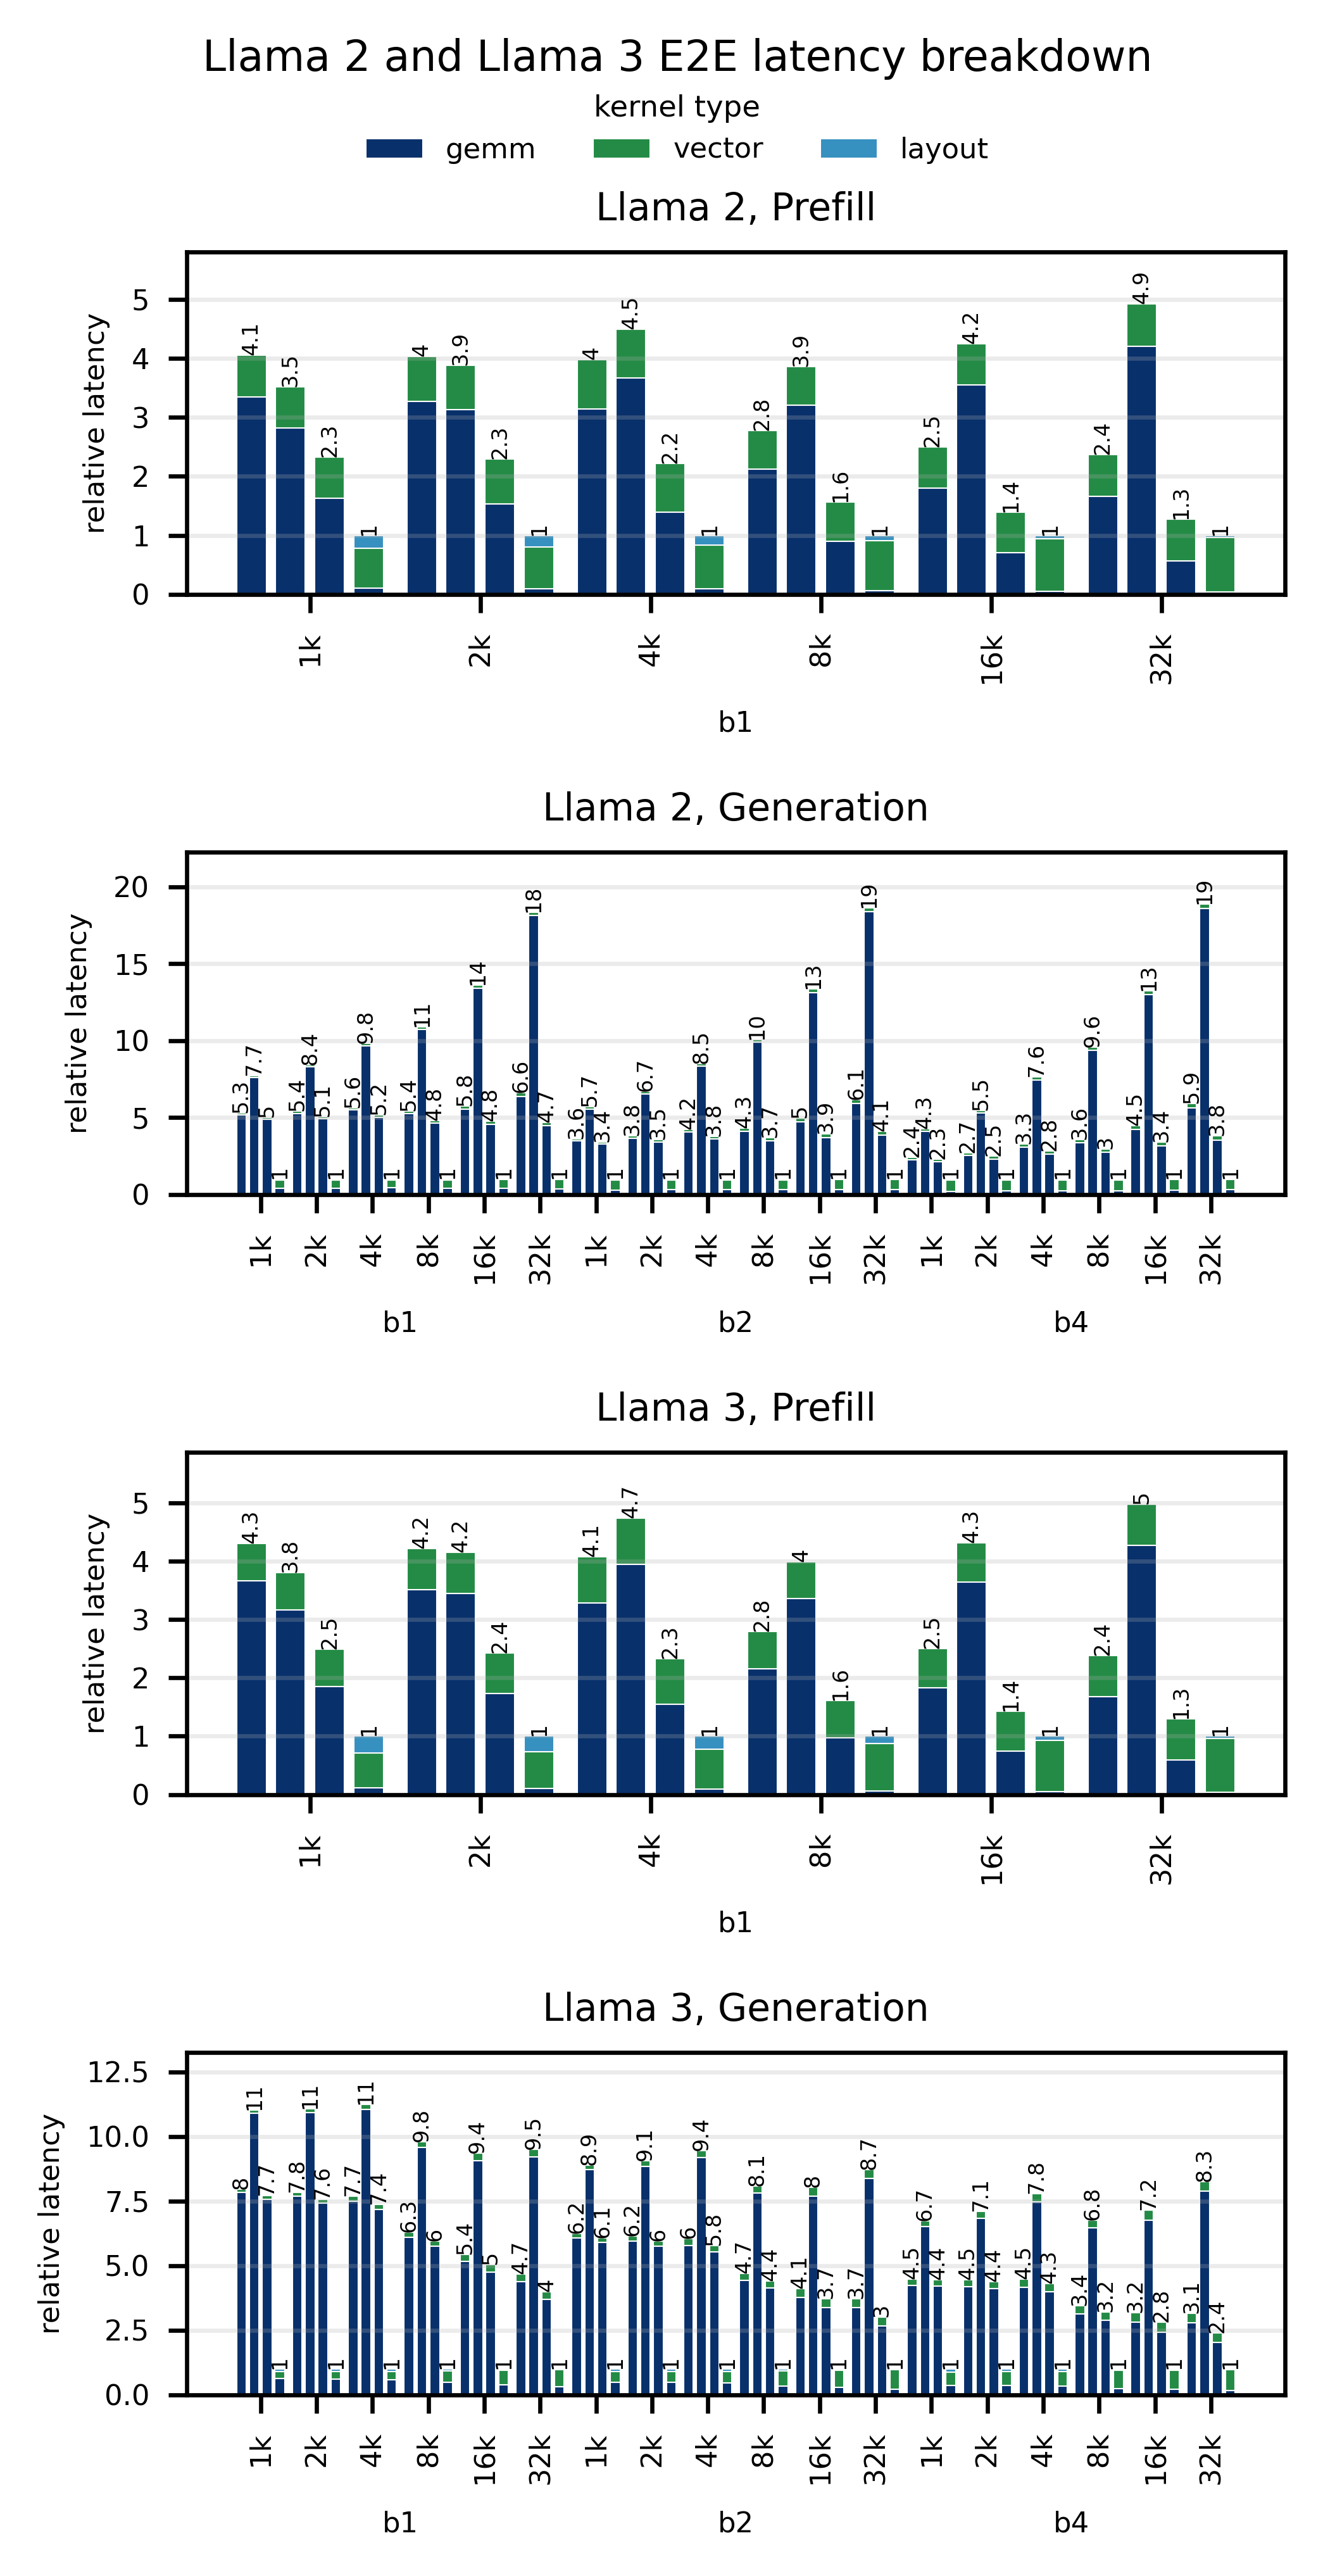
\includegraphics[width=\columnwidth]{figures/llama_e2e_latency_stacked.png}
%     \caption{one column test}
%     \label{fig:one-col-test}
% \end{figure}

\end{document}
